\documentclass[twoside]{book}

% Packages required by doxygen
\usepackage{fixltx2e}
\usepackage{calc}
\usepackage{doxygen}
\usepackage[export]{adjustbox} % also loads graphicx
\usepackage{graphicx}
\usepackage[utf8]{inputenc}
\usepackage{makeidx}
\usepackage{multicol}
\usepackage{multirow}
\PassOptionsToPackage{warn}{textcomp}
\usepackage{textcomp}
\usepackage[nointegrals]{wasysym}
\usepackage[table]{xcolor}

% Font selection
\usepackage[T1]{fontenc}
\usepackage[scaled=.90]{helvet}
\usepackage{courier}
\usepackage{amssymb}
\usepackage{sectsty}
\renewcommand{\familydefault}{\sfdefault}
\allsectionsfont{%
  \fontseries{bc}\selectfont%
  \color{darkgray}%
}
\renewcommand{\DoxyLabelFont}{%
  \fontseries{bc}\selectfont%
  \color{darkgray}%
}
\newcommand{\+}{\discretionary{\mbox{\scriptsize$\hookleftarrow$}}{}{}}

% Page & text layout
\usepackage{geometry}
\geometry{%
  a4paper,%
  top=2.5cm,%
  bottom=2.5cm,%
  left=2.5cm,%
  right=2.5cm%
}
\tolerance=750
\hfuzz=15pt
\hbadness=750
\setlength{\emergencystretch}{15pt}
\setlength{\parindent}{0cm}
\setlength{\parskip}{3ex plus 2ex minus 2ex}
\makeatletter
\renewcommand{\paragraph}{%
  \@startsection{paragraph}{4}{0ex}{-1.0ex}{1.0ex}{%
    \normalfont\normalsize\bfseries\SS@parafont%
  }%
}
\renewcommand{\subparagraph}{%
  \@startsection{subparagraph}{5}{0ex}{-1.0ex}{1.0ex}{%
    \normalfont\normalsize\bfseries\SS@subparafont%
  }%
}
\makeatother

% Headers & footers
\usepackage{fancyhdr}
\pagestyle{fancyplain}
\fancyhead[LE]{\fancyplain{}{\bfseries\thepage}}
\fancyhead[CE]{\fancyplain{}{}}
\fancyhead[RE]{\fancyplain{}{\bfseries\leftmark}}
\fancyhead[LO]{\fancyplain{}{\bfseries\rightmark}}
\fancyhead[CO]{\fancyplain{}{}}
\fancyhead[RO]{\fancyplain{}{\bfseries\thepage}}
\fancyfoot[LE]{\fancyplain{}{}}
\fancyfoot[CE]{\fancyplain{}{}}
\fancyfoot[RE]{\fancyplain{}{\bfseries\scriptsize Generated by Doxygen }}
\fancyfoot[LO]{\fancyplain{}{\bfseries\scriptsize Generated by Doxygen }}
\fancyfoot[CO]{\fancyplain{}{}}
\fancyfoot[RO]{\fancyplain{}{}}
\renewcommand{\footrulewidth}{0.4pt}
\renewcommand{\chaptermark}[1]{%
  \markboth{#1}{}%
}
\renewcommand{\sectionmark}[1]{%
  \markright{\thesection\ #1}%
}

% Indices & bibliography
\usepackage{natbib}
\usepackage[titles]{tocloft}
\setcounter{tocdepth}{3}
\setcounter{secnumdepth}{5}
\makeindex

% Hyperlinks (required, but should be loaded last)
\usepackage{ifpdf}
\ifpdf
  \usepackage[pdftex,pagebackref=true]{hyperref}
\else
  \usepackage[ps2pdf,pagebackref=true]{hyperref}
\fi
\hypersetup{%
  colorlinks=true,%
  linkcolor=blue,%
  citecolor=blue,%
  unicode%
}

% Custom commands
\newcommand{\clearemptydoublepage}{%
  \newpage{\pagestyle{empty}\cleardoublepage}%
}

\usepackage{caption}
\captionsetup{labelsep=space,justification=centering,font={bf},singlelinecheck=off,skip=4pt,position=top}

%===== C O N T E N T S =====

\begin{document}

% Titlepage & ToC
\hypersetup{pageanchor=false,
             bookmarksnumbered=true,
             pdfencoding=unicode
            }
\pagenumbering{alph}
\begin{titlepage}
\vspace*{7cm}
\begin{center}%
{\Large F\+L\+X\+S1 }\\
\vspace*{1cm}
{\large Generated by Doxygen 1.8.13}\\
\end{center}
\end{titlepage}
\clearemptydoublepage
\pagenumbering{roman}
\tableofcontents
\clearemptydoublepage
\pagenumbering{arabic}
\hypersetup{pageanchor=true}

%--- Begin generated contents ---
\chapter{Hierarchical Index}
\section{Class Hierarchy}
This inheritance list is sorted roughly, but not completely, alphabetically\+:\begin{DoxyCompactList}
\item \contentsline{section}{Display\+Module}{\pageref{class_display_module}}{}
\item \contentsline{section}{Input\+Module}{\pageref{class_input_module}}{}
\item \contentsline{section}{L\+E\+D\+Array}{\pageref{class_l_e_d_array}}{}
\item \contentsline{section}{Master\+Clock}{\pageref{class_master_clock}}{}
\item \contentsline{section}{Midi\+Module}{\pageref{class_midi_module}}{}
\item \contentsline{section}{Output\+Controller}{\pageref{class_output_controller}}{}
\item Print\begin{DoxyCompactList}
\item \contentsline{section}{Serial\+Flash\+Print}{\pageref{class_serial_flash_print}}{}
\end{DoxyCompactList}
\item \contentsline{section}{Step\+Datum}{\pageref{struct_step_datum}}{}
\item \contentsline{section}{Time\+Controller}{\pageref{class_time_controller}}{}
\end{DoxyCompactList}

\chapter{Class Index}
\section{Class List}
Here are the classes, structs, unions and interfaces with brief descriptions\+:\begin{DoxyCompactList}
\item\contentsline{section}{\hyperlink{class_display_module}{Display\+Module} }{\pageref{class_display_module}}{}
\item\contentsline{section}{\hyperlink{class_input_module}{Input\+Module} }{\pageref{class_input_module}}{}
\item\contentsline{section}{\hyperlink{class_l_e_d_array}{L\+E\+D\+Array} }{\pageref{class_l_e_d_array}}{}
\item\contentsline{section}{\hyperlink{class_master_clock}{Master\+Clock} }{\pageref{class_master_clock}}{}
\item\contentsline{section}{\hyperlink{class_midi_module}{Midi\+Module} }{\pageref{class_midi_module}}{}
\item\contentsline{section}{\hyperlink{class_output_controller}{Output\+Controller} }{\pageref{class_output_controller}}{}
\item\contentsline{section}{\hyperlink{class_serial_flash_print}{Serial\+Flash\+Print} }{\pageref{class_serial_flash_print}}{}
\item\contentsline{section}{\hyperlink{struct_step_datum}{Step\+Datum} }{\pageref{struct_step_datum}}{}
\item\contentsline{section}{\hyperlink{class_time_controller}{Time\+Controller} }{\pageref{class_time_controller}}{}
\end{DoxyCompactList}

\chapter{File Index}
\section{File List}
Here is a list of all files with brief descriptions\+:\begin{DoxyCompactList}
\item\contentsline{section}{src/\hyperlink{display_module_8cpp}{display\+Module.\+cpp} }{\pageref{display_module_8cpp}}{}
\item\contentsline{section}{src/\hyperlink{display_module_8h}{display\+Module.\+h} }{\pageref{display_module_8h}}{}
\item\contentsline{section}{src/\hyperlink{_flash_memory_8cpp}{Flash\+Memory.\+cpp} }{\pageref{_flash_memory_8cpp}}{}
\item\contentsline{section}{src/\hyperlink{_flash_memory_8h}{Flash\+Memory.\+h} }{\pageref{_flash_memory_8h}}{}
\item\contentsline{section}{src/\hyperlink{_flash_memory_cache_8cpp}{Flash\+Memory\+Cache.\+cpp} }{\pageref{_flash_memory_cache_8cpp}}{}
\item\contentsline{section}{src/\hyperlink{_flash_memory_utility_8cpp}{Flash\+Memory\+Utility.\+cpp} }{\pageref{_flash_memory_utility_8cpp}}{}
\item\contentsline{section}{src/\hyperlink{global_8cpp}{global.\+cpp} }{\pageref{global_8cpp}}{}
\item\contentsline{section}{src/\hyperlink{global_8h}{global.\+h} }{\pageref{global_8h}}{}
\item\contentsline{section}{src/\hyperlink{input_module_8cpp}{input\+Module.\+cpp} }{\pageref{input_module_8cpp}}{}
\item\contentsline{section}{src/\hyperlink{input_module_8h}{input\+Module.\+h} }{\pageref{input_module_8h}}{}
\item\contentsline{section}{src/\hyperlink{_l_e_d_array_8cpp}{L\+E\+D\+Array.\+cpp} }{\pageref{_l_e_d_array_8cpp}}{}
\item\contentsline{section}{src/\hyperlink{_l_e_d_array_8h}{L\+E\+D\+Array.\+h} }{\pageref{_l_e_d_array_8h}}{}
\item\contentsline{section}{src/\hyperlink{master_clock_8cpp}{master\+Clock.\+cpp} }{\pageref{master_clock_8cpp}}{}
\item\contentsline{section}{src/\hyperlink{master_clock_8h}{master\+Clock.\+h} }{\pageref{master_clock_8h}}{}
\item\contentsline{section}{src/\hyperlink{midi_module_8cpp}{midi\+Module.\+cpp} }{\pageref{midi_module_8cpp}}{}
\item\contentsline{section}{src/\hyperlink{midi_module_8h}{midi\+Module.\+h} }{\pageref{midi_module_8h}}{}
\item\contentsline{section}{src/\hyperlink{_output_controller_8cpp}{Output\+Controller.\+cpp} }{\pageref{_output_controller_8cpp}}{}
\item\contentsline{section}{src/\hyperlink{_output_controller_8h}{Output\+Controller.\+h} }{\pageref{_output_controller_8h}}{}
\item\contentsline{section}{src/\hyperlink{_sequencer_8cpp}{Sequencer.\+cpp} }{\pageref{_sequencer_8cpp}}{}
\item\contentsline{section}{src/\hyperlink{_sequencer_8h}{Sequencer.\+h} }{\pageref{_sequencer_8h}}{}
\item\contentsline{section}{src/\hyperlink{serial_flash_print_8cpp}{serial\+Flash\+Print.\+cpp} }{\pageref{serial_flash_print_8cpp}}{}
\item\contentsline{section}{src/\hyperlink{serial_flash_print_8h}{serial\+Flash\+Print.\+h} }{\pageref{serial_flash_print_8h}}{}
\item\contentsline{section}{src/\hyperlink{_step_datum_8h}{Step\+Datum.\+h} }{\pageref{_step_datum_8h}}{}
\item\contentsline{section}{src/\hyperlink{_time_controller_8cpp}{Time\+Controller.\+cpp} }{\pageref{_time_controller_8cpp}}{}
\item\contentsline{section}{src/\hyperlink{_time_controller_8h}{Time\+Controller.\+h} }{\pageref{_time_controller_8h}}{}
\end{DoxyCompactList}

\chapter{Class Documentation}
\hypertarget{class_display_module}{}\section{Display\+Module Class Reference}
\label{class_display_module}\index{Display\+Module@{Display\+Module}}


{\ttfamily \#include $<$display\+Module.\+h$>$}

\subsection*{Public Member Functions}
\begin{DoxyCompactItemize}
\item 
\hyperlink{class_display_module_a6e39f0daba38d7d919ebece3e85c24b1}{Display\+Module} ()
\item 
void \hyperlink{class_display_module_a68451c130f98f5d820377e9aa15a7242}{initialize} (Sequencer $\ast$\hyperlink{class_display_module_a9eb0f63acb02bc366bdc36cf60efb799}{sequence\+Array})
\item 
void \hyperlink{class_display_module_ab89f4bb8387cd4a0557b23ee14133568}{display\+Loop} (uint16\+\_\+t \hyperlink{global_8h_acdfc8898c9e67fbcec81f3b04ae61bd9}{frequency})
\item 
void \hyperlink{class_display_module_a1e2ecbe240db8c38bea2839a76c566f0}{clear\+Display} ()
\item 
void \hyperlink{class_display_module_a4eb1fdb54d5ce4e0b8e460d30b443aac}{free\+Display\+Cache} ()
\item 
void \hyperlink{class_display_module_ac1d55595826fc36738b2d9df6be9516e}{step\+Display} (char $\ast$\hyperlink{class_display_module_a07c140067fde1f0cbc4061296179d69a}{buf})
\item 
void \hyperlink{class_display_module_a95fa96a6b2d74b8d15eeb0c71786b1b2}{pattern\+Select\+Display} ()
\item 
void \hyperlink{class_display_module_a61c9ecea836833a5460f2834a18eef05}{channel\+Pitch\+Menu\+Display} (char $\ast$\hyperlink{class_display_module_a07c140067fde1f0cbc4061296179d69a}{buf})
\item 
void \hyperlink{class_display_module_a5e665571a41c10190dd2015489f87f3e}{channel\+Pitch\+Menu\+Display2} (char $\ast$\hyperlink{class_display_module_a07c140067fde1f0cbc4061296179d69a}{buf})
\item 
void \hyperlink{class_display_module_afb4cbf31bb1058fdeceb3d10ae7fe3a6}{channel\+Velocity\+Menu\+Display} (char $\ast$\hyperlink{class_display_module_a07c140067fde1f0cbc4061296179d69a}{buf})
\item 
void \hyperlink{class_display_module_a61256f4c2a099fd0b0c59a5bba277914}{channel\+Envelope\+Menu\+Display} (char $\ast$\hyperlink{class_display_module_a07c140067fde1f0cbc4061296179d69a}{buf})
\item 
void \hyperlink{class_display_module_ad5607972b28b5da028dda61cfe640638}{channel\+Step\+Menu\+Display} (char $\ast$\hyperlink{class_display_module_a07c140067fde1f0cbc4061296179d69a}{buf})
\item 
void \hyperlink{class_display_module_a579629d520ad24f721a25b9b1340516b}{channel\+Tuner\+Display} (char $\ast$\hyperlink{class_display_module_a07c140067fde1f0cbc4061296179d69a}{buf})
\item 
void \hyperlink{class_display_module_a3e2fc0a60ef41f41e57d463faf59bd2b}{sequence\+Menu\+Display} ()
\item 
void \hyperlink{class_display_module_a5082cabe11332dc4a9d0daea8a60f9dc}{global\+Menu\+Display} ()
\item 
void \hyperlink{class_display_module_ac5999c2f0f4b1ecc12bafe7094c7b7d2}{tempo\+Menu\+Display} ()
\item 
void \hyperlink{class_display_module_a38006afa64e93afb6c259b137f45bcde}{game\+Of\+Life\+Display} ()
\item 
void \hyperlink{class_display_module_a87e0b873a0f1fcec1bc67f2fa7c9739a}{delete\+Menu\+Display} ()
\item 
void \hyperlink{class_display_module_ab730677e34ecadf39916f9b71c2a41fe}{cleanup\+Text\+Buffers} ()
\item 
void \hyperlink{class_display_module_a722a8c3b1cce1c58fa7e17e2865c3e57}{timing\+Menu\+Display} ()
\item 
void \hyperlink{class_display_module_ae68c2f34985c276b559df3d7f4fafbbd}{calibration\+Menu\+Display} ()
\item 
void \hyperlink{class_display_module_a776e918a0d9f50ae079d6839524cc471}{input\+Debug\+Menu\+Display} ()
\item 
void \hyperlink{class_display_module_a453ceefb9e2a9a82dd7b62825cc2cac8}{render\+Once\+\_\+\+String\+Box} (uint8\+\_\+t index, uint8\+\_\+t \hyperlink{class_display_module_a33ee7436481d6285fb6c81166711fbce}{highlight}, uint8\+\_\+t previous\+Highlight, int16\+\_\+t x, int16\+\_\+t y, int16\+\_\+t w, int16\+\_\+t h, bool border, uint8\+\_\+t text\+Size, uint16\+\_\+t \hyperlink{class_display_module_ac071b7f3b2027d0e90b7d3031d61a99b}{color}, uint16\+\_\+t bg\+Color)
\end{DoxyCompactItemize}
\subsection*{Public Attributes}
\begin{DoxyCompactItemize}
\item 
int \hyperlink{class_display_module_ac071b7f3b2027d0e90b7d3031d61a99b}{color} = 0
\item 
uint32\+\_\+t \hyperlink{class_display_module_a5c8825161e8df40668c79145e5dace28}{runcount}
\item 
char $\ast$ \hyperlink{class_display_module_adf0d12d4d19fa7bff2fc66411e4255a2}{display\+Cache} \mbox{[}\hyperlink{display_module_8h_a6114392da1243b69a45b549bd4ddfd39}{M\+A\+X\+\_\+\+D\+I\+S\+P\+L\+A\+Y\+\_\+\+E\+L\+E\+M\+E\+N\+TS}\mbox{]}
\item 
char $\ast$ \hyperlink{class_display_module_a7af82afb24a27ab297fda02a9d1f0eb3}{display\+Element} \mbox{[}\hyperlink{display_module_8h_a6114392da1243b69a45b549bd4ddfd39}{M\+A\+X\+\_\+\+D\+I\+S\+P\+L\+A\+Y\+\_\+\+E\+L\+E\+M\+E\+N\+TS}\mbox{]}
\item 
char $\ast$ \hyperlink{class_display_module_a07c140067fde1f0cbc4061296179d69a}{buf} = new char\mbox{[}51\mbox{]}
\item 
uint8\+\_\+t \hyperlink{class_display_module_a33ee7436481d6285fb6c81166711fbce}{highlight}
\item 
uint8\+\_\+t \hyperlink{class_display_module_aaca9b1f6821215e5ebdc5bb6edb390b8}{previously\+Selected\+Channel}
\item 
S\+S\+D\+\_\+13\+XX \hyperlink{class_display_module_abcfa732c08671b60dbf7f8d7e0d17e74}{oled} = S\+S\+D\+\_\+13\+XX(\hyperlink{display_module_8h_a71d24cab0e16b054de228f29139f1b79}{L\+C\+D\+\_\+\+CS}, \hyperlink{display_module_8h_a1dc6c4886242abf4447d0da651125d5d}{L\+C\+D\+\_\+\+DC}, \hyperlink{display_module_8h_aec0f0ab242f1b58b1d017bc9ab4b898b}{L\+C\+D\+\_\+\+R\+ST})
\item 
elapsed\+Micros \hyperlink{class_display_module_a0c92fa8b35e030ef848db6207fe5067b}{display\+Timer}
\item 
uint16\+\_\+t \hyperlink{class_display_module_ab3b6b57d36f08a63a68641eefdb56446}{foreground}
\item 
uint16\+\_\+t \hyperlink{class_display_module_a7ebe1c30eb4c306a99a3129f6a165e2a}{background}
\end{DoxyCompactItemize}
\subsection*{Private Attributes}
\begin{DoxyCompactItemize}
\item 
Sequencer $\ast$ \hyperlink{class_display_module_a9eb0f63acb02bc366bdc36cf60efb799}{sequence\+Array}
\item 
const char $\ast$ \hyperlink{class_display_module_a76bde3057832542df04f4796ae917d48}{midi\+Notes} \mbox{[}128\mbox{]}
\end{DoxyCompactItemize}


\subsection{Constructor \& Destructor Documentation}
\mbox{\Hypertarget{class_display_module_a6e39f0daba38d7d919ebece3e85c24b1}\label{class_display_module_a6e39f0daba38d7d919ebece3e85c24b1}} 
\index{Display\+Module@{Display\+Module}!Display\+Module@{Display\+Module}}
\index{Display\+Module@{Display\+Module}!Display\+Module@{Display\+Module}}
\subsubsection{\texorpdfstring{Display\+Module()}{DisplayModule()}}
{\footnotesize\ttfamily Display\+Module\+::\+Display\+Module (\begin{DoxyParamCaption}{ }\end{DoxyParamCaption})}



\subsection{Member Function Documentation}
\mbox{\Hypertarget{class_display_module_ae68c2f34985c276b559df3d7f4fafbbd}\label{class_display_module_ae68c2f34985c276b559df3d7f4fafbbd}} 
\index{Display\+Module@{Display\+Module}!calibration\+Menu\+Display@{calibration\+Menu\+Display}}
\index{calibration\+Menu\+Display@{calibration\+Menu\+Display}!Display\+Module@{Display\+Module}}
\subsubsection{\texorpdfstring{calibration\+Menu\+Display()}{calibrationMenuDisplay()}}
{\footnotesize\ttfamily void Display\+Module\+::calibration\+Menu\+Display (\begin{DoxyParamCaption}{ }\end{DoxyParamCaption})}

Here is the call graph for this function\+:
\nopagebreak
\begin{figure}[H]
\begin{center}
\leavevmode
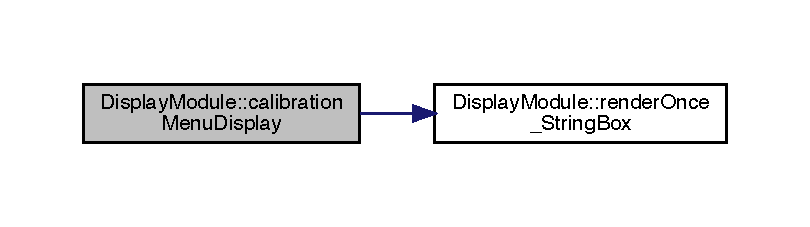
\includegraphics[width=350pt]{class_display_module_ae68c2f34985c276b559df3d7f4fafbbd_cgraph}
\end{center}
\end{figure}
Here is the caller graph for this function\+:
\nopagebreak
\begin{figure}[H]
\begin{center}
\leavevmode
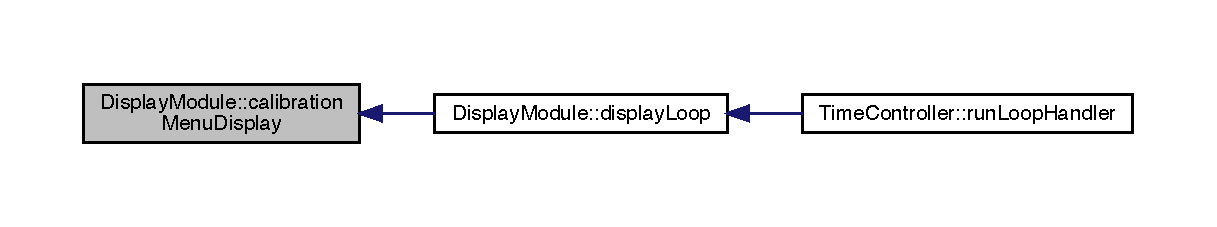
\includegraphics[width=350pt]{class_display_module_ae68c2f34985c276b559df3d7f4fafbbd_icgraph}
\end{center}
\end{figure}
\mbox{\Hypertarget{class_display_module_a61256f4c2a099fd0b0c59a5bba277914}\label{class_display_module_a61256f4c2a099fd0b0c59a5bba277914}} 
\index{Display\+Module@{Display\+Module}!channel\+Envelope\+Menu\+Display@{channel\+Envelope\+Menu\+Display}}
\index{channel\+Envelope\+Menu\+Display@{channel\+Envelope\+Menu\+Display}!Display\+Module@{Display\+Module}}
\subsubsection{\texorpdfstring{channel\+Envelope\+Menu\+Display()}{channelEnvelopeMenuDisplay()}}
{\footnotesize\ttfamily void Display\+Module\+::channel\+Envelope\+Menu\+Display (\begin{DoxyParamCaption}\item[{char $\ast$}]{buf }\end{DoxyParamCaption})}

Here is the call graph for this function\+:
\nopagebreak
\begin{figure}[H]
\begin{center}
\leavevmode
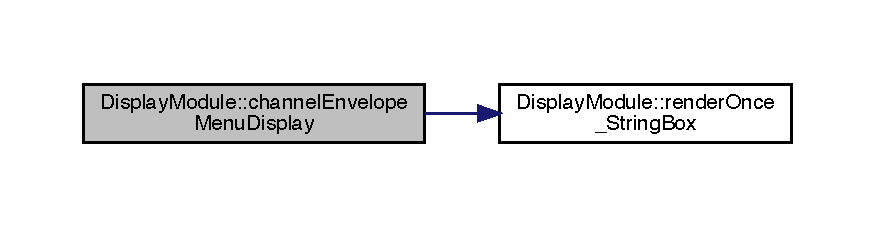
\includegraphics[width=350pt]{class_display_module_a61256f4c2a099fd0b0c59a5bba277914_cgraph}
\end{center}
\end{figure}
Here is the caller graph for this function\+:
\nopagebreak
\begin{figure}[H]
\begin{center}
\leavevmode
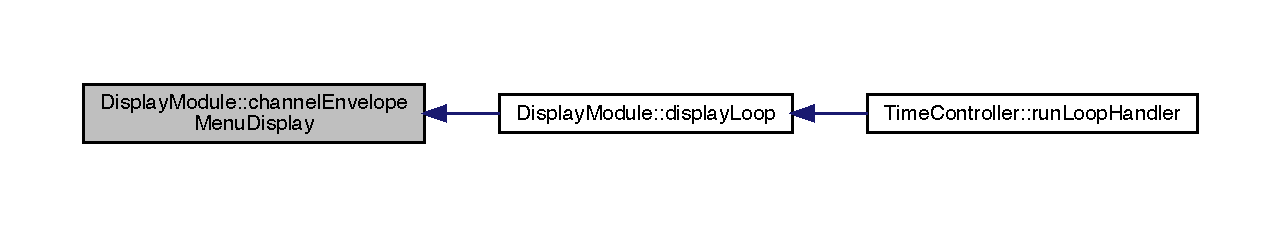
\includegraphics[width=350pt]{class_display_module_a61256f4c2a099fd0b0c59a5bba277914_icgraph}
\end{center}
\end{figure}
\mbox{\Hypertarget{class_display_module_a61c9ecea836833a5460f2834a18eef05}\label{class_display_module_a61c9ecea836833a5460f2834a18eef05}} 
\index{Display\+Module@{Display\+Module}!channel\+Pitch\+Menu\+Display@{channel\+Pitch\+Menu\+Display}}
\index{channel\+Pitch\+Menu\+Display@{channel\+Pitch\+Menu\+Display}!Display\+Module@{Display\+Module}}
\subsubsection{\texorpdfstring{channel\+Pitch\+Menu\+Display()}{channelPitchMenuDisplay()}}
{\footnotesize\ttfamily void Display\+Module\+::channel\+Pitch\+Menu\+Display (\begin{DoxyParamCaption}\item[{char $\ast$}]{buf }\end{DoxyParamCaption})}

Here is the call graph for this function\+:
\nopagebreak
\begin{figure}[H]
\begin{center}
\leavevmode
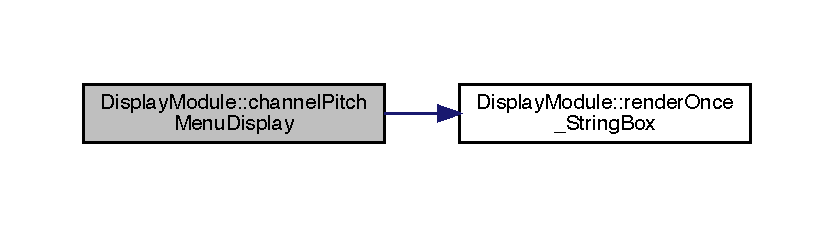
\includegraphics[width=350pt]{class_display_module_a61c9ecea836833a5460f2834a18eef05_cgraph}
\end{center}
\end{figure}
Here is the caller graph for this function\+:
\nopagebreak
\begin{figure}[H]
\begin{center}
\leavevmode
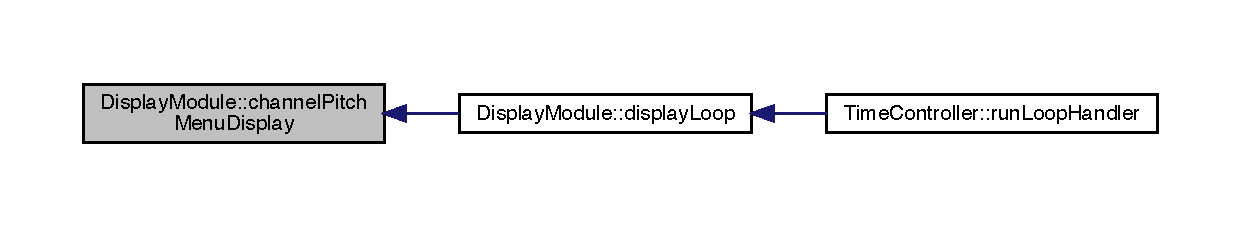
\includegraphics[width=350pt]{class_display_module_a61c9ecea836833a5460f2834a18eef05_icgraph}
\end{center}
\end{figure}
\mbox{\Hypertarget{class_display_module_a5e665571a41c10190dd2015489f87f3e}\label{class_display_module_a5e665571a41c10190dd2015489f87f3e}} 
\index{Display\+Module@{Display\+Module}!channel\+Pitch\+Menu\+Display2@{channel\+Pitch\+Menu\+Display2}}
\index{channel\+Pitch\+Menu\+Display2@{channel\+Pitch\+Menu\+Display2}!Display\+Module@{Display\+Module}}
\subsubsection{\texorpdfstring{channel\+Pitch\+Menu\+Display2()}{channelPitchMenuDisplay2()}}
{\footnotesize\ttfamily void Display\+Module\+::channel\+Pitch\+Menu\+Display2 (\begin{DoxyParamCaption}\item[{char $\ast$}]{buf }\end{DoxyParamCaption})}

Here is the call graph for this function\+:
\nopagebreak
\begin{figure}[H]
\begin{center}
\leavevmode
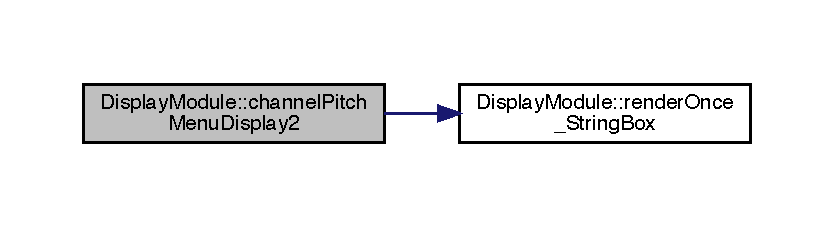
\includegraphics[width=350pt]{class_display_module_a5e665571a41c10190dd2015489f87f3e_cgraph}
\end{center}
\end{figure}
\mbox{\Hypertarget{class_display_module_ad5607972b28b5da028dda61cfe640638}\label{class_display_module_ad5607972b28b5da028dda61cfe640638}} 
\index{Display\+Module@{Display\+Module}!channel\+Step\+Menu\+Display@{channel\+Step\+Menu\+Display}}
\index{channel\+Step\+Menu\+Display@{channel\+Step\+Menu\+Display}!Display\+Module@{Display\+Module}}
\subsubsection{\texorpdfstring{channel\+Step\+Menu\+Display()}{channelStepMenuDisplay()}}
{\footnotesize\ttfamily void Display\+Module\+::channel\+Step\+Menu\+Display (\begin{DoxyParamCaption}\item[{char $\ast$}]{buf }\end{DoxyParamCaption})}

Here is the call graph for this function\+:
\nopagebreak
\begin{figure}[H]
\begin{center}
\leavevmode
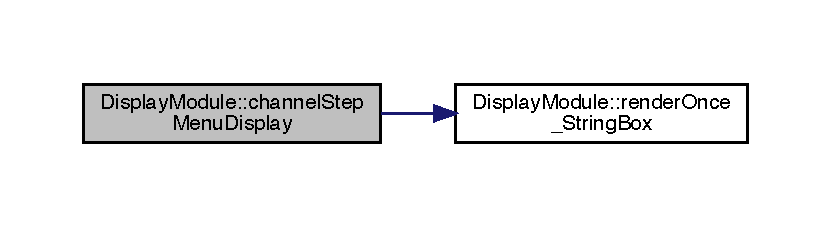
\includegraphics[width=350pt]{class_display_module_ad5607972b28b5da028dda61cfe640638_cgraph}
\end{center}
\end{figure}
Here is the caller graph for this function\+:
\nopagebreak
\begin{figure}[H]
\begin{center}
\leavevmode
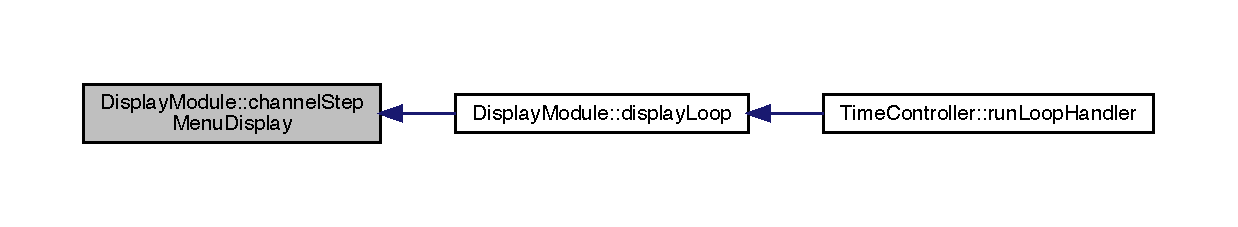
\includegraphics[width=350pt]{class_display_module_ad5607972b28b5da028dda61cfe640638_icgraph}
\end{center}
\end{figure}
\mbox{\Hypertarget{class_display_module_a579629d520ad24f721a25b9b1340516b}\label{class_display_module_a579629d520ad24f721a25b9b1340516b}} 
\index{Display\+Module@{Display\+Module}!channel\+Tuner\+Display@{channel\+Tuner\+Display}}
\index{channel\+Tuner\+Display@{channel\+Tuner\+Display}!Display\+Module@{Display\+Module}}
\subsubsection{\texorpdfstring{channel\+Tuner\+Display()}{channelTunerDisplay()}}
{\footnotesize\ttfamily void Display\+Module\+::channel\+Tuner\+Display (\begin{DoxyParamCaption}\item[{char $\ast$}]{buf }\end{DoxyParamCaption})}

Here is the call graph for this function\+:
\nopagebreak
\begin{figure}[H]
\begin{center}
\leavevmode
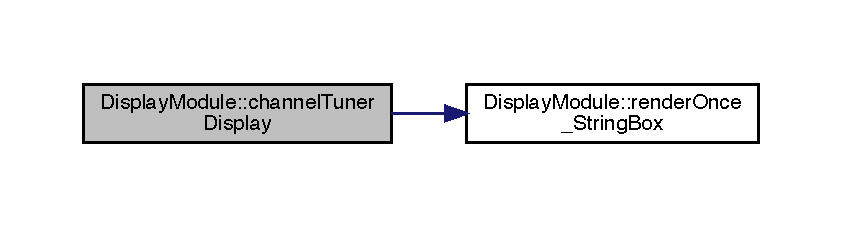
\includegraphics[width=350pt]{class_display_module_a579629d520ad24f721a25b9b1340516b_cgraph}
\end{center}
\end{figure}
Here is the caller graph for this function\+:
\nopagebreak
\begin{figure}[H]
\begin{center}
\leavevmode
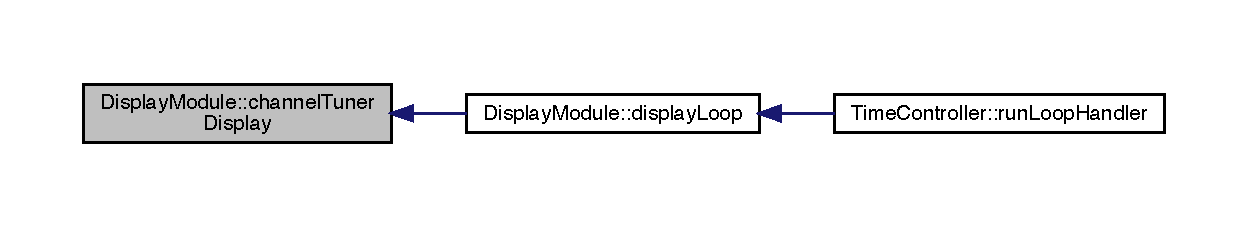
\includegraphics[width=350pt]{class_display_module_a579629d520ad24f721a25b9b1340516b_icgraph}
\end{center}
\end{figure}
\mbox{\Hypertarget{class_display_module_afb4cbf31bb1058fdeceb3d10ae7fe3a6}\label{class_display_module_afb4cbf31bb1058fdeceb3d10ae7fe3a6}} 
\index{Display\+Module@{Display\+Module}!channel\+Velocity\+Menu\+Display@{channel\+Velocity\+Menu\+Display}}
\index{channel\+Velocity\+Menu\+Display@{channel\+Velocity\+Menu\+Display}!Display\+Module@{Display\+Module}}
\subsubsection{\texorpdfstring{channel\+Velocity\+Menu\+Display()}{channelVelocityMenuDisplay()}}
{\footnotesize\ttfamily void Display\+Module\+::channel\+Velocity\+Menu\+Display (\begin{DoxyParamCaption}\item[{char $\ast$}]{buf }\end{DoxyParamCaption})}

Here is the call graph for this function\+:
\nopagebreak
\begin{figure}[H]
\begin{center}
\leavevmode
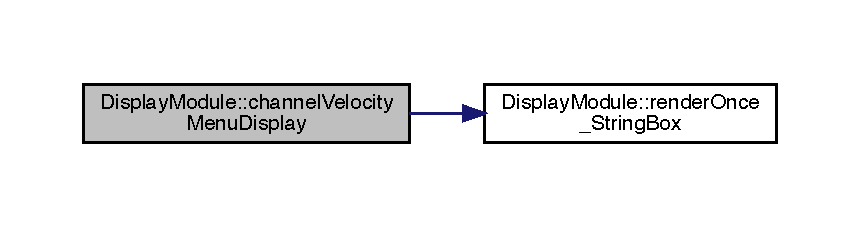
\includegraphics[width=350pt]{class_display_module_afb4cbf31bb1058fdeceb3d10ae7fe3a6_cgraph}
\end{center}
\end{figure}
Here is the caller graph for this function\+:
\nopagebreak
\begin{figure}[H]
\begin{center}
\leavevmode
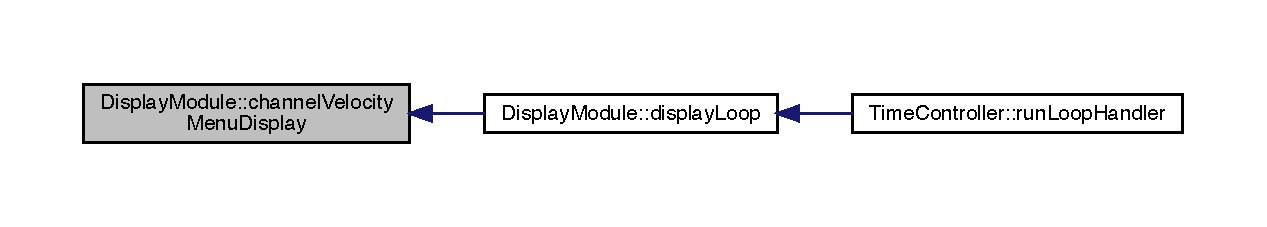
\includegraphics[width=350pt]{class_display_module_afb4cbf31bb1058fdeceb3d10ae7fe3a6_icgraph}
\end{center}
\end{figure}
\mbox{\Hypertarget{class_display_module_ab730677e34ecadf39916f9b71c2a41fe}\label{class_display_module_ab730677e34ecadf39916f9b71c2a41fe}} 
\index{Display\+Module@{Display\+Module}!cleanup\+Text\+Buffers@{cleanup\+Text\+Buffers}}
\index{cleanup\+Text\+Buffers@{cleanup\+Text\+Buffers}!Display\+Module@{Display\+Module}}
\subsubsection{\texorpdfstring{cleanup\+Text\+Buffers()}{cleanupTextBuffers()}}
{\footnotesize\ttfamily void Display\+Module\+::cleanup\+Text\+Buffers (\begin{DoxyParamCaption}{ }\end{DoxyParamCaption})}

Here is the caller graph for this function\+:
\nopagebreak
\begin{figure}[H]
\begin{center}
\leavevmode
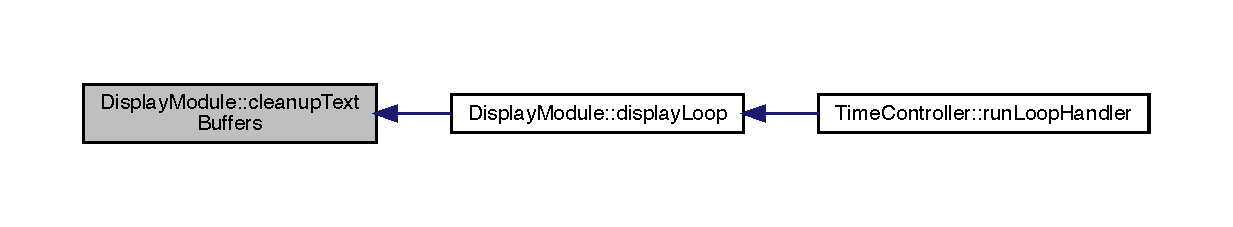
\includegraphics[width=350pt]{class_display_module_ab730677e34ecadf39916f9b71c2a41fe_icgraph}
\end{center}
\end{figure}
\mbox{\Hypertarget{class_display_module_a1e2ecbe240db8c38bea2839a76c566f0}\label{class_display_module_a1e2ecbe240db8c38bea2839a76c566f0}} 
\index{Display\+Module@{Display\+Module}!clear\+Display@{clear\+Display}}
\index{clear\+Display@{clear\+Display}!Display\+Module@{Display\+Module}}
\subsubsection{\texorpdfstring{clear\+Display()}{clearDisplay()}}
{\footnotesize\ttfamily void Display\+Module\+::clear\+Display (\begin{DoxyParamCaption}{ }\end{DoxyParamCaption})}

\mbox{\Hypertarget{class_display_module_a87e0b873a0f1fcec1bc67f2fa7c9739a}\label{class_display_module_a87e0b873a0f1fcec1bc67f2fa7c9739a}} 
\index{Display\+Module@{Display\+Module}!delete\+Menu\+Display@{delete\+Menu\+Display}}
\index{delete\+Menu\+Display@{delete\+Menu\+Display}!Display\+Module@{Display\+Module}}
\subsubsection{\texorpdfstring{delete\+Menu\+Display()}{deleteMenuDisplay()}}
{\footnotesize\ttfamily void Display\+Module\+::delete\+Menu\+Display (\begin{DoxyParamCaption}{ }\end{DoxyParamCaption})}

Here is the caller graph for this function\+:
\nopagebreak
\begin{figure}[H]
\begin{center}
\leavevmode
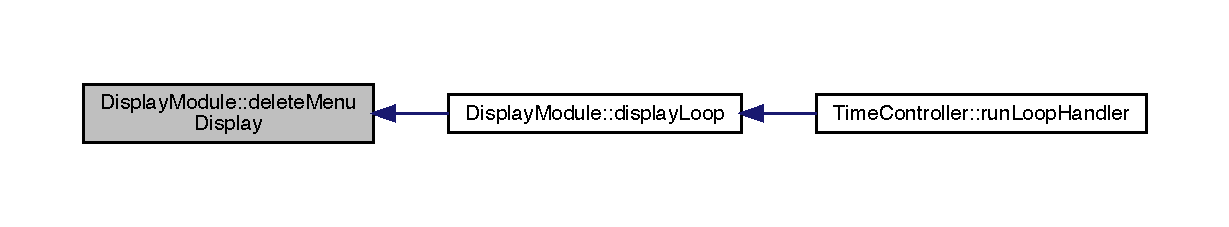
\includegraphics[width=350pt]{class_display_module_a87e0b873a0f1fcec1bc67f2fa7c9739a_icgraph}
\end{center}
\end{figure}
\mbox{\Hypertarget{class_display_module_ab89f4bb8387cd4a0557b23ee14133568}\label{class_display_module_ab89f4bb8387cd4a0557b23ee14133568}} 
\index{Display\+Module@{Display\+Module}!display\+Loop@{display\+Loop}}
\index{display\+Loop@{display\+Loop}!Display\+Module@{Display\+Module}}
\subsubsection{\texorpdfstring{display\+Loop()}{displayLoop()}}
{\footnotesize\ttfamily void Display\+Module\+::display\+Loop (\begin{DoxyParamCaption}\item[{uint16\+\_\+t}]{frequency }\end{DoxyParamCaption})}

Here is the call graph for this function\+:
\nopagebreak
\begin{figure}[H]
\begin{center}
\leavevmode
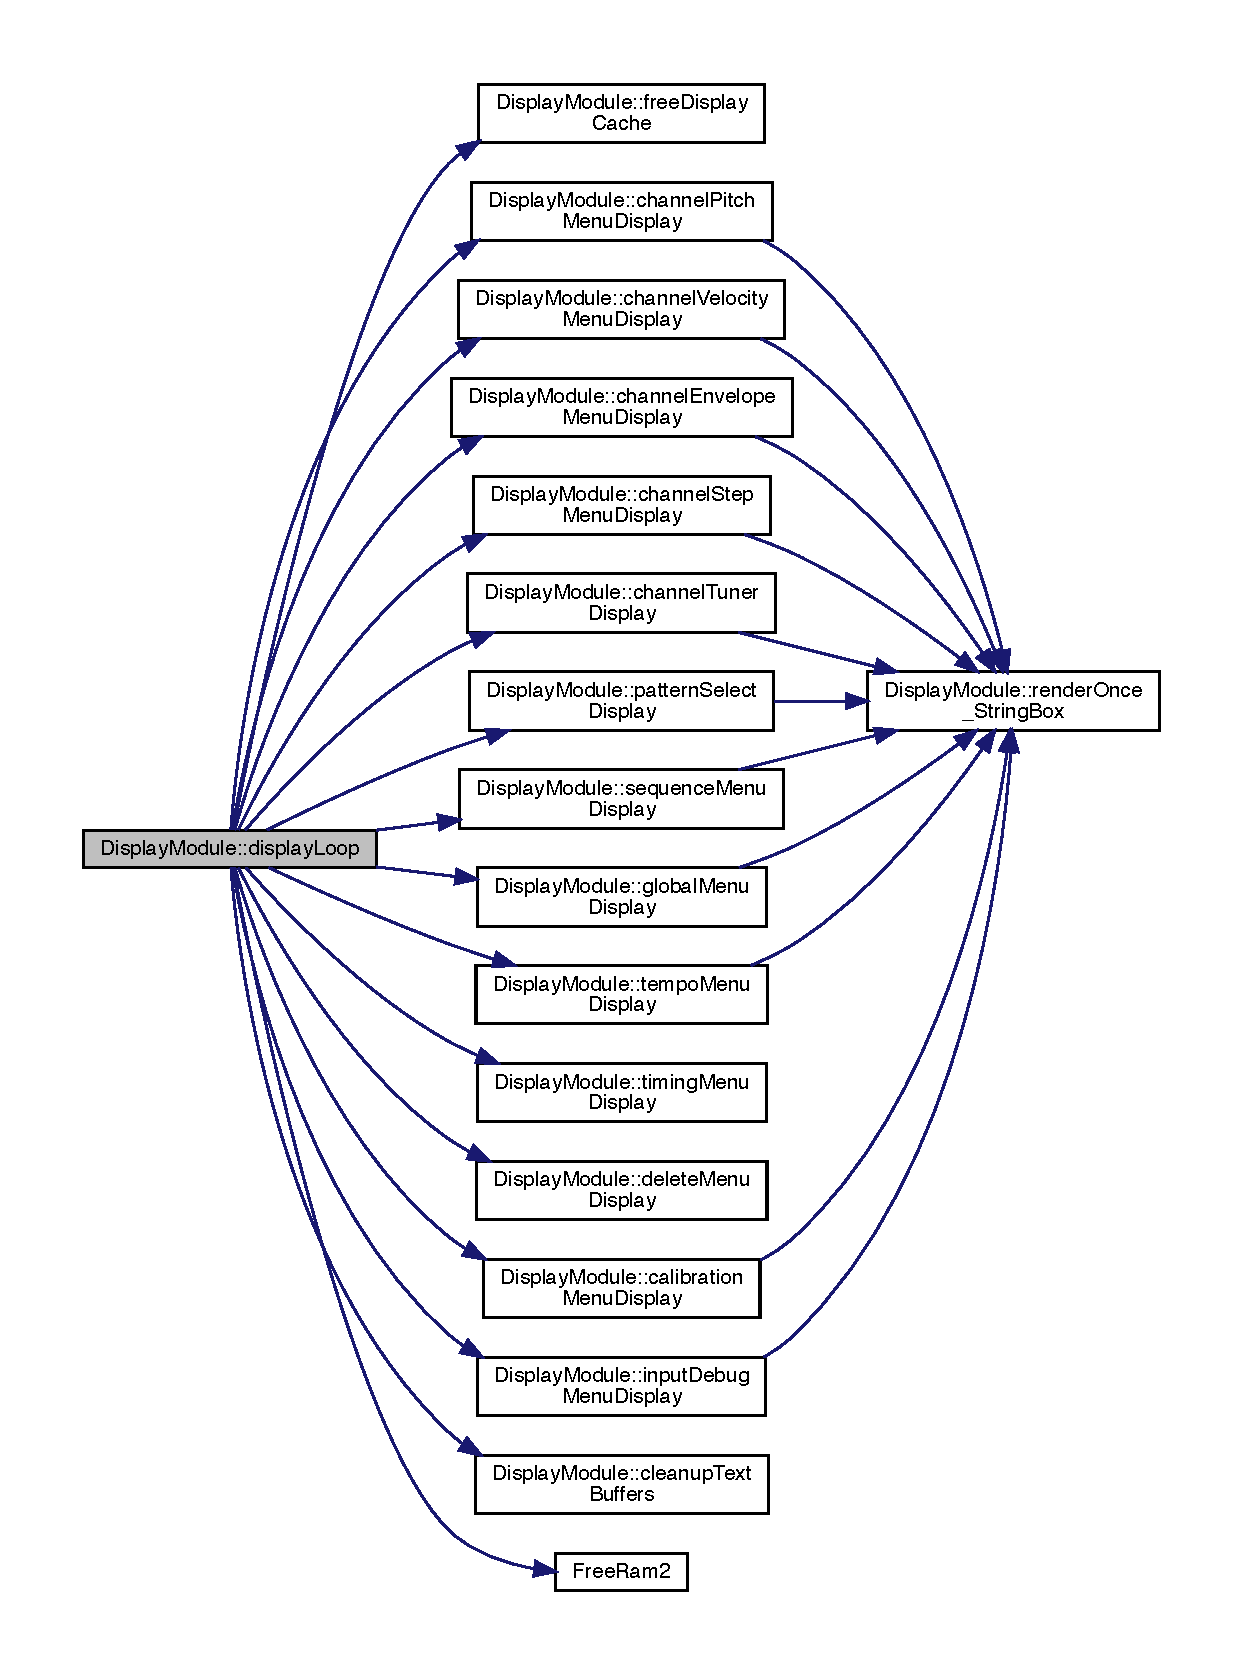
\includegraphics[width=350pt]{class_display_module_ab89f4bb8387cd4a0557b23ee14133568_cgraph}
\end{center}
\end{figure}
Here is the caller graph for this function\+:
\nopagebreak
\begin{figure}[H]
\begin{center}
\leavevmode
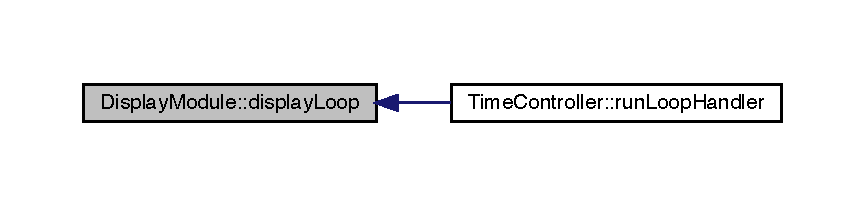
\includegraphics[width=350pt]{class_display_module_ab89f4bb8387cd4a0557b23ee14133568_icgraph}
\end{center}
\end{figure}
\mbox{\Hypertarget{class_display_module_a4eb1fdb54d5ce4e0b8e460d30b443aac}\label{class_display_module_a4eb1fdb54d5ce4e0b8e460d30b443aac}} 
\index{Display\+Module@{Display\+Module}!free\+Display\+Cache@{free\+Display\+Cache}}
\index{free\+Display\+Cache@{free\+Display\+Cache}!Display\+Module@{Display\+Module}}
\subsubsection{\texorpdfstring{free\+Display\+Cache()}{freeDisplayCache()}}
{\footnotesize\ttfamily void Display\+Module\+::free\+Display\+Cache (\begin{DoxyParamCaption}{ }\end{DoxyParamCaption})}

Here is the caller graph for this function\+:
\nopagebreak
\begin{figure}[H]
\begin{center}
\leavevmode
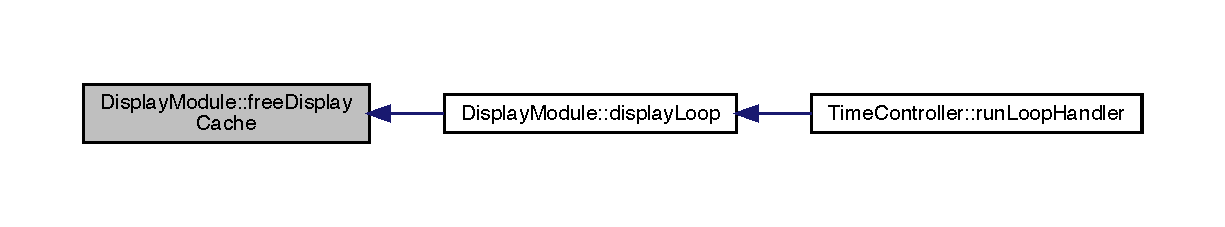
\includegraphics[width=350pt]{class_display_module_a4eb1fdb54d5ce4e0b8e460d30b443aac_icgraph}
\end{center}
\end{figure}
\mbox{\Hypertarget{class_display_module_a38006afa64e93afb6c259b137f45bcde}\label{class_display_module_a38006afa64e93afb6c259b137f45bcde}} 
\index{Display\+Module@{Display\+Module}!game\+Of\+Life\+Display@{game\+Of\+Life\+Display}}
\index{game\+Of\+Life\+Display@{game\+Of\+Life\+Display}!Display\+Module@{Display\+Module}}
\subsubsection{\texorpdfstring{game\+Of\+Life\+Display()}{gameOfLifeDisplay()}}
{\footnotesize\ttfamily void Display\+Module\+::game\+Of\+Life\+Display (\begin{DoxyParamCaption}{ }\end{DoxyParamCaption})}

\mbox{\Hypertarget{class_display_module_a5082cabe11332dc4a9d0daea8a60f9dc}\label{class_display_module_a5082cabe11332dc4a9d0daea8a60f9dc}} 
\index{Display\+Module@{Display\+Module}!global\+Menu\+Display@{global\+Menu\+Display}}
\index{global\+Menu\+Display@{global\+Menu\+Display}!Display\+Module@{Display\+Module}}
\subsubsection{\texorpdfstring{global\+Menu\+Display()}{globalMenuDisplay()}}
{\footnotesize\ttfamily void Display\+Module\+::global\+Menu\+Display (\begin{DoxyParamCaption}{ }\end{DoxyParamCaption})}

Here is the call graph for this function\+:
\nopagebreak
\begin{figure}[H]
\begin{center}
\leavevmode
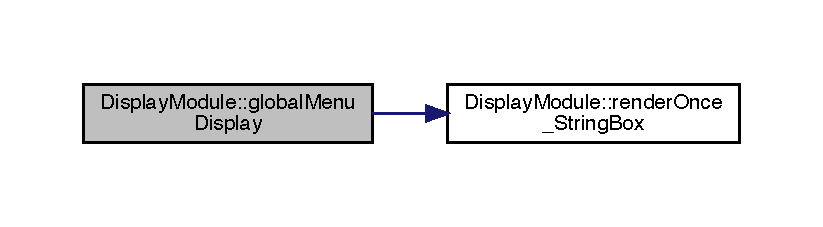
\includegraphics[width=350pt]{class_display_module_a5082cabe11332dc4a9d0daea8a60f9dc_cgraph}
\end{center}
\end{figure}
Here is the caller graph for this function\+:
\nopagebreak
\begin{figure}[H]
\begin{center}
\leavevmode
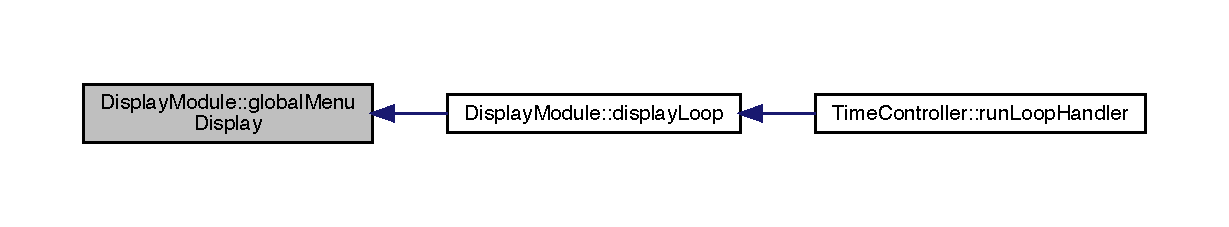
\includegraphics[width=350pt]{class_display_module_a5082cabe11332dc4a9d0daea8a60f9dc_icgraph}
\end{center}
\end{figure}
\mbox{\Hypertarget{class_display_module_a68451c130f98f5d820377e9aa15a7242}\label{class_display_module_a68451c130f98f5d820377e9aa15a7242}} 
\index{Display\+Module@{Display\+Module}!initialize@{initialize}}
\index{initialize@{initialize}!Display\+Module@{Display\+Module}}
\subsubsection{\texorpdfstring{initialize()}{initialize()}}
{\footnotesize\ttfamily void Display\+Module\+::initialize (\begin{DoxyParamCaption}\item[{Sequencer $\ast$}]{sequence\+Array }\end{DoxyParamCaption})}

Here is the caller graph for this function\+:
\nopagebreak
\begin{figure}[H]
\begin{center}
\leavevmode
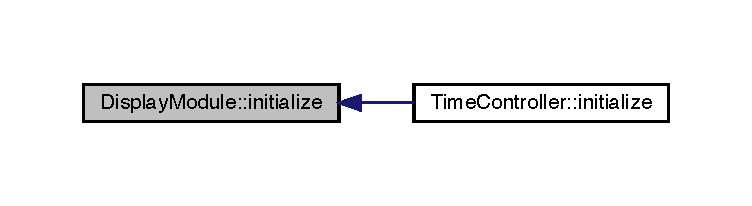
\includegraphics[width=350pt]{class_display_module_a68451c130f98f5d820377e9aa15a7242_icgraph}
\end{center}
\end{figure}
\mbox{\Hypertarget{class_display_module_a776e918a0d9f50ae079d6839524cc471}\label{class_display_module_a776e918a0d9f50ae079d6839524cc471}} 
\index{Display\+Module@{Display\+Module}!input\+Debug\+Menu\+Display@{input\+Debug\+Menu\+Display}}
\index{input\+Debug\+Menu\+Display@{input\+Debug\+Menu\+Display}!Display\+Module@{Display\+Module}}
\subsubsection{\texorpdfstring{input\+Debug\+Menu\+Display()}{inputDebugMenuDisplay()}}
{\footnotesize\ttfamily void Display\+Module\+::input\+Debug\+Menu\+Display (\begin{DoxyParamCaption}{ }\end{DoxyParamCaption})}

Here is the call graph for this function\+:
\nopagebreak
\begin{figure}[H]
\begin{center}
\leavevmode
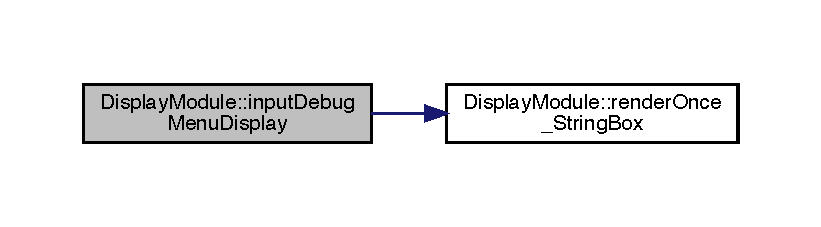
\includegraphics[width=350pt]{class_display_module_a776e918a0d9f50ae079d6839524cc471_cgraph}
\end{center}
\end{figure}
Here is the caller graph for this function\+:
\nopagebreak
\begin{figure}[H]
\begin{center}
\leavevmode
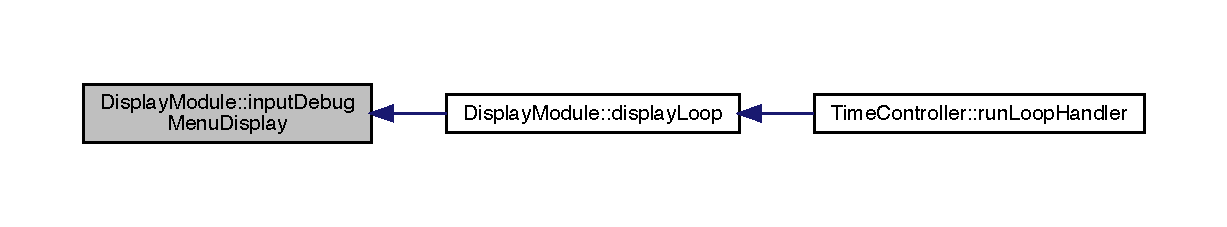
\includegraphics[width=350pt]{class_display_module_a776e918a0d9f50ae079d6839524cc471_icgraph}
\end{center}
\end{figure}
\mbox{\Hypertarget{class_display_module_a95fa96a6b2d74b8d15eeb0c71786b1b2}\label{class_display_module_a95fa96a6b2d74b8d15eeb0c71786b1b2}} 
\index{Display\+Module@{Display\+Module}!pattern\+Select\+Display@{pattern\+Select\+Display}}
\index{pattern\+Select\+Display@{pattern\+Select\+Display}!Display\+Module@{Display\+Module}}
\subsubsection{\texorpdfstring{pattern\+Select\+Display()}{patternSelectDisplay()}}
{\footnotesize\ttfamily void Display\+Module\+::pattern\+Select\+Display (\begin{DoxyParamCaption}{ }\end{DoxyParamCaption})}

Here is the call graph for this function\+:
\nopagebreak
\begin{figure}[H]
\begin{center}
\leavevmode
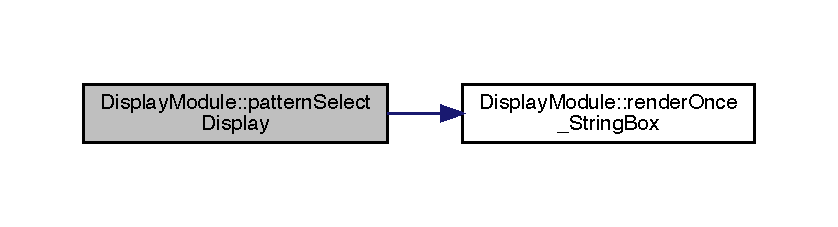
\includegraphics[width=350pt]{class_display_module_a95fa96a6b2d74b8d15eeb0c71786b1b2_cgraph}
\end{center}
\end{figure}
Here is the caller graph for this function\+:
\nopagebreak
\begin{figure}[H]
\begin{center}
\leavevmode
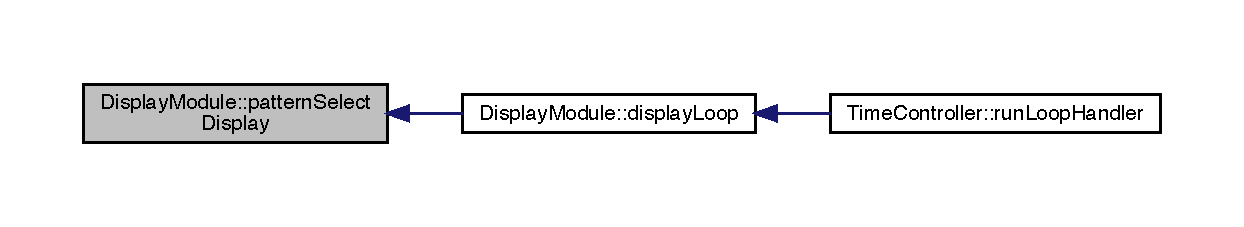
\includegraphics[width=350pt]{class_display_module_a95fa96a6b2d74b8d15eeb0c71786b1b2_icgraph}
\end{center}
\end{figure}
\mbox{\Hypertarget{class_display_module_a453ceefb9e2a9a82dd7b62825cc2cac8}\label{class_display_module_a453ceefb9e2a9a82dd7b62825cc2cac8}} 
\index{Display\+Module@{Display\+Module}!render\+Once\+\_\+\+String\+Box@{render\+Once\+\_\+\+String\+Box}}
\index{render\+Once\+\_\+\+String\+Box@{render\+Once\+\_\+\+String\+Box}!Display\+Module@{Display\+Module}}
\subsubsection{\texorpdfstring{render\+Once\+\_\+\+String\+Box()}{renderOnce\_StringBox()}}
{\footnotesize\ttfamily void Display\+Module\+::render\+Once\+\_\+\+String\+Box (\begin{DoxyParamCaption}\item[{uint8\+\_\+t}]{index,  }\item[{uint8\+\_\+t}]{highlight,  }\item[{uint8\+\_\+t}]{previous\+Highlight,  }\item[{int16\+\_\+t}]{x,  }\item[{int16\+\_\+t}]{y,  }\item[{int16\+\_\+t}]{w,  }\item[{int16\+\_\+t}]{h,  }\item[{bool}]{border,  }\item[{uint8\+\_\+t}]{text\+Size,  }\item[{uint16\+\_\+t}]{color,  }\item[{uint16\+\_\+t}]{bg\+Color }\end{DoxyParamCaption})}

Here is the caller graph for this function\+:
\nopagebreak
\begin{figure}[H]
\begin{center}
\leavevmode
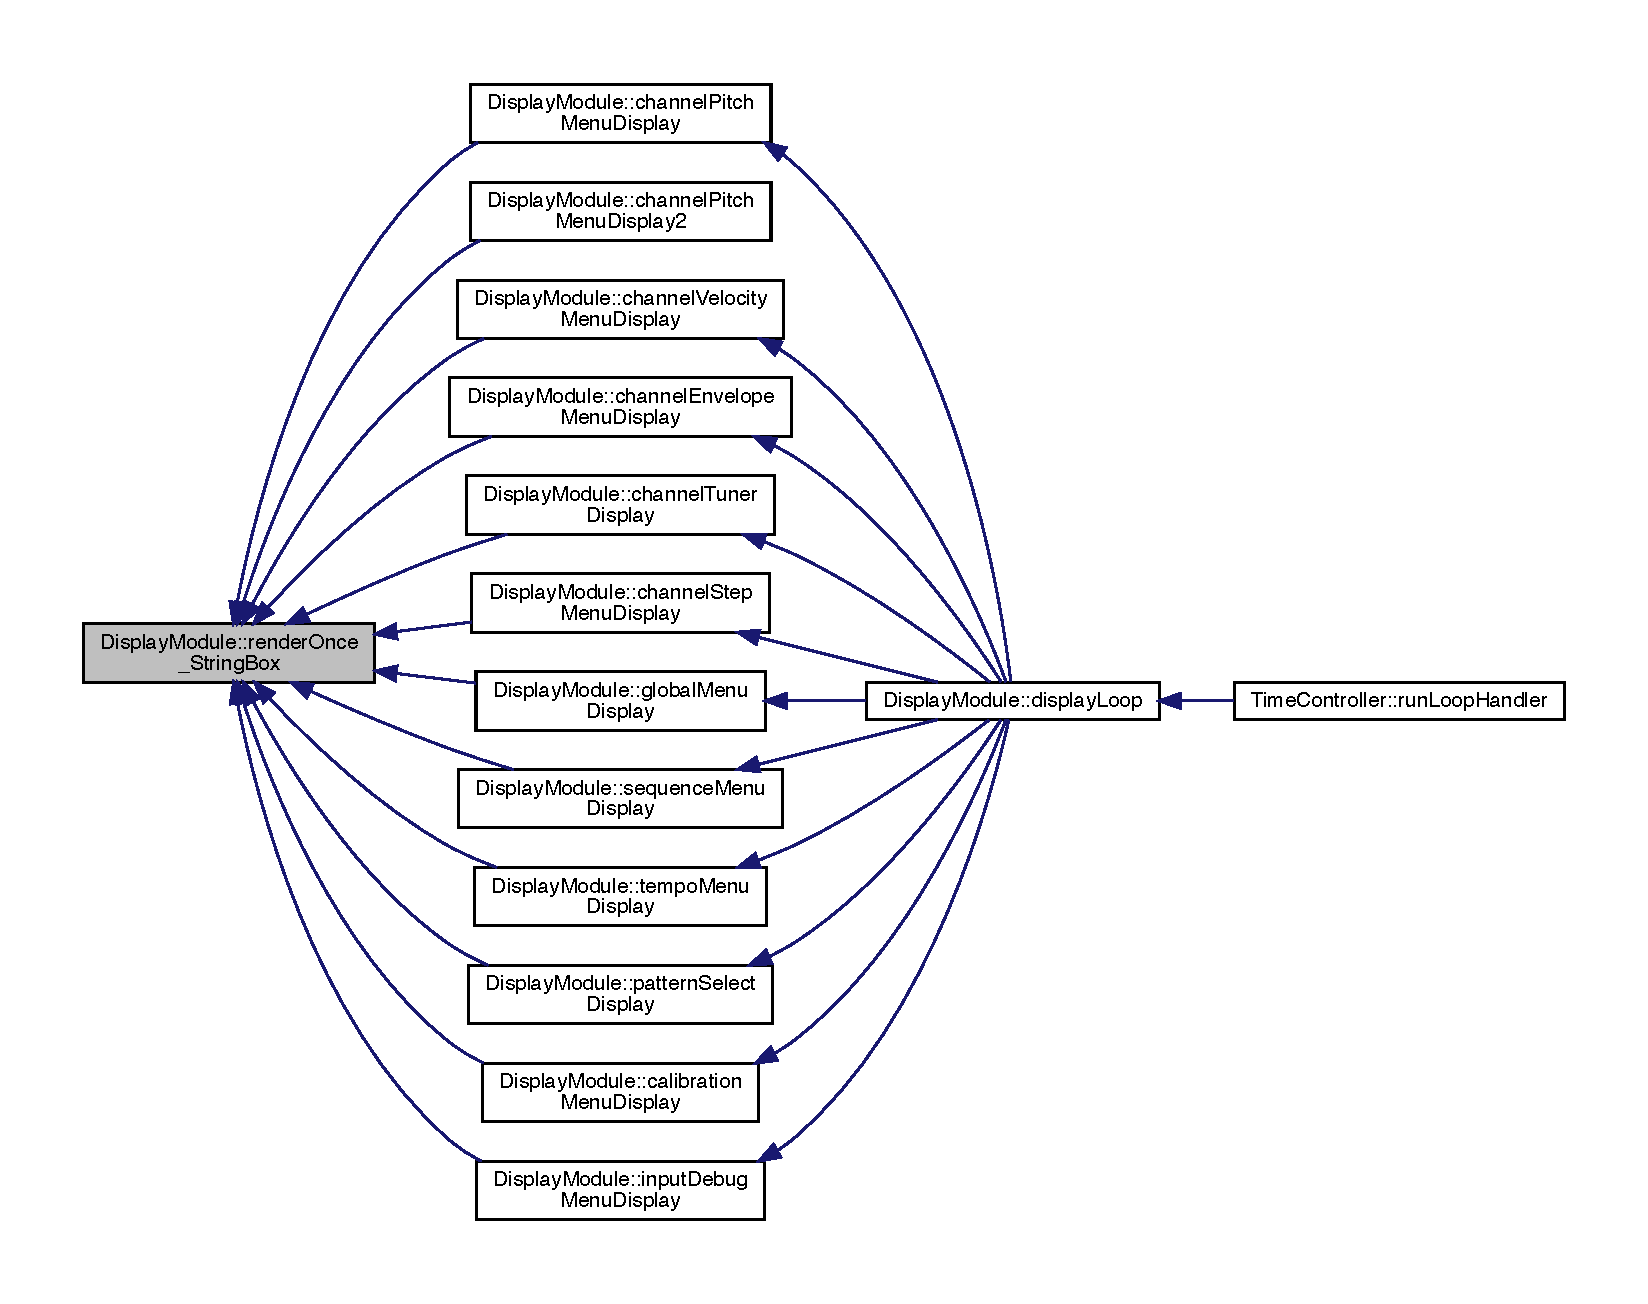
\includegraphics[width=350pt]{class_display_module_a453ceefb9e2a9a82dd7b62825cc2cac8_icgraph}
\end{center}
\end{figure}
\mbox{\Hypertarget{class_display_module_a3e2fc0a60ef41f41e57d463faf59bd2b}\label{class_display_module_a3e2fc0a60ef41f41e57d463faf59bd2b}} 
\index{Display\+Module@{Display\+Module}!sequence\+Menu\+Display@{sequence\+Menu\+Display}}
\index{sequence\+Menu\+Display@{sequence\+Menu\+Display}!Display\+Module@{Display\+Module}}
\subsubsection{\texorpdfstring{sequence\+Menu\+Display()}{sequenceMenuDisplay()}}
{\footnotesize\ttfamily void Display\+Module\+::sequence\+Menu\+Display (\begin{DoxyParamCaption}{ }\end{DoxyParamCaption})}

Here is the call graph for this function\+:
\nopagebreak
\begin{figure}[H]
\begin{center}
\leavevmode
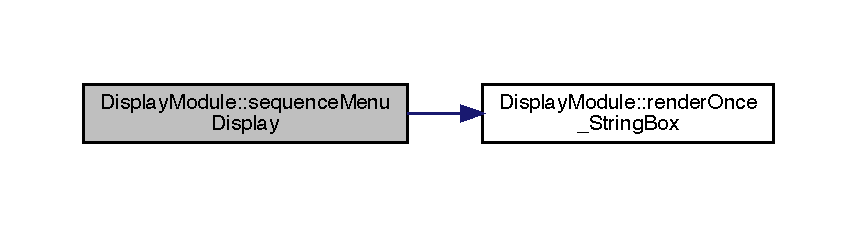
\includegraphics[width=350pt]{class_display_module_a3e2fc0a60ef41f41e57d463faf59bd2b_cgraph}
\end{center}
\end{figure}
Here is the caller graph for this function\+:
\nopagebreak
\begin{figure}[H]
\begin{center}
\leavevmode
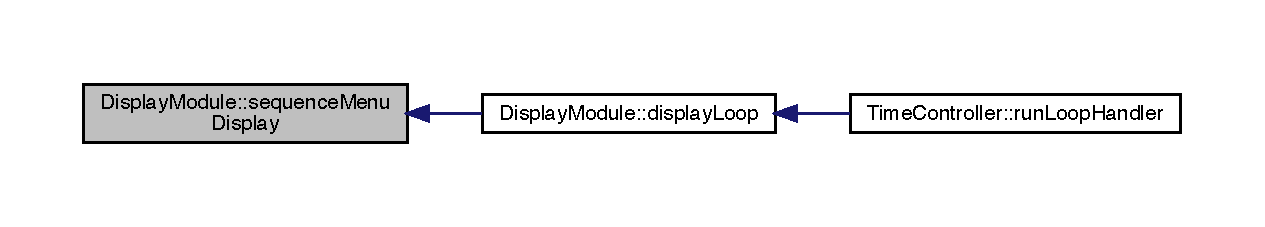
\includegraphics[width=350pt]{class_display_module_a3e2fc0a60ef41f41e57d463faf59bd2b_icgraph}
\end{center}
\end{figure}
\mbox{\Hypertarget{class_display_module_ac1d55595826fc36738b2d9df6be9516e}\label{class_display_module_ac1d55595826fc36738b2d9df6be9516e}} 
\index{Display\+Module@{Display\+Module}!step\+Display@{step\+Display}}
\index{step\+Display@{step\+Display}!Display\+Module@{Display\+Module}}
\subsubsection{\texorpdfstring{step\+Display()}{stepDisplay()}}
{\footnotesize\ttfamily void Display\+Module\+::step\+Display (\begin{DoxyParamCaption}\item[{char $\ast$}]{buf }\end{DoxyParamCaption})}

\mbox{\Hypertarget{class_display_module_ac5999c2f0f4b1ecc12bafe7094c7b7d2}\label{class_display_module_ac5999c2f0f4b1ecc12bafe7094c7b7d2}} 
\index{Display\+Module@{Display\+Module}!tempo\+Menu\+Display@{tempo\+Menu\+Display}}
\index{tempo\+Menu\+Display@{tempo\+Menu\+Display}!Display\+Module@{Display\+Module}}
\subsubsection{\texorpdfstring{tempo\+Menu\+Display()}{tempoMenuDisplay()}}
{\footnotesize\ttfamily void Display\+Module\+::tempo\+Menu\+Display (\begin{DoxyParamCaption}{ }\end{DoxyParamCaption})}

Here is the call graph for this function\+:
\nopagebreak
\begin{figure}[H]
\begin{center}
\leavevmode
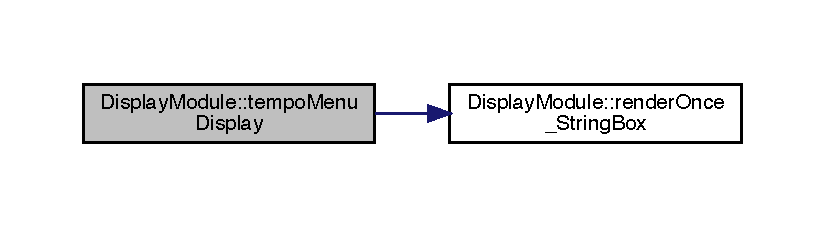
\includegraphics[width=350pt]{class_display_module_ac5999c2f0f4b1ecc12bafe7094c7b7d2_cgraph}
\end{center}
\end{figure}
Here is the caller graph for this function\+:
\nopagebreak
\begin{figure}[H]
\begin{center}
\leavevmode
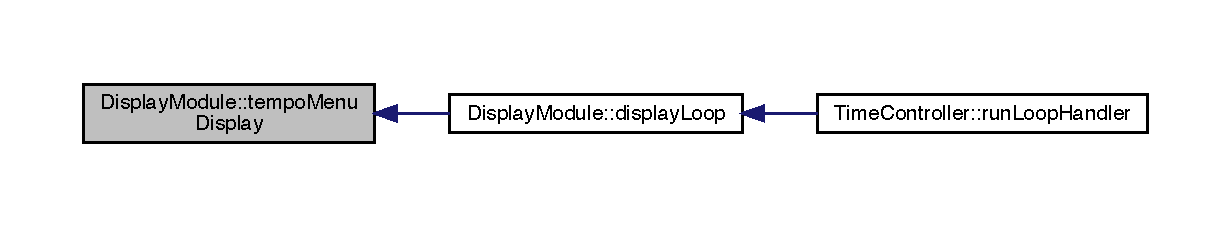
\includegraphics[width=350pt]{class_display_module_ac5999c2f0f4b1ecc12bafe7094c7b7d2_icgraph}
\end{center}
\end{figure}
\mbox{\Hypertarget{class_display_module_a722a8c3b1cce1c58fa7e17e2865c3e57}\label{class_display_module_a722a8c3b1cce1c58fa7e17e2865c3e57}} 
\index{Display\+Module@{Display\+Module}!timing\+Menu\+Display@{timing\+Menu\+Display}}
\index{timing\+Menu\+Display@{timing\+Menu\+Display}!Display\+Module@{Display\+Module}}
\subsubsection{\texorpdfstring{timing\+Menu\+Display()}{timingMenuDisplay()}}
{\footnotesize\ttfamily void Display\+Module\+::timing\+Menu\+Display (\begin{DoxyParamCaption}{ }\end{DoxyParamCaption})}

Here is the caller graph for this function\+:
\nopagebreak
\begin{figure}[H]
\begin{center}
\leavevmode
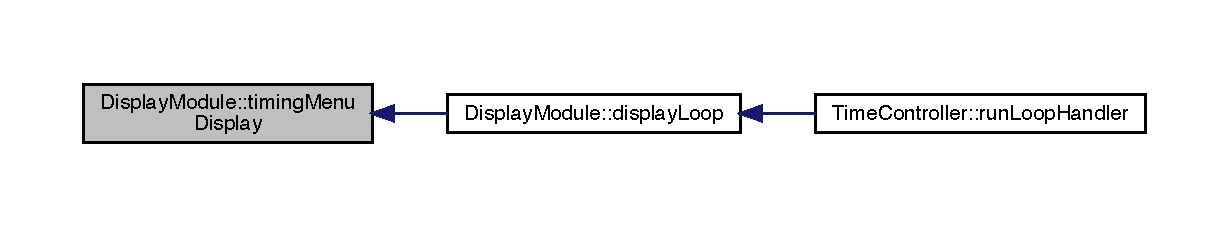
\includegraphics[width=350pt]{class_display_module_a722a8c3b1cce1c58fa7e17e2865c3e57_icgraph}
\end{center}
\end{figure}


\subsection{Member Data Documentation}
\mbox{\Hypertarget{class_display_module_a7ebe1c30eb4c306a99a3129f6a165e2a}\label{class_display_module_a7ebe1c30eb4c306a99a3129f6a165e2a}} 
\index{Display\+Module@{Display\+Module}!background@{background}}
\index{background@{background}!Display\+Module@{Display\+Module}}
\subsubsection{\texorpdfstring{background}{background}}
{\footnotesize\ttfamily uint16\+\_\+t Display\+Module\+::background}

\mbox{\Hypertarget{class_display_module_a07c140067fde1f0cbc4061296179d69a}\label{class_display_module_a07c140067fde1f0cbc4061296179d69a}} 
\index{Display\+Module@{Display\+Module}!buf@{buf}}
\index{buf@{buf}!Display\+Module@{Display\+Module}}
\subsubsection{\texorpdfstring{buf}{buf}}
{\footnotesize\ttfamily char$\ast$ Display\+Module\+::buf = new char\mbox{[}51\mbox{]}}

\mbox{\Hypertarget{class_display_module_ac071b7f3b2027d0e90b7d3031d61a99b}\label{class_display_module_ac071b7f3b2027d0e90b7d3031d61a99b}} 
\index{Display\+Module@{Display\+Module}!color@{color}}
\index{color@{color}!Display\+Module@{Display\+Module}}
\subsubsection{\texorpdfstring{color}{color}}
{\footnotesize\ttfamily int Display\+Module\+::color = 0}

\mbox{\Hypertarget{class_display_module_adf0d12d4d19fa7bff2fc66411e4255a2}\label{class_display_module_adf0d12d4d19fa7bff2fc66411e4255a2}} 
\index{Display\+Module@{Display\+Module}!display\+Cache@{display\+Cache}}
\index{display\+Cache@{display\+Cache}!Display\+Module@{Display\+Module}}
\subsubsection{\texorpdfstring{display\+Cache}{displayCache}}
{\footnotesize\ttfamily char$\ast$ Display\+Module\+::display\+Cache\mbox{[}\hyperlink{display_module_8h_a6114392da1243b69a45b549bd4ddfd39}{M\+A\+X\+\_\+\+D\+I\+S\+P\+L\+A\+Y\+\_\+\+E\+L\+E\+M\+E\+N\+TS}\mbox{]}}

\mbox{\Hypertarget{class_display_module_a7af82afb24a27ab297fda02a9d1f0eb3}\label{class_display_module_a7af82afb24a27ab297fda02a9d1f0eb3}} 
\index{Display\+Module@{Display\+Module}!display\+Element@{display\+Element}}
\index{display\+Element@{display\+Element}!Display\+Module@{Display\+Module}}
\subsubsection{\texorpdfstring{display\+Element}{displayElement}}
{\footnotesize\ttfamily char$\ast$ Display\+Module\+::display\+Element\mbox{[}\hyperlink{display_module_8h_a6114392da1243b69a45b549bd4ddfd39}{M\+A\+X\+\_\+\+D\+I\+S\+P\+L\+A\+Y\+\_\+\+E\+L\+E\+M\+E\+N\+TS}\mbox{]}}

\mbox{\Hypertarget{class_display_module_a0c92fa8b35e030ef848db6207fe5067b}\label{class_display_module_a0c92fa8b35e030ef848db6207fe5067b}} 
\index{Display\+Module@{Display\+Module}!display\+Timer@{display\+Timer}}
\index{display\+Timer@{display\+Timer}!Display\+Module@{Display\+Module}}
\subsubsection{\texorpdfstring{display\+Timer}{displayTimer}}
{\footnotesize\ttfamily elapsed\+Micros Display\+Module\+::display\+Timer}

\mbox{\Hypertarget{class_display_module_ab3b6b57d36f08a63a68641eefdb56446}\label{class_display_module_ab3b6b57d36f08a63a68641eefdb56446}} 
\index{Display\+Module@{Display\+Module}!foreground@{foreground}}
\index{foreground@{foreground}!Display\+Module@{Display\+Module}}
\subsubsection{\texorpdfstring{foreground}{foreground}}
{\footnotesize\ttfamily uint16\+\_\+t Display\+Module\+::foreground}

\mbox{\Hypertarget{class_display_module_a33ee7436481d6285fb6c81166711fbce}\label{class_display_module_a33ee7436481d6285fb6c81166711fbce}} 
\index{Display\+Module@{Display\+Module}!highlight@{highlight}}
\index{highlight@{highlight}!Display\+Module@{Display\+Module}}
\subsubsection{\texorpdfstring{highlight}{highlight}}
{\footnotesize\ttfamily uint8\+\_\+t Display\+Module\+::highlight}

\mbox{\Hypertarget{class_display_module_a76bde3057832542df04f4796ae917d48}\label{class_display_module_a76bde3057832542df04f4796ae917d48}} 
\index{Display\+Module@{Display\+Module}!midi\+Notes@{midi\+Notes}}
\index{midi\+Notes@{midi\+Notes}!Display\+Module@{Display\+Module}}
\subsubsection{\texorpdfstring{midi\+Notes}{midiNotes}}
{\footnotesize\ttfamily const char$\ast$ Display\+Module\+::midi\+Notes\mbox{[}128\mbox{]}\hspace{0.3cm}{\ttfamily [private]}}

{\bfseries Initial value\+:}
\begin{DoxyCode}
= \{
    \textcolor{stringliteral}{"C -2"},\textcolor{stringliteral}{"C#-2"},\textcolor{stringliteral}{"D -2"},\textcolor{stringliteral}{"D#-2"},\textcolor{stringliteral}{"E -2"},\textcolor{stringliteral}{"F -2"},\textcolor{stringliteral}{"F#-2"},\textcolor{stringliteral}{"G -2"},\textcolor{stringliteral}{"G#-2"},\textcolor{stringliteral}{"A -2"},\textcolor{stringliteral}{"A#-2"},\textcolor{stringliteral}{"B -2"},
    \textcolor{stringliteral}{"C -1"},\textcolor{stringliteral}{"C#-1"},\textcolor{stringliteral}{"D -1"},\textcolor{stringliteral}{"D#-1"},\textcolor{stringliteral}{"E -1"},\textcolor{stringliteral}{"F -1"},\textcolor{stringliteral}{"F#-1"},\textcolor{stringliteral}{"G -1"},\textcolor{stringliteral}{"G#-1"},\textcolor{stringliteral}{"A -1"},\textcolor{stringliteral}{"A#-1"},\textcolor{stringliteral}{"B -1"},
    \textcolor{stringliteral}{"C  0"},\textcolor{stringliteral}{"C# 0"},\textcolor{stringliteral}{"D  0"},\textcolor{stringliteral}{"D# 0"},\textcolor{stringliteral}{"E  0"},\textcolor{stringliteral}{"F  0"},\textcolor{stringliteral}{"F# 0"},\textcolor{stringliteral}{"G  0"},\textcolor{stringliteral}{"G# 0"},\textcolor{stringliteral}{"A  0"},\textcolor{stringliteral}{"A# 0"},\textcolor{stringliteral}{"B  0"},
    \textcolor{stringliteral}{"C  1"},\textcolor{stringliteral}{"C# 1"},\textcolor{stringliteral}{"D  1"},\textcolor{stringliteral}{"D# 1"},\textcolor{stringliteral}{"E  1"},\textcolor{stringliteral}{"F  1"},\textcolor{stringliteral}{"F# 1"},\textcolor{stringliteral}{"G  1"},\textcolor{stringliteral}{"G# 1"},\textcolor{stringliteral}{"A  1"},\textcolor{stringliteral}{"A# 1"},\textcolor{stringliteral}{"B  1"},
    \textcolor{stringliteral}{"C  2"},\textcolor{stringliteral}{"C# 2"},\textcolor{stringliteral}{"D  2"},\textcolor{stringliteral}{"D# 2"},\textcolor{stringliteral}{"E  2"},\textcolor{stringliteral}{"F  2"},\textcolor{stringliteral}{"F# 2"},\textcolor{stringliteral}{"G  2"},\textcolor{stringliteral}{"G# 2"},\textcolor{stringliteral}{"A  2"},\textcolor{stringliteral}{"A# 2"},\textcolor{stringliteral}{"B  2"},
    \textcolor{stringliteral}{"C  3"},\textcolor{stringliteral}{"C# 3"},\textcolor{stringliteral}{"D  3"},\textcolor{stringliteral}{"D# 3"},\textcolor{stringliteral}{"E  3"},\textcolor{stringliteral}{"F  3"},\textcolor{stringliteral}{"F# 3"},\textcolor{stringliteral}{"G  3"},\textcolor{stringliteral}{"G# 3"},\textcolor{stringliteral}{"A  3"},\textcolor{stringliteral}{"A# 3"},\textcolor{stringliteral}{"B  3"},
    \textcolor{stringliteral}{"C  4"},\textcolor{stringliteral}{"C# 4"},\textcolor{stringliteral}{"D  4"},\textcolor{stringliteral}{"D# 4"},\textcolor{stringliteral}{"E  4"},\textcolor{stringliteral}{"F  4"},\textcolor{stringliteral}{"F# 4"},\textcolor{stringliteral}{"G  4"},\textcolor{stringliteral}{"G# 4"},\textcolor{stringliteral}{"A  4"},\textcolor{stringliteral}{"A# 4"},\textcolor{stringliteral}{"B  4"},
    \textcolor{stringliteral}{"C  5"},\textcolor{stringliteral}{"C# 5"},\textcolor{stringliteral}{"D  5"},\textcolor{stringliteral}{"D# 5"},\textcolor{stringliteral}{"E  5"},\textcolor{stringliteral}{"F  5"},\textcolor{stringliteral}{"F# 5"},\textcolor{stringliteral}{"G  5"},\textcolor{stringliteral}{"G# 5"},\textcolor{stringliteral}{"A  5"},\textcolor{stringliteral}{"A# 5"},\textcolor{stringliteral}{"B  5"},
    \textcolor{stringliteral}{"C  6"},\textcolor{stringliteral}{"C# 6"},\textcolor{stringliteral}{"D  6"},\textcolor{stringliteral}{"D# 6"},\textcolor{stringliteral}{"E  6"},\textcolor{stringliteral}{"F  6"},\textcolor{stringliteral}{"F# 6"},\textcolor{stringliteral}{"G  6"},\textcolor{stringliteral}{"G# 6"},\textcolor{stringliteral}{"A  6"},\textcolor{stringliteral}{"A# 6"},\textcolor{stringliteral}{"B  6"},
    \textcolor{stringliteral}{"C  7"},\textcolor{stringliteral}{"C# 7"},\textcolor{stringliteral}{"D  7"},\textcolor{stringliteral}{"D# 7"},\textcolor{stringliteral}{"E  7"},\textcolor{stringliteral}{"F  7"},\textcolor{stringliteral}{"F# 7"},\textcolor{stringliteral}{"G  7"},\textcolor{stringliteral}{"G# 7"},\textcolor{stringliteral}{"A  7"},\textcolor{stringliteral}{"A# 7"},\textcolor{stringliteral}{"B  7"},
    \textcolor{stringliteral}{"C  8"},\textcolor{stringliteral}{"C# 8"},\textcolor{stringliteral}{"D  8"},\textcolor{stringliteral}{"D# 8"},\textcolor{stringliteral}{"E  8"},\textcolor{stringliteral}{"F  8"},\textcolor{stringliteral}{"F# 8"},\textcolor{stringliteral}{"G  8"} \}
\end{DoxyCode}
\mbox{\Hypertarget{class_display_module_abcfa732c08671b60dbf7f8d7e0d17e74}\label{class_display_module_abcfa732c08671b60dbf7f8d7e0d17e74}} 
\index{Display\+Module@{Display\+Module}!oled@{oled}}
\index{oled@{oled}!Display\+Module@{Display\+Module}}
\subsubsection{\texorpdfstring{oled}{oled}}
{\footnotesize\ttfamily S\+S\+D\+\_\+13\+XX Display\+Module\+::oled = S\+S\+D\+\_\+13\+XX(\hyperlink{display_module_8h_a71d24cab0e16b054de228f29139f1b79}{L\+C\+D\+\_\+\+CS}, \hyperlink{display_module_8h_a1dc6c4886242abf4447d0da651125d5d}{L\+C\+D\+\_\+\+DC}, \hyperlink{display_module_8h_aec0f0ab242f1b58b1d017bc9ab4b898b}{L\+C\+D\+\_\+\+R\+ST})}

\mbox{\Hypertarget{class_display_module_aaca9b1f6821215e5ebdc5bb6edb390b8}\label{class_display_module_aaca9b1f6821215e5ebdc5bb6edb390b8}} 
\index{Display\+Module@{Display\+Module}!previously\+Selected\+Channel@{previously\+Selected\+Channel}}
\index{previously\+Selected\+Channel@{previously\+Selected\+Channel}!Display\+Module@{Display\+Module}}
\subsubsection{\texorpdfstring{previously\+Selected\+Channel}{previouslySelectedChannel}}
{\footnotesize\ttfamily uint8\+\_\+t Display\+Module\+::previously\+Selected\+Channel}

\mbox{\Hypertarget{class_display_module_a5c8825161e8df40668c79145e5dace28}\label{class_display_module_a5c8825161e8df40668c79145e5dace28}} 
\index{Display\+Module@{Display\+Module}!runcount@{runcount}}
\index{runcount@{runcount}!Display\+Module@{Display\+Module}}
\subsubsection{\texorpdfstring{runcount}{runcount}}
{\footnotesize\ttfamily uint32\+\_\+t Display\+Module\+::runcount}

\mbox{\Hypertarget{class_display_module_a9eb0f63acb02bc366bdc36cf60efb799}\label{class_display_module_a9eb0f63acb02bc366bdc36cf60efb799}} 
\index{Display\+Module@{Display\+Module}!sequence\+Array@{sequence\+Array}}
\index{sequence\+Array@{sequence\+Array}!Display\+Module@{Display\+Module}}
\subsubsection{\texorpdfstring{sequence\+Array}{sequenceArray}}
{\footnotesize\ttfamily Sequencer$\ast$ Display\+Module\+::sequence\+Array\hspace{0.3cm}{\ttfamily [private]}}



The documentation for this class was generated from the following files\+:\begin{DoxyCompactItemize}
\item 
src/\hyperlink{display_module_8h}{display\+Module.\+h}\item 
src/\hyperlink{display_module_8cpp}{display\+Module.\+cpp}\end{DoxyCompactItemize}

\hypertarget{class_input_module}{}\section{Input\+Module Class Reference}
\label{class_input_module}\index{Input\+Module@{Input\+Module}}


{\ttfamily \#include $<$input\+Module.\+h$>$}



Collaboration diagram for Input\+Module\+:
\nopagebreak
\begin{figure}[H]
\begin{center}
\leavevmode
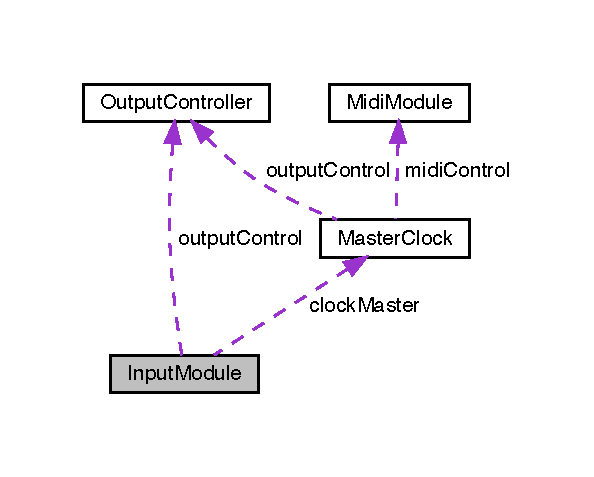
\includegraphics[width=285pt]{class_input_module__coll__graph}
\end{center}
\end{figure}
\subsection*{Public Member Functions}
\begin{DoxyCompactItemize}
\item 
\hyperlink{class_input_module_a158c97df320462df4e6986be5a2b2646}{Input\+Module} ()
\item 
void \hyperlink{class_input_module_a789c6f0da21e6b5b89c7c6991f4ee745}{initialize} (\hyperlink{class_output_controller}{Output\+Controller} $\ast$\hyperlink{class_input_module_ad1019ec5aac3175710630718e056e471}{output\+Control}, Zetaohm\+\_\+\+M\+A\+X7301 $\ast$\hyperlink{class_input_module_ad23720995ebd07355df926bb18e2260d}{midplane\+G\+P\+IO}, Zetaohm\+\_\+\+M\+A\+X7301 $\ast$\hyperlink{class_input_module_a433abde922dee6f2abed80710f49a294}{backplane\+G\+P\+IO}, Flash\+Memory $\ast$\hyperlink{class_input_module_a0a4fbca5f978a217f47ed31082eaaecc}{save\+File}, Sequencer $\ast$\hyperlink{class_input_module_afdc54a8219ed5b5743201a00efd2cb72}{sequence\+Array}, \hyperlink{class_master_clock}{Master\+Clock} $\ast$\hyperlink{class_input_module_aff739621e5d47367263551f43d98b94b}{clock\+Master})
\item 
void \hyperlink{class_input_module_ad481ab7241ffe3a168e063a5afd6d892}{loop} (uint16\+\_\+t \hyperlink{global_8h_acdfc8898c9e67fbcec81f3b04ae61bd9}{frequency})
\item 
void \hyperlink{class_input_module_a92fa77f3667cbfdce6c2fbdc14854811}{pattern\+Select\+Handler} ()
\item 
void \hyperlink{class_input_module_a62ad05f2e4880aeae014d99ecfcd494d}{channel\+Button\+Handler} (uint8\+\_\+t channel)
\item 
void \hyperlink{class_input_module_a2e678e1a6f2d7b9f91a6e6f1e3125e89}{channel\+Button\+Shift\+Handler} (uint8\+\_\+t channel)
\item 
void \hyperlink{class_input_module_a1f93d0b1fc3269147f4d03a888ddb631}{alt\+Button\+Handler} ()
\item 
void \hyperlink{class_input_module_ada290dc92f0ad59826c47781ea2209c0}{step\+Mode\+Matrix\+Handler} ()
\item 
void \hyperlink{class_input_module_af8193a3e5f84adb8a139d624742b8c6a}{channel\+Pitch\+Mode\+Input\+Handler} ()
\item 
void \hyperlink{class_input_module_a30c140bcc298b2c7c382ef290e77071f}{channel\+Velocity\+Mode\+Input\+Handler} ()
\item 
void \hyperlink{class_input_module_a0ff214fef897f5dd0bd0384673742996}{channel\+Envelope\+Mode\+Input\+Handler} ()
\item 
void \hyperlink{class_input_module_ae5323fd937a03aff47a5696c67ca87d2}{channel\+Step\+Mode\+Input\+Handler} ()
\item 
void \hyperlink{class_input_module_a6b0c9027e4088393722d00d162e4ecd9}{sequence\+Menu\+Handler} ()
\item 
void \hyperlink{class_input_module_a9844fa2022c8e526c431cd084556ffe0}{global\+Menu\+Handler} ()
\item 
void \hyperlink{class_input_module_a2e71a13d6f8365f5753fae8f4542769c}{tempo\+Menu\+Handler} ()
\item 
void \hyperlink{class_input_module_ab5048e031568fa6879b6618e4478cc97}{timing\+Menu\+Input\+Handler} ()
\item 
void \hyperlink{class_input_module_a341016de304d4ac105a9f5c98a76a853}{debug\+Screen\+Input\+Handler} ()
\item 
void \hyperlink{class_input_module_a75dd14eb87936e206ba74ca406851201}{calibration\+Menu\+Handler} ()
\item 
void \hyperlink{class_input_module_a1bbac8d8d543c1adfdaa955f251db63a}{reset\+Knob\+Values} ()
\item 
void \hyperlink{class_input_module_ac6242c4331441ba020d2fca7bff7a401}{change\+State} (uint8\+\_\+t state)
\end{DoxyCompactItemize}
\subsection*{Public Attributes}
\begin{DoxyCompactItemize}
\item 
Encoder \hyperlink{class_input_module_a70e9413a995052805e5c1e6962e1ec46}{knob}
\item 
Zetaohm\+\_\+\+M\+A\+X7301 $\ast$ \hyperlink{class_input_module_ad23720995ebd07355df926bb18e2260d}{midplane\+G\+P\+IO}
\item 
Zetaohm\+\_\+\+M\+A\+X7301 $\ast$ \hyperlink{class_input_module_a433abde922dee6f2abed80710f49a294}{backplane\+G\+P\+IO}
\item 
\hyperlink{class_output_controller}{Output\+Controller} $\ast$ \hyperlink{class_input_module_ad1019ec5aac3175710630718e056e471}{output\+Control}
\item 
\hyperlink{class_master_clock}{Master\+Clock} $\ast$ \hyperlink{class_input_module_aff739621e5d47367263551f43d98b94b}{clock\+Master}
\item 
int8\+\_\+t \hyperlink{class_input_module_a0d7bca8e1d85982108bc2b1c8a9a41fd}{knob\+Read}
\item 
int8\+\_\+t \hyperlink{class_input_module_a6015af9178f42735dd65a308fd132cea}{knob\+Buffer}
\item 
int8\+\_\+t \hyperlink{class_input_module_ad66cbf5057aa15d9428ddb0a6936543a}{knob\+Previous}
\item 
int8\+\_\+t \hyperlink{class_input_module_aa71dde7943b36a879ea305285c042e09}{knob\+Change}
\item 
int8\+\_\+t \hyperlink{class_input_module_a0116c65513c2c09f3e09cdf55e55c4cd}{menu\+Selector}
\item 
int8\+\_\+t \hyperlink{class_input_module_af11a3cf014306369d13bc79c3f5e1bcb}{inst\+Buffer}
\item 
int16\+\_\+t \hyperlink{class_input_module_a0197f1734ab95dd812a7747c9c2374b5}{step\+Mode\+Buffer}
\item 
unsigned long \hyperlink{class_input_module_a8479fea0b1f501250aa5026844d6a1a9}{encoder\+Loop\+Time}
\item 
unsigned long \hyperlink{class_input_module_ad8ba561dc4d0372e46a5b8a0e0eb82d9}{small\+Button\+Loop\+Time}
\item 
unsigned long \hyperlink{class_input_module_a56b62ba8836c0fb6ed93ca126bf9a02d}{encoder\+Button\+Time}
\item 
unsigned long \hyperlink{class_input_module_ae4cc83ddf8ca352a05aef5d737e57bc1}{matrix\+Button\+Time}
\end{DoxyCompactItemize}
\subsection*{Private Attributes}
\begin{DoxyCompactItemize}
\item 
Sequencer $\ast$ \hyperlink{class_input_module_afdc54a8219ed5b5743201a00efd2cb72}{sequence\+Array}
\item 
Flash\+Memory $\ast$ \hyperlink{class_input_module_a0a4fbca5f978a217f47ed31082eaaecc}{save\+File}
\item 
elapsed\+Micros \hyperlink{class_input_module_ae0efc931ea904dda2e5b29f8c20181eb}{input\+Timer}
\end{DoxyCompactItemize}


\subsection{Constructor \& Destructor Documentation}
\mbox{\Hypertarget{class_input_module_a158c97df320462df4e6986be5a2b2646}\label{class_input_module_a158c97df320462df4e6986be5a2b2646}} 
\index{Input\+Module@{Input\+Module}!Input\+Module@{Input\+Module}}
\index{Input\+Module@{Input\+Module}!Input\+Module@{Input\+Module}}
\subsubsection{\texorpdfstring{Input\+Module()}{InputModule()}}
{\footnotesize\ttfamily Input\+Module\+::\+Input\+Module (\begin{DoxyParamCaption}{ }\end{DoxyParamCaption})}



\subsection{Member Function Documentation}
\mbox{\Hypertarget{class_input_module_a1f93d0b1fc3269147f4d03a888ddb631}\label{class_input_module_a1f93d0b1fc3269147f4d03a888ddb631}} 
\index{Input\+Module@{Input\+Module}!alt\+Button\+Handler@{alt\+Button\+Handler}}
\index{alt\+Button\+Handler@{alt\+Button\+Handler}!Input\+Module@{Input\+Module}}
\subsubsection{\texorpdfstring{alt\+Button\+Handler()}{altButtonHandler()}}
{\footnotesize\ttfamily void Input\+Module\+::alt\+Button\+Handler (\begin{DoxyParamCaption}{ }\end{DoxyParamCaption})}

Here is the call graph for this function\+:
\nopagebreak
\begin{figure}[H]
\begin{center}
\leavevmode
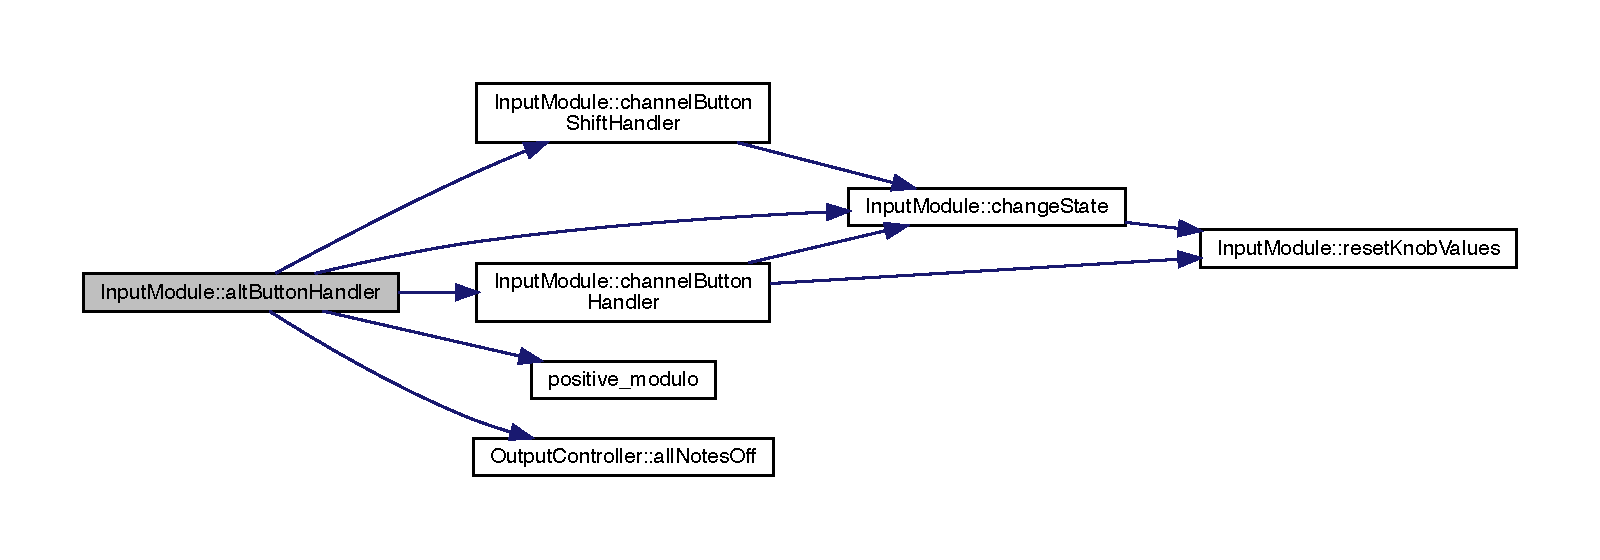
\includegraphics[width=350pt]{class_input_module_a1f93d0b1fc3269147f4d03a888ddb631_cgraph}
\end{center}
\end{figure}
Here is the caller graph for this function\+:
\nopagebreak
\begin{figure}[H]
\begin{center}
\leavevmode
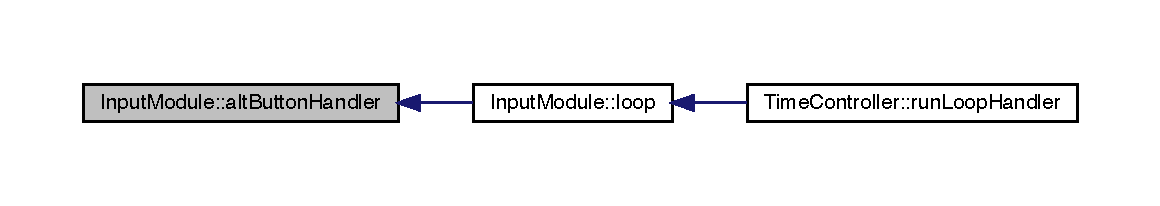
\includegraphics[width=350pt]{class_input_module_a1f93d0b1fc3269147f4d03a888ddb631_icgraph}
\end{center}
\end{figure}
\mbox{\Hypertarget{class_input_module_a75dd14eb87936e206ba74ca406851201}\label{class_input_module_a75dd14eb87936e206ba74ca406851201}} 
\index{Input\+Module@{Input\+Module}!calibration\+Menu\+Handler@{calibration\+Menu\+Handler}}
\index{calibration\+Menu\+Handler@{calibration\+Menu\+Handler}!Input\+Module@{Input\+Module}}
\subsubsection{\texorpdfstring{calibration\+Menu\+Handler()}{calibrationMenuHandler()}}
{\footnotesize\ttfamily void Input\+Module\+::calibration\+Menu\+Handler (\begin{DoxyParamCaption}{ }\end{DoxyParamCaption})}

Here is the call graph for this function\+:
\nopagebreak
\begin{figure}[H]
\begin{center}
\leavevmode
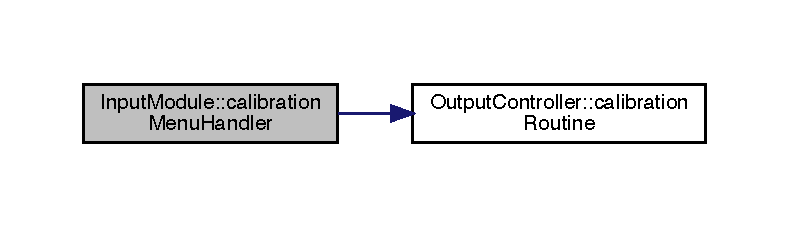
\includegraphics[width=350pt]{class_input_module_a75dd14eb87936e206ba74ca406851201_cgraph}
\end{center}
\end{figure}
Here is the caller graph for this function\+:
\nopagebreak
\begin{figure}[H]
\begin{center}
\leavevmode
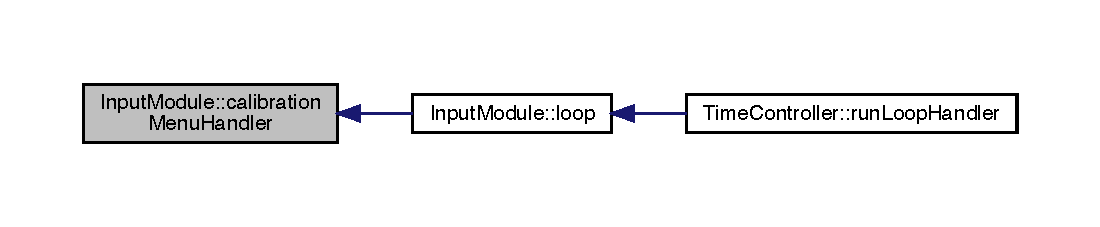
\includegraphics[width=350pt]{class_input_module_a75dd14eb87936e206ba74ca406851201_icgraph}
\end{center}
\end{figure}
\mbox{\Hypertarget{class_input_module_ac6242c4331441ba020d2fca7bff7a401}\label{class_input_module_ac6242c4331441ba020d2fca7bff7a401}} 
\index{Input\+Module@{Input\+Module}!change\+State@{change\+State}}
\index{change\+State@{change\+State}!Input\+Module@{Input\+Module}}
\subsubsection{\texorpdfstring{change\+State()}{changeState()}}
{\footnotesize\ttfamily void Input\+Module\+::change\+State (\begin{DoxyParamCaption}\item[{uint8\+\_\+t}]{state }\end{DoxyParamCaption})}

Here is the call graph for this function\+:
\nopagebreak
\begin{figure}[H]
\begin{center}
\leavevmode
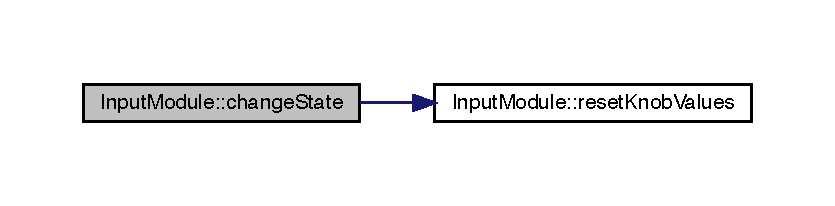
\includegraphics[width=350pt]{class_input_module_ac6242c4331441ba020d2fca7bff7a401_cgraph}
\end{center}
\end{figure}
Here is the caller graph for this function\+:
\nopagebreak
\begin{figure}[H]
\begin{center}
\leavevmode
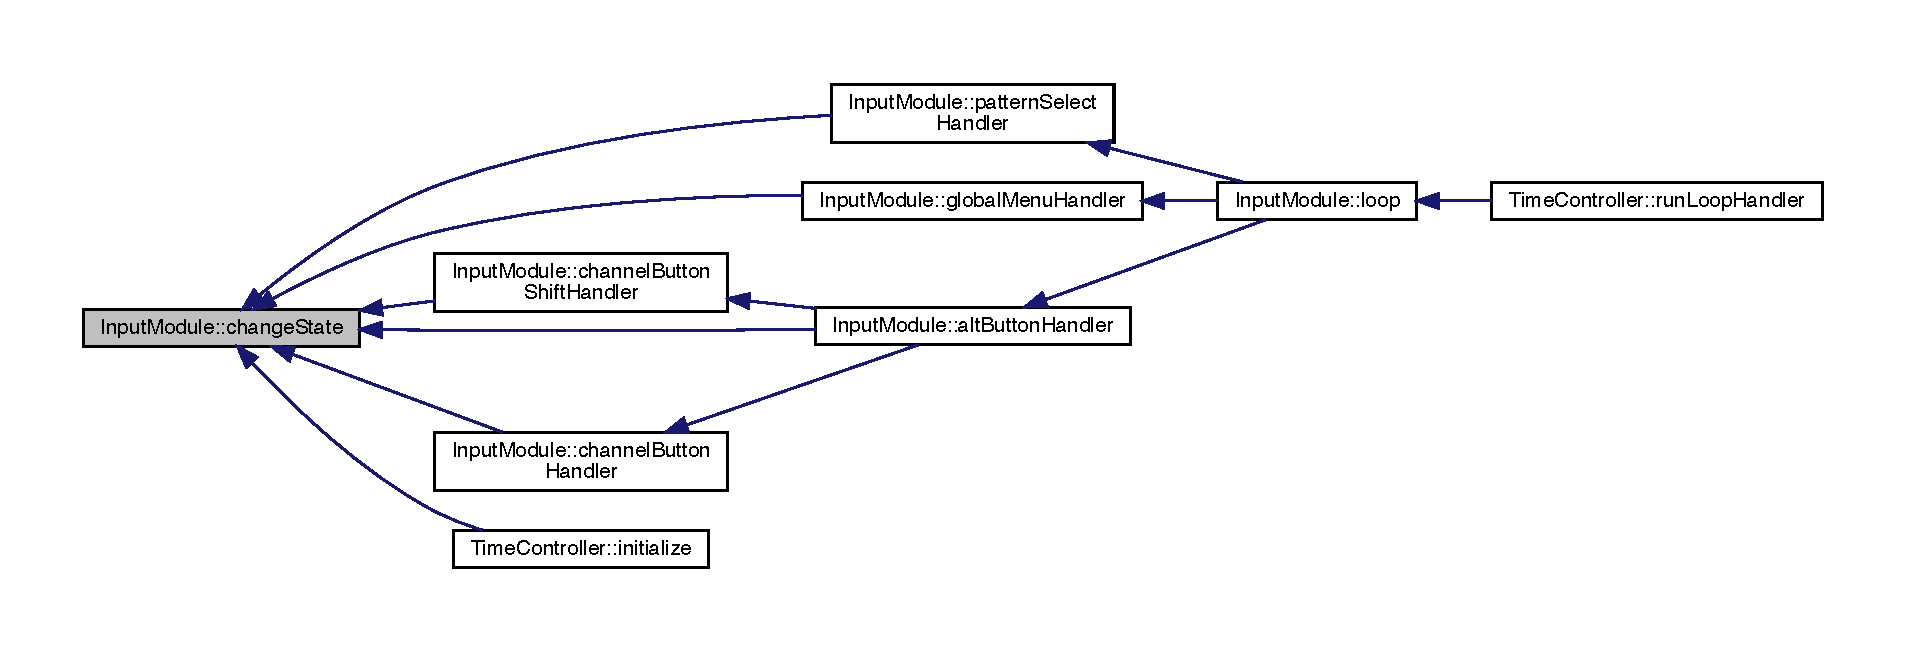
\includegraphics[width=350pt]{class_input_module_ac6242c4331441ba020d2fca7bff7a401_icgraph}
\end{center}
\end{figure}
\mbox{\Hypertarget{class_input_module_a62ad05f2e4880aeae014d99ecfcd494d}\label{class_input_module_a62ad05f2e4880aeae014d99ecfcd494d}} 
\index{Input\+Module@{Input\+Module}!channel\+Button\+Handler@{channel\+Button\+Handler}}
\index{channel\+Button\+Handler@{channel\+Button\+Handler}!Input\+Module@{Input\+Module}}
\subsubsection{\texorpdfstring{channel\+Button\+Handler()}{channelButtonHandler()}}
{\footnotesize\ttfamily void Input\+Module\+::channel\+Button\+Handler (\begin{DoxyParamCaption}\item[{uint8\+\_\+t}]{channel }\end{DoxyParamCaption})}

Here is the call graph for this function\+:
\nopagebreak
\begin{figure}[H]
\begin{center}
\leavevmode
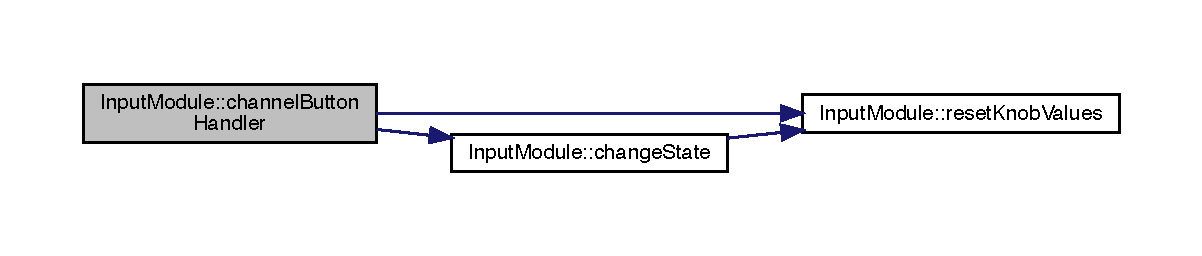
\includegraphics[width=350pt]{class_input_module_a62ad05f2e4880aeae014d99ecfcd494d_cgraph}
\end{center}
\end{figure}
Here is the caller graph for this function\+:
\nopagebreak
\begin{figure}[H]
\begin{center}
\leavevmode
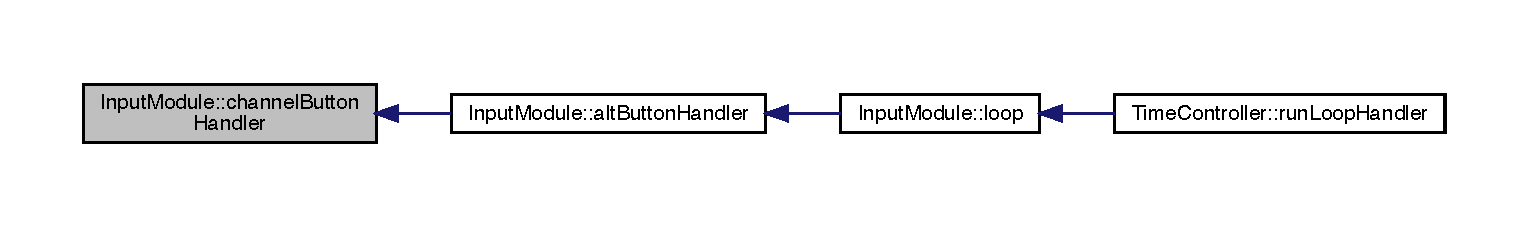
\includegraphics[width=350pt]{class_input_module_a62ad05f2e4880aeae014d99ecfcd494d_icgraph}
\end{center}
\end{figure}
\mbox{\Hypertarget{class_input_module_a2e678e1a6f2d7b9f91a6e6f1e3125e89}\label{class_input_module_a2e678e1a6f2d7b9f91a6e6f1e3125e89}} 
\index{Input\+Module@{Input\+Module}!channel\+Button\+Shift\+Handler@{channel\+Button\+Shift\+Handler}}
\index{channel\+Button\+Shift\+Handler@{channel\+Button\+Shift\+Handler}!Input\+Module@{Input\+Module}}
\subsubsection{\texorpdfstring{channel\+Button\+Shift\+Handler()}{channelButtonShiftHandler()}}
{\footnotesize\ttfamily void Input\+Module\+::channel\+Button\+Shift\+Handler (\begin{DoxyParamCaption}\item[{uint8\+\_\+t}]{channel }\end{DoxyParamCaption})}

Here is the call graph for this function\+:
\nopagebreak
\begin{figure}[H]
\begin{center}
\leavevmode
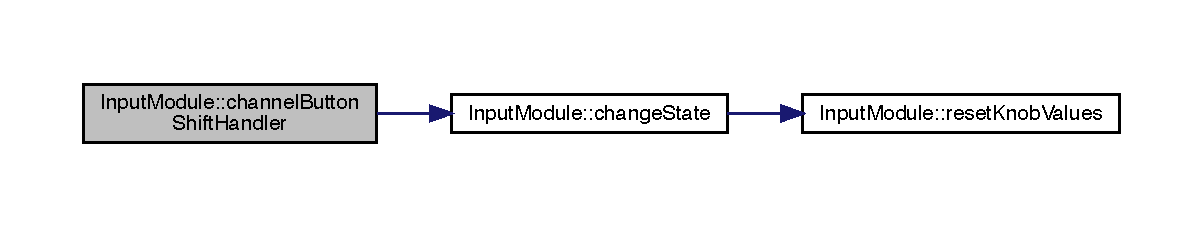
\includegraphics[width=350pt]{class_input_module_a2e678e1a6f2d7b9f91a6e6f1e3125e89_cgraph}
\end{center}
\end{figure}
Here is the caller graph for this function\+:
\nopagebreak
\begin{figure}[H]
\begin{center}
\leavevmode
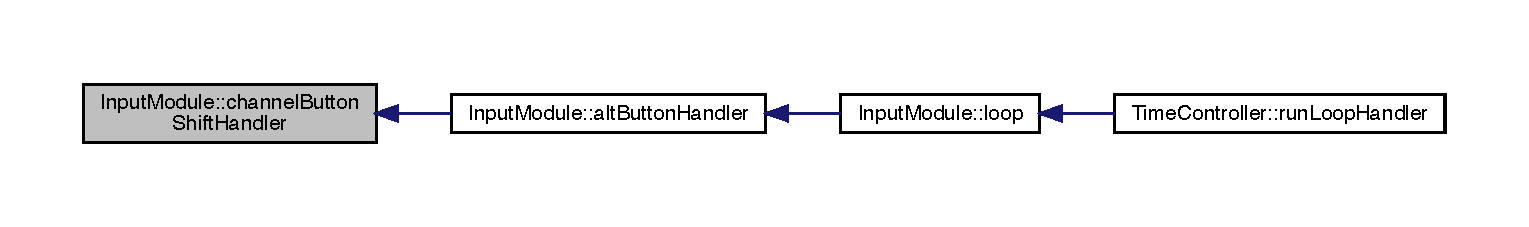
\includegraphics[width=350pt]{class_input_module_a2e678e1a6f2d7b9f91a6e6f1e3125e89_icgraph}
\end{center}
\end{figure}
\mbox{\Hypertarget{class_input_module_a0ff214fef897f5dd0bd0384673742996}\label{class_input_module_a0ff214fef897f5dd0bd0384673742996}} 
\index{Input\+Module@{Input\+Module}!channel\+Envelope\+Mode\+Input\+Handler@{channel\+Envelope\+Mode\+Input\+Handler}}
\index{channel\+Envelope\+Mode\+Input\+Handler@{channel\+Envelope\+Mode\+Input\+Handler}!Input\+Module@{Input\+Module}}
\subsubsection{\texorpdfstring{channel\+Envelope\+Mode\+Input\+Handler()}{channelEnvelopeModeInputHandler()}}
{\footnotesize\ttfamily void Input\+Module\+::channel\+Envelope\+Mode\+Input\+Handler (\begin{DoxyParamCaption}{ }\end{DoxyParamCaption})}

Here is the caller graph for this function\+:
\nopagebreak
\begin{figure}[H]
\begin{center}
\leavevmode
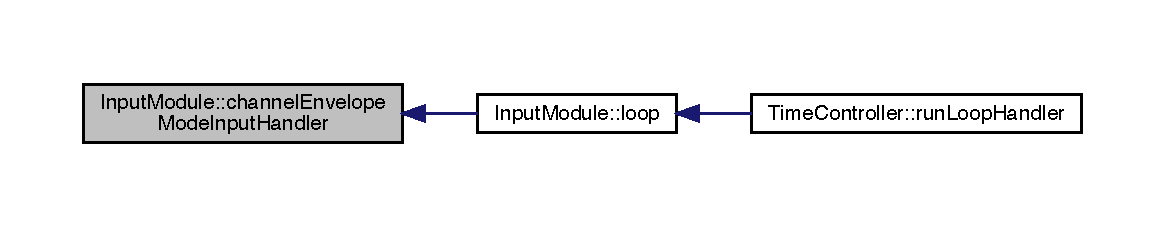
\includegraphics[width=350pt]{class_input_module_a0ff214fef897f5dd0bd0384673742996_icgraph}
\end{center}
\end{figure}
\mbox{\Hypertarget{class_input_module_af8193a3e5f84adb8a139d624742b8c6a}\label{class_input_module_af8193a3e5f84adb8a139d624742b8c6a}} 
\index{Input\+Module@{Input\+Module}!channel\+Pitch\+Mode\+Input\+Handler@{channel\+Pitch\+Mode\+Input\+Handler}}
\index{channel\+Pitch\+Mode\+Input\+Handler@{channel\+Pitch\+Mode\+Input\+Handler}!Input\+Module@{Input\+Module}}
\subsubsection{\texorpdfstring{channel\+Pitch\+Mode\+Input\+Handler()}{channelPitchModeInputHandler()}}
{\footnotesize\ttfamily void Input\+Module\+::channel\+Pitch\+Mode\+Input\+Handler (\begin{DoxyParamCaption}{ }\end{DoxyParamCaption})}

Here is the call graph for this function\+:
\nopagebreak
\begin{figure}[H]
\begin{center}
\leavevmode
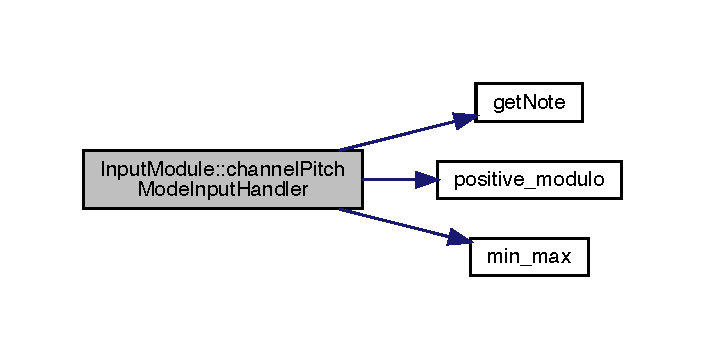
\includegraphics[width=338pt]{class_input_module_af8193a3e5f84adb8a139d624742b8c6a_cgraph}
\end{center}
\end{figure}
Here is the caller graph for this function\+:
\nopagebreak
\begin{figure}[H]
\begin{center}
\leavevmode
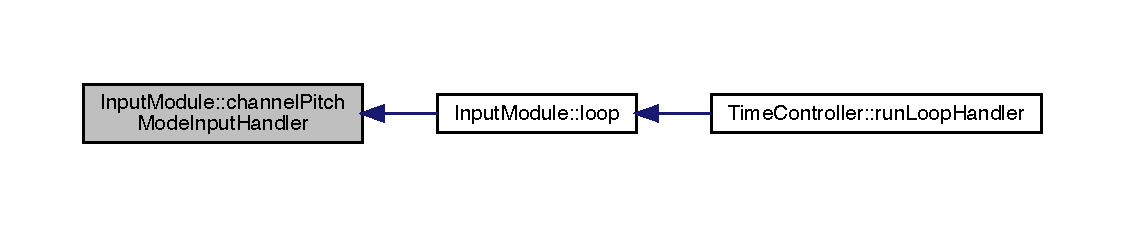
\includegraphics[width=350pt]{class_input_module_af8193a3e5f84adb8a139d624742b8c6a_icgraph}
\end{center}
\end{figure}
\mbox{\Hypertarget{class_input_module_ae5323fd937a03aff47a5696c67ca87d2}\label{class_input_module_ae5323fd937a03aff47a5696c67ca87d2}} 
\index{Input\+Module@{Input\+Module}!channel\+Step\+Mode\+Input\+Handler@{channel\+Step\+Mode\+Input\+Handler}}
\index{channel\+Step\+Mode\+Input\+Handler@{channel\+Step\+Mode\+Input\+Handler}!Input\+Module@{Input\+Module}}
\subsubsection{\texorpdfstring{channel\+Step\+Mode\+Input\+Handler()}{channelStepModeInputHandler()}}
{\footnotesize\ttfamily void Input\+Module\+::channel\+Step\+Mode\+Input\+Handler (\begin{DoxyParamCaption}{ }\end{DoxyParamCaption})}

Here is the caller graph for this function\+:
\nopagebreak
\begin{figure}[H]
\begin{center}
\leavevmode
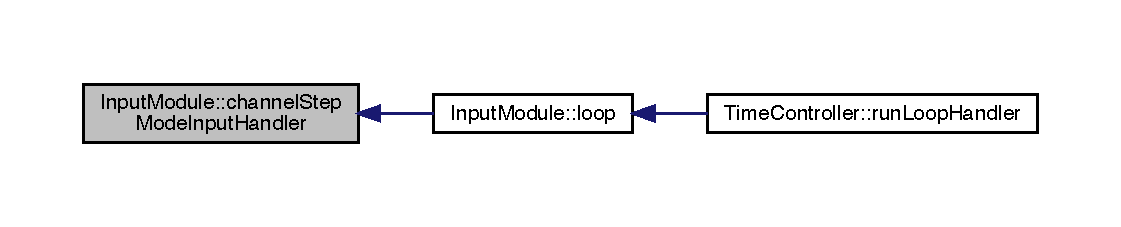
\includegraphics[width=350pt]{class_input_module_ae5323fd937a03aff47a5696c67ca87d2_icgraph}
\end{center}
\end{figure}
\mbox{\Hypertarget{class_input_module_a30c140bcc298b2c7c382ef290e77071f}\label{class_input_module_a30c140bcc298b2c7c382ef290e77071f}} 
\index{Input\+Module@{Input\+Module}!channel\+Velocity\+Mode\+Input\+Handler@{channel\+Velocity\+Mode\+Input\+Handler}}
\index{channel\+Velocity\+Mode\+Input\+Handler@{channel\+Velocity\+Mode\+Input\+Handler}!Input\+Module@{Input\+Module}}
\subsubsection{\texorpdfstring{channel\+Velocity\+Mode\+Input\+Handler()}{channelVelocityModeInputHandler()}}
{\footnotesize\ttfamily void Input\+Module\+::channel\+Velocity\+Mode\+Input\+Handler (\begin{DoxyParamCaption}{ }\end{DoxyParamCaption})}

Here is the call graph for this function\+:
\nopagebreak
\begin{figure}[H]
\begin{center}
\leavevmode
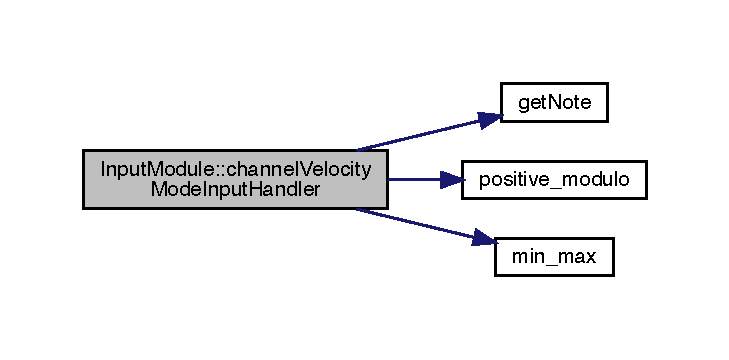
\includegraphics[width=350pt]{class_input_module_a30c140bcc298b2c7c382ef290e77071f_cgraph}
\end{center}
\end{figure}
Here is the caller graph for this function\+:
\nopagebreak
\begin{figure}[H]
\begin{center}
\leavevmode
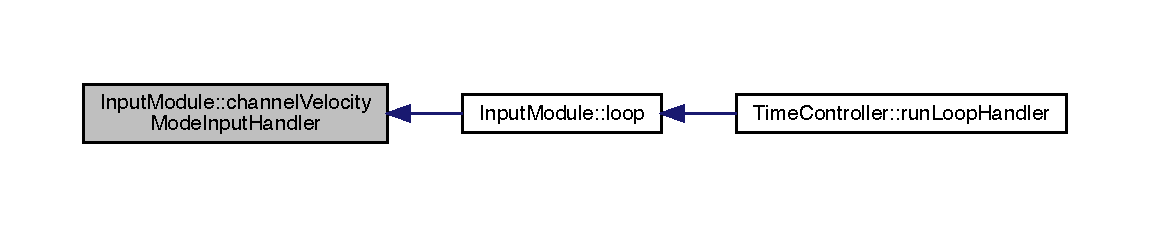
\includegraphics[width=350pt]{class_input_module_a30c140bcc298b2c7c382ef290e77071f_icgraph}
\end{center}
\end{figure}
\mbox{\Hypertarget{class_input_module_a341016de304d4ac105a9f5c98a76a853}\label{class_input_module_a341016de304d4ac105a9f5c98a76a853}} 
\index{Input\+Module@{Input\+Module}!debug\+Screen\+Input\+Handler@{debug\+Screen\+Input\+Handler}}
\index{debug\+Screen\+Input\+Handler@{debug\+Screen\+Input\+Handler}!Input\+Module@{Input\+Module}}
\subsubsection{\texorpdfstring{debug\+Screen\+Input\+Handler()}{debugScreenInputHandler()}}
{\footnotesize\ttfamily void Input\+Module\+::debug\+Screen\+Input\+Handler (\begin{DoxyParamCaption}{ }\end{DoxyParamCaption})}

Here is the caller graph for this function\+:
\nopagebreak
\begin{figure}[H]
\begin{center}
\leavevmode
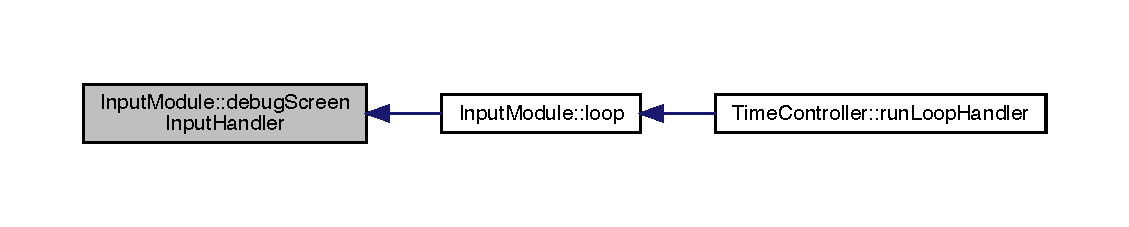
\includegraphics[width=350pt]{class_input_module_a341016de304d4ac105a9f5c98a76a853_icgraph}
\end{center}
\end{figure}
\mbox{\Hypertarget{class_input_module_a9844fa2022c8e526c431cd084556ffe0}\label{class_input_module_a9844fa2022c8e526c431cd084556ffe0}} 
\index{Input\+Module@{Input\+Module}!global\+Menu\+Handler@{global\+Menu\+Handler}}
\index{global\+Menu\+Handler@{global\+Menu\+Handler}!Input\+Module@{Input\+Module}}
\subsubsection{\texorpdfstring{global\+Menu\+Handler()}{globalMenuHandler()}}
{\footnotesize\ttfamily void Input\+Module\+::global\+Menu\+Handler (\begin{DoxyParamCaption}{ }\end{DoxyParamCaption})}

Here is the call graph for this function\+:
\nopagebreak
\begin{figure}[H]
\begin{center}
\leavevmode
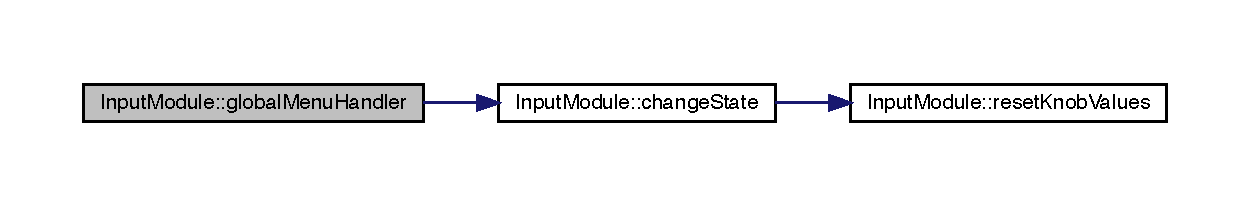
\includegraphics[width=350pt]{class_input_module_a9844fa2022c8e526c431cd084556ffe0_cgraph}
\end{center}
\end{figure}
Here is the caller graph for this function\+:
\nopagebreak
\begin{figure}[H]
\begin{center}
\leavevmode
\includegraphics[width=350pt]{class_input_module_a9844fa2022c8e526c431cd084556ffe0_icgraph}
\end{center}
\end{figure}
\mbox{\Hypertarget{class_input_module_a789c6f0da21e6b5b89c7c6991f4ee745}\label{class_input_module_a789c6f0da21e6b5b89c7c6991f4ee745}} 
\index{Input\+Module@{Input\+Module}!initialize@{initialize}}
\index{initialize@{initialize}!Input\+Module@{Input\+Module}}
\subsubsection{\texorpdfstring{initialize()}{initialize()}}
{\footnotesize\ttfamily void Input\+Module\+::initialize (\begin{DoxyParamCaption}\item[{\hyperlink{class_output_controller}{Output\+Controller} $\ast$}]{output\+Control,  }\item[{Zetaohm\+\_\+\+M\+A\+X7301 $\ast$}]{midplane\+G\+P\+IO,  }\item[{Zetaohm\+\_\+\+M\+A\+X7301 $\ast$}]{backplane\+G\+P\+IO,  }\item[{Flash\+Memory $\ast$}]{save\+File,  }\item[{Sequencer $\ast$}]{sequence\+Array,  }\item[{\hyperlink{class_master_clock}{Master\+Clock} $\ast$}]{clock\+Master }\end{DoxyParamCaption})}

Here is the caller graph for this function\+:
\nopagebreak
\begin{figure}[H]
\begin{center}
\leavevmode
\includegraphics[width=350pt]{class_input_module_a789c6f0da21e6b5b89c7c6991f4ee745_icgraph}
\end{center}
\end{figure}
\mbox{\Hypertarget{class_input_module_ad481ab7241ffe3a168e063a5afd6d892}\label{class_input_module_ad481ab7241ffe3a168e063a5afd6d892}} 
\index{Input\+Module@{Input\+Module}!loop@{loop}}
\index{loop@{loop}!Input\+Module@{Input\+Module}}
\subsubsection{\texorpdfstring{loop()}{loop()}}
{\footnotesize\ttfamily void Input\+Module\+::loop (\begin{DoxyParamCaption}\item[{uint16\+\_\+t}]{frequency }\end{DoxyParamCaption})}

Here is the call graph for this function\+:
\nopagebreak
\begin{figure}[H]
\begin{center}
\leavevmode
\includegraphics[width=350pt]{class_input_module_ad481ab7241ffe3a168e063a5afd6d892_cgraph}
\end{center}
\end{figure}
Here is the caller graph for this function\+:
\nopagebreak
\begin{figure}[H]
\begin{center}
\leavevmode
\includegraphics[width=350pt]{class_input_module_ad481ab7241ffe3a168e063a5afd6d892_icgraph}
\end{center}
\end{figure}
\mbox{\Hypertarget{class_input_module_a92fa77f3667cbfdce6c2fbdc14854811}\label{class_input_module_a92fa77f3667cbfdce6c2fbdc14854811}} 
\index{Input\+Module@{Input\+Module}!pattern\+Select\+Handler@{pattern\+Select\+Handler}}
\index{pattern\+Select\+Handler@{pattern\+Select\+Handler}!Input\+Module@{Input\+Module}}
\subsubsection{\texorpdfstring{pattern\+Select\+Handler()}{patternSelectHandler()}}
{\footnotesize\ttfamily void Input\+Module\+::pattern\+Select\+Handler (\begin{DoxyParamCaption}{ }\end{DoxyParamCaption})}

Here is the call graph for this function\+:
\nopagebreak
\begin{figure}[H]
\begin{center}
\leavevmode
\includegraphics[width=350pt]{class_input_module_a92fa77f3667cbfdce6c2fbdc14854811_cgraph}
\end{center}
\end{figure}
Here is the caller graph for this function\+:
\nopagebreak
\begin{figure}[H]
\begin{center}
\leavevmode
\includegraphics[width=350pt]{class_input_module_a92fa77f3667cbfdce6c2fbdc14854811_icgraph}
\end{center}
\end{figure}
\mbox{\Hypertarget{class_input_module_a1bbac8d8d543c1adfdaa955f251db63a}\label{class_input_module_a1bbac8d8d543c1adfdaa955f251db63a}} 
\index{Input\+Module@{Input\+Module}!reset\+Knob\+Values@{reset\+Knob\+Values}}
\index{reset\+Knob\+Values@{reset\+Knob\+Values}!Input\+Module@{Input\+Module}}
\subsubsection{\texorpdfstring{reset\+Knob\+Values()}{resetKnobValues()}}
{\footnotesize\ttfamily void Input\+Module\+::reset\+Knob\+Values (\begin{DoxyParamCaption}{ }\end{DoxyParamCaption})}

Here is the caller graph for this function\+:
\nopagebreak
\begin{figure}[H]
\begin{center}
\leavevmode
\includegraphics[width=350pt]{class_input_module_a1bbac8d8d543c1adfdaa955f251db63a_icgraph}
\end{center}
\end{figure}
\mbox{\Hypertarget{class_input_module_a6b0c9027e4088393722d00d162e4ecd9}\label{class_input_module_a6b0c9027e4088393722d00d162e4ecd9}} 
\index{Input\+Module@{Input\+Module}!sequence\+Menu\+Handler@{sequence\+Menu\+Handler}}
\index{sequence\+Menu\+Handler@{sequence\+Menu\+Handler}!Input\+Module@{Input\+Module}}
\subsubsection{\texorpdfstring{sequence\+Menu\+Handler()}{sequenceMenuHandler()}}
{\footnotesize\ttfamily void Input\+Module\+::sequence\+Menu\+Handler (\begin{DoxyParamCaption}{ }\end{DoxyParamCaption})}

Here is the call graph for this function\+:
\nopagebreak
\begin{figure}[H]
\begin{center}
\leavevmode
\includegraphics[width=349pt]{class_input_module_a6b0c9027e4088393722d00d162e4ecd9_cgraph}
\end{center}
\end{figure}
Here is the caller graph for this function\+:
\nopagebreak
\begin{figure}[H]
\begin{center}
\leavevmode
\includegraphics[width=350pt]{class_input_module_a6b0c9027e4088393722d00d162e4ecd9_icgraph}
\end{center}
\end{figure}
\mbox{\Hypertarget{class_input_module_ada290dc92f0ad59826c47781ea2209c0}\label{class_input_module_ada290dc92f0ad59826c47781ea2209c0}} 
\index{Input\+Module@{Input\+Module}!step\+Mode\+Matrix\+Handler@{step\+Mode\+Matrix\+Handler}}
\index{step\+Mode\+Matrix\+Handler@{step\+Mode\+Matrix\+Handler}!Input\+Module@{Input\+Module}}
\subsubsection{\texorpdfstring{step\+Mode\+Matrix\+Handler()}{stepModeMatrixHandler()}}
{\footnotesize\ttfamily void Input\+Module\+::step\+Mode\+Matrix\+Handler (\begin{DoxyParamCaption}{ }\end{DoxyParamCaption})}

\mbox{\Hypertarget{class_input_module_a2e71a13d6f8365f5753fae8f4542769c}\label{class_input_module_a2e71a13d6f8365f5753fae8f4542769c}} 
\index{Input\+Module@{Input\+Module}!tempo\+Menu\+Handler@{tempo\+Menu\+Handler}}
\index{tempo\+Menu\+Handler@{tempo\+Menu\+Handler}!Input\+Module@{Input\+Module}}
\subsubsection{\texorpdfstring{tempo\+Menu\+Handler()}{tempoMenuHandler()}}
{\footnotesize\ttfamily void Input\+Module\+::tempo\+Menu\+Handler (\begin{DoxyParamCaption}{ }\end{DoxyParamCaption})}

Here is the call graph for this function\+:
\nopagebreak
\begin{figure}[H]
\begin{center}
\leavevmode
\includegraphics[width=350pt]{class_input_module_a2e71a13d6f8365f5753fae8f4542769c_cgraph}
\end{center}
\end{figure}
Here is the caller graph for this function\+:
\nopagebreak
\begin{figure}[H]
\begin{center}
\leavevmode
\includegraphics[width=350pt]{class_input_module_a2e71a13d6f8365f5753fae8f4542769c_icgraph}
\end{center}
\end{figure}
\mbox{\Hypertarget{class_input_module_ab5048e031568fa6879b6618e4478cc97}\label{class_input_module_ab5048e031568fa6879b6618e4478cc97}} 
\index{Input\+Module@{Input\+Module}!timing\+Menu\+Input\+Handler@{timing\+Menu\+Input\+Handler}}
\index{timing\+Menu\+Input\+Handler@{timing\+Menu\+Input\+Handler}!Input\+Module@{Input\+Module}}
\subsubsection{\texorpdfstring{timing\+Menu\+Input\+Handler()}{timingMenuInputHandler()}}
{\footnotesize\ttfamily void Input\+Module\+::timing\+Menu\+Input\+Handler (\begin{DoxyParamCaption}{ }\end{DoxyParamCaption})}

Here is the caller graph for this function\+:
\nopagebreak
\begin{figure}[H]
\begin{center}
\leavevmode
\includegraphics[width=350pt]{class_input_module_ab5048e031568fa6879b6618e4478cc97_icgraph}
\end{center}
\end{figure}


\subsection{Member Data Documentation}
\mbox{\Hypertarget{class_input_module_a433abde922dee6f2abed80710f49a294}\label{class_input_module_a433abde922dee6f2abed80710f49a294}} 
\index{Input\+Module@{Input\+Module}!backplane\+G\+P\+IO@{backplane\+G\+P\+IO}}
\index{backplane\+G\+P\+IO@{backplane\+G\+P\+IO}!Input\+Module@{Input\+Module}}
\subsubsection{\texorpdfstring{backplane\+G\+P\+IO}{backplaneGPIO}}
{\footnotesize\ttfamily Zetaohm\+\_\+\+M\+A\+X7301$\ast$ Input\+Module\+::backplane\+G\+P\+IO}

\mbox{\Hypertarget{class_input_module_aff739621e5d47367263551f43d98b94b}\label{class_input_module_aff739621e5d47367263551f43d98b94b}} 
\index{Input\+Module@{Input\+Module}!clock\+Master@{clock\+Master}}
\index{clock\+Master@{clock\+Master}!Input\+Module@{Input\+Module}}
\subsubsection{\texorpdfstring{clock\+Master}{clockMaster}}
{\footnotesize\ttfamily \hyperlink{class_master_clock}{Master\+Clock}$\ast$ Input\+Module\+::clock\+Master}

\mbox{\Hypertarget{class_input_module_a56b62ba8836c0fb6ed93ca126bf9a02d}\label{class_input_module_a56b62ba8836c0fb6ed93ca126bf9a02d}} 
\index{Input\+Module@{Input\+Module}!encoder\+Button\+Time@{encoder\+Button\+Time}}
\index{encoder\+Button\+Time@{encoder\+Button\+Time}!Input\+Module@{Input\+Module}}
\subsubsection{\texorpdfstring{encoder\+Button\+Time}{encoderButtonTime}}
{\footnotesize\ttfamily unsigned long Input\+Module\+::encoder\+Button\+Time}

\mbox{\Hypertarget{class_input_module_a8479fea0b1f501250aa5026844d6a1a9}\label{class_input_module_a8479fea0b1f501250aa5026844d6a1a9}} 
\index{Input\+Module@{Input\+Module}!encoder\+Loop\+Time@{encoder\+Loop\+Time}}
\index{encoder\+Loop\+Time@{encoder\+Loop\+Time}!Input\+Module@{Input\+Module}}
\subsubsection{\texorpdfstring{encoder\+Loop\+Time}{encoderLoopTime}}
{\footnotesize\ttfamily unsigned long Input\+Module\+::encoder\+Loop\+Time}

\mbox{\Hypertarget{class_input_module_ae0efc931ea904dda2e5b29f8c20181eb}\label{class_input_module_ae0efc931ea904dda2e5b29f8c20181eb}} 
\index{Input\+Module@{Input\+Module}!input\+Timer@{input\+Timer}}
\index{input\+Timer@{input\+Timer}!Input\+Module@{Input\+Module}}
\subsubsection{\texorpdfstring{input\+Timer}{inputTimer}}
{\footnotesize\ttfamily elapsed\+Micros Input\+Module\+::input\+Timer\hspace{0.3cm}{\ttfamily [private]}}

\mbox{\Hypertarget{class_input_module_af11a3cf014306369d13bc79c3f5e1bcb}\label{class_input_module_af11a3cf014306369d13bc79c3f5e1bcb}} 
\index{Input\+Module@{Input\+Module}!inst\+Buffer@{inst\+Buffer}}
\index{inst\+Buffer@{inst\+Buffer}!Input\+Module@{Input\+Module}}
\subsubsection{\texorpdfstring{inst\+Buffer}{instBuffer}}
{\footnotesize\ttfamily int8\+\_\+t Input\+Module\+::inst\+Buffer}

\mbox{\Hypertarget{class_input_module_a70e9413a995052805e5c1e6962e1ec46}\label{class_input_module_a70e9413a995052805e5c1e6962e1ec46}} 
\index{Input\+Module@{Input\+Module}!knob@{knob}}
\index{knob@{knob}!Input\+Module@{Input\+Module}}
\subsubsection{\texorpdfstring{knob}{knob}}
{\footnotesize\ttfamily Encoder Input\+Module\+::knob}

\mbox{\Hypertarget{class_input_module_a6015af9178f42735dd65a308fd132cea}\label{class_input_module_a6015af9178f42735dd65a308fd132cea}} 
\index{Input\+Module@{Input\+Module}!knob\+Buffer@{knob\+Buffer}}
\index{knob\+Buffer@{knob\+Buffer}!Input\+Module@{Input\+Module}}
\subsubsection{\texorpdfstring{knob\+Buffer}{knobBuffer}}
{\footnotesize\ttfamily int8\+\_\+t Input\+Module\+::knob\+Buffer}

\mbox{\Hypertarget{class_input_module_aa71dde7943b36a879ea305285c042e09}\label{class_input_module_aa71dde7943b36a879ea305285c042e09}} 
\index{Input\+Module@{Input\+Module}!knob\+Change@{knob\+Change}}
\index{knob\+Change@{knob\+Change}!Input\+Module@{Input\+Module}}
\subsubsection{\texorpdfstring{knob\+Change}{knobChange}}
{\footnotesize\ttfamily int8\+\_\+t Input\+Module\+::knob\+Change}

\mbox{\Hypertarget{class_input_module_ad66cbf5057aa15d9428ddb0a6936543a}\label{class_input_module_ad66cbf5057aa15d9428ddb0a6936543a}} 
\index{Input\+Module@{Input\+Module}!knob\+Previous@{knob\+Previous}}
\index{knob\+Previous@{knob\+Previous}!Input\+Module@{Input\+Module}}
\subsubsection{\texorpdfstring{knob\+Previous}{knobPrevious}}
{\footnotesize\ttfamily int8\+\_\+t Input\+Module\+::knob\+Previous}

\mbox{\Hypertarget{class_input_module_a0d7bca8e1d85982108bc2b1c8a9a41fd}\label{class_input_module_a0d7bca8e1d85982108bc2b1c8a9a41fd}} 
\index{Input\+Module@{Input\+Module}!knob\+Read@{knob\+Read}}
\index{knob\+Read@{knob\+Read}!Input\+Module@{Input\+Module}}
\subsubsection{\texorpdfstring{knob\+Read}{knobRead}}
{\footnotesize\ttfamily int8\+\_\+t Input\+Module\+::knob\+Read}

\mbox{\Hypertarget{class_input_module_ae4cc83ddf8ca352a05aef5d737e57bc1}\label{class_input_module_ae4cc83ddf8ca352a05aef5d737e57bc1}} 
\index{Input\+Module@{Input\+Module}!matrix\+Button\+Time@{matrix\+Button\+Time}}
\index{matrix\+Button\+Time@{matrix\+Button\+Time}!Input\+Module@{Input\+Module}}
\subsubsection{\texorpdfstring{matrix\+Button\+Time}{matrixButtonTime}}
{\footnotesize\ttfamily unsigned long Input\+Module\+::matrix\+Button\+Time}

\mbox{\Hypertarget{class_input_module_a0116c65513c2c09f3e09cdf55e55c4cd}\label{class_input_module_a0116c65513c2c09f3e09cdf55e55c4cd}} 
\index{Input\+Module@{Input\+Module}!menu\+Selector@{menu\+Selector}}
\index{menu\+Selector@{menu\+Selector}!Input\+Module@{Input\+Module}}
\subsubsection{\texorpdfstring{menu\+Selector}{menuSelector}}
{\footnotesize\ttfamily int8\+\_\+t Input\+Module\+::menu\+Selector}

\mbox{\Hypertarget{class_input_module_ad23720995ebd07355df926bb18e2260d}\label{class_input_module_ad23720995ebd07355df926bb18e2260d}} 
\index{Input\+Module@{Input\+Module}!midplane\+G\+P\+IO@{midplane\+G\+P\+IO}}
\index{midplane\+G\+P\+IO@{midplane\+G\+P\+IO}!Input\+Module@{Input\+Module}}
\subsubsection{\texorpdfstring{midplane\+G\+P\+IO}{midplaneGPIO}}
{\footnotesize\ttfamily Zetaohm\+\_\+\+M\+A\+X7301$\ast$ Input\+Module\+::midplane\+G\+P\+IO}

\mbox{\Hypertarget{class_input_module_ad1019ec5aac3175710630718e056e471}\label{class_input_module_ad1019ec5aac3175710630718e056e471}} 
\index{Input\+Module@{Input\+Module}!output\+Control@{output\+Control}}
\index{output\+Control@{output\+Control}!Input\+Module@{Input\+Module}}
\subsubsection{\texorpdfstring{output\+Control}{outputControl}}
{\footnotesize\ttfamily \hyperlink{class_output_controller}{Output\+Controller}$\ast$ Input\+Module\+::output\+Control}

\mbox{\Hypertarget{class_input_module_a0a4fbca5f978a217f47ed31082eaaecc}\label{class_input_module_a0a4fbca5f978a217f47ed31082eaaecc}} 
\index{Input\+Module@{Input\+Module}!save\+File@{save\+File}}
\index{save\+File@{save\+File}!Input\+Module@{Input\+Module}}
\subsubsection{\texorpdfstring{save\+File}{saveFile}}
{\footnotesize\ttfamily Flash\+Memory$\ast$ Input\+Module\+::save\+File\hspace{0.3cm}{\ttfamily [private]}}

\mbox{\Hypertarget{class_input_module_afdc54a8219ed5b5743201a00efd2cb72}\label{class_input_module_afdc54a8219ed5b5743201a00efd2cb72}} 
\index{Input\+Module@{Input\+Module}!sequence\+Array@{sequence\+Array}}
\index{sequence\+Array@{sequence\+Array}!Input\+Module@{Input\+Module}}
\subsubsection{\texorpdfstring{sequence\+Array}{sequenceArray}}
{\footnotesize\ttfamily Sequencer$\ast$ Input\+Module\+::sequence\+Array\hspace{0.3cm}{\ttfamily [private]}}

\mbox{\Hypertarget{class_input_module_ad8ba561dc4d0372e46a5b8a0e0eb82d9}\label{class_input_module_ad8ba561dc4d0372e46a5b8a0e0eb82d9}} 
\index{Input\+Module@{Input\+Module}!small\+Button\+Loop\+Time@{small\+Button\+Loop\+Time}}
\index{small\+Button\+Loop\+Time@{small\+Button\+Loop\+Time}!Input\+Module@{Input\+Module}}
\subsubsection{\texorpdfstring{small\+Button\+Loop\+Time}{smallButtonLoopTime}}
{\footnotesize\ttfamily unsigned long Input\+Module\+::small\+Button\+Loop\+Time}

\mbox{\Hypertarget{class_input_module_a0197f1734ab95dd812a7747c9c2374b5}\label{class_input_module_a0197f1734ab95dd812a7747c9c2374b5}} 
\index{Input\+Module@{Input\+Module}!step\+Mode\+Buffer@{step\+Mode\+Buffer}}
\index{step\+Mode\+Buffer@{step\+Mode\+Buffer}!Input\+Module@{Input\+Module}}
\subsubsection{\texorpdfstring{step\+Mode\+Buffer}{stepModeBuffer}}
{\footnotesize\ttfamily int16\+\_\+t Input\+Module\+::step\+Mode\+Buffer}



The documentation for this class was generated from the following files\+:\begin{DoxyCompactItemize}
\item 
src/\hyperlink{input_module_8h}{input\+Module.\+h}\item 
src/\hyperlink{input_module_8cpp}{input\+Module.\+cpp}\end{DoxyCompactItemize}

\hypertarget{class_l_e_d_array}{}\section{L\+E\+D\+Array Class Reference}
\label{class_l_e_d_array}\index{L\+E\+D\+Array@{L\+E\+D\+Array}}


{\ttfamily \#include $<$L\+E\+D\+Array.\+h$>$}

\subsection*{Public Member Functions}
\begin{DoxyCompactItemize}
\item 
\hyperlink{class_l_e_d_array_a38e049928e05c44035bf47ed888c319f}{L\+E\+D\+Array} ()
\item 
void \hyperlink{class_l_e_d_array_affcc24a132375e42e76f231da3744542}{initialize} (Sequencer $\ast$\hyperlink{class_l_e_d_array_a93c18ec03393f639c7e0a11a3324c922}{sequence\+Array})
\item 
void \hyperlink{class_l_e_d_array_a13f7dd3ae81862c31331199c732f8a3e}{loop} (uint16\+\_\+t \hyperlink{global_8h_acdfc8898c9e67fbcec81f3b04ae61bd9}{frequency})
\item 
void \hyperlink{class_l_e_d_array_aa9d1531481da8b4f236a8c187f986b0d}{fadeall} ()
\item 
void \hyperlink{class_l_e_d_array_af787dadd33b8c2049de93f8e91bc60ab}{rainbow\+Cycle} (uint8\+\_\+t wait)
\item 
uint32\+\_\+t \hyperlink{class_l_e_d_array_a783c6a0ef721d76b6b65aead2322e059}{wheel} (byte Wheel\+Pos)
\item 
void \hyperlink{class_l_e_d_array_a602c56fdb10d7bf66f8d681081a99b83}{channel\+Pitch\+Mode\+L\+E\+D\+Handler} ()
\item 
void \hyperlink{class_l_e_d_array_ab90f5a669b0faf8853070e12b99c4b3d}{channel\+Gate\+Mode\+L\+E\+D\+Handler} ()
\item 
void \hyperlink{class_l_e_d_array_a4fdfa734a42f2e2f577a0be7ce8953d5}{channel\+Envelope\+Mode\+L\+E\+D\+Handler} ()
\item 
void \hyperlink{class_l_e_d_array_a81dfe62b22624f9f29d57da0298043fc}{channel\+Step\+Mode\+L\+E\+D\+Handler} ()
\end{DoxyCompactItemize}
\subsection*{Private Attributes}
\begin{DoxyCompactItemize}
\item 
Sequencer $\ast$ \hyperlink{class_l_e_d_array_a93c18ec03393f639c7e0a11a3324c922}{sequence\+Array}
\item 
elapsed\+Micros \hyperlink{class_l_e_d_array_a72681582a31026c79a8021cead72d51e}{pixel\+Timer}
\item 
Adafruit\+\_\+\+Neo\+Pixel \hyperlink{class_l_e_d_array_ae781b0d4364e6789f618e9d73fe69198}{leds} = Adafruit\+\_\+\+Neo\+Pixel(\hyperlink{_l_e_d_array_8h_a4c4ae9a4146ce8d6a5debc90300d9abd}{N\+U\+M\+\_\+\+L\+E\+DS}, \hyperlink{_l_e_d_array_8h_adad67fe595ea440c8f8247ec2cddf070}{D\+A\+T\+A\+\_\+\+P\+IN}, N\+E\+O\+\_\+\+G\+R\+BW + N\+E\+O\+\_\+\+K\+H\+Z800)
\item 
uint8\+\_\+t \hyperlink{class_l_e_d_array_a9a675b5ebd4e5b0034ef944f204871fe}{led\+Mapping} \mbox{[}\hyperlink{_l_e_d_array_8h_a4c4ae9a4146ce8d6a5debc90300d9abd}{N\+U\+M\+\_\+\+L\+E\+DS}\mbox{]} = \{1,2,3,4,6,7,8,9,11,12,13,14,16,17,18,19,0,5,10,15\}
\item 
uint8\+\_\+t \hyperlink{class_l_e_d_array_add6bd6e431a7e4a8b7e33c96b0bf7578}{led\+Main\+Matrix} \mbox{[}16\mbox{]} = \{2,3,4,5,7,8,9,10,12,13,14,15,17,18,19,20\}
\item 
uint8\+\_\+t \hyperlink{class_l_e_d_array_a64d8cc06323de69ccad888f63a231c5f}{led\+Channel\+Buttons} \mbox{[}4\mbox{]} = \{1,6,11,16\}
\item 
uint8\+\_\+t \hyperlink{class_l_e_d_array_a22ca5391b4ad6c8b7b44e3aaf73c9429}{led\+Aux\+Buttons} \mbox{[}3\mbox{]} = \{0,21,22\}
\end{DoxyCompactItemize}


\subsection{Constructor \& Destructor Documentation}
\mbox{\Hypertarget{class_l_e_d_array_a38e049928e05c44035bf47ed888c319f}\label{class_l_e_d_array_a38e049928e05c44035bf47ed888c319f}} 
\index{L\+E\+D\+Array@{L\+E\+D\+Array}!L\+E\+D\+Array@{L\+E\+D\+Array}}
\index{L\+E\+D\+Array@{L\+E\+D\+Array}!L\+E\+D\+Array@{L\+E\+D\+Array}}
\subsubsection{\texorpdfstring{L\+E\+D\+Array()}{LEDArray()}}
{\footnotesize\ttfamily L\+E\+D\+Array\+::\+L\+E\+D\+Array (\begin{DoxyParamCaption}{ }\end{DoxyParamCaption})}



\subsection{Member Function Documentation}
\mbox{\Hypertarget{class_l_e_d_array_a4fdfa734a42f2e2f577a0be7ce8953d5}\label{class_l_e_d_array_a4fdfa734a42f2e2f577a0be7ce8953d5}} 
\index{L\+E\+D\+Array@{L\+E\+D\+Array}!channel\+Envelope\+Mode\+L\+E\+D\+Handler@{channel\+Envelope\+Mode\+L\+E\+D\+Handler}}
\index{channel\+Envelope\+Mode\+L\+E\+D\+Handler@{channel\+Envelope\+Mode\+L\+E\+D\+Handler}!L\+E\+D\+Array@{L\+E\+D\+Array}}
\subsubsection{\texorpdfstring{channel\+Envelope\+Mode\+L\+E\+D\+Handler()}{channelEnvelopeModeLEDHandler()}}
{\footnotesize\ttfamily void L\+E\+D\+Array\+::channel\+Envelope\+Mode\+L\+E\+D\+Handler (\begin{DoxyParamCaption}{ }\end{DoxyParamCaption})}

Here is the call graph for this function\+:
\nopagebreak
\begin{figure}[H]
\begin{center}
\leavevmode
\includegraphics[width=349pt]{class_l_e_d_array_a4fdfa734a42f2e2f577a0be7ce8953d5_cgraph}
\end{center}
\end{figure}
Here is the caller graph for this function\+:
\nopagebreak
\begin{figure}[H]
\begin{center}
\leavevmode
\includegraphics[width=350pt]{class_l_e_d_array_a4fdfa734a42f2e2f577a0be7ce8953d5_icgraph}
\end{center}
\end{figure}
\mbox{\Hypertarget{class_l_e_d_array_ab90f5a669b0faf8853070e12b99c4b3d}\label{class_l_e_d_array_ab90f5a669b0faf8853070e12b99c4b3d}} 
\index{L\+E\+D\+Array@{L\+E\+D\+Array}!channel\+Gate\+Mode\+L\+E\+D\+Handler@{channel\+Gate\+Mode\+L\+E\+D\+Handler}}
\index{channel\+Gate\+Mode\+L\+E\+D\+Handler@{channel\+Gate\+Mode\+L\+E\+D\+Handler}!L\+E\+D\+Array@{L\+E\+D\+Array}}
\subsubsection{\texorpdfstring{channel\+Gate\+Mode\+L\+E\+D\+Handler()}{channelGateModeLEDHandler()}}
{\footnotesize\ttfamily void L\+E\+D\+Array\+::channel\+Gate\+Mode\+L\+E\+D\+Handler (\begin{DoxyParamCaption}{ }\end{DoxyParamCaption})}

Here is the call graph for this function\+:
\nopagebreak
\begin{figure}[H]
\begin{center}
\leavevmode
\includegraphics[width=350pt]{class_l_e_d_array_ab90f5a669b0faf8853070e12b99c4b3d_cgraph}
\end{center}
\end{figure}
Here is the caller graph for this function\+:
\nopagebreak
\begin{figure}[H]
\begin{center}
\leavevmode
\includegraphics[width=350pt]{class_l_e_d_array_ab90f5a669b0faf8853070e12b99c4b3d_icgraph}
\end{center}
\end{figure}
\mbox{\Hypertarget{class_l_e_d_array_a602c56fdb10d7bf66f8d681081a99b83}\label{class_l_e_d_array_a602c56fdb10d7bf66f8d681081a99b83}} 
\index{L\+E\+D\+Array@{L\+E\+D\+Array}!channel\+Pitch\+Mode\+L\+E\+D\+Handler@{channel\+Pitch\+Mode\+L\+E\+D\+Handler}}
\index{channel\+Pitch\+Mode\+L\+E\+D\+Handler@{channel\+Pitch\+Mode\+L\+E\+D\+Handler}!L\+E\+D\+Array@{L\+E\+D\+Array}}
\subsubsection{\texorpdfstring{channel\+Pitch\+Mode\+L\+E\+D\+Handler()}{channelPitchModeLEDHandler()}}
{\footnotesize\ttfamily void L\+E\+D\+Array\+::channel\+Pitch\+Mode\+L\+E\+D\+Handler (\begin{DoxyParamCaption}{ }\end{DoxyParamCaption})}

Here is the call graph for this function\+:
\nopagebreak
\begin{figure}[H]
\begin{center}
\leavevmode
\includegraphics[width=350pt]{class_l_e_d_array_a602c56fdb10d7bf66f8d681081a99b83_cgraph}
\end{center}
\end{figure}
Here is the caller graph for this function\+:
\nopagebreak
\begin{figure}[H]
\begin{center}
\leavevmode
\includegraphics[width=350pt]{class_l_e_d_array_a602c56fdb10d7bf66f8d681081a99b83_icgraph}
\end{center}
\end{figure}
\mbox{\Hypertarget{class_l_e_d_array_a81dfe62b22624f9f29d57da0298043fc}\label{class_l_e_d_array_a81dfe62b22624f9f29d57da0298043fc}} 
\index{L\+E\+D\+Array@{L\+E\+D\+Array}!channel\+Step\+Mode\+L\+E\+D\+Handler@{channel\+Step\+Mode\+L\+E\+D\+Handler}}
\index{channel\+Step\+Mode\+L\+E\+D\+Handler@{channel\+Step\+Mode\+L\+E\+D\+Handler}!L\+E\+D\+Array@{L\+E\+D\+Array}}
\subsubsection{\texorpdfstring{channel\+Step\+Mode\+L\+E\+D\+Handler()}{channelStepModeLEDHandler()}}
{\footnotesize\ttfamily void L\+E\+D\+Array\+::channel\+Step\+Mode\+L\+E\+D\+Handler (\begin{DoxyParamCaption}{ }\end{DoxyParamCaption})}

Here is the call graph for this function\+:
\nopagebreak
\begin{figure}[H]
\begin{center}
\leavevmode
\includegraphics[width=350pt]{class_l_e_d_array_a81dfe62b22624f9f29d57da0298043fc_cgraph}
\end{center}
\end{figure}
Here is the caller graph for this function\+:
\nopagebreak
\begin{figure}[H]
\begin{center}
\leavevmode
\includegraphics[width=350pt]{class_l_e_d_array_a81dfe62b22624f9f29d57da0298043fc_icgraph}
\end{center}
\end{figure}
\mbox{\Hypertarget{class_l_e_d_array_aa9d1531481da8b4f236a8c187f986b0d}\label{class_l_e_d_array_aa9d1531481da8b4f236a8c187f986b0d}} 
\index{L\+E\+D\+Array@{L\+E\+D\+Array}!fadeall@{fadeall}}
\index{fadeall@{fadeall}!L\+E\+D\+Array@{L\+E\+D\+Array}}
\subsubsection{\texorpdfstring{fadeall()}{fadeall()}}
{\footnotesize\ttfamily void L\+E\+D\+Array\+::fadeall (\begin{DoxyParamCaption}{ }\end{DoxyParamCaption})}

\mbox{\Hypertarget{class_l_e_d_array_affcc24a132375e42e76f231da3744542}\label{class_l_e_d_array_affcc24a132375e42e76f231da3744542}} 
\index{L\+E\+D\+Array@{L\+E\+D\+Array}!initialize@{initialize}}
\index{initialize@{initialize}!L\+E\+D\+Array@{L\+E\+D\+Array}}
\subsubsection{\texorpdfstring{initialize()}{initialize()}}
{\footnotesize\ttfamily void L\+E\+D\+Array\+::initialize (\begin{DoxyParamCaption}\item[{Sequencer $\ast$}]{sequence\+Array }\end{DoxyParamCaption})}

Here is the call graph for this function\+:
\nopagebreak
\begin{figure}[H]
\begin{center}
\leavevmode
\includegraphics[width=350pt]{class_l_e_d_array_affcc24a132375e42e76f231da3744542_cgraph}
\end{center}
\end{figure}
Here is the caller graph for this function\+:
\nopagebreak
\begin{figure}[H]
\begin{center}
\leavevmode
\includegraphics[width=339pt]{class_l_e_d_array_affcc24a132375e42e76f231da3744542_icgraph}
\end{center}
\end{figure}
\mbox{\Hypertarget{class_l_e_d_array_a13f7dd3ae81862c31331199c732f8a3e}\label{class_l_e_d_array_a13f7dd3ae81862c31331199c732f8a3e}} 
\index{L\+E\+D\+Array@{L\+E\+D\+Array}!loop@{loop}}
\index{loop@{loop}!L\+E\+D\+Array@{L\+E\+D\+Array}}
\subsubsection{\texorpdfstring{loop()}{loop()}}
{\footnotesize\ttfamily void L\+E\+D\+Array\+::loop (\begin{DoxyParamCaption}\item[{uint16\+\_\+t}]{frequency }\end{DoxyParamCaption})}

Here is the call graph for this function\+:
\nopagebreak
\begin{figure}[H]
\begin{center}
\leavevmode
\includegraphics[width=350pt]{class_l_e_d_array_a13f7dd3ae81862c31331199c732f8a3e_cgraph}
\end{center}
\end{figure}
Here is the caller graph for this function\+:
\nopagebreak
\begin{figure}[H]
\begin{center}
\leavevmode
\includegraphics[width=350pt]{class_l_e_d_array_a13f7dd3ae81862c31331199c732f8a3e_icgraph}
\end{center}
\end{figure}
\mbox{\Hypertarget{class_l_e_d_array_af787dadd33b8c2049de93f8e91bc60ab}\label{class_l_e_d_array_af787dadd33b8c2049de93f8e91bc60ab}} 
\index{L\+E\+D\+Array@{L\+E\+D\+Array}!rainbow\+Cycle@{rainbow\+Cycle}}
\index{rainbow\+Cycle@{rainbow\+Cycle}!L\+E\+D\+Array@{L\+E\+D\+Array}}
\subsubsection{\texorpdfstring{rainbow\+Cycle()}{rainbowCycle()}}
{\footnotesize\ttfamily void L\+E\+D\+Array\+::rainbow\+Cycle (\begin{DoxyParamCaption}\item[{uint8\+\_\+t}]{wait }\end{DoxyParamCaption})}

Here is the call graph for this function\+:
\nopagebreak
\begin{figure}[H]
\begin{center}
\leavevmode
\includegraphics[width=332pt]{class_l_e_d_array_af787dadd33b8c2049de93f8e91bc60ab_cgraph}
\end{center}
\end{figure}
Here is the caller graph for this function\+:
\nopagebreak
\begin{figure}[H]
\begin{center}
\leavevmode
\includegraphics[width=350pt]{class_l_e_d_array_af787dadd33b8c2049de93f8e91bc60ab_icgraph}
\end{center}
\end{figure}
\mbox{\Hypertarget{class_l_e_d_array_a783c6a0ef721d76b6b65aead2322e059}\label{class_l_e_d_array_a783c6a0ef721d76b6b65aead2322e059}} 
\index{L\+E\+D\+Array@{L\+E\+D\+Array}!wheel@{wheel}}
\index{wheel@{wheel}!L\+E\+D\+Array@{L\+E\+D\+Array}}
\subsubsection{\texorpdfstring{wheel()}{wheel()}}
{\footnotesize\ttfamily uint32\+\_\+t L\+E\+D\+Array\+::wheel (\begin{DoxyParamCaption}\item[{byte}]{Wheel\+Pos }\end{DoxyParamCaption})}

Here is the caller graph for this function\+:
\nopagebreak
\begin{figure}[H]
\begin{center}
\leavevmode
\includegraphics[width=350pt]{class_l_e_d_array_a783c6a0ef721d76b6b65aead2322e059_icgraph}
\end{center}
\end{figure}


\subsection{Member Data Documentation}
\mbox{\Hypertarget{class_l_e_d_array_a22ca5391b4ad6c8b7b44e3aaf73c9429}\label{class_l_e_d_array_a22ca5391b4ad6c8b7b44e3aaf73c9429}} 
\index{L\+E\+D\+Array@{L\+E\+D\+Array}!led\+Aux\+Buttons@{led\+Aux\+Buttons}}
\index{led\+Aux\+Buttons@{led\+Aux\+Buttons}!L\+E\+D\+Array@{L\+E\+D\+Array}}
\subsubsection{\texorpdfstring{led\+Aux\+Buttons}{ledAuxButtons}}
{\footnotesize\ttfamily uint8\+\_\+t L\+E\+D\+Array\+::led\+Aux\+Buttons\mbox{[}3\mbox{]} = \{0,21,22\}\hspace{0.3cm}{\ttfamily [private]}}

\mbox{\Hypertarget{class_l_e_d_array_a64d8cc06323de69ccad888f63a231c5f}\label{class_l_e_d_array_a64d8cc06323de69ccad888f63a231c5f}} 
\index{L\+E\+D\+Array@{L\+E\+D\+Array}!led\+Channel\+Buttons@{led\+Channel\+Buttons}}
\index{led\+Channel\+Buttons@{led\+Channel\+Buttons}!L\+E\+D\+Array@{L\+E\+D\+Array}}
\subsubsection{\texorpdfstring{led\+Channel\+Buttons}{ledChannelButtons}}
{\footnotesize\ttfamily uint8\+\_\+t L\+E\+D\+Array\+::led\+Channel\+Buttons\mbox{[}4\mbox{]} = \{1,6,11,16\}\hspace{0.3cm}{\ttfamily [private]}}

\mbox{\Hypertarget{class_l_e_d_array_add6bd6e431a7e4a8b7e33c96b0bf7578}\label{class_l_e_d_array_add6bd6e431a7e4a8b7e33c96b0bf7578}} 
\index{L\+E\+D\+Array@{L\+E\+D\+Array}!led\+Main\+Matrix@{led\+Main\+Matrix}}
\index{led\+Main\+Matrix@{led\+Main\+Matrix}!L\+E\+D\+Array@{L\+E\+D\+Array}}
\subsubsection{\texorpdfstring{led\+Main\+Matrix}{ledMainMatrix}}
{\footnotesize\ttfamily uint8\+\_\+t L\+E\+D\+Array\+::led\+Main\+Matrix\mbox{[}16\mbox{]} = \{2,3,4,5,7,8,9,10,12,13,14,15,17,18,19,20\}\hspace{0.3cm}{\ttfamily [private]}}

\mbox{\Hypertarget{class_l_e_d_array_a9a675b5ebd4e5b0034ef944f204871fe}\label{class_l_e_d_array_a9a675b5ebd4e5b0034ef944f204871fe}} 
\index{L\+E\+D\+Array@{L\+E\+D\+Array}!led\+Mapping@{led\+Mapping}}
\index{led\+Mapping@{led\+Mapping}!L\+E\+D\+Array@{L\+E\+D\+Array}}
\subsubsection{\texorpdfstring{led\+Mapping}{ledMapping}}
{\footnotesize\ttfamily uint8\+\_\+t L\+E\+D\+Array\+::led\+Mapping\mbox{[}\hyperlink{_l_e_d_array_8h_a4c4ae9a4146ce8d6a5debc90300d9abd}{N\+U\+M\+\_\+\+L\+E\+DS}\mbox{]} = \{1,2,3,4,6,7,8,9,11,12,13,14,16,17,18,19,0,5,10,15\}\hspace{0.3cm}{\ttfamily [private]}}

\mbox{\Hypertarget{class_l_e_d_array_ae781b0d4364e6789f618e9d73fe69198}\label{class_l_e_d_array_ae781b0d4364e6789f618e9d73fe69198}} 
\index{L\+E\+D\+Array@{L\+E\+D\+Array}!leds@{leds}}
\index{leds@{leds}!L\+E\+D\+Array@{L\+E\+D\+Array}}
\subsubsection{\texorpdfstring{leds}{leds}}
{\footnotesize\ttfamily Adafruit\+\_\+\+Neo\+Pixel L\+E\+D\+Array\+::leds = Adafruit\+\_\+\+Neo\+Pixel(\hyperlink{_l_e_d_array_8h_a4c4ae9a4146ce8d6a5debc90300d9abd}{N\+U\+M\+\_\+\+L\+E\+DS}, \hyperlink{_l_e_d_array_8h_adad67fe595ea440c8f8247ec2cddf070}{D\+A\+T\+A\+\_\+\+P\+IN}, N\+E\+O\+\_\+\+G\+R\+BW + N\+E\+O\+\_\+\+K\+H\+Z800)\hspace{0.3cm}{\ttfamily [private]}}

\mbox{\Hypertarget{class_l_e_d_array_a72681582a31026c79a8021cead72d51e}\label{class_l_e_d_array_a72681582a31026c79a8021cead72d51e}} 
\index{L\+E\+D\+Array@{L\+E\+D\+Array}!pixel\+Timer@{pixel\+Timer}}
\index{pixel\+Timer@{pixel\+Timer}!L\+E\+D\+Array@{L\+E\+D\+Array}}
\subsubsection{\texorpdfstring{pixel\+Timer}{pixelTimer}}
{\footnotesize\ttfamily elapsed\+Micros L\+E\+D\+Array\+::pixel\+Timer\hspace{0.3cm}{\ttfamily [private]}}

\mbox{\Hypertarget{class_l_e_d_array_a93c18ec03393f639c7e0a11a3324c922}\label{class_l_e_d_array_a93c18ec03393f639c7e0a11a3324c922}} 
\index{L\+E\+D\+Array@{L\+E\+D\+Array}!sequence\+Array@{sequence\+Array}}
\index{sequence\+Array@{sequence\+Array}!L\+E\+D\+Array@{L\+E\+D\+Array}}
\subsubsection{\texorpdfstring{sequence\+Array}{sequenceArray}}
{\footnotesize\ttfamily Sequencer$\ast$ L\+E\+D\+Array\+::sequence\+Array\hspace{0.3cm}{\ttfamily [private]}}



The documentation for this class was generated from the following files\+:\begin{DoxyCompactItemize}
\item 
src/\hyperlink{_l_e_d_array_8h}{L\+E\+D\+Array.\+h}\item 
src/\hyperlink{_l_e_d_array_8cpp}{L\+E\+D\+Array.\+cpp}\end{DoxyCompactItemize}

\hypertarget{class_master_clock}{}\section{Master\+Clock Class Reference}
\label{class_master_clock}\index{Master\+Clock@{Master\+Clock}}


{\ttfamily \#include $<$master\+Clock.\+h$>$}



Collaboration diagram for Master\+Clock\+:
\nopagebreak
\begin{figure}[H]
\begin{center}
\leavevmode
\includegraphics[width=256pt]{class_master_clock__coll__graph}
\end{center}
\end{figure}
\subsection*{Public Member Functions}
\begin{DoxyCompactItemize}
\item 
void \hyperlink{class_master_clock_aa7106b58216e1bc65dc88cdbba1d0514}{initialize} (\hyperlink{class_output_controller}{Output\+Controller} $\ast$\hyperlink{class_master_clock_a6ec5b571edf2361d6c02834dec70fc09}{output\+Control}, Sequencer $\ast$\hyperlink{class_master_clock_a5e1a8b89151a6f5698e0ee3a0923e7bb}{sequence\+Array}, midi\+::\+Midi\+Interface$<$ Hardware\+Serial $>$ $\ast$\hyperlink{class_master_clock_a4c93dc002c3c69bd93a4b694a9ae0834}{serial\+Midi}, \hyperlink{class_midi_module}{Midi\+Module} $\ast$\hyperlink{class_master_clock_ac38ecfe6fdbbe0d43fb7b09d32dd4999}{midi\+Control})
\item 
void \hyperlink{class_master_clock_a81cfc025162075b165cd8ff93da5489a}{change\+Tempo} (uint32\+\_\+t new\+Tempo\+X100)
\item 
void \hyperlink{class_master_clock_a6d2a014da8caf9c4f39917ce4c09b83d}{master\+Clock\+Func} ()
\item 
void \hyperlink{class_master_clock_a96924e6693fee4ac2f9994583d0f33ba}{internal\+Clock\+Tick} ()
\item 
void \hyperlink{class_master_clock_a9c19932a580f5c5797fd31a58dc1a410}{midi\+Clock\+Tick} ()
\item 
void \hyperlink{class_master_clock_ab64882eca80c7e2de0b9e57020661df9}{external\+Clock\+Tick} (uint8\+\_\+t gate\+Num)
\item 
bool \hyperlink{class_master_clock_a16c1149bcc96dbea9d57063ad7a65d17}{gate\+Trigger} (uint8\+\_\+t gate\+Num)
\item 
void \hyperlink{class_master_clock_a94e8a4d26a0bb028a132d7582d602f01}{check\+Gate\+Clock} ()
\end{DoxyCompactItemize}
\subsection*{Public Attributes}
\begin{DoxyCompactItemize}
\item 
bool \hyperlink{class_master_clock_a5c77eeb804310bc0058796eeaec02bbc}{master\+Debug\+Switch}
\item 
bool \hyperlink{class_master_clock_afc3d54b72c3a90063691f5e171710314}{gate\+Trig} \mbox{[}4\mbox{]}
\item 
bool \hyperlink{class_master_clock_ae919e5bfda6905d221b2f149fd033c2d}{gate\+Prev\+State} \mbox{[}4\mbox{]}
\item 
elapsed\+Micros \hyperlink{class_master_clock_ad68af6405839bca474e1044548d08f48}{pulse\+Timer}
\item 
elapsed\+Micros \hyperlink{class_master_clock_aa512b11ce67b901db7c784ef06adab5a}{master\+Clock\+Debug\+Timer}
\item 
elapsed\+Micros \hyperlink{class_master_clock_a797809c2f6478b735a50e75f7704b46b}{master\+Clock\+Debug\+Timer2}
\item 
int \hyperlink{class_master_clock_ae3cc05875b81ac9e713fc5c7e1eb4424}{master\+Clock\+Debug\+Value}
\item 
int \hyperlink{class_master_clock_a79fc4a121043c27d50e624138eaa442a}{master\+Clock\+Debug\+High}
\item 
uint8\+\_\+t \hyperlink{class_master_clock_a0ad4b4c84d2c4edb8922b4ee35a82463}{beat\+Pulse\+Index}
\item 
uint8\+\_\+t \hyperlink{class_master_clock_a38515df1824a4cadd6d8a277b5792dc3}{click\+Counter}
\item 
boolean \hyperlink{class_master_clock_a6cf4f883b5bfe440ec16c62728d87700}{first\+Run}
\item 
uint8\+\_\+t \hyperlink{class_master_clock_a21dc33657b252a53f66a2550c544451d}{gate\+Map} \mbox{[}4\mbox{]}
\item 
uint8\+\_\+t \hyperlink{class_master_clock_a35960fd751776d935310d4d580b3647d}{dac\+Cv\+Map} \mbox{[}4\mbox{]}
\item 
uint8\+\_\+t \hyperlink{class_master_clock_a8b3d56a964ecdfc61f7368184713dea0}{dac\+Cc\+Map} \mbox{[}4\mbox{]}
\end{DoxyCompactItemize}
\subsection*{Private Attributes}
\begin{DoxyCompactItemize}
\item 
\hyperlink{class_output_controller}{Output\+Controller} $\ast$ \hyperlink{class_master_clock_a6ec5b571edf2361d6c02834dec70fc09}{output\+Control}
\item 
Sequencer $\ast$ \hyperlink{class_master_clock_a5e1a8b89151a6f5698e0ee3a0923e7bb}{sequence\+Array}
\item 
midi\+::\+Midi\+Interface$<$ Hardware\+Serial $>$ $\ast$ \hyperlink{class_master_clock_a4c93dc002c3c69bd93a4b694a9ae0834}{serial\+Midi}
\item 
\hyperlink{class_midi_module}{Midi\+Module} $\ast$ \hyperlink{class_master_clock_ac38ecfe6fdbbe0d43fb7b09d32dd4999}{midi\+Control}
\item 
elapsed\+Millis \hyperlink{class_master_clock_a23fa94160f59287a003b39676ef7a5a8}{lfo\+Timer}
\end{DoxyCompactItemize}


\subsection{Member Function Documentation}
\mbox{\Hypertarget{class_master_clock_a81cfc025162075b165cd8ff93da5489a}\label{class_master_clock_a81cfc025162075b165cd8ff93da5489a}} 
\index{Master\+Clock@{Master\+Clock}!change\+Tempo@{change\+Tempo}}
\index{change\+Tempo@{change\+Tempo}!Master\+Clock@{Master\+Clock}}
\subsubsection{\texorpdfstring{change\+Tempo()}{changeTempo()}}
{\footnotesize\ttfamily void Master\+Clock\+::change\+Tempo (\begin{DoxyParamCaption}\item[{uint32\+\_\+t}]{new\+Tempo\+X100 }\end{DoxyParamCaption})}

Here is the caller graph for this function\+:
\nopagebreak
\begin{figure}[H]
\begin{center}
\leavevmode
\includegraphics[width=350pt]{class_master_clock_a81cfc025162075b165cd8ff93da5489a_icgraph}
\end{center}
\end{figure}
\mbox{\Hypertarget{class_master_clock_a94e8a4d26a0bb028a132d7582d602f01}\label{class_master_clock_a94e8a4d26a0bb028a132d7582d602f01}} 
\index{Master\+Clock@{Master\+Clock}!check\+Gate\+Clock@{check\+Gate\+Clock}}
\index{check\+Gate\+Clock@{check\+Gate\+Clock}!Master\+Clock@{Master\+Clock}}
\subsubsection{\texorpdfstring{check\+Gate\+Clock()}{checkGateClock()}}
{\footnotesize\ttfamily void Master\+Clock\+::check\+Gate\+Clock (\begin{DoxyParamCaption}{ }\end{DoxyParamCaption})}

Here is the caller graph for this function\+:
\nopagebreak
\begin{figure}[H]
\begin{center}
\leavevmode
\includegraphics[width=350pt]{class_master_clock_a94e8a4d26a0bb028a132d7582d602f01_icgraph}
\end{center}
\end{figure}
\mbox{\Hypertarget{class_master_clock_ab64882eca80c7e2de0b9e57020661df9}\label{class_master_clock_ab64882eca80c7e2de0b9e57020661df9}} 
\index{Master\+Clock@{Master\+Clock}!external\+Clock\+Tick@{external\+Clock\+Tick}}
\index{external\+Clock\+Tick@{external\+Clock\+Tick}!Master\+Clock@{Master\+Clock}}
\subsubsection{\texorpdfstring{external\+Clock\+Tick()}{externalClockTick()}}
{\footnotesize\ttfamily void Master\+Clock\+::external\+Clock\+Tick (\begin{DoxyParamCaption}\item[{uint8\+\_\+t}]{gate\+Num }\end{DoxyParamCaption})}

Here is the call graph for this function\+:
\nopagebreak
\begin{figure}[H]
\begin{center}
\leavevmode
\includegraphics[width=350pt]{class_master_clock_ab64882eca80c7e2de0b9e57020661df9_cgraph}
\end{center}
\end{figure}
Here is the caller graph for this function\+:
\nopagebreak
\begin{figure}[H]
\begin{center}
\leavevmode
\includegraphics[width=350pt]{class_master_clock_ab64882eca80c7e2de0b9e57020661df9_icgraph}
\end{center}
\end{figure}
\mbox{\Hypertarget{class_master_clock_a16c1149bcc96dbea9d57063ad7a65d17}\label{class_master_clock_a16c1149bcc96dbea9d57063ad7a65d17}} 
\index{Master\+Clock@{Master\+Clock}!gate\+Trigger@{gate\+Trigger}}
\index{gate\+Trigger@{gate\+Trigger}!Master\+Clock@{Master\+Clock}}
\subsubsection{\texorpdfstring{gate\+Trigger()}{gateTrigger()}}
{\footnotesize\ttfamily bool Master\+Clock\+::gate\+Trigger (\begin{DoxyParamCaption}\item[{uint8\+\_\+t}]{gate\+Num }\end{DoxyParamCaption})}

\mbox{\Hypertarget{class_master_clock_aa7106b58216e1bc65dc88cdbba1d0514}\label{class_master_clock_aa7106b58216e1bc65dc88cdbba1d0514}} 
\index{Master\+Clock@{Master\+Clock}!initialize@{initialize}}
\index{initialize@{initialize}!Master\+Clock@{Master\+Clock}}
\subsubsection{\texorpdfstring{initialize()}{initialize()}}
{\footnotesize\ttfamily void Master\+Clock\+::initialize (\begin{DoxyParamCaption}\item[{\hyperlink{class_output_controller}{Output\+Controller} $\ast$}]{output\+Control,  }\item[{Sequencer $\ast$}]{sequence\+Array,  }\item[{midi\+::\+Midi\+Interface$<$ Hardware\+Serial $>$ $\ast$}]{serial\+Midi,  }\item[{\hyperlink{class_midi_module}{Midi\+Module} $\ast$}]{midi\+Control }\end{DoxyParamCaption})}

Here is the caller graph for this function\+:
\nopagebreak
\begin{figure}[H]
\begin{center}
\leavevmode
\includegraphics[width=350pt]{class_master_clock_aa7106b58216e1bc65dc88cdbba1d0514_icgraph}
\end{center}
\end{figure}
\mbox{\Hypertarget{class_master_clock_a96924e6693fee4ac2f9994583d0f33ba}\label{class_master_clock_a96924e6693fee4ac2f9994583d0f33ba}} 
\index{Master\+Clock@{Master\+Clock}!internal\+Clock\+Tick@{internal\+Clock\+Tick}}
\index{internal\+Clock\+Tick@{internal\+Clock\+Tick}!Master\+Clock@{Master\+Clock}}
\subsubsection{\texorpdfstring{internal\+Clock\+Tick()}{internalClockTick()}}
{\footnotesize\ttfamily void Master\+Clock\+::internal\+Clock\+Tick (\begin{DoxyParamCaption}{ }\end{DoxyParamCaption})}

Here is the call graph for this function\+:
\nopagebreak
\begin{figure}[H]
\begin{center}
\leavevmode
\includegraphics[width=350pt]{class_master_clock_a96924e6693fee4ac2f9994583d0f33ba_cgraph}
\end{center}
\end{figure}
Here is the caller graph for this function\+:
\nopagebreak
\begin{figure}[H]
\begin{center}
\leavevmode
\includegraphics[width=350pt]{class_master_clock_a96924e6693fee4ac2f9994583d0f33ba_icgraph}
\end{center}
\end{figure}
\mbox{\Hypertarget{class_master_clock_a6d2a014da8caf9c4f39917ce4c09b83d}\label{class_master_clock_a6d2a014da8caf9c4f39917ce4c09b83d}} 
\index{Master\+Clock@{Master\+Clock}!master\+Clock\+Func@{master\+Clock\+Func}}
\index{master\+Clock\+Func@{master\+Clock\+Func}!Master\+Clock@{Master\+Clock}}
\subsubsection{\texorpdfstring{master\+Clock\+Func()}{masterClockFunc()}}
{\footnotesize\ttfamily void Master\+Clock\+::master\+Clock\+Func (\begin{DoxyParamCaption}\item[{void}]{ }\end{DoxyParamCaption})}

Here is the call graph for this function\+:
\nopagebreak
\begin{figure}[H]
\begin{center}
\leavevmode
\includegraphics[width=350pt]{class_master_clock_a6d2a014da8caf9c4f39917ce4c09b83d_cgraph}
\end{center}
\end{figure}
Here is the caller graph for this function\+:
\nopagebreak
\begin{figure}[H]
\begin{center}
\leavevmode
\includegraphics[width=350pt]{class_master_clock_a6d2a014da8caf9c4f39917ce4c09b83d_icgraph}
\end{center}
\end{figure}
\mbox{\Hypertarget{class_master_clock_a9c19932a580f5c5797fd31a58dc1a410}\label{class_master_clock_a9c19932a580f5c5797fd31a58dc1a410}} 
\index{Master\+Clock@{Master\+Clock}!midi\+Clock\+Tick@{midi\+Clock\+Tick}}
\index{midi\+Clock\+Tick@{midi\+Clock\+Tick}!Master\+Clock@{Master\+Clock}}
\subsubsection{\texorpdfstring{midi\+Clock\+Tick()}{midiClockTick()}}
{\footnotesize\ttfamily void Master\+Clock\+::midi\+Clock\+Tick (\begin{DoxyParamCaption}{ }\end{DoxyParamCaption})}

Here is the caller graph for this function\+:
\nopagebreak
\begin{figure}[H]
\begin{center}
\leavevmode
\includegraphics[width=350pt]{class_master_clock_a9c19932a580f5c5797fd31a58dc1a410_icgraph}
\end{center}
\end{figure}


\subsection{Member Data Documentation}
\mbox{\Hypertarget{class_master_clock_a0ad4b4c84d2c4edb8922b4ee35a82463}\label{class_master_clock_a0ad4b4c84d2c4edb8922b4ee35a82463}} 
\index{Master\+Clock@{Master\+Clock}!beat\+Pulse\+Index@{beat\+Pulse\+Index}}
\index{beat\+Pulse\+Index@{beat\+Pulse\+Index}!Master\+Clock@{Master\+Clock}}
\subsubsection{\texorpdfstring{beat\+Pulse\+Index}{beatPulseIndex}}
{\footnotesize\ttfamily uint8\+\_\+t Master\+Clock\+::beat\+Pulse\+Index}

\mbox{\Hypertarget{class_master_clock_a38515df1824a4cadd6d8a277b5792dc3}\label{class_master_clock_a38515df1824a4cadd6d8a277b5792dc3}} 
\index{Master\+Clock@{Master\+Clock}!click\+Counter@{click\+Counter}}
\index{click\+Counter@{click\+Counter}!Master\+Clock@{Master\+Clock}}
\subsubsection{\texorpdfstring{click\+Counter}{clickCounter}}
{\footnotesize\ttfamily uint8\+\_\+t Master\+Clock\+::click\+Counter}

\mbox{\Hypertarget{class_master_clock_a8b3d56a964ecdfc61f7368184713dea0}\label{class_master_clock_a8b3d56a964ecdfc61f7368184713dea0}} 
\index{Master\+Clock@{Master\+Clock}!dac\+Cc\+Map@{dac\+Cc\+Map}}
\index{dac\+Cc\+Map@{dac\+Cc\+Map}!Master\+Clock@{Master\+Clock}}
\subsubsection{\texorpdfstring{dac\+Cc\+Map}{dacCcMap}}
{\footnotesize\ttfamily uint8\+\_\+t Master\+Clock\+::dac\+Cc\+Map\mbox{[}4\mbox{]}}

\mbox{\Hypertarget{class_master_clock_a35960fd751776d935310d4d580b3647d}\label{class_master_clock_a35960fd751776d935310d4d580b3647d}} 
\index{Master\+Clock@{Master\+Clock}!dac\+Cv\+Map@{dac\+Cv\+Map}}
\index{dac\+Cv\+Map@{dac\+Cv\+Map}!Master\+Clock@{Master\+Clock}}
\subsubsection{\texorpdfstring{dac\+Cv\+Map}{dacCvMap}}
{\footnotesize\ttfamily uint8\+\_\+t Master\+Clock\+::dac\+Cv\+Map\mbox{[}4\mbox{]}}

\mbox{\Hypertarget{class_master_clock_a6cf4f883b5bfe440ec16c62728d87700}\label{class_master_clock_a6cf4f883b5bfe440ec16c62728d87700}} 
\index{Master\+Clock@{Master\+Clock}!first\+Run@{first\+Run}}
\index{first\+Run@{first\+Run}!Master\+Clock@{Master\+Clock}}
\subsubsection{\texorpdfstring{first\+Run}{firstRun}}
{\footnotesize\ttfamily boolean Master\+Clock\+::first\+Run}

\mbox{\Hypertarget{class_master_clock_a21dc33657b252a53f66a2550c544451d}\label{class_master_clock_a21dc33657b252a53f66a2550c544451d}} 
\index{Master\+Clock@{Master\+Clock}!gate\+Map@{gate\+Map}}
\index{gate\+Map@{gate\+Map}!Master\+Clock@{Master\+Clock}}
\subsubsection{\texorpdfstring{gate\+Map}{gateMap}}
{\footnotesize\ttfamily uint8\+\_\+t Master\+Clock\+::gate\+Map\mbox{[}4\mbox{]}}

\mbox{\Hypertarget{class_master_clock_ae919e5bfda6905d221b2f149fd033c2d}\label{class_master_clock_ae919e5bfda6905d221b2f149fd033c2d}} 
\index{Master\+Clock@{Master\+Clock}!gate\+Prev\+State@{gate\+Prev\+State}}
\index{gate\+Prev\+State@{gate\+Prev\+State}!Master\+Clock@{Master\+Clock}}
\subsubsection{\texorpdfstring{gate\+Prev\+State}{gatePrevState}}
{\footnotesize\ttfamily bool Master\+Clock\+::gate\+Prev\+State\mbox{[}4\mbox{]}}

\mbox{\Hypertarget{class_master_clock_afc3d54b72c3a90063691f5e171710314}\label{class_master_clock_afc3d54b72c3a90063691f5e171710314}} 
\index{Master\+Clock@{Master\+Clock}!gate\+Trig@{gate\+Trig}}
\index{gate\+Trig@{gate\+Trig}!Master\+Clock@{Master\+Clock}}
\subsubsection{\texorpdfstring{gate\+Trig}{gateTrig}}
{\footnotesize\ttfamily bool Master\+Clock\+::gate\+Trig\mbox{[}4\mbox{]}}

\mbox{\Hypertarget{class_master_clock_a23fa94160f59287a003b39676ef7a5a8}\label{class_master_clock_a23fa94160f59287a003b39676ef7a5a8}} 
\index{Master\+Clock@{Master\+Clock}!lfo\+Timer@{lfo\+Timer}}
\index{lfo\+Timer@{lfo\+Timer}!Master\+Clock@{Master\+Clock}}
\subsubsection{\texorpdfstring{lfo\+Timer}{lfoTimer}}
{\footnotesize\ttfamily elapsed\+Millis Master\+Clock\+::lfo\+Timer\hspace{0.3cm}{\ttfamily [private]}}

\mbox{\Hypertarget{class_master_clock_a79fc4a121043c27d50e624138eaa442a}\label{class_master_clock_a79fc4a121043c27d50e624138eaa442a}} 
\index{Master\+Clock@{Master\+Clock}!master\+Clock\+Debug\+High@{master\+Clock\+Debug\+High}}
\index{master\+Clock\+Debug\+High@{master\+Clock\+Debug\+High}!Master\+Clock@{Master\+Clock}}
\subsubsection{\texorpdfstring{master\+Clock\+Debug\+High}{masterClockDebugHigh}}
{\footnotesize\ttfamily int Master\+Clock\+::master\+Clock\+Debug\+High}

\mbox{\Hypertarget{class_master_clock_aa512b11ce67b901db7c784ef06adab5a}\label{class_master_clock_aa512b11ce67b901db7c784ef06adab5a}} 
\index{Master\+Clock@{Master\+Clock}!master\+Clock\+Debug\+Timer@{master\+Clock\+Debug\+Timer}}
\index{master\+Clock\+Debug\+Timer@{master\+Clock\+Debug\+Timer}!Master\+Clock@{Master\+Clock}}
\subsubsection{\texorpdfstring{master\+Clock\+Debug\+Timer}{masterClockDebugTimer}}
{\footnotesize\ttfamily elapsed\+Micros Master\+Clock\+::master\+Clock\+Debug\+Timer}

\mbox{\Hypertarget{class_master_clock_a797809c2f6478b735a50e75f7704b46b}\label{class_master_clock_a797809c2f6478b735a50e75f7704b46b}} 
\index{Master\+Clock@{Master\+Clock}!master\+Clock\+Debug\+Timer2@{master\+Clock\+Debug\+Timer2}}
\index{master\+Clock\+Debug\+Timer2@{master\+Clock\+Debug\+Timer2}!Master\+Clock@{Master\+Clock}}
\subsubsection{\texorpdfstring{master\+Clock\+Debug\+Timer2}{masterClockDebugTimer2}}
{\footnotesize\ttfamily elapsed\+Micros Master\+Clock\+::master\+Clock\+Debug\+Timer2}

\mbox{\Hypertarget{class_master_clock_ae3cc05875b81ac9e713fc5c7e1eb4424}\label{class_master_clock_ae3cc05875b81ac9e713fc5c7e1eb4424}} 
\index{Master\+Clock@{Master\+Clock}!master\+Clock\+Debug\+Value@{master\+Clock\+Debug\+Value}}
\index{master\+Clock\+Debug\+Value@{master\+Clock\+Debug\+Value}!Master\+Clock@{Master\+Clock}}
\subsubsection{\texorpdfstring{master\+Clock\+Debug\+Value}{masterClockDebugValue}}
{\footnotesize\ttfamily int Master\+Clock\+::master\+Clock\+Debug\+Value}

\mbox{\Hypertarget{class_master_clock_a5c77eeb804310bc0058796eeaec02bbc}\label{class_master_clock_a5c77eeb804310bc0058796eeaec02bbc}} 
\index{Master\+Clock@{Master\+Clock}!master\+Debug\+Switch@{master\+Debug\+Switch}}
\index{master\+Debug\+Switch@{master\+Debug\+Switch}!Master\+Clock@{Master\+Clock}}
\subsubsection{\texorpdfstring{master\+Debug\+Switch}{masterDebugSwitch}}
{\footnotesize\ttfamily bool Master\+Clock\+::master\+Debug\+Switch}

\mbox{\Hypertarget{class_master_clock_ac38ecfe6fdbbe0d43fb7b09d32dd4999}\label{class_master_clock_ac38ecfe6fdbbe0d43fb7b09d32dd4999}} 
\index{Master\+Clock@{Master\+Clock}!midi\+Control@{midi\+Control}}
\index{midi\+Control@{midi\+Control}!Master\+Clock@{Master\+Clock}}
\subsubsection{\texorpdfstring{midi\+Control}{midiControl}}
{\footnotesize\ttfamily \hyperlink{class_midi_module}{Midi\+Module}$\ast$ Master\+Clock\+::midi\+Control\hspace{0.3cm}{\ttfamily [private]}}

\mbox{\Hypertarget{class_master_clock_a6ec5b571edf2361d6c02834dec70fc09}\label{class_master_clock_a6ec5b571edf2361d6c02834dec70fc09}} 
\index{Master\+Clock@{Master\+Clock}!output\+Control@{output\+Control}}
\index{output\+Control@{output\+Control}!Master\+Clock@{Master\+Clock}}
\subsubsection{\texorpdfstring{output\+Control}{outputControl}}
{\footnotesize\ttfamily \hyperlink{class_output_controller}{Output\+Controller}$\ast$ Master\+Clock\+::output\+Control\hspace{0.3cm}{\ttfamily [private]}}

\mbox{\Hypertarget{class_master_clock_ad68af6405839bca474e1044548d08f48}\label{class_master_clock_ad68af6405839bca474e1044548d08f48}} 
\index{Master\+Clock@{Master\+Clock}!pulse\+Timer@{pulse\+Timer}}
\index{pulse\+Timer@{pulse\+Timer}!Master\+Clock@{Master\+Clock}}
\subsubsection{\texorpdfstring{pulse\+Timer}{pulseTimer}}
{\footnotesize\ttfamily elapsed\+Micros Master\+Clock\+::pulse\+Timer}

\mbox{\Hypertarget{class_master_clock_a5e1a8b89151a6f5698e0ee3a0923e7bb}\label{class_master_clock_a5e1a8b89151a6f5698e0ee3a0923e7bb}} 
\index{Master\+Clock@{Master\+Clock}!sequence\+Array@{sequence\+Array}}
\index{sequence\+Array@{sequence\+Array}!Master\+Clock@{Master\+Clock}}
\subsubsection{\texorpdfstring{sequence\+Array}{sequenceArray}}
{\footnotesize\ttfamily Sequencer$\ast$ Master\+Clock\+::sequence\+Array\hspace{0.3cm}{\ttfamily [private]}}

\mbox{\Hypertarget{class_master_clock_a4c93dc002c3c69bd93a4b694a9ae0834}\label{class_master_clock_a4c93dc002c3c69bd93a4b694a9ae0834}} 
\index{Master\+Clock@{Master\+Clock}!serial\+Midi@{serial\+Midi}}
\index{serial\+Midi@{serial\+Midi}!Master\+Clock@{Master\+Clock}}
\subsubsection{\texorpdfstring{serial\+Midi}{serialMidi}}
{\footnotesize\ttfamily midi\+::\+Midi\+Interface$<$Hardware\+Serial$>$$\ast$ Master\+Clock\+::serial\+Midi\hspace{0.3cm}{\ttfamily [private]}}



The documentation for this class was generated from the following files\+:\begin{DoxyCompactItemize}
\item 
src/\hyperlink{master_clock_8h}{master\+Clock.\+h}\item 
src/\hyperlink{master_clock_8cpp}{master\+Clock.\+cpp}\end{DoxyCompactItemize}

\hypertarget{class_midi_module}{}\section{Midi\+Module Class Reference}
\label{class_midi_module}\index{Midi\+Module@{Midi\+Module}}


{\ttfamily \#include $<$midi\+Module.\+h$>$}

\subsection*{Public Member Functions}
\begin{DoxyCompactItemize}
\item 
void \hyperlink{class_midi_module_a01d9e776bbe4586a3d69a4e3daa54198}{midi\+Setup} (Sequencer $\ast$\hyperlink{class_midi_module_ab407f65f92a693100a5c638f1cde14c0}{sequence\+Array})
\item 
void \hyperlink{class_midi_module_a0dc8fc76183fd5b102b1e35a12373088}{midi\+Stop\+Handler} ()
\item 
void \hyperlink{class_midi_module_a6aba8f34fbe85384c19d03aed5307acf}{midi\+Note\+Off\+Handler} (byte channel, byte note, byte velocity)
\item 
void \hyperlink{class_midi_module_a9d949d05ada00beebe12e01589309699}{midi\+Note\+On\+Handler} (byte channel, byte note, byte velocity)
\item 
void \hyperlink{class_midi_module_aa3e24f459a5a9d732ca60c9bb8ac943c}{midi\+Start\+Continue\+Handler} ()
\item 
void \hyperlink{class_midi_module_a1bf6988219b4e272cc9b3c662dcda562}{midi\+Clock\+Pulse\+Handler} ()
\item 
void \hyperlink{class_midi_module_ad056b64f96805ece5c60084663e53340}{midi\+Clock\+Sync\+Func} (midi\+::\+Midi\+Interface$<$ Hardware\+Serial $>$ $\ast$serial\+Midi)
\end{DoxyCompactItemize}
\subsection*{Private Attributes}
\begin{DoxyCompactItemize}
\item 
uint8\+\_\+t \hyperlink{class_midi_module_a8e3b952f2432be01a9eadc72983deca2}{beat\+Pulse\+Index}
\item 
int \hyperlink{class_midi_module_af1cd2b4bdb8585148d1cb4fa8b283999}{avg\+Pulse\+Timer}
\item 
elapsed\+Micros \hyperlink{class_midi_module_a94669a447b35f1bfbbe8a335335dc789}{pulse\+Timer}
\item 
boolean \hyperlink{class_midi_module_a819a46463bb610739ecd87a152fb4ea3}{first\+Run}
\item 
Sequencer $\ast$ \hyperlink{class_midi_module_ab407f65f92a693100a5c638f1cde14c0}{sequence\+Array}
\end{DoxyCompactItemize}


\subsection{Member Function Documentation}
\mbox{\Hypertarget{class_midi_module_a1bf6988219b4e272cc9b3c662dcda562}\label{class_midi_module_a1bf6988219b4e272cc9b3c662dcda562}} 
\index{Midi\+Module@{Midi\+Module}!midi\+Clock\+Pulse\+Handler@{midi\+Clock\+Pulse\+Handler}}
\index{midi\+Clock\+Pulse\+Handler@{midi\+Clock\+Pulse\+Handler}!Midi\+Module@{Midi\+Module}}
\subsubsection{\texorpdfstring{midi\+Clock\+Pulse\+Handler()}{midiClockPulseHandler()}}
{\footnotesize\ttfamily void Midi\+Module\+::midi\+Clock\+Pulse\+Handler (\begin{DoxyParamCaption}{ }\end{DoxyParamCaption})}

\mbox{\Hypertarget{class_midi_module_ad056b64f96805ece5c60084663e53340}\label{class_midi_module_ad056b64f96805ece5c60084663e53340}} 
\index{Midi\+Module@{Midi\+Module}!midi\+Clock\+Sync\+Func@{midi\+Clock\+Sync\+Func}}
\index{midi\+Clock\+Sync\+Func@{midi\+Clock\+Sync\+Func}!Midi\+Module@{Midi\+Module}}
\subsubsection{\texorpdfstring{midi\+Clock\+Sync\+Func()}{midiClockSyncFunc()}}
{\footnotesize\ttfamily void Midi\+Module\+::midi\+Clock\+Sync\+Func (\begin{DoxyParamCaption}\item[{midi\+::\+Midi\+Interface$<$ Hardware\+Serial $>$ $\ast$}]{serial\+Midi }\end{DoxyParamCaption})}

Here is the caller graph for this function\+:
\nopagebreak
\begin{figure}[H]
\begin{center}
\leavevmode
\includegraphics[width=350pt]{class_midi_module_ad056b64f96805ece5c60084663e53340_icgraph}
\end{center}
\end{figure}
\mbox{\Hypertarget{class_midi_module_a6aba8f34fbe85384c19d03aed5307acf}\label{class_midi_module_a6aba8f34fbe85384c19d03aed5307acf}} 
\index{Midi\+Module@{Midi\+Module}!midi\+Note\+Off\+Handler@{midi\+Note\+Off\+Handler}}
\index{midi\+Note\+Off\+Handler@{midi\+Note\+Off\+Handler}!Midi\+Module@{Midi\+Module}}
\subsubsection{\texorpdfstring{midi\+Note\+Off\+Handler()}{midiNoteOffHandler()}}
{\footnotesize\ttfamily void Midi\+Module\+::midi\+Note\+Off\+Handler (\begin{DoxyParamCaption}\item[{byte}]{channel,  }\item[{byte}]{note,  }\item[{byte}]{velocity }\end{DoxyParamCaption})}

\mbox{\Hypertarget{class_midi_module_a9d949d05ada00beebe12e01589309699}\label{class_midi_module_a9d949d05ada00beebe12e01589309699}} 
\index{Midi\+Module@{Midi\+Module}!midi\+Note\+On\+Handler@{midi\+Note\+On\+Handler}}
\index{midi\+Note\+On\+Handler@{midi\+Note\+On\+Handler}!Midi\+Module@{Midi\+Module}}
\subsubsection{\texorpdfstring{midi\+Note\+On\+Handler()}{midiNoteOnHandler()}}
{\footnotesize\ttfamily void Midi\+Module\+::midi\+Note\+On\+Handler (\begin{DoxyParamCaption}\item[{byte}]{channel,  }\item[{byte}]{note,  }\item[{byte}]{velocity }\end{DoxyParamCaption})}

\mbox{\Hypertarget{class_midi_module_a01d9e776bbe4586a3d69a4e3daa54198}\label{class_midi_module_a01d9e776bbe4586a3d69a4e3daa54198}} 
\index{Midi\+Module@{Midi\+Module}!midi\+Setup@{midi\+Setup}}
\index{midi\+Setup@{midi\+Setup}!Midi\+Module@{Midi\+Module}}
\subsubsection{\texorpdfstring{midi\+Setup()}{midiSetup()}}
{\footnotesize\ttfamily void Midi\+Module\+::midi\+Setup (\begin{DoxyParamCaption}\item[{Sequencer $\ast$}]{sequence\+Array }\end{DoxyParamCaption})}

\mbox{\Hypertarget{class_midi_module_aa3e24f459a5a9d732ca60c9bb8ac943c}\label{class_midi_module_aa3e24f459a5a9d732ca60c9bb8ac943c}} 
\index{Midi\+Module@{Midi\+Module}!midi\+Start\+Continue\+Handler@{midi\+Start\+Continue\+Handler}}
\index{midi\+Start\+Continue\+Handler@{midi\+Start\+Continue\+Handler}!Midi\+Module@{Midi\+Module}}
\subsubsection{\texorpdfstring{midi\+Start\+Continue\+Handler()}{midiStartContinueHandler()}}
{\footnotesize\ttfamily void Midi\+Module\+::midi\+Start\+Continue\+Handler (\begin{DoxyParamCaption}{ }\end{DoxyParamCaption})}

\mbox{\Hypertarget{class_midi_module_a0dc8fc76183fd5b102b1e35a12373088}\label{class_midi_module_a0dc8fc76183fd5b102b1e35a12373088}} 
\index{Midi\+Module@{Midi\+Module}!midi\+Stop\+Handler@{midi\+Stop\+Handler}}
\index{midi\+Stop\+Handler@{midi\+Stop\+Handler}!Midi\+Module@{Midi\+Module}}
\subsubsection{\texorpdfstring{midi\+Stop\+Handler()}{midiStopHandler()}}
{\footnotesize\ttfamily void Midi\+Module\+::midi\+Stop\+Handler (\begin{DoxyParamCaption}{ }\end{DoxyParamCaption})}



\subsection{Member Data Documentation}
\mbox{\Hypertarget{class_midi_module_af1cd2b4bdb8585148d1cb4fa8b283999}\label{class_midi_module_af1cd2b4bdb8585148d1cb4fa8b283999}} 
\index{Midi\+Module@{Midi\+Module}!avg\+Pulse\+Timer@{avg\+Pulse\+Timer}}
\index{avg\+Pulse\+Timer@{avg\+Pulse\+Timer}!Midi\+Module@{Midi\+Module}}
\subsubsection{\texorpdfstring{avg\+Pulse\+Timer}{avgPulseTimer}}
{\footnotesize\ttfamily int Midi\+Module\+::avg\+Pulse\+Timer\hspace{0.3cm}{\ttfamily [private]}}

\mbox{\Hypertarget{class_midi_module_a8e3b952f2432be01a9eadc72983deca2}\label{class_midi_module_a8e3b952f2432be01a9eadc72983deca2}} 
\index{Midi\+Module@{Midi\+Module}!beat\+Pulse\+Index@{beat\+Pulse\+Index}}
\index{beat\+Pulse\+Index@{beat\+Pulse\+Index}!Midi\+Module@{Midi\+Module}}
\subsubsection{\texorpdfstring{beat\+Pulse\+Index}{beatPulseIndex}}
{\footnotesize\ttfamily uint8\+\_\+t Midi\+Module\+::beat\+Pulse\+Index\hspace{0.3cm}{\ttfamily [private]}}

\mbox{\Hypertarget{class_midi_module_a819a46463bb610739ecd87a152fb4ea3}\label{class_midi_module_a819a46463bb610739ecd87a152fb4ea3}} 
\index{Midi\+Module@{Midi\+Module}!first\+Run@{first\+Run}}
\index{first\+Run@{first\+Run}!Midi\+Module@{Midi\+Module}}
\subsubsection{\texorpdfstring{first\+Run}{firstRun}}
{\footnotesize\ttfamily boolean Midi\+Module\+::first\+Run\hspace{0.3cm}{\ttfamily [private]}}

\mbox{\Hypertarget{class_midi_module_a94669a447b35f1bfbbe8a335335dc789}\label{class_midi_module_a94669a447b35f1bfbbe8a335335dc789}} 
\index{Midi\+Module@{Midi\+Module}!pulse\+Timer@{pulse\+Timer}}
\index{pulse\+Timer@{pulse\+Timer}!Midi\+Module@{Midi\+Module}}
\subsubsection{\texorpdfstring{pulse\+Timer}{pulseTimer}}
{\footnotesize\ttfamily elapsed\+Micros Midi\+Module\+::pulse\+Timer\hspace{0.3cm}{\ttfamily [private]}}

\mbox{\Hypertarget{class_midi_module_ab407f65f92a693100a5c638f1cde14c0}\label{class_midi_module_ab407f65f92a693100a5c638f1cde14c0}} 
\index{Midi\+Module@{Midi\+Module}!sequence\+Array@{sequence\+Array}}
\index{sequence\+Array@{sequence\+Array}!Midi\+Module@{Midi\+Module}}
\subsubsection{\texorpdfstring{sequence\+Array}{sequenceArray}}
{\footnotesize\ttfamily Sequencer$\ast$ Midi\+Module\+::sequence\+Array\hspace{0.3cm}{\ttfamily [private]}}



The documentation for this class was generated from the following files\+:\begin{DoxyCompactItemize}
\item 
src/\hyperlink{midi_module_8h}{midi\+Module.\+h}\item 
src/\hyperlink{midi_module_8cpp}{midi\+Module.\+cpp}\end{DoxyCompactItemize}

\hypertarget{class_output_controller}{}\section{Output\+Controller Class Reference}
\label{class_output_controller}\index{Output\+Controller@{Output\+Controller}}


{\ttfamily \#include $<$Output\+Controller.\+h$>$}

\subsection*{Public Member Functions}
\begin{DoxyCompactItemize}
\item 
void \hyperlink{class_output_controller_a6c7741fe241177b6c0d1236df4c9d358}{initialize} (Zetaohm\+\_\+\+M\+A\+X7301 $\ast$\hyperlink{class_output_controller_ab0e2d4c6b94ea387857bd15cf8aec500}{backplane\+G\+P\+IO}, midi\+::\+Midi\+Interface$<$ Hardware\+Serial $>$ $\ast$\hyperlink{class_output_controller_a567ff7ec4d3681767234a68440e8f244}{serial\+Midi}, A\+DC $\ast$\hyperlink{class_output_controller_a9bfb0a095f159c515a688eb7883d8f2e}{adc})
\item 
void \hyperlink{class_output_controller_aa841a26dfccb827a5d9896ea6a57d4ff}{note\+On} (uint8\+\_\+t channel, uint8\+\_\+t note, uint8\+\_\+t velocity, uint8\+\_\+t velocity\+Type, uint8\+\_\+t lfo\+Speed\+Setting, uint8\+\_\+t glide, bool gate)
\item 
void \hyperlink{class_output_controller_afc6f2ff1d148a4ac60bc07b5829875eb}{note\+Off} (uint8\+\_\+t channel, uint8\+\_\+t note, bool gate\+Off)
\item 
void \hyperlink{class_output_controller_a561d7c84d91dcba6cfd9cd8b587b749f}{lfo\+Update} (uint8\+\_\+t channel)
\item 
void \hyperlink{class_output_controller_abd6a1e2af3b0e92a53f5e16292958c10}{all\+Notes\+Off} (uint8\+\_\+t channel)
\item 
void \hyperlink{class_output_controller_a4057f254aeb8e2d6eed51bc9f76eb2e2}{set\+Clock\+Output} (bool value)
\item 
void \hyperlink{class_output_controller_ab821df3ba8e657761c9ae53e4bda458a}{set\+Gate\+Output\+Debug} (uint8\+\_\+t index, bool value)
\item 
uint8\+\_\+t \hyperlink{class_output_controller_a0996e6ff4b474cc584d532f8b05416ac}{analog\+Input\+Transpose} (uint8\+\_\+t note)
\item 
void \hyperlink{class_output_controller_a858a11f23ccf69f351cefbb5b7cca8eb}{dac\+Test\+Loop} ()
\item 
void \hyperlink{class_output_controller_a08b99c2f97e05cebeab1cbc9f680d8a9}{calibration\+Routine} ()
\item 
void \hyperlink{class_output_controller_a3e855ce6665a2f127a2dc50d04ff0a1c}{input\+Loop\+Test} ()
\item 
void \hyperlink{class_output_controller_a67591d82e2c023450e42976bf68b1af1}{input\+Read} ()
\item 
uint8\+\_\+t \hyperlink{class_output_controller_af87eb8cce270ad31c3875208e36f9bc6}{output\+Map} (uint8\+\_\+t channel, uint8\+\_\+t map\+Type)
\end{DoxyCompactItemize}
\subsection*{Public Attributes}
\begin{DoxyCompactItemize}
\item 
elapsed\+Millis \hyperlink{class_output_controller_ae2c18806972641ba99a568229fd959c8}{clock\+Output\+Timer}
\item 
elapsed\+Millis \hyperlink{class_output_controller_a6c9e2379a0459e54320b7d40a8c0cef6}{lfo\+Timer}
\item 
elapsed\+Micros \hyperlink{class_output_controller_a8f6de2078236772ab7b8b032b8420eda}{debug\+Timer1}
\item 
uint8\+\_\+t \hyperlink{class_output_controller_ad0849f7cac343b8d28a2fa3ddb40ea26}{lfo\+Type} \mbox{[}4\mbox{]}
\item 
uint8\+\_\+t \hyperlink{class_output_controller_aba5f726ce0ca23a4b17777857b654365}{lfo\+Speed} \mbox{[}4\mbox{]}
\item 
uint8\+\_\+t \hyperlink{class_output_controller_adfa35059f36969eabc3860a20848a7d2}{lfo\+Amplitude} \mbox{[}4\mbox{]}
\item 
bool \hyperlink{class_output_controller_a40f2b835564fc78ac3e41d45f9483929}{lfo\+Rheo\+Set} \mbox{[}4\mbox{]}
\end{DoxyCompactItemize}
\subsection*{Private Attributes}
\begin{DoxyCompactItemize}
\item 
Zetaohm\+\_\+\+A\+D5676 \hyperlink{class_output_controller_a895d5d186e2cab670a646fe061f105a3}{ad5676}
\item 
Zetaohm\+\_\+\+M\+C\+P4352 \hyperlink{class_output_controller_a5f0d06bafea4383bf411331ebf144fa9}{mcp4352\+\_\+1}
\item 
Zetaohm\+\_\+\+M\+C\+P4352 \hyperlink{class_output_controller_a59791769507adace817d02c3d21851c2}{mcp4352\+\_\+2}
\item 
A\+DC $\ast$ \hyperlink{class_output_controller_a9bfb0a095f159c515a688eb7883d8f2e}{adc}
\item 
Zetaohm\+\_\+\+M\+A\+X7301 $\ast$ \hyperlink{class_output_controller_ab0e2d4c6b94ea387857bd15cf8aec500}{backplane\+G\+P\+IO}
\item 
midi\+::\+Midi\+Interface$<$ Hardware\+Serial $>$ $\ast$ \hyperlink{class_output_controller_a567ff7ec4d3681767234a68440e8f244}{serial\+Midi}
\item 
uint8\+\_\+t \hyperlink{class_output_controller_a632829110f676c43b93bfe79c9698aab}{gate\+Map} \mbox{[}4\mbox{]} = \{0,1,2,3\}
\item 
uint8\+\_\+t \hyperlink{class_output_controller_a4002b7d07abca1317566052b715323da}{dac\+Cv\+Map} \mbox{[}4\mbox{]} = \{7,0,5,3\}
\item 
uint8\+\_\+t \hyperlink{class_output_controller_a87b184786d456a8e1a3312d68284c5a5}{dac\+Cc\+Map} \mbox{[}4\mbox{]} = \{1,6,2,4\}
\item 
uint8\+\_\+t \hyperlink{class_output_controller_a51c8fb4ab13bbc249e0daef8284ceb1c}{slew\+Switch\+Map} \mbox{[}8\mbox{]} = \{9 , 10, 16, 14, 13, 15, 11, 12\}
\item 
uint8\+\_\+t \hyperlink{class_output_controller_a4fed4b94c4b8869b64e57c3244289947}{rheo\+Map} \mbox{[}8\mbox{]}
\end{DoxyCompactItemize}


\subsection{Member Function Documentation}
\mbox{\Hypertarget{class_output_controller_abd6a1e2af3b0e92a53f5e16292958c10}\label{class_output_controller_abd6a1e2af3b0e92a53f5e16292958c10}} 
\index{Output\+Controller@{Output\+Controller}!all\+Notes\+Off@{all\+Notes\+Off}}
\index{all\+Notes\+Off@{all\+Notes\+Off}!Output\+Controller@{Output\+Controller}}
\subsubsection{\texorpdfstring{all\+Notes\+Off()}{allNotesOff()}}
{\footnotesize\ttfamily void Output\+Controller\+::all\+Notes\+Off (\begin{DoxyParamCaption}\item[{uint8\+\_\+t}]{channel }\end{DoxyParamCaption})}

Here is the caller graph for this function\+:
\nopagebreak
\begin{figure}[H]
\begin{center}
\leavevmode
\includegraphics[width=350pt]{class_output_controller_abd6a1e2af3b0e92a53f5e16292958c10_icgraph}
\end{center}
\end{figure}
\mbox{\Hypertarget{class_output_controller_a0996e6ff4b474cc584d532f8b05416ac}\label{class_output_controller_a0996e6ff4b474cc584d532f8b05416ac}} 
\index{Output\+Controller@{Output\+Controller}!analog\+Input\+Transpose@{analog\+Input\+Transpose}}
\index{analog\+Input\+Transpose@{analog\+Input\+Transpose}!Output\+Controller@{Output\+Controller}}
\subsubsection{\texorpdfstring{analog\+Input\+Transpose()}{analogInputTranspose()}}
{\footnotesize\ttfamily uint8\+\_\+t Output\+Controller\+::analog\+Input\+Transpose (\begin{DoxyParamCaption}\item[{uint8\+\_\+t}]{note }\end{DoxyParamCaption})}

\mbox{\Hypertarget{class_output_controller_a08b99c2f97e05cebeab1cbc9f680d8a9}\label{class_output_controller_a08b99c2f97e05cebeab1cbc9f680d8a9}} 
\index{Output\+Controller@{Output\+Controller}!calibration\+Routine@{calibration\+Routine}}
\index{calibration\+Routine@{calibration\+Routine}!Output\+Controller@{Output\+Controller}}
\subsubsection{\texorpdfstring{calibration\+Routine()}{calibrationRoutine()}}
{\footnotesize\ttfamily void Output\+Controller\+::calibration\+Routine (\begin{DoxyParamCaption}{ }\end{DoxyParamCaption})}

Here is the caller graph for this function\+:
\nopagebreak
\begin{figure}[H]
\begin{center}
\leavevmode
\includegraphics[width=350pt]{class_output_controller_a08b99c2f97e05cebeab1cbc9f680d8a9_icgraph}
\end{center}
\end{figure}
\mbox{\Hypertarget{class_output_controller_a858a11f23ccf69f351cefbb5b7cca8eb}\label{class_output_controller_a858a11f23ccf69f351cefbb5b7cca8eb}} 
\index{Output\+Controller@{Output\+Controller}!dac\+Test\+Loop@{dac\+Test\+Loop}}
\index{dac\+Test\+Loop@{dac\+Test\+Loop}!Output\+Controller@{Output\+Controller}}
\subsubsection{\texorpdfstring{dac\+Test\+Loop()}{dacTestLoop()}}
{\footnotesize\ttfamily void Output\+Controller\+::dac\+Test\+Loop (\begin{DoxyParamCaption}{ }\end{DoxyParamCaption})}

Here is the caller graph for this function\+:
\nopagebreak
\begin{figure}[H]
\begin{center}
\leavevmode
\includegraphics[width=350pt]{class_output_controller_a858a11f23ccf69f351cefbb5b7cca8eb_icgraph}
\end{center}
\end{figure}
\mbox{\Hypertarget{class_output_controller_a6c7741fe241177b6c0d1236df4c9d358}\label{class_output_controller_a6c7741fe241177b6c0d1236df4c9d358}} 
\index{Output\+Controller@{Output\+Controller}!initialize@{initialize}}
\index{initialize@{initialize}!Output\+Controller@{Output\+Controller}}
\subsubsection{\texorpdfstring{initialize()}{initialize()}}
{\footnotesize\ttfamily void Output\+Controller\+::initialize (\begin{DoxyParamCaption}\item[{Zetaohm\+\_\+\+M\+A\+X7301 $\ast$}]{backplane\+G\+P\+IO,  }\item[{midi\+::\+Midi\+Interface$<$ Hardware\+Serial $>$ $\ast$}]{serial\+Midi,  }\item[{A\+DC $\ast$}]{adc }\end{DoxyParamCaption})}

Here is the call graph for this function\+:
\nopagebreak
\begin{figure}[H]
\begin{center}
\leavevmode
\includegraphics[width=350pt]{class_output_controller_a6c7741fe241177b6c0d1236df4c9d358_cgraph}
\end{center}
\end{figure}
Here is the caller graph for this function\+:
\nopagebreak
\begin{figure}[H]
\begin{center}
\leavevmode
\includegraphics[width=350pt]{class_output_controller_a6c7741fe241177b6c0d1236df4c9d358_icgraph}
\end{center}
\end{figure}
\mbox{\Hypertarget{class_output_controller_a3e855ce6665a2f127a2dc50d04ff0a1c}\label{class_output_controller_a3e855ce6665a2f127a2dc50d04ff0a1c}} 
\index{Output\+Controller@{Output\+Controller}!input\+Loop\+Test@{input\+Loop\+Test}}
\index{input\+Loop\+Test@{input\+Loop\+Test}!Output\+Controller@{Output\+Controller}}
\subsubsection{\texorpdfstring{input\+Loop\+Test()}{inputLoopTest()}}
{\footnotesize\ttfamily void Output\+Controller\+::input\+Loop\+Test (\begin{DoxyParamCaption}{ }\end{DoxyParamCaption})}

\mbox{\Hypertarget{class_output_controller_a67591d82e2c023450e42976bf68b1af1}\label{class_output_controller_a67591d82e2c023450e42976bf68b1af1}} 
\index{Output\+Controller@{Output\+Controller}!input\+Read@{input\+Read}}
\index{input\+Read@{input\+Read}!Output\+Controller@{Output\+Controller}}
\subsubsection{\texorpdfstring{input\+Read()}{inputRead()}}
{\footnotesize\ttfamily void Output\+Controller\+::input\+Read (\begin{DoxyParamCaption}{ }\end{DoxyParamCaption})}

Here is the caller graph for this function\+:
\nopagebreak
\begin{figure}[H]
\begin{center}
\leavevmode
\includegraphics[width=350pt]{class_output_controller_a67591d82e2c023450e42976bf68b1af1_icgraph}
\end{center}
\end{figure}
\mbox{\Hypertarget{class_output_controller_a561d7c84d91dcba6cfd9cd8b587b749f}\label{class_output_controller_a561d7c84d91dcba6cfd9cd8b587b749f}} 
\index{Output\+Controller@{Output\+Controller}!lfo\+Update@{lfo\+Update}}
\index{lfo\+Update@{lfo\+Update}!Output\+Controller@{Output\+Controller}}
\subsubsection{\texorpdfstring{lfo\+Update()}{lfoUpdate()}}
{\footnotesize\ttfamily void Output\+Controller\+::lfo\+Update (\begin{DoxyParamCaption}\item[{uint8\+\_\+t}]{channel }\end{DoxyParamCaption})}

Here is the call graph for this function\+:
\nopagebreak
\begin{figure}[H]
\begin{center}
\leavevmode
\includegraphics[width=350pt]{class_output_controller_a561d7c84d91dcba6cfd9cd8b587b749f_cgraph}
\end{center}
\end{figure}
Here is the caller graph for this function\+:
\nopagebreak
\begin{figure}[H]
\begin{center}
\leavevmode
\includegraphics[width=350pt]{class_output_controller_a561d7c84d91dcba6cfd9cd8b587b749f_icgraph}
\end{center}
\end{figure}
\mbox{\Hypertarget{class_output_controller_afc6f2ff1d148a4ac60bc07b5829875eb}\label{class_output_controller_afc6f2ff1d148a4ac60bc07b5829875eb}} 
\index{Output\+Controller@{Output\+Controller}!note\+Off@{note\+Off}}
\index{note\+Off@{note\+Off}!Output\+Controller@{Output\+Controller}}
\subsubsection{\texorpdfstring{note\+Off()}{noteOff()}}
{\footnotesize\ttfamily void Output\+Controller\+::note\+Off (\begin{DoxyParamCaption}\item[{uint8\+\_\+t}]{channel,  }\item[{uint8\+\_\+t}]{note,  }\item[{bool}]{gate\+Off }\end{DoxyParamCaption})}

\mbox{\Hypertarget{class_output_controller_aa841a26dfccb827a5d9896ea6a57d4ff}\label{class_output_controller_aa841a26dfccb827a5d9896ea6a57d4ff}} 
\index{Output\+Controller@{Output\+Controller}!note\+On@{note\+On}}
\index{note\+On@{note\+On}!Output\+Controller@{Output\+Controller}}
\subsubsection{\texorpdfstring{note\+On()}{noteOn()}}
{\footnotesize\ttfamily void Output\+Controller\+::note\+On (\begin{DoxyParamCaption}\item[{uint8\+\_\+t}]{channel,  }\item[{uint8\+\_\+t}]{note,  }\item[{uint8\+\_\+t}]{velocity,  }\item[{uint8\+\_\+t}]{velocity\+Type,  }\item[{uint8\+\_\+t}]{lfo\+Speed\+Setting,  }\item[{uint8\+\_\+t}]{glide,  }\item[{bool}]{gate }\end{DoxyParamCaption})}

Here is the call graph for this function\+:
\nopagebreak
\begin{figure}[H]
\begin{center}
\leavevmode
\includegraphics[width=350pt]{class_output_controller_aa841a26dfccb827a5d9896ea6a57d4ff_cgraph}
\end{center}
\end{figure}
\mbox{\Hypertarget{class_output_controller_af87eb8cce270ad31c3875208e36f9bc6}\label{class_output_controller_af87eb8cce270ad31c3875208e36f9bc6}} 
\index{Output\+Controller@{Output\+Controller}!output\+Map@{output\+Map}}
\index{output\+Map@{output\+Map}!Output\+Controller@{Output\+Controller}}
\subsubsection{\texorpdfstring{output\+Map()}{outputMap()}}
{\footnotesize\ttfamily uint8\+\_\+t Output\+Controller\+::output\+Map (\begin{DoxyParamCaption}\item[{uint8\+\_\+t}]{channel,  }\item[{uint8\+\_\+t}]{map\+Type }\end{DoxyParamCaption})}

Here is the caller graph for this function\+:
\nopagebreak
\begin{figure}[H]
\begin{center}
\leavevmode
\includegraphics[width=350pt]{class_output_controller_af87eb8cce270ad31c3875208e36f9bc6_icgraph}
\end{center}
\end{figure}
\mbox{\Hypertarget{class_output_controller_a4057f254aeb8e2d6eed51bc9f76eb2e2}\label{class_output_controller_a4057f254aeb8e2d6eed51bc9f76eb2e2}} 
\index{Output\+Controller@{Output\+Controller}!set\+Clock\+Output@{set\+Clock\+Output}}
\index{set\+Clock\+Output@{set\+Clock\+Output}!Output\+Controller@{Output\+Controller}}
\subsubsection{\texorpdfstring{set\+Clock\+Output()}{setClockOutput()}}
{\footnotesize\ttfamily void Output\+Controller\+::set\+Clock\+Output (\begin{DoxyParamCaption}\item[{bool}]{value }\end{DoxyParamCaption})}

\mbox{\Hypertarget{class_output_controller_ab821df3ba8e657761c9ae53e4bda458a}\label{class_output_controller_ab821df3ba8e657761c9ae53e4bda458a}} 
\index{Output\+Controller@{Output\+Controller}!set\+Gate\+Output\+Debug@{set\+Gate\+Output\+Debug}}
\index{set\+Gate\+Output\+Debug@{set\+Gate\+Output\+Debug}!Output\+Controller@{Output\+Controller}}
\subsubsection{\texorpdfstring{set\+Gate\+Output\+Debug()}{setGateOutputDebug()}}
{\footnotesize\ttfamily void Output\+Controller\+::set\+Gate\+Output\+Debug (\begin{DoxyParamCaption}\item[{uint8\+\_\+t}]{index,  }\item[{bool}]{value }\end{DoxyParamCaption})}



\subsection{Member Data Documentation}
\mbox{\Hypertarget{class_output_controller_a895d5d186e2cab670a646fe061f105a3}\label{class_output_controller_a895d5d186e2cab670a646fe061f105a3}} 
\index{Output\+Controller@{Output\+Controller}!ad5676@{ad5676}}
\index{ad5676@{ad5676}!Output\+Controller@{Output\+Controller}}
\subsubsection{\texorpdfstring{ad5676}{ad5676}}
{\footnotesize\ttfamily Zetaohm\+\_\+\+A\+D5676 Output\+Controller\+::ad5676\hspace{0.3cm}{\ttfamily [private]}}

\mbox{\Hypertarget{class_output_controller_a9bfb0a095f159c515a688eb7883d8f2e}\label{class_output_controller_a9bfb0a095f159c515a688eb7883d8f2e}} 
\index{Output\+Controller@{Output\+Controller}!adc@{adc}}
\index{adc@{adc}!Output\+Controller@{Output\+Controller}}
\subsubsection{\texorpdfstring{adc}{adc}}
{\footnotesize\ttfamily A\+DC$\ast$ Output\+Controller\+::adc\hspace{0.3cm}{\ttfamily [private]}}

\mbox{\Hypertarget{class_output_controller_ab0e2d4c6b94ea387857bd15cf8aec500}\label{class_output_controller_ab0e2d4c6b94ea387857bd15cf8aec500}} 
\index{Output\+Controller@{Output\+Controller}!backplane\+G\+P\+IO@{backplane\+G\+P\+IO}}
\index{backplane\+G\+P\+IO@{backplane\+G\+P\+IO}!Output\+Controller@{Output\+Controller}}
\subsubsection{\texorpdfstring{backplane\+G\+P\+IO}{backplaneGPIO}}
{\footnotesize\ttfamily Zetaohm\+\_\+\+M\+A\+X7301$\ast$ Output\+Controller\+::backplane\+G\+P\+IO\hspace{0.3cm}{\ttfamily [private]}}

\mbox{\Hypertarget{class_output_controller_ae2c18806972641ba99a568229fd959c8}\label{class_output_controller_ae2c18806972641ba99a568229fd959c8}} 
\index{Output\+Controller@{Output\+Controller}!clock\+Output\+Timer@{clock\+Output\+Timer}}
\index{clock\+Output\+Timer@{clock\+Output\+Timer}!Output\+Controller@{Output\+Controller}}
\subsubsection{\texorpdfstring{clock\+Output\+Timer}{clockOutputTimer}}
{\footnotesize\ttfamily elapsed\+Millis Output\+Controller\+::clock\+Output\+Timer}

\mbox{\Hypertarget{class_output_controller_a87b184786d456a8e1a3312d68284c5a5}\label{class_output_controller_a87b184786d456a8e1a3312d68284c5a5}} 
\index{Output\+Controller@{Output\+Controller}!dac\+Cc\+Map@{dac\+Cc\+Map}}
\index{dac\+Cc\+Map@{dac\+Cc\+Map}!Output\+Controller@{Output\+Controller}}
\subsubsection{\texorpdfstring{dac\+Cc\+Map}{dacCcMap}}
{\footnotesize\ttfamily uint8\+\_\+t Output\+Controller\+::dac\+Cc\+Map\mbox{[}4\mbox{]} = \{1,6,2,4\}\hspace{0.3cm}{\ttfamily [private]}}

\mbox{\Hypertarget{class_output_controller_a4002b7d07abca1317566052b715323da}\label{class_output_controller_a4002b7d07abca1317566052b715323da}} 
\index{Output\+Controller@{Output\+Controller}!dac\+Cv\+Map@{dac\+Cv\+Map}}
\index{dac\+Cv\+Map@{dac\+Cv\+Map}!Output\+Controller@{Output\+Controller}}
\subsubsection{\texorpdfstring{dac\+Cv\+Map}{dacCvMap}}
{\footnotesize\ttfamily uint8\+\_\+t Output\+Controller\+::dac\+Cv\+Map\mbox{[}4\mbox{]} = \{7,0,5,3\}\hspace{0.3cm}{\ttfamily [private]}}

\mbox{\Hypertarget{class_output_controller_a8f6de2078236772ab7b8b032b8420eda}\label{class_output_controller_a8f6de2078236772ab7b8b032b8420eda}} 
\index{Output\+Controller@{Output\+Controller}!debug\+Timer1@{debug\+Timer1}}
\index{debug\+Timer1@{debug\+Timer1}!Output\+Controller@{Output\+Controller}}
\subsubsection{\texorpdfstring{debug\+Timer1}{debugTimer1}}
{\footnotesize\ttfamily elapsed\+Micros Output\+Controller\+::debug\+Timer1}

\mbox{\Hypertarget{class_output_controller_a632829110f676c43b93bfe79c9698aab}\label{class_output_controller_a632829110f676c43b93bfe79c9698aab}} 
\index{Output\+Controller@{Output\+Controller}!gate\+Map@{gate\+Map}}
\index{gate\+Map@{gate\+Map}!Output\+Controller@{Output\+Controller}}
\subsubsection{\texorpdfstring{gate\+Map}{gateMap}}
{\footnotesize\ttfamily uint8\+\_\+t Output\+Controller\+::gate\+Map\mbox{[}4\mbox{]} = \{0,1,2,3\}\hspace{0.3cm}{\ttfamily [private]}}

\mbox{\Hypertarget{class_output_controller_adfa35059f36969eabc3860a20848a7d2}\label{class_output_controller_adfa35059f36969eabc3860a20848a7d2}} 
\index{Output\+Controller@{Output\+Controller}!lfo\+Amplitude@{lfo\+Amplitude}}
\index{lfo\+Amplitude@{lfo\+Amplitude}!Output\+Controller@{Output\+Controller}}
\subsubsection{\texorpdfstring{lfo\+Amplitude}{lfoAmplitude}}
{\footnotesize\ttfamily uint8\+\_\+t Output\+Controller\+::lfo\+Amplitude\mbox{[}4\mbox{]}}

\mbox{\Hypertarget{class_output_controller_a40f2b835564fc78ac3e41d45f9483929}\label{class_output_controller_a40f2b835564fc78ac3e41d45f9483929}} 
\index{Output\+Controller@{Output\+Controller}!lfo\+Rheo\+Set@{lfo\+Rheo\+Set}}
\index{lfo\+Rheo\+Set@{lfo\+Rheo\+Set}!Output\+Controller@{Output\+Controller}}
\subsubsection{\texorpdfstring{lfo\+Rheo\+Set}{lfoRheoSet}}
{\footnotesize\ttfamily bool Output\+Controller\+::lfo\+Rheo\+Set\mbox{[}4\mbox{]}}

\mbox{\Hypertarget{class_output_controller_aba5f726ce0ca23a4b17777857b654365}\label{class_output_controller_aba5f726ce0ca23a4b17777857b654365}} 
\index{Output\+Controller@{Output\+Controller}!lfo\+Speed@{lfo\+Speed}}
\index{lfo\+Speed@{lfo\+Speed}!Output\+Controller@{Output\+Controller}}
\subsubsection{\texorpdfstring{lfo\+Speed}{lfoSpeed}}
{\footnotesize\ttfamily uint8\+\_\+t Output\+Controller\+::lfo\+Speed\mbox{[}4\mbox{]}}

\mbox{\Hypertarget{class_output_controller_a6c9e2379a0459e54320b7d40a8c0cef6}\label{class_output_controller_a6c9e2379a0459e54320b7d40a8c0cef6}} 
\index{Output\+Controller@{Output\+Controller}!lfo\+Timer@{lfo\+Timer}}
\index{lfo\+Timer@{lfo\+Timer}!Output\+Controller@{Output\+Controller}}
\subsubsection{\texorpdfstring{lfo\+Timer}{lfoTimer}}
{\footnotesize\ttfamily elapsed\+Millis Output\+Controller\+::lfo\+Timer}

\mbox{\Hypertarget{class_output_controller_ad0849f7cac343b8d28a2fa3ddb40ea26}\label{class_output_controller_ad0849f7cac343b8d28a2fa3ddb40ea26}} 
\index{Output\+Controller@{Output\+Controller}!lfo\+Type@{lfo\+Type}}
\index{lfo\+Type@{lfo\+Type}!Output\+Controller@{Output\+Controller}}
\subsubsection{\texorpdfstring{lfo\+Type}{lfoType}}
{\footnotesize\ttfamily uint8\+\_\+t Output\+Controller\+::lfo\+Type\mbox{[}4\mbox{]}}

\mbox{\Hypertarget{class_output_controller_a5f0d06bafea4383bf411331ebf144fa9}\label{class_output_controller_a5f0d06bafea4383bf411331ebf144fa9}} 
\index{Output\+Controller@{Output\+Controller}!mcp4352\+\_\+1@{mcp4352\+\_\+1}}
\index{mcp4352\+\_\+1@{mcp4352\+\_\+1}!Output\+Controller@{Output\+Controller}}
\subsubsection{\texorpdfstring{mcp4352\+\_\+1}{mcp4352\_1}}
{\footnotesize\ttfamily Zetaohm\+\_\+\+M\+C\+P4352 Output\+Controller\+::mcp4352\+\_\+1\hspace{0.3cm}{\ttfamily [private]}}

\mbox{\Hypertarget{class_output_controller_a59791769507adace817d02c3d21851c2}\label{class_output_controller_a59791769507adace817d02c3d21851c2}} 
\index{Output\+Controller@{Output\+Controller}!mcp4352\+\_\+2@{mcp4352\+\_\+2}}
\index{mcp4352\+\_\+2@{mcp4352\+\_\+2}!Output\+Controller@{Output\+Controller}}
\subsubsection{\texorpdfstring{mcp4352\+\_\+2}{mcp4352\_2}}
{\footnotesize\ttfamily Zetaohm\+\_\+\+M\+C\+P4352 Output\+Controller\+::mcp4352\+\_\+2\hspace{0.3cm}{\ttfamily [private]}}

\mbox{\Hypertarget{class_output_controller_a4fed4b94c4b8869b64e57c3244289947}\label{class_output_controller_a4fed4b94c4b8869b64e57c3244289947}} 
\index{Output\+Controller@{Output\+Controller}!rheo\+Map@{rheo\+Map}}
\index{rheo\+Map@{rheo\+Map}!Output\+Controller@{Output\+Controller}}
\subsubsection{\texorpdfstring{rheo\+Map}{rheoMap}}
{\footnotesize\ttfamily uint8\+\_\+t Output\+Controller\+::rheo\+Map\mbox{[}8\mbox{]}\hspace{0.3cm}{\ttfamily [private]}}

{\bfseries Initial value\+:}
\begin{DoxyCode}
= \{
    0x00 | 3, 
    0x00 | 1, 
    0x10 | 2, 
    0x10 | 1, 
    0x10 | 0, 
    0x10 | 3, 
    0x00 | 2, 
    0x00 | 0  
  \}
\end{DoxyCode}
\mbox{\Hypertarget{class_output_controller_a567ff7ec4d3681767234a68440e8f244}\label{class_output_controller_a567ff7ec4d3681767234a68440e8f244}} 
\index{Output\+Controller@{Output\+Controller}!serial\+Midi@{serial\+Midi}}
\index{serial\+Midi@{serial\+Midi}!Output\+Controller@{Output\+Controller}}
\subsubsection{\texorpdfstring{serial\+Midi}{serialMidi}}
{\footnotesize\ttfamily midi\+::\+Midi\+Interface$<$Hardware\+Serial$>$$\ast$ Output\+Controller\+::serial\+Midi\hspace{0.3cm}{\ttfamily [private]}}

\mbox{\Hypertarget{class_output_controller_a51c8fb4ab13bbc249e0daef8284ceb1c}\label{class_output_controller_a51c8fb4ab13bbc249e0daef8284ceb1c}} 
\index{Output\+Controller@{Output\+Controller}!slew\+Switch\+Map@{slew\+Switch\+Map}}
\index{slew\+Switch\+Map@{slew\+Switch\+Map}!Output\+Controller@{Output\+Controller}}
\subsubsection{\texorpdfstring{slew\+Switch\+Map}{slewSwitchMap}}
{\footnotesize\ttfamily uint8\+\_\+t Output\+Controller\+::slew\+Switch\+Map\mbox{[}8\mbox{]} = \{9 , 10, 16, 14, 13, 15, 11, 12\}\hspace{0.3cm}{\ttfamily [private]}}



The documentation for this class was generated from the following files\+:\begin{DoxyCompactItemize}
\item 
src/\hyperlink{_output_controller_8h}{Output\+Controller.\+h}\item 
src/\hyperlink{_output_controller_8cpp}{Output\+Controller.\+cpp}\end{DoxyCompactItemize}

\hypertarget{class_serial_flash_print}{}\section{Serial\+Flash\+Print Class Reference}
\label{class_serial_flash_print}\index{Serial\+Flash\+Print@{Serial\+Flash\+Print}}


{\ttfamily \#include $<$serial\+Flash\+Print.\+h$>$}



Inheritance diagram for Serial\+Flash\+Print\+:\nopagebreak
\begin{figure}[H]
\begin{center}
\leavevmode
\includegraphics[width=167pt]{class_serial_flash_print__inherit__graph}
\end{center}
\end{figure}


Collaboration diagram for Serial\+Flash\+Print\+:\nopagebreak
\begin{figure}[H]
\begin{center}
\leavevmode
\includegraphics[width=167pt]{class_serial_flash_print__coll__graph}
\end{center}
\end{figure}
\subsection*{Public Member Functions}
\begin{DoxyCompactItemize}
\item 
\hyperlink{class_serial_flash_print_a74950628c4028de6785bf936022322c6}{Serial\+Flash\+Print} (Serial\+Flash\+File $\ast$file)
\item 
virtual size\+\_\+t \hyperlink{class_serial_flash_print_a95a2b426100a53b7fc09e1130eaece94}{write} (uint8\+\_\+t)
\item 
virtual size\+\_\+t \hyperlink{class_serial_flash_print_af814e70a1869c2b418351acdb7ebecc7}{write} (const uint8\+\_\+t $\ast$buffer, size\+\_\+t size)
\item 
void \hyperlink{class_serial_flash_print_a657e3b8f295104f90842535dd0eea2e8}{write\+Prepare} (uint8\+\_\+t channel, uint16\+\_\+t file\+\_\+size)
\item 
void \hyperlink{class_serial_flash_print_aa3bc4b5315d97d3a2fb81391a9b83088}{write\+Buf} ()
\item 
void \hyperlink{class_serial_flash_print_a10d8aba39135e5b1cf6251961a87186f}{write\+Complete} ()
\end{DoxyCompactItemize}
\subsection*{Private Attributes}
\begin{DoxyCompactItemize}
\item 
char \hyperlink{class_serial_flash_print_a876c496ebcda3b4489fdfbc15e475c04}{buf} \mbox{[}\hyperlink{serial_flash_print_8h_a6b20d41d6252e9871430c242cb1a56e7}{B\+U\+F\+F\+E\+R\+\_\+\+S\+I\+ZE}\mbox{]}
\item 
uint16\+\_\+t \hyperlink{class_serial_flash_print_a696d4337c1f4b883bc5dc6f40ef4f742}{\+\_\+current\+\_\+byte}
\item 
uint16\+\_\+t \hyperlink{class_serial_flash_print_a6cc148b94a7b3be261918631c75cdfdd}{\+\_\+buffer\+\_\+count}
\item 
uint16\+\_\+t \hyperlink{class_serial_flash_print_a78602cd3cd89f168abb493e36bb77190}{\+\_\+file\+\_\+size}
\item 
bool \hyperlink{class_serial_flash_print_a0671fb69d73d7ca8d703443579b262a1}{\+\_\+data\+\_\+to\+\_\+write}
\item 
Serial\+Flash\+File $\ast$ \hyperlink{class_serial_flash_print_a92c30b40ce975e84b7dfd34352fb1469}{\+\_\+file}
\end{DoxyCompactItemize}


\subsection{Constructor \& Destructor Documentation}
\mbox{\Hypertarget{class_serial_flash_print_a74950628c4028de6785bf936022322c6}\label{class_serial_flash_print_a74950628c4028de6785bf936022322c6}} 
\index{Serial\+Flash\+Print@{Serial\+Flash\+Print}!Serial\+Flash\+Print@{Serial\+Flash\+Print}}
\index{Serial\+Flash\+Print@{Serial\+Flash\+Print}!Serial\+Flash\+Print@{Serial\+Flash\+Print}}
\subsubsection{\texorpdfstring{Serial\+Flash\+Print()}{SerialFlashPrint()}}
{\footnotesize\ttfamily Serial\+Flash\+Print\+::\+Serial\+Flash\+Print (\begin{DoxyParamCaption}\item[{Serial\+Flash\+File $\ast$}]{file }\end{DoxyParamCaption})}



\subsection{Member Function Documentation}
\mbox{\Hypertarget{class_serial_flash_print_a95a2b426100a53b7fc09e1130eaece94}\label{class_serial_flash_print_a95a2b426100a53b7fc09e1130eaece94}} 
\index{Serial\+Flash\+Print@{Serial\+Flash\+Print}!write@{write}}
\index{write@{write}!Serial\+Flash\+Print@{Serial\+Flash\+Print}}
\subsubsection{\texorpdfstring{write()}{write()}\hspace{0.1cm}{\footnotesize\ttfamily [1/2]}}
{\footnotesize\ttfamily size\+\_\+t Serial\+Flash\+Print\+::write (\begin{DoxyParamCaption}\item[{uint8\+\_\+t}]{c }\end{DoxyParamCaption})\hspace{0.3cm}{\ttfamily [virtual]}}

Here is the call graph for this function\+:
\nopagebreak
\begin{figure}[H]
\begin{center}
\leavevmode
\includegraphics[width=350pt]{class_serial_flash_print_a95a2b426100a53b7fc09e1130eaece94_cgraph}
\end{center}
\end{figure}
\mbox{\Hypertarget{class_serial_flash_print_af814e70a1869c2b418351acdb7ebecc7}\label{class_serial_flash_print_af814e70a1869c2b418351acdb7ebecc7}} 
\index{Serial\+Flash\+Print@{Serial\+Flash\+Print}!write@{write}}
\index{write@{write}!Serial\+Flash\+Print@{Serial\+Flash\+Print}}
\subsubsection{\texorpdfstring{write()}{write()}\hspace{0.1cm}{\footnotesize\ttfamily [2/2]}}
{\footnotesize\ttfamily size\+\_\+t Serial\+Flash\+Print\+::write (\begin{DoxyParamCaption}\item[{const uint8\+\_\+t $\ast$}]{buffer,  }\item[{size\+\_\+t}]{size }\end{DoxyParamCaption})\hspace{0.3cm}{\ttfamily [virtual]}}

Here is the call graph for this function\+:
\nopagebreak
\begin{figure}[H]
\begin{center}
\leavevmode
\includegraphics[width=350pt]{class_serial_flash_print_af814e70a1869c2b418351acdb7ebecc7_cgraph}
\end{center}
\end{figure}
\mbox{\Hypertarget{class_serial_flash_print_aa3bc4b5315d97d3a2fb81391a9b83088}\label{class_serial_flash_print_aa3bc4b5315d97d3a2fb81391a9b83088}} 
\index{Serial\+Flash\+Print@{Serial\+Flash\+Print}!write\+Buf@{write\+Buf}}
\index{write\+Buf@{write\+Buf}!Serial\+Flash\+Print@{Serial\+Flash\+Print}}
\subsubsection{\texorpdfstring{write\+Buf()}{writeBuf()}}
{\footnotesize\ttfamily void Serial\+Flash\+Print\+::write\+Buf (\begin{DoxyParamCaption}{ }\end{DoxyParamCaption})}

Here is the caller graph for this function\+:
\nopagebreak
\begin{figure}[H]
\begin{center}
\leavevmode
\includegraphics[width=350pt]{class_serial_flash_print_aa3bc4b5315d97d3a2fb81391a9b83088_icgraph}
\end{center}
\end{figure}
\mbox{\Hypertarget{class_serial_flash_print_a10d8aba39135e5b1cf6251961a87186f}\label{class_serial_flash_print_a10d8aba39135e5b1cf6251961a87186f}} 
\index{Serial\+Flash\+Print@{Serial\+Flash\+Print}!write\+Complete@{write\+Complete}}
\index{write\+Complete@{write\+Complete}!Serial\+Flash\+Print@{Serial\+Flash\+Print}}
\subsubsection{\texorpdfstring{write\+Complete()}{writeComplete()}}
{\footnotesize\ttfamily void Serial\+Flash\+Print\+::write\+Complete (\begin{DoxyParamCaption}{ }\end{DoxyParamCaption})}

\mbox{\Hypertarget{class_serial_flash_print_a657e3b8f295104f90842535dd0eea2e8}\label{class_serial_flash_print_a657e3b8f295104f90842535dd0eea2e8}} 
\index{Serial\+Flash\+Print@{Serial\+Flash\+Print}!write\+Prepare@{write\+Prepare}}
\index{write\+Prepare@{write\+Prepare}!Serial\+Flash\+Print@{Serial\+Flash\+Print}}
\subsubsection{\texorpdfstring{write\+Prepare()}{writePrepare()}}
{\footnotesize\ttfamily void Serial\+Flash\+Print\+::write\+Prepare (\begin{DoxyParamCaption}\item[{uint8\+\_\+t}]{channel,  }\item[{uint16\+\_\+t}]{file\+\_\+size }\end{DoxyParamCaption})}



\subsection{Member Data Documentation}
\mbox{\Hypertarget{class_serial_flash_print_a6cc148b94a7b3be261918631c75cdfdd}\label{class_serial_flash_print_a6cc148b94a7b3be261918631c75cdfdd}} 
\index{Serial\+Flash\+Print@{Serial\+Flash\+Print}!\+\_\+buffer\+\_\+count@{\+\_\+buffer\+\_\+count}}
\index{\+\_\+buffer\+\_\+count@{\+\_\+buffer\+\_\+count}!Serial\+Flash\+Print@{Serial\+Flash\+Print}}
\subsubsection{\texorpdfstring{\+\_\+buffer\+\_\+count}{\_buffer\_count}}
{\footnotesize\ttfamily uint16\+\_\+t Serial\+Flash\+Print\+::\+\_\+buffer\+\_\+count\hspace{0.3cm}{\ttfamily [private]}}

\mbox{\Hypertarget{class_serial_flash_print_a696d4337c1f4b883bc5dc6f40ef4f742}\label{class_serial_flash_print_a696d4337c1f4b883bc5dc6f40ef4f742}} 
\index{Serial\+Flash\+Print@{Serial\+Flash\+Print}!\+\_\+current\+\_\+byte@{\+\_\+current\+\_\+byte}}
\index{\+\_\+current\+\_\+byte@{\+\_\+current\+\_\+byte}!Serial\+Flash\+Print@{Serial\+Flash\+Print}}
\subsubsection{\texorpdfstring{\+\_\+current\+\_\+byte}{\_current\_byte}}
{\footnotesize\ttfamily uint16\+\_\+t Serial\+Flash\+Print\+::\+\_\+current\+\_\+byte\hspace{0.3cm}{\ttfamily [private]}}

\mbox{\Hypertarget{class_serial_flash_print_a0671fb69d73d7ca8d703443579b262a1}\label{class_serial_flash_print_a0671fb69d73d7ca8d703443579b262a1}} 
\index{Serial\+Flash\+Print@{Serial\+Flash\+Print}!\+\_\+data\+\_\+to\+\_\+write@{\+\_\+data\+\_\+to\+\_\+write}}
\index{\+\_\+data\+\_\+to\+\_\+write@{\+\_\+data\+\_\+to\+\_\+write}!Serial\+Flash\+Print@{Serial\+Flash\+Print}}
\subsubsection{\texorpdfstring{\+\_\+data\+\_\+to\+\_\+write}{\_data\_to\_write}}
{\footnotesize\ttfamily bool Serial\+Flash\+Print\+::\+\_\+data\+\_\+to\+\_\+write\hspace{0.3cm}{\ttfamily [private]}}

\mbox{\Hypertarget{class_serial_flash_print_a92c30b40ce975e84b7dfd34352fb1469}\label{class_serial_flash_print_a92c30b40ce975e84b7dfd34352fb1469}} 
\index{Serial\+Flash\+Print@{Serial\+Flash\+Print}!\+\_\+file@{\+\_\+file}}
\index{\+\_\+file@{\+\_\+file}!Serial\+Flash\+Print@{Serial\+Flash\+Print}}
\subsubsection{\texorpdfstring{\+\_\+file}{\_file}}
{\footnotesize\ttfamily Serial\+Flash\+File$\ast$ Serial\+Flash\+Print\+::\+\_\+file\hspace{0.3cm}{\ttfamily [private]}}

\mbox{\Hypertarget{class_serial_flash_print_a78602cd3cd89f168abb493e36bb77190}\label{class_serial_flash_print_a78602cd3cd89f168abb493e36bb77190}} 
\index{Serial\+Flash\+Print@{Serial\+Flash\+Print}!\+\_\+file\+\_\+size@{\+\_\+file\+\_\+size}}
\index{\+\_\+file\+\_\+size@{\+\_\+file\+\_\+size}!Serial\+Flash\+Print@{Serial\+Flash\+Print}}
\subsubsection{\texorpdfstring{\+\_\+file\+\_\+size}{\_file\_size}}
{\footnotesize\ttfamily uint16\+\_\+t Serial\+Flash\+Print\+::\+\_\+file\+\_\+size\hspace{0.3cm}{\ttfamily [private]}}

\mbox{\Hypertarget{class_serial_flash_print_a876c496ebcda3b4489fdfbc15e475c04}\label{class_serial_flash_print_a876c496ebcda3b4489fdfbc15e475c04}} 
\index{Serial\+Flash\+Print@{Serial\+Flash\+Print}!buf@{buf}}
\index{buf@{buf}!Serial\+Flash\+Print@{Serial\+Flash\+Print}}
\subsubsection{\texorpdfstring{buf}{buf}}
{\footnotesize\ttfamily char Serial\+Flash\+Print\+::buf\mbox{[}\hyperlink{serial_flash_print_8h_a6b20d41d6252e9871430c242cb1a56e7}{B\+U\+F\+F\+E\+R\+\_\+\+S\+I\+ZE}\mbox{]}\hspace{0.3cm}{\ttfamily [private]}}



The documentation for this class was generated from the following files\+:\begin{DoxyCompactItemize}
\item 
src/\hyperlink{serial_flash_print_8h}{serial\+Flash\+Print.\+h}\item 
src/\hyperlink{serial_flash_print_8cpp}{serial\+Flash\+Print.\+cpp}\end{DoxyCompactItemize}

\hypertarget{struct_step_datum}{}\section{Step\+Datum Struct Reference}
\label{struct_step_datum}\index{Step\+Datum@{Step\+Datum}}


{\ttfamily \#include $<$Step\+Datum.\+h$>$}

\subsection*{Public Attributes}
\begin{DoxyCompactItemize}
\item 
uint8\+\_\+t \hyperlink{struct_step_datum_a3c078a14501abfba95ead98fcc573a0d}{pitch} \mbox{[}4\mbox{]}
\item 
uint8\+\_\+t \hyperlink{struct_step_datum_a713e1a0a1f82d0f0e0468c6ad7b61824}{chord}
\item 
uint8\+\_\+t \hyperlink{struct_step_datum_a8114d34d3527ac976e04900b00d32528}{gate\+Type}
\item 
uint8\+\_\+t \hyperlink{struct_step_datum_ac636a25482248cd65b2f3a96c3923f03}{gate\+Length}
\item 
uint8\+\_\+t \hyperlink{struct_step_datum_a876870c8304b3479d486118fc8038482}{arp\+Type}
\item 
uint8\+\_\+t \hyperlink{struct_step_datum_a70d708f662b7d8bdd891752f5207215d}{arp\+Octave}
\item 
uint8\+\_\+t \hyperlink{struct_step_datum_a5f3be2ba62e52473728da6cddc55efac}{arp\+Spd\+Num}
\item 
uint8\+\_\+t \hyperlink{struct_step_datum_a599c5be83a0701fb13067718396f10bd}{arp\+Spd\+Den}
\item 
uint8\+\_\+t \hyperlink{struct_step_datum_ae04506ea6a89a87a7372dd93e49cba58}{glide}
\item 
int8\+\_\+t \hyperlink{struct_step_datum_ab22b5bee8f263ac9f356e12ea4ff65ae}{beat\+Div}
\item 
uint8\+\_\+t \hyperlink{struct_step_datum_a84adb7c8fcc48652b0e2f31e71af0d63}{velocity}
\item 
uint8\+\_\+t \hyperlink{struct_step_datum_ad6e4e79031428052d5ca7460ebcc6e0d}{velocity\+Type}
\item 
uint8\+\_\+t \hyperlink{struct_step_datum_a3f7bbe94eb714b707856ab74cc818df6}{lfo\+Speed}
\item 
uint8\+\_\+t \hyperlink{struct_step_datum_a4e9534bf5d05809d9e357a782fca6c3c}{note\+Status}
\item 
uint8\+\_\+t \hyperlink{struct_step_datum_a801e42134086170dfa08564f7e5520a1}{arp\+Status}
\item 
uint8\+\_\+t \hyperlink{struct_step_datum_a6e3ba3b35129cd76d4ec7855ac505171}{note\+Playing}
\item 
uint32\+\_\+t \hyperlink{struct_step_datum_aeec21c2d1f2d88689a71f2aac01c2337}{offset}
\item 
elapsed\+Micros \hyperlink{struct_step_datum_ac12223e4eb5ad5888e79eac17cf2c3da}{step\+Timer}
\end{DoxyCompactItemize}


\subsection{Member Data Documentation}
\mbox{\Hypertarget{struct_step_datum_a70d708f662b7d8bdd891752f5207215d}\label{struct_step_datum_a70d708f662b7d8bdd891752f5207215d}} 
\index{Step\+Datum@{Step\+Datum}!arp\+Octave@{arp\+Octave}}
\index{arp\+Octave@{arp\+Octave}!Step\+Datum@{Step\+Datum}}
\subsubsection{\texorpdfstring{arp\+Octave}{arpOctave}}
{\footnotesize\ttfamily uint8\+\_\+t Step\+Datum\+::arp\+Octave}

\mbox{\Hypertarget{struct_step_datum_a599c5be83a0701fb13067718396f10bd}\label{struct_step_datum_a599c5be83a0701fb13067718396f10bd}} 
\index{Step\+Datum@{Step\+Datum}!arp\+Spd\+Den@{arp\+Spd\+Den}}
\index{arp\+Spd\+Den@{arp\+Spd\+Den}!Step\+Datum@{Step\+Datum}}
\subsubsection{\texorpdfstring{arp\+Spd\+Den}{arpSpdDen}}
{\footnotesize\ttfamily uint8\+\_\+t Step\+Datum\+::arp\+Spd\+Den}

\mbox{\Hypertarget{struct_step_datum_a5f3be2ba62e52473728da6cddc55efac}\label{struct_step_datum_a5f3be2ba62e52473728da6cddc55efac}} 
\index{Step\+Datum@{Step\+Datum}!arp\+Spd\+Num@{arp\+Spd\+Num}}
\index{arp\+Spd\+Num@{arp\+Spd\+Num}!Step\+Datum@{Step\+Datum}}
\subsubsection{\texorpdfstring{arp\+Spd\+Num}{arpSpdNum}}
{\footnotesize\ttfamily uint8\+\_\+t Step\+Datum\+::arp\+Spd\+Num}

\mbox{\Hypertarget{struct_step_datum_a801e42134086170dfa08564f7e5520a1}\label{struct_step_datum_a801e42134086170dfa08564f7e5520a1}} 
\index{Step\+Datum@{Step\+Datum}!arp\+Status@{arp\+Status}}
\index{arp\+Status@{arp\+Status}!Step\+Datum@{Step\+Datum}}
\subsubsection{\texorpdfstring{arp\+Status}{arpStatus}}
{\footnotesize\ttfamily uint8\+\_\+t Step\+Datum\+::arp\+Status}

\mbox{\Hypertarget{struct_step_datum_a876870c8304b3479d486118fc8038482}\label{struct_step_datum_a876870c8304b3479d486118fc8038482}} 
\index{Step\+Datum@{Step\+Datum}!arp\+Type@{arp\+Type}}
\index{arp\+Type@{arp\+Type}!Step\+Datum@{Step\+Datum}}
\subsubsection{\texorpdfstring{arp\+Type}{arpType}}
{\footnotesize\ttfamily uint8\+\_\+t Step\+Datum\+::arp\+Type}

\mbox{\Hypertarget{struct_step_datum_ab22b5bee8f263ac9f356e12ea4ff65ae}\label{struct_step_datum_ab22b5bee8f263ac9f356e12ea4ff65ae}} 
\index{Step\+Datum@{Step\+Datum}!beat\+Div@{beat\+Div}}
\index{beat\+Div@{beat\+Div}!Step\+Datum@{Step\+Datum}}
\subsubsection{\texorpdfstring{beat\+Div}{beatDiv}}
{\footnotesize\ttfamily int8\+\_\+t Step\+Datum\+::beat\+Div}

\mbox{\Hypertarget{struct_step_datum_a713e1a0a1f82d0f0e0468c6ad7b61824}\label{struct_step_datum_a713e1a0a1f82d0f0e0468c6ad7b61824}} 
\index{Step\+Datum@{Step\+Datum}!chord@{chord}}
\index{chord@{chord}!Step\+Datum@{Step\+Datum}}
\subsubsection{\texorpdfstring{chord}{chord}}
{\footnotesize\ttfamily uint8\+\_\+t Step\+Datum\+::chord}

\mbox{\Hypertarget{struct_step_datum_ac636a25482248cd65b2f3a96c3923f03}\label{struct_step_datum_ac636a25482248cd65b2f3a96c3923f03}} 
\index{Step\+Datum@{Step\+Datum}!gate\+Length@{gate\+Length}}
\index{gate\+Length@{gate\+Length}!Step\+Datum@{Step\+Datum}}
\subsubsection{\texorpdfstring{gate\+Length}{gateLength}}
{\footnotesize\ttfamily uint8\+\_\+t Step\+Datum\+::gate\+Length}

\mbox{\Hypertarget{struct_step_datum_a8114d34d3527ac976e04900b00d32528}\label{struct_step_datum_a8114d34d3527ac976e04900b00d32528}} 
\index{Step\+Datum@{Step\+Datum}!gate\+Type@{gate\+Type}}
\index{gate\+Type@{gate\+Type}!Step\+Datum@{Step\+Datum}}
\subsubsection{\texorpdfstring{gate\+Type}{gateType}}
{\footnotesize\ttfamily uint8\+\_\+t Step\+Datum\+::gate\+Type}

\mbox{\Hypertarget{struct_step_datum_ae04506ea6a89a87a7372dd93e49cba58}\label{struct_step_datum_ae04506ea6a89a87a7372dd93e49cba58}} 
\index{Step\+Datum@{Step\+Datum}!glide@{glide}}
\index{glide@{glide}!Step\+Datum@{Step\+Datum}}
\subsubsection{\texorpdfstring{glide}{glide}}
{\footnotesize\ttfamily uint8\+\_\+t Step\+Datum\+::glide}

\mbox{\Hypertarget{struct_step_datum_a3f7bbe94eb714b707856ab74cc818df6}\label{struct_step_datum_a3f7bbe94eb714b707856ab74cc818df6}} 
\index{Step\+Datum@{Step\+Datum}!lfo\+Speed@{lfo\+Speed}}
\index{lfo\+Speed@{lfo\+Speed}!Step\+Datum@{Step\+Datum}}
\subsubsection{\texorpdfstring{lfo\+Speed}{lfoSpeed}}
{\footnotesize\ttfamily uint8\+\_\+t Step\+Datum\+::lfo\+Speed}

\mbox{\Hypertarget{struct_step_datum_a6e3ba3b35129cd76d4ec7855ac505171}\label{struct_step_datum_a6e3ba3b35129cd76d4ec7855ac505171}} 
\index{Step\+Datum@{Step\+Datum}!note\+Playing@{note\+Playing}}
\index{note\+Playing@{note\+Playing}!Step\+Datum@{Step\+Datum}}
\subsubsection{\texorpdfstring{note\+Playing}{notePlaying}}
{\footnotesize\ttfamily uint8\+\_\+t Step\+Datum\+::note\+Playing}

\mbox{\Hypertarget{struct_step_datum_a4e9534bf5d05809d9e357a782fca6c3c}\label{struct_step_datum_a4e9534bf5d05809d9e357a782fca6c3c}} 
\index{Step\+Datum@{Step\+Datum}!note\+Status@{note\+Status}}
\index{note\+Status@{note\+Status}!Step\+Datum@{Step\+Datum}}
\subsubsection{\texorpdfstring{note\+Status}{noteStatus}}
{\footnotesize\ttfamily uint8\+\_\+t Step\+Datum\+::note\+Status}

\mbox{\Hypertarget{struct_step_datum_aeec21c2d1f2d88689a71f2aac01c2337}\label{struct_step_datum_aeec21c2d1f2d88689a71f2aac01c2337}} 
\index{Step\+Datum@{Step\+Datum}!offset@{offset}}
\index{offset@{offset}!Step\+Datum@{Step\+Datum}}
\subsubsection{\texorpdfstring{offset}{offset}}
{\footnotesize\ttfamily uint32\+\_\+t Step\+Datum\+::offset}

\mbox{\Hypertarget{struct_step_datum_a3c078a14501abfba95ead98fcc573a0d}\label{struct_step_datum_a3c078a14501abfba95ead98fcc573a0d}} 
\index{Step\+Datum@{Step\+Datum}!pitch@{pitch}}
\index{pitch@{pitch}!Step\+Datum@{Step\+Datum}}
\subsubsection{\texorpdfstring{pitch}{pitch}}
{\footnotesize\ttfamily uint8\+\_\+t Step\+Datum\+::pitch\mbox{[}4\mbox{]}}

\mbox{\Hypertarget{struct_step_datum_ac12223e4eb5ad5888e79eac17cf2c3da}\label{struct_step_datum_ac12223e4eb5ad5888e79eac17cf2c3da}} 
\index{Step\+Datum@{Step\+Datum}!step\+Timer@{step\+Timer}}
\index{step\+Timer@{step\+Timer}!Step\+Datum@{Step\+Datum}}
\subsubsection{\texorpdfstring{step\+Timer}{stepTimer}}
{\footnotesize\ttfamily elapsed\+Micros Step\+Datum\+::step\+Timer}

\mbox{\Hypertarget{struct_step_datum_a84adb7c8fcc48652b0e2f31e71af0d63}\label{struct_step_datum_a84adb7c8fcc48652b0e2f31e71af0d63}} 
\index{Step\+Datum@{Step\+Datum}!velocity@{velocity}}
\index{velocity@{velocity}!Step\+Datum@{Step\+Datum}}
\subsubsection{\texorpdfstring{velocity}{velocity}}
{\footnotesize\ttfamily uint8\+\_\+t Step\+Datum\+::velocity}

\mbox{\Hypertarget{struct_step_datum_ad6e4e79031428052d5ca7460ebcc6e0d}\label{struct_step_datum_ad6e4e79031428052d5ca7460ebcc6e0d}} 
\index{Step\+Datum@{Step\+Datum}!velocity\+Type@{velocity\+Type}}
\index{velocity\+Type@{velocity\+Type}!Step\+Datum@{Step\+Datum}}
\subsubsection{\texorpdfstring{velocity\+Type}{velocityType}}
{\footnotesize\ttfamily uint8\+\_\+t Step\+Datum\+::velocity\+Type}



The documentation for this struct was generated from the following file\+:\begin{DoxyCompactItemize}
\item 
src/\hyperlink{_step_datum_8h}{Step\+Datum.\+h}\end{DoxyCompactItemize}

\hypertarget{class_time_controller}{}\section{Time\+Controller Class Reference}
\label{class_time_controller}\index{Time\+Controller@{Time\+Controller}}


{\ttfamily \#include $<$Time\+Controller.\+h$>$}



Collaboration diagram for Time\+Controller\+:
\nopagebreak
\begin{figure}[H]
\begin{center}
\leavevmode
\includegraphics[width=350pt]{class_time_controller__coll__graph}
\end{center}
\end{figure}
\subsection*{Public Member Functions}
\begin{DoxyCompactItemize}
\item 
\hyperlink{class_time_controller_a556cfa71086ae3fb76cf79d9da0056e4}{Time\+Controller} ()
\item 
void \hyperlink{class_time_controller_ae819298bde61b72b67b067b690032280}{initialize} (midi\+::\+Midi\+Interface$<$ Hardware\+Serial $>$ $\ast$\hyperlink{class_time_controller_acb753f57965d145cdb399b83062513a5}{serial\+Midi}, \hyperlink{class_midi_module}{Midi\+Module} $\ast$\hyperlink{class_time_controller_ae937d8993e143f8c340d572b21db7541}{midi\+Control}, Sequencer $\ast$\hyperlink{class_time_controller_a90cd4f79debfe1959295b79842bd5e7c}{sequencer\+Array}, A\+DC $\ast$\hyperlink{class_time_controller_a1b19c7d0b6f30005ef064f75d6e88cfd}{adc})
\item 
void \hyperlink{class_time_controller_ae1e9001e3739f3e077f4679b98650e91}{run\+Loop\+Handler} ()
\item 
void \hyperlink{class_time_controller_af3df3fed28e3d6a6a23da80b7d9e579e}{master\+Clock\+Handler} ()
\item 
void \hyperlink{class_time_controller_a56442319aea3eaed083882a0f148fe26}{midi\+Clock\+Handler} ()
\item 
void \hyperlink{class_time_controller_af64bff39f4e51f75963ae6df9e374881}{cache\+Write\+Handler} ()
\end{DoxyCompactItemize}
\subsection*{Private Attributes}
\begin{DoxyCompactItemize}
\item 
\hyperlink{class_master_clock}{Master\+Clock} \hyperlink{class_time_controller_a4bcd78ceb9cc4d1d1ecd15998aab84e3}{clock\+Master}
\item 
\hyperlink{class_output_controller}{Output\+Controller} \hyperlink{class_time_controller_ac717861ff746e969f35876842defaa85}{output\+Control}
\item 
\hyperlink{class_input_module}{Input\+Module} \hyperlink{class_time_controller_a26e73c837f0bc2b17751899674b53bf4}{button\+Io}
\item 
\hyperlink{class_display_module}{Display\+Module} \hyperlink{class_time_controller_afd3a65fca30ffddc7a109e207839b9ec}{display}
\item 
\hyperlink{class_l_e_d_array}{L\+E\+D\+Array} \hyperlink{class_time_controller_afebd23c56781eb22ddd1a82437726a56}{led\+Array}
\item 
Flash\+Memory \hyperlink{class_time_controller_a70cef24b984cab7fb2ecb93e2ac52a33}{save\+File}
\item 
Zetaohm\+\_\+\+M\+A\+X7301 \hyperlink{class_time_controller_ad66fe36ae69d7a8881d4a9aa5b3f34af}{midplane\+G\+P\+IO}
\item 
Zetaohm\+\_\+\+M\+A\+X7301 \hyperlink{class_time_controller_a3df18dcb913419302f4bbc92412bbeb9}{backplane\+G\+P\+IO}
\item 
\hyperlink{class_midi_module}{Midi\+Module} $\ast$ \hyperlink{class_time_controller_ae937d8993e143f8c340d572b21db7541}{midi\+Control}
\item 
midi\+::\+Midi\+Interface$<$ Hardware\+Serial $>$ $\ast$ \hyperlink{class_time_controller_acb753f57965d145cdb399b83062513a5}{serial\+Midi}
\item 
Sequencer $\ast$ \hyperlink{class_time_controller_a90cd4f79debfe1959295b79842bd5e7c}{sequencer\+Array}
\item 
A\+DC $\ast$ \hyperlink{class_time_controller_a1b19c7d0b6f30005ef064f75d6e88cfd}{adc}
\item 
elapsed\+Micros \hyperlink{class_time_controller_a3a032a3b03a56144fff907ae41d9797b}{cache\+Write\+Timer}
\end{DoxyCompactItemize}


\subsection{Constructor \& Destructor Documentation}
\mbox{\Hypertarget{class_time_controller_a556cfa71086ae3fb76cf79d9da0056e4}\label{class_time_controller_a556cfa71086ae3fb76cf79d9da0056e4}} 
\index{Time\+Controller@{Time\+Controller}!Time\+Controller@{Time\+Controller}}
\index{Time\+Controller@{Time\+Controller}!Time\+Controller@{Time\+Controller}}
\subsubsection{\texorpdfstring{Time\+Controller()}{TimeController()}}
{\footnotesize\ttfamily Time\+Controller\+::\+Time\+Controller (\begin{DoxyParamCaption}{ }\end{DoxyParamCaption})}



\subsection{Member Function Documentation}
\mbox{\Hypertarget{class_time_controller_af64bff39f4e51f75963ae6df9e374881}\label{class_time_controller_af64bff39f4e51f75963ae6df9e374881}} 
\index{Time\+Controller@{Time\+Controller}!cache\+Write\+Handler@{cache\+Write\+Handler}}
\index{cache\+Write\+Handler@{cache\+Write\+Handler}!Time\+Controller@{Time\+Controller}}
\subsubsection{\texorpdfstring{cache\+Write\+Handler()}{cacheWriteHandler()}}
{\footnotesize\ttfamily void Time\+Controller\+::cache\+Write\+Handler (\begin{DoxyParamCaption}{ }\end{DoxyParamCaption})}

\mbox{\Hypertarget{class_time_controller_ae819298bde61b72b67b067b690032280}\label{class_time_controller_ae819298bde61b72b67b067b690032280}} 
\index{Time\+Controller@{Time\+Controller}!initialize@{initialize}}
\index{initialize@{initialize}!Time\+Controller@{Time\+Controller}}
\subsubsection{\texorpdfstring{initialize()}{initialize()}}
{\footnotesize\ttfamily void Time\+Controller\+::initialize (\begin{DoxyParamCaption}\item[{midi\+::\+Midi\+Interface$<$ Hardware\+Serial $>$ $\ast$}]{serial\+Midi,  }\item[{\hyperlink{class_midi_module}{Midi\+Module} $\ast$}]{midi\+Control,  }\item[{Sequencer $\ast$}]{sequencer\+Array,  }\item[{A\+DC $\ast$}]{adc }\end{DoxyParamCaption})}

Here is the call graph for this function\+:
\nopagebreak
\begin{figure}[H]
\begin{center}
\leavevmode
\includegraphics[width=350pt]{class_time_controller_ae819298bde61b72b67b067b690032280_cgraph}
\end{center}
\end{figure}
\mbox{\Hypertarget{class_time_controller_af3df3fed28e3d6a6a23da80b7d9e579e}\label{class_time_controller_af3df3fed28e3d6a6a23da80b7d9e579e}} 
\index{Time\+Controller@{Time\+Controller}!master\+Clock\+Handler@{master\+Clock\+Handler}}
\index{master\+Clock\+Handler@{master\+Clock\+Handler}!Time\+Controller@{Time\+Controller}}
\subsubsection{\texorpdfstring{master\+Clock\+Handler()}{masterClockHandler()}}
{\footnotesize\ttfamily void Time\+Controller\+::master\+Clock\+Handler (\begin{DoxyParamCaption}{ }\end{DoxyParamCaption})}

Here is the call graph for this function\+:
\nopagebreak
\begin{figure}[H]
\begin{center}
\leavevmode
\includegraphics[width=350pt]{class_time_controller_af3df3fed28e3d6a6a23da80b7d9e579e_cgraph}
\end{center}
\end{figure}
\mbox{\Hypertarget{class_time_controller_a56442319aea3eaed083882a0f148fe26}\label{class_time_controller_a56442319aea3eaed083882a0f148fe26}} 
\index{Time\+Controller@{Time\+Controller}!midi\+Clock\+Handler@{midi\+Clock\+Handler}}
\index{midi\+Clock\+Handler@{midi\+Clock\+Handler}!Time\+Controller@{Time\+Controller}}
\subsubsection{\texorpdfstring{midi\+Clock\+Handler()}{midiClockHandler()}}
{\footnotesize\ttfamily void Time\+Controller\+::midi\+Clock\+Handler (\begin{DoxyParamCaption}{ }\end{DoxyParamCaption})}

Here is the call graph for this function\+:
\nopagebreak
\begin{figure}[H]
\begin{center}
\leavevmode
\includegraphics[width=350pt]{class_time_controller_a56442319aea3eaed083882a0f148fe26_cgraph}
\end{center}
\end{figure}
\mbox{\Hypertarget{class_time_controller_ae1e9001e3739f3e077f4679b98650e91}\label{class_time_controller_ae1e9001e3739f3e077f4679b98650e91}} 
\index{Time\+Controller@{Time\+Controller}!run\+Loop\+Handler@{run\+Loop\+Handler}}
\index{run\+Loop\+Handler@{run\+Loop\+Handler}!Time\+Controller@{Time\+Controller}}
\subsubsection{\texorpdfstring{run\+Loop\+Handler()}{runLoopHandler()}}
{\footnotesize\ttfamily void Time\+Controller\+::run\+Loop\+Handler (\begin{DoxyParamCaption}{ }\end{DoxyParamCaption})}

Here is the call graph for this function\+:
\nopagebreak
\begin{figure}[H]
\begin{center}
\leavevmode
\includegraphics[width=350pt]{class_time_controller_ae1e9001e3739f3e077f4679b98650e91_cgraph}
\end{center}
\end{figure}


\subsection{Member Data Documentation}
\mbox{\Hypertarget{class_time_controller_a1b19c7d0b6f30005ef064f75d6e88cfd}\label{class_time_controller_a1b19c7d0b6f30005ef064f75d6e88cfd}} 
\index{Time\+Controller@{Time\+Controller}!adc@{adc}}
\index{adc@{adc}!Time\+Controller@{Time\+Controller}}
\subsubsection{\texorpdfstring{adc}{adc}}
{\footnotesize\ttfamily A\+DC$\ast$ Time\+Controller\+::adc\hspace{0.3cm}{\ttfamily [private]}}

\mbox{\Hypertarget{class_time_controller_a3df18dcb913419302f4bbc92412bbeb9}\label{class_time_controller_a3df18dcb913419302f4bbc92412bbeb9}} 
\index{Time\+Controller@{Time\+Controller}!backplane\+G\+P\+IO@{backplane\+G\+P\+IO}}
\index{backplane\+G\+P\+IO@{backplane\+G\+P\+IO}!Time\+Controller@{Time\+Controller}}
\subsubsection{\texorpdfstring{backplane\+G\+P\+IO}{backplaneGPIO}}
{\footnotesize\ttfamily Zetaohm\+\_\+\+M\+A\+X7301 Time\+Controller\+::backplane\+G\+P\+IO\hspace{0.3cm}{\ttfamily [private]}}

\mbox{\Hypertarget{class_time_controller_a26e73c837f0bc2b17751899674b53bf4}\label{class_time_controller_a26e73c837f0bc2b17751899674b53bf4}} 
\index{Time\+Controller@{Time\+Controller}!button\+Io@{button\+Io}}
\index{button\+Io@{button\+Io}!Time\+Controller@{Time\+Controller}}
\subsubsection{\texorpdfstring{button\+Io}{buttonIo}}
{\footnotesize\ttfamily \hyperlink{class_input_module}{Input\+Module} Time\+Controller\+::button\+Io\hspace{0.3cm}{\ttfamily [private]}}

\mbox{\Hypertarget{class_time_controller_a3a032a3b03a56144fff907ae41d9797b}\label{class_time_controller_a3a032a3b03a56144fff907ae41d9797b}} 
\index{Time\+Controller@{Time\+Controller}!cache\+Write\+Timer@{cache\+Write\+Timer}}
\index{cache\+Write\+Timer@{cache\+Write\+Timer}!Time\+Controller@{Time\+Controller}}
\subsubsection{\texorpdfstring{cache\+Write\+Timer}{cacheWriteTimer}}
{\footnotesize\ttfamily elapsed\+Micros Time\+Controller\+::cache\+Write\+Timer\hspace{0.3cm}{\ttfamily [private]}}

\mbox{\Hypertarget{class_time_controller_a4bcd78ceb9cc4d1d1ecd15998aab84e3}\label{class_time_controller_a4bcd78ceb9cc4d1d1ecd15998aab84e3}} 
\index{Time\+Controller@{Time\+Controller}!clock\+Master@{clock\+Master}}
\index{clock\+Master@{clock\+Master}!Time\+Controller@{Time\+Controller}}
\subsubsection{\texorpdfstring{clock\+Master}{clockMaster}}
{\footnotesize\ttfamily \hyperlink{class_master_clock}{Master\+Clock} Time\+Controller\+::clock\+Master\hspace{0.3cm}{\ttfamily [private]}}

\mbox{\Hypertarget{class_time_controller_afd3a65fca30ffddc7a109e207839b9ec}\label{class_time_controller_afd3a65fca30ffddc7a109e207839b9ec}} 
\index{Time\+Controller@{Time\+Controller}!display@{display}}
\index{display@{display}!Time\+Controller@{Time\+Controller}}
\subsubsection{\texorpdfstring{display}{display}}
{\footnotesize\ttfamily \hyperlink{class_display_module}{Display\+Module} Time\+Controller\+::display\hspace{0.3cm}{\ttfamily [private]}}

\mbox{\Hypertarget{class_time_controller_afebd23c56781eb22ddd1a82437726a56}\label{class_time_controller_afebd23c56781eb22ddd1a82437726a56}} 
\index{Time\+Controller@{Time\+Controller}!led\+Array@{led\+Array}}
\index{led\+Array@{led\+Array}!Time\+Controller@{Time\+Controller}}
\subsubsection{\texorpdfstring{led\+Array}{ledArray}}
{\footnotesize\ttfamily \hyperlink{class_l_e_d_array}{L\+E\+D\+Array} Time\+Controller\+::led\+Array\hspace{0.3cm}{\ttfamily [private]}}

\mbox{\Hypertarget{class_time_controller_ae937d8993e143f8c340d572b21db7541}\label{class_time_controller_ae937d8993e143f8c340d572b21db7541}} 
\index{Time\+Controller@{Time\+Controller}!midi\+Control@{midi\+Control}}
\index{midi\+Control@{midi\+Control}!Time\+Controller@{Time\+Controller}}
\subsubsection{\texorpdfstring{midi\+Control}{midiControl}}
{\footnotesize\ttfamily \hyperlink{class_midi_module}{Midi\+Module}$\ast$ Time\+Controller\+::midi\+Control\hspace{0.3cm}{\ttfamily [private]}}

\mbox{\Hypertarget{class_time_controller_ad66fe36ae69d7a8881d4a9aa5b3f34af}\label{class_time_controller_ad66fe36ae69d7a8881d4a9aa5b3f34af}} 
\index{Time\+Controller@{Time\+Controller}!midplane\+G\+P\+IO@{midplane\+G\+P\+IO}}
\index{midplane\+G\+P\+IO@{midplane\+G\+P\+IO}!Time\+Controller@{Time\+Controller}}
\subsubsection{\texorpdfstring{midplane\+G\+P\+IO}{midplaneGPIO}}
{\footnotesize\ttfamily Zetaohm\+\_\+\+M\+A\+X7301 Time\+Controller\+::midplane\+G\+P\+IO\hspace{0.3cm}{\ttfamily [private]}}

\mbox{\Hypertarget{class_time_controller_ac717861ff746e969f35876842defaa85}\label{class_time_controller_ac717861ff746e969f35876842defaa85}} 
\index{Time\+Controller@{Time\+Controller}!output\+Control@{output\+Control}}
\index{output\+Control@{output\+Control}!Time\+Controller@{Time\+Controller}}
\subsubsection{\texorpdfstring{output\+Control}{outputControl}}
{\footnotesize\ttfamily \hyperlink{class_output_controller}{Output\+Controller} Time\+Controller\+::output\+Control\hspace{0.3cm}{\ttfamily [private]}}

\mbox{\Hypertarget{class_time_controller_a70cef24b984cab7fb2ecb93e2ac52a33}\label{class_time_controller_a70cef24b984cab7fb2ecb93e2ac52a33}} 
\index{Time\+Controller@{Time\+Controller}!save\+File@{save\+File}}
\index{save\+File@{save\+File}!Time\+Controller@{Time\+Controller}}
\subsubsection{\texorpdfstring{save\+File}{saveFile}}
{\footnotesize\ttfamily Flash\+Memory Time\+Controller\+::save\+File\hspace{0.3cm}{\ttfamily [private]}}

\mbox{\Hypertarget{class_time_controller_a90cd4f79debfe1959295b79842bd5e7c}\label{class_time_controller_a90cd4f79debfe1959295b79842bd5e7c}} 
\index{Time\+Controller@{Time\+Controller}!sequencer\+Array@{sequencer\+Array}}
\index{sequencer\+Array@{sequencer\+Array}!Time\+Controller@{Time\+Controller}}
\subsubsection{\texorpdfstring{sequencer\+Array}{sequencerArray}}
{\footnotesize\ttfamily Sequencer$\ast$ Time\+Controller\+::sequencer\+Array\hspace{0.3cm}{\ttfamily [private]}}

\mbox{\Hypertarget{class_time_controller_acb753f57965d145cdb399b83062513a5}\label{class_time_controller_acb753f57965d145cdb399b83062513a5}} 
\index{Time\+Controller@{Time\+Controller}!serial\+Midi@{serial\+Midi}}
\index{serial\+Midi@{serial\+Midi}!Time\+Controller@{Time\+Controller}}
\subsubsection{\texorpdfstring{serial\+Midi}{serialMidi}}
{\footnotesize\ttfamily midi\+::\+Midi\+Interface$<$Hardware\+Serial$>$$\ast$ Time\+Controller\+::serial\+Midi\hspace{0.3cm}{\ttfamily [private]}}



The documentation for this class was generated from the following files\+:\begin{DoxyCompactItemize}
\item 
src/\hyperlink{_time_controller_8h}{Time\+Controller.\+h}\item 
src/\hyperlink{_time_controller_8cpp}{Time\+Controller.\+cpp}\end{DoxyCompactItemize}

\chapter{File Documentation}
\hypertarget{display_module_8cpp}{}\section{src/display\+Module.cpp File Reference}
\label{display_module_8cpp}\index{src/display\+Module.\+cpp@{src/display\+Module.\+cpp}}
{\ttfamily \#include $<$Arduino.\+h$>$}\newline
{\ttfamily \#include \char`\"{}Display\+Module.\+h\char`\"{}}\newline
Include dependency graph for display\+Module.\+cpp\+:
\nopagebreak
\begin{figure}[H]
\begin{center}
\leavevmode
\includegraphics[width=350pt]{display_module_8cpp__incl}
\end{center}
\end{figure}
\subsection*{Variables}
\begin{DoxyCompactItemize}
\item 
elapsed\+Micros \hyperlink{display_module_8cpp_a0d67fa5248ffef130877257b9f2363bf}{display\+Timer}
\end{DoxyCompactItemize}


\subsection{Variable Documentation}
\mbox{\Hypertarget{display_module_8cpp_a0d67fa5248ffef130877257b9f2363bf}\label{display_module_8cpp_a0d67fa5248ffef130877257b9f2363bf}} 
\index{display\+Module.\+cpp@{display\+Module.\+cpp}!display\+Timer@{display\+Timer}}
\index{display\+Timer@{display\+Timer}!display\+Module.\+cpp@{display\+Module.\+cpp}}
\subsubsection{\texorpdfstring{display\+Timer}{displayTimer}}
{\footnotesize\ttfamily elapsed\+Micros display\+Timer}


\hypertarget{display_module_8h}{}\section{src/display\+Module.h File Reference}
\label{display_module_8h}\index{src/display\+Module.\+h@{src/display\+Module.\+h}}
{\ttfamily \#include $<$Arduino.\+h$>$}\newline
{\ttfamily \#include $<$S\+P\+I.\+h$>$}\newline
{\ttfamily \#include \char`\"{}Sequencer.\+h\char`\"{}}\newline
{\ttfamily \#include \char`\"{}global.\+h\char`\"{}}\newline
{\ttfamily \#include $<$S\+S\+D\+\_\+13\+X\+X.\+h$>$}\newline
{\ttfamily \#include \char`\"{}\+\_\+fonts/unborn\+\_\+small.\+c\char`\"{}}\newline
{\ttfamily \#include \char`\"{}\+\_\+fonts/orbitron14.\+c\char`\"{}}\newline
Include dependency graph for display\+Module.\+h\+:
\nopagebreak
\begin{figure}[H]
\begin{center}
\leavevmode
\includegraphics[width=350pt]{display_module_8h__incl}
\end{center}
\end{figure}
This graph shows which files directly or indirectly include this file\+:
\nopagebreak
\begin{figure}[H]
\begin{center}
\leavevmode
\includegraphics[width=350pt]{display_module_8h__dep__incl}
\end{center}
\end{figure}
\subsection*{Classes}
\begin{DoxyCompactItemize}
\item 
class \hyperlink{class_display_module}{Display\+Module}
\end{DoxyCompactItemize}
\subsection*{Macros}
\begin{DoxyCompactItemize}
\item 
\#define \hyperlink{display_module_8h_ab2ee9bdede8e3af96ff696c7b2ba7416}{N\+A\+VY}~0x000\+F      /$\ast$   0,   0, 128 $\ast$/
\item 
\#define \hyperlink{display_module_8h_a417b60720dd3d179e06f7efecca21123}{D\+A\+R\+K\+G\+R\+E\+EN}~0x03\+E0      /$\ast$   0, 128,   0 $\ast$/
\item 
\#define \hyperlink{display_module_8h_a15c55ca6a5cd0dc32804985d35dd7459}{D\+A\+R\+K\+C\+Y\+AN}~0x03\+E\+F      /$\ast$   0, 128, 128 $\ast$/
\item 
\#define \hyperlink{display_module_8h_acb94f6551a49a0687321b68cc5ff5ae7}{M\+A\+R\+O\+ON}~0x7800      /$\ast$ 128,   0,   0 $\ast$/
\item 
\#define \hyperlink{display_module_8h_a0bb0b009e7a7390473ace4d98bd843c0}{P\+U\+R\+P\+LE}~0x780\+F      /$\ast$ 128,   0, 128 $\ast$/
\item 
\#define \hyperlink{display_module_8h_a07fc0f45feae04b5da68627d5cf3ac62}{O\+L\+I\+VE}~0x7\+B\+E0      /$\ast$ 128, 128,   0 $\ast$/
\item 
\#define \hyperlink{display_module_8h_ad6f956656202c51eba717eb306602871}{L\+I\+G\+H\+T\+G\+R\+EY}~0x\+C618      /$\ast$ 192, 192, 192 $\ast$/
\item 
\#define \hyperlink{display_module_8h_ae275d21d0f9d8bb065e6706921c132d9}{D\+A\+R\+K\+G\+R\+EY}~0x7\+B\+E\+F      /$\ast$ 128, 128, 128 $\ast$/
\item 
\#define \hyperlink{display_module_8h_ac5b6e19bf06822021f35602c59658de3}{O\+R\+A\+N\+GE}~0x\+F\+D20      /$\ast$ 255, 165,   0 $\ast$/
\item 
\#define \hyperlink{display_module_8h_a167d9383df1bee1a1b1baef570b563bd}{G\+R\+E\+E\+N\+Y\+E\+L\+L\+OW}~0x\+A\+F\+E5      /$\ast$ 173, 255,  47 $\ast$/
\item 
\#define \hyperlink{display_module_8h_ada419fe3b48fcf19daed7cc57ccf1174}{P\+I\+NK}~0x\+F81F
\item 
\#define \hyperlink{display_module_8h_abe1981b0fbcc50f7d519265b4be45aca}{D\+A\+R\+K\+P\+U\+R\+P\+LE}~0x48\+B3
\item 
\#define \hyperlink{display_module_8h_a6114392da1243b69a45b549bd4ddfd39}{M\+A\+X\+\_\+\+D\+I\+S\+P\+L\+A\+Y\+\_\+\+E\+L\+E\+M\+E\+N\+TS}~30
\item 
\#define \hyperlink{display_module_8h_a1dc6c4886242abf4447d0da651125d5d}{L\+C\+D\+\_\+\+DC}~10
\item 
\#define \hyperlink{display_module_8h_a71d24cab0e16b054de228f29139f1b79}{L\+C\+D\+\_\+\+CS}~6
\item 
\#define \hyperlink{display_module_8h_aec0f0ab242f1b58b1d017bc9ab4b898b}{L\+C\+D\+\_\+\+R\+ST}~9
\end{DoxyCompactItemize}


\subsection{Macro Definition Documentation}
\mbox{\Hypertarget{display_module_8h_a15c55ca6a5cd0dc32804985d35dd7459}\label{display_module_8h_a15c55ca6a5cd0dc32804985d35dd7459}} 
\index{display\+Module.\+h@{display\+Module.\+h}!D\+A\+R\+K\+C\+Y\+AN@{D\+A\+R\+K\+C\+Y\+AN}}
\index{D\+A\+R\+K\+C\+Y\+AN@{D\+A\+R\+K\+C\+Y\+AN}!display\+Module.\+h@{display\+Module.\+h}}
\subsubsection{\texorpdfstring{D\+A\+R\+K\+C\+Y\+AN}{DARKCYAN}}
{\footnotesize\ttfamily \#define D\+A\+R\+K\+C\+Y\+AN~0x03\+E\+F      /$\ast$   0, 128, 128 $\ast$/}

\mbox{\Hypertarget{display_module_8h_a417b60720dd3d179e06f7efecca21123}\label{display_module_8h_a417b60720dd3d179e06f7efecca21123}} 
\index{display\+Module.\+h@{display\+Module.\+h}!D\+A\+R\+K\+G\+R\+E\+EN@{D\+A\+R\+K\+G\+R\+E\+EN}}
\index{D\+A\+R\+K\+G\+R\+E\+EN@{D\+A\+R\+K\+G\+R\+E\+EN}!display\+Module.\+h@{display\+Module.\+h}}
\subsubsection{\texorpdfstring{D\+A\+R\+K\+G\+R\+E\+EN}{DARKGREEN}}
{\footnotesize\ttfamily \#define D\+A\+R\+K\+G\+R\+E\+EN~0x03\+E0      /$\ast$   0, 128,   0 $\ast$/}

\mbox{\Hypertarget{display_module_8h_ae275d21d0f9d8bb065e6706921c132d9}\label{display_module_8h_ae275d21d0f9d8bb065e6706921c132d9}} 
\index{display\+Module.\+h@{display\+Module.\+h}!D\+A\+R\+K\+G\+R\+EY@{D\+A\+R\+K\+G\+R\+EY}}
\index{D\+A\+R\+K\+G\+R\+EY@{D\+A\+R\+K\+G\+R\+EY}!display\+Module.\+h@{display\+Module.\+h}}
\subsubsection{\texorpdfstring{D\+A\+R\+K\+G\+R\+EY}{DARKGREY}}
{\footnotesize\ttfamily \#define D\+A\+R\+K\+G\+R\+EY~0x7\+B\+E\+F      /$\ast$ 128, 128, 128 $\ast$/}

\mbox{\Hypertarget{display_module_8h_abe1981b0fbcc50f7d519265b4be45aca}\label{display_module_8h_abe1981b0fbcc50f7d519265b4be45aca}} 
\index{display\+Module.\+h@{display\+Module.\+h}!D\+A\+R\+K\+P\+U\+R\+P\+LE@{D\+A\+R\+K\+P\+U\+R\+P\+LE}}
\index{D\+A\+R\+K\+P\+U\+R\+P\+LE@{D\+A\+R\+K\+P\+U\+R\+P\+LE}!display\+Module.\+h@{display\+Module.\+h}}
\subsubsection{\texorpdfstring{D\+A\+R\+K\+P\+U\+R\+P\+LE}{DARKPURPLE}}
{\footnotesize\ttfamily \#define D\+A\+R\+K\+P\+U\+R\+P\+LE~0x48\+B3}

\mbox{\Hypertarget{display_module_8h_a167d9383df1bee1a1b1baef570b563bd}\label{display_module_8h_a167d9383df1bee1a1b1baef570b563bd}} 
\index{display\+Module.\+h@{display\+Module.\+h}!G\+R\+E\+E\+N\+Y\+E\+L\+L\+OW@{G\+R\+E\+E\+N\+Y\+E\+L\+L\+OW}}
\index{G\+R\+E\+E\+N\+Y\+E\+L\+L\+OW@{G\+R\+E\+E\+N\+Y\+E\+L\+L\+OW}!display\+Module.\+h@{display\+Module.\+h}}
\subsubsection{\texorpdfstring{G\+R\+E\+E\+N\+Y\+E\+L\+L\+OW}{GREENYELLOW}}
{\footnotesize\ttfamily \#define G\+R\+E\+E\+N\+Y\+E\+L\+L\+OW~0x\+A\+F\+E5      /$\ast$ 173, 255,  47 $\ast$/}

\mbox{\Hypertarget{display_module_8h_a71d24cab0e16b054de228f29139f1b79}\label{display_module_8h_a71d24cab0e16b054de228f29139f1b79}} 
\index{display\+Module.\+h@{display\+Module.\+h}!L\+C\+D\+\_\+\+CS@{L\+C\+D\+\_\+\+CS}}
\index{L\+C\+D\+\_\+\+CS@{L\+C\+D\+\_\+\+CS}!display\+Module.\+h@{display\+Module.\+h}}
\subsubsection{\texorpdfstring{L\+C\+D\+\_\+\+CS}{LCD\_CS}}
{\footnotesize\ttfamily \#define L\+C\+D\+\_\+\+CS~6}

\mbox{\Hypertarget{display_module_8h_a1dc6c4886242abf4447d0da651125d5d}\label{display_module_8h_a1dc6c4886242abf4447d0da651125d5d}} 
\index{display\+Module.\+h@{display\+Module.\+h}!L\+C\+D\+\_\+\+DC@{L\+C\+D\+\_\+\+DC}}
\index{L\+C\+D\+\_\+\+DC@{L\+C\+D\+\_\+\+DC}!display\+Module.\+h@{display\+Module.\+h}}
\subsubsection{\texorpdfstring{L\+C\+D\+\_\+\+DC}{LCD\_DC}}
{\footnotesize\ttfamily \#define L\+C\+D\+\_\+\+DC~10}

\mbox{\Hypertarget{display_module_8h_aec0f0ab242f1b58b1d017bc9ab4b898b}\label{display_module_8h_aec0f0ab242f1b58b1d017bc9ab4b898b}} 
\index{display\+Module.\+h@{display\+Module.\+h}!L\+C\+D\+\_\+\+R\+ST@{L\+C\+D\+\_\+\+R\+ST}}
\index{L\+C\+D\+\_\+\+R\+ST@{L\+C\+D\+\_\+\+R\+ST}!display\+Module.\+h@{display\+Module.\+h}}
\subsubsection{\texorpdfstring{L\+C\+D\+\_\+\+R\+ST}{LCD\_RST}}
{\footnotesize\ttfamily \#define L\+C\+D\+\_\+\+R\+ST~9}

\mbox{\Hypertarget{display_module_8h_ad6f956656202c51eba717eb306602871}\label{display_module_8h_ad6f956656202c51eba717eb306602871}} 
\index{display\+Module.\+h@{display\+Module.\+h}!L\+I\+G\+H\+T\+G\+R\+EY@{L\+I\+G\+H\+T\+G\+R\+EY}}
\index{L\+I\+G\+H\+T\+G\+R\+EY@{L\+I\+G\+H\+T\+G\+R\+EY}!display\+Module.\+h@{display\+Module.\+h}}
\subsubsection{\texorpdfstring{L\+I\+G\+H\+T\+G\+R\+EY}{LIGHTGREY}}
{\footnotesize\ttfamily \#define L\+I\+G\+H\+T\+G\+R\+EY~0x\+C618      /$\ast$ 192, 192, 192 $\ast$/}

\mbox{\Hypertarget{display_module_8h_acb94f6551a49a0687321b68cc5ff5ae7}\label{display_module_8h_acb94f6551a49a0687321b68cc5ff5ae7}} 
\index{display\+Module.\+h@{display\+Module.\+h}!M\+A\+R\+O\+ON@{M\+A\+R\+O\+ON}}
\index{M\+A\+R\+O\+ON@{M\+A\+R\+O\+ON}!display\+Module.\+h@{display\+Module.\+h}}
\subsubsection{\texorpdfstring{M\+A\+R\+O\+ON}{MAROON}}
{\footnotesize\ttfamily \#define M\+A\+R\+O\+ON~0x7800      /$\ast$ 128,   0,   0 $\ast$/}

\mbox{\Hypertarget{display_module_8h_a6114392da1243b69a45b549bd4ddfd39}\label{display_module_8h_a6114392da1243b69a45b549bd4ddfd39}} 
\index{display\+Module.\+h@{display\+Module.\+h}!M\+A\+X\+\_\+\+D\+I\+S\+P\+L\+A\+Y\+\_\+\+E\+L\+E\+M\+E\+N\+TS@{M\+A\+X\+\_\+\+D\+I\+S\+P\+L\+A\+Y\+\_\+\+E\+L\+E\+M\+E\+N\+TS}}
\index{M\+A\+X\+\_\+\+D\+I\+S\+P\+L\+A\+Y\+\_\+\+E\+L\+E\+M\+E\+N\+TS@{M\+A\+X\+\_\+\+D\+I\+S\+P\+L\+A\+Y\+\_\+\+E\+L\+E\+M\+E\+N\+TS}!display\+Module.\+h@{display\+Module.\+h}}
\subsubsection{\texorpdfstring{M\+A\+X\+\_\+\+D\+I\+S\+P\+L\+A\+Y\+\_\+\+E\+L\+E\+M\+E\+N\+TS}{MAX\_DISPLAY\_ELEMENTS}}
{\footnotesize\ttfamily \#define M\+A\+X\+\_\+\+D\+I\+S\+P\+L\+A\+Y\+\_\+\+E\+L\+E\+M\+E\+N\+TS~30}

\mbox{\Hypertarget{display_module_8h_ab2ee9bdede8e3af96ff696c7b2ba7416}\label{display_module_8h_ab2ee9bdede8e3af96ff696c7b2ba7416}} 
\index{display\+Module.\+h@{display\+Module.\+h}!N\+A\+VY@{N\+A\+VY}}
\index{N\+A\+VY@{N\+A\+VY}!display\+Module.\+h@{display\+Module.\+h}}
\subsubsection{\texorpdfstring{N\+A\+VY}{NAVY}}
{\footnotesize\ttfamily \#define N\+A\+VY~0x000\+F      /$\ast$   0,   0, 128 $\ast$/}

\mbox{\Hypertarget{display_module_8h_a07fc0f45feae04b5da68627d5cf3ac62}\label{display_module_8h_a07fc0f45feae04b5da68627d5cf3ac62}} 
\index{display\+Module.\+h@{display\+Module.\+h}!O\+L\+I\+VE@{O\+L\+I\+VE}}
\index{O\+L\+I\+VE@{O\+L\+I\+VE}!display\+Module.\+h@{display\+Module.\+h}}
\subsubsection{\texorpdfstring{O\+L\+I\+VE}{OLIVE}}
{\footnotesize\ttfamily \#define O\+L\+I\+VE~0x7\+B\+E0      /$\ast$ 128, 128,   0 $\ast$/}

\mbox{\Hypertarget{display_module_8h_ac5b6e19bf06822021f35602c59658de3}\label{display_module_8h_ac5b6e19bf06822021f35602c59658de3}} 
\index{display\+Module.\+h@{display\+Module.\+h}!O\+R\+A\+N\+GE@{O\+R\+A\+N\+GE}}
\index{O\+R\+A\+N\+GE@{O\+R\+A\+N\+GE}!display\+Module.\+h@{display\+Module.\+h}}
\subsubsection{\texorpdfstring{O\+R\+A\+N\+GE}{ORANGE}}
{\footnotesize\ttfamily \#define O\+R\+A\+N\+GE~0x\+F\+D20      /$\ast$ 255, 165,   0 $\ast$/}

\mbox{\Hypertarget{display_module_8h_ada419fe3b48fcf19daed7cc57ccf1174}\label{display_module_8h_ada419fe3b48fcf19daed7cc57ccf1174}} 
\index{display\+Module.\+h@{display\+Module.\+h}!P\+I\+NK@{P\+I\+NK}}
\index{P\+I\+NK@{P\+I\+NK}!display\+Module.\+h@{display\+Module.\+h}}
\subsubsection{\texorpdfstring{P\+I\+NK}{PINK}}
{\footnotesize\ttfamily \#define P\+I\+NK~0x\+F81F}

\mbox{\Hypertarget{display_module_8h_a0bb0b009e7a7390473ace4d98bd843c0}\label{display_module_8h_a0bb0b009e7a7390473ace4d98bd843c0}} 
\index{display\+Module.\+h@{display\+Module.\+h}!P\+U\+R\+P\+LE@{P\+U\+R\+P\+LE}}
\index{P\+U\+R\+P\+LE@{P\+U\+R\+P\+LE}!display\+Module.\+h@{display\+Module.\+h}}
\subsubsection{\texorpdfstring{P\+U\+R\+P\+LE}{PURPLE}}
{\footnotesize\ttfamily \#define P\+U\+R\+P\+LE~0x780\+F      /$\ast$ 128,   0, 128 $\ast$/}


\hypertarget{_flash_memory_8cpp}{}\section{src/\+Flash\+Memory.cpp File Reference}
\label{_flash_memory_8cpp}\index{src/\+Flash\+Memory.\+cpp@{src/\+Flash\+Memory.\+cpp}}
{\ttfamily \#include $<$Arduino.\+h$>$}\newline
{\ttfamily \#include \char`\"{}Flash\+Memory.\+h\char`\"{}}\newline
Include dependency graph for Flash\+Memory.\+cpp\+:
\nopagebreak
\begin{figure}[H]
\begin{center}
\leavevmode
\includegraphics[width=350pt]{_flash_memory_8cpp__incl}
\end{center}
\end{figure}

\hypertarget{_flash_memory_8h}{}\section{src/\+Flash\+Memory.h File Reference}
\label{_flash_memory_8h}\index{src/\+Flash\+Memory.\+h@{src/\+Flash\+Memory.\+h}}
{\ttfamily \#include $<$Arduino.\+h$>$}\newline
{\ttfamily \#include $<$S\+P\+I.\+h$>$}\newline
{\ttfamily \#include $<$S\+D.\+h$>$}\newline
{\ttfamily \#include $<$Serial\+Flash.\+h$>$}\newline
{\ttfamily \#include $<$Arduino\+Json.\+h$>$}\newline
{\ttfamily \#include \char`\"{}serial\+Flash\+Print.\+h\char`\"{}}\newline
{\ttfamily \#include \char`\"{}global.\+h\char`\"{}}\newline
{\ttfamily \#include \char`\"{}Sequencer.\+h\char`\"{}}\newline
{\ttfamily \#include $<$E\+E\+P\+R\+O\+M.\+h$>$}\newline
{\ttfamily \#include $<$string$>$}\newline
{\ttfamily \#include $<$A\+D\+C.\+h$>$}\newline
{\ttfamily \#include $<$M\+D5.\+h$>$}\newline
Include dependency graph for Flash\+Memory.\+h\+:
\nopagebreak
\begin{figure}[H]
\begin{center}
\leavevmode
\includegraphics[width=350pt]{_flash_memory_8h__incl}
\end{center}
\end{figure}
This graph shows which files directly or indirectly include this file\+:
\nopagebreak
\begin{figure}[H]
\begin{center}
\leavevmode
\includegraphics[width=350pt]{_flash_memory_8h__dep__incl}
\end{center}
\end{figure}
\subsection*{Macros}
\begin{DoxyCompactItemize}
\item 
\#define \hyperlink{_flash_memory_8h_a9ed196c61ace7160e1a9c32b5867d790}{F\+I\+L\+E\+\_\+\+E\+X\+I\+S\+TS}~0
\item 
\#define \hyperlink{_flash_memory_8h_a3769c27e40474f6bbe7a218c5dfb98b4}{S\+A\+V\+E\+F\+I\+L\+E\+\_\+\+D\+O\+E\+S\+\_\+\+N\+O\+T\+\_\+\+E\+X\+I\+ST}~1
\item 
\#define \hyperlink{_flash_memory_8h_ade28cb9768a20068b058ccce7f8e1fb9}{R\+E\+A\+D\+\_\+\+J\+S\+O\+N\+\_\+\+E\+R\+R\+OR}~2
\item 
\#define \hyperlink{_flash_memory_8h_a5ff36de31af7a50efd144817cd38e947}{W\+I\+N\+B\+O\+N\+D\+\_\+\+C\+S\+\_\+\+P\+IN}~22
\item 
\#define \hyperlink{_flash_memory_8h_aca229d384cb9aeb1fe469ab16761ed4f}{U\+S\+E\+\_\+\+S\+P\+I\+\_\+\+F\+L\+A\+SH}~1
\item 
\#define \hyperlink{_flash_memory_8h_aba8dc902481b5ecbad8ddd84a3a104b5}{F\+L\+A\+S\+H\+F\+I\+L\+E\+S\+I\+ZE}~262144
\item 
\#define \hyperlink{_flash_memory_8h_a8230adff64fe581cfdf04be6d8e91bcd}{S\+E\+C\+T\+O\+R\+S\+I\+ZE}~4096
\item 
\#define \hyperlink{_flash_memory_8h_a46e13c71ea22c11c7b59317704fe6cf6}{C\+A\+C\+H\+E\+\_\+\+W\+R\+I\+T\+E\+\_\+\+D\+E\+L\+AY}~50000
\item 
\#define \hyperlink{_flash_memory_8h_ac1a8076eabb5caeb90f71b51b54c9d9e}{A\+W\+A\+I\+T\+I\+N\+G\+\_\+\+F\+I\+L\+E\+\_\+\+E\+R\+A\+S\+U\+RE}~0
\item 
\#define \hyperlink{_flash_memory_8h_a5d99b27ec2d32776c92dfa792e5a4377}{C\+A\+C\+H\+E\+\_\+\+C\+O\+U\+NT}~64
\item 
\#define \hyperlink{_flash_memory_8h_a60322c8cc648eddfcfe7d5cedaf8e0bf}{C\+A\+C\+H\+E\+\_\+\+R\+E\+A\+DY}~0
\item 
\#define \hyperlink{_flash_memory_8h_a73a3fe593f0ee2776d684bb2642c299f}{S\+A\+V\+I\+N\+G\+\_\+\+T\+O\+\_\+\+C\+A\+C\+H\+E\+\_\+\+S\+E\+C\+T\+OR}~1
\item 
\#define \hyperlink{_flash_memory_8h_a0ccfac6d6d161c9159a95abf52da0930}{E\+R\+A\+S\+I\+N\+G\+\_\+\+S\+A\+V\+E\+\_\+\+S\+E\+C\+T\+OR}~2
\item 
\#define \hyperlink{_flash_memory_8h_aeb3de057b674ae70c9fdbcdabaa530ac}{C\+O\+P\+Y\+\_\+\+C\+A\+C\+H\+E\+\_\+\+T\+O\+\_\+\+S\+A\+V\+E\+\_\+\+S\+E\+C\+T\+OR}~3
\item 
\#define \hyperlink{_flash_memory_8h_a8496cb1622d1465ab479eddcaeaeffff}{E\+R\+A\+S\+I\+N\+G\+\_\+\+C\+A\+C\+H\+E\+\_\+\+S\+E\+C\+T\+OR}~4
\item 
\#define \hyperlink{_flash_memory_8h_a5ac3a60dd836c264abe4fe416eb73914}{C\+A\+C\+H\+E\+\_\+\+U\+N\+A\+V\+A\+I\+L\+A\+B\+LE}~255
\end{DoxyCompactItemize}


\subsection{Macro Definition Documentation}
\mbox{\Hypertarget{_flash_memory_8h_ac1a8076eabb5caeb90f71b51b54c9d9e}\label{_flash_memory_8h_ac1a8076eabb5caeb90f71b51b54c9d9e}} 
\index{Flash\+Memory.\+h@{Flash\+Memory.\+h}!A\+W\+A\+I\+T\+I\+N\+G\+\_\+\+F\+I\+L\+E\+\_\+\+E\+R\+A\+S\+U\+RE@{A\+W\+A\+I\+T\+I\+N\+G\+\_\+\+F\+I\+L\+E\+\_\+\+E\+R\+A\+S\+U\+RE}}
\index{A\+W\+A\+I\+T\+I\+N\+G\+\_\+\+F\+I\+L\+E\+\_\+\+E\+R\+A\+S\+U\+RE@{A\+W\+A\+I\+T\+I\+N\+G\+\_\+\+F\+I\+L\+E\+\_\+\+E\+R\+A\+S\+U\+RE}!Flash\+Memory.\+h@{Flash\+Memory.\+h}}
\subsubsection{\texorpdfstring{A\+W\+A\+I\+T\+I\+N\+G\+\_\+\+F\+I\+L\+E\+\_\+\+E\+R\+A\+S\+U\+RE}{AWAITING\_FILE\_ERASURE}}
{\footnotesize\ttfamily \#define A\+W\+A\+I\+T\+I\+N\+G\+\_\+\+F\+I\+L\+E\+\_\+\+E\+R\+A\+S\+U\+RE~0}

\mbox{\Hypertarget{_flash_memory_8h_a5d99b27ec2d32776c92dfa792e5a4377}\label{_flash_memory_8h_a5d99b27ec2d32776c92dfa792e5a4377}} 
\index{Flash\+Memory.\+h@{Flash\+Memory.\+h}!C\+A\+C\+H\+E\+\_\+\+C\+O\+U\+NT@{C\+A\+C\+H\+E\+\_\+\+C\+O\+U\+NT}}
\index{C\+A\+C\+H\+E\+\_\+\+C\+O\+U\+NT@{C\+A\+C\+H\+E\+\_\+\+C\+O\+U\+NT}!Flash\+Memory.\+h@{Flash\+Memory.\+h}}
\subsubsection{\texorpdfstring{C\+A\+C\+H\+E\+\_\+\+C\+O\+U\+NT}{CACHE\_COUNT}}
{\footnotesize\ttfamily \#define C\+A\+C\+H\+E\+\_\+\+C\+O\+U\+NT~64}

\mbox{\Hypertarget{_flash_memory_8h_a60322c8cc648eddfcfe7d5cedaf8e0bf}\label{_flash_memory_8h_a60322c8cc648eddfcfe7d5cedaf8e0bf}} 
\index{Flash\+Memory.\+h@{Flash\+Memory.\+h}!C\+A\+C\+H\+E\+\_\+\+R\+E\+A\+DY@{C\+A\+C\+H\+E\+\_\+\+R\+E\+A\+DY}}
\index{C\+A\+C\+H\+E\+\_\+\+R\+E\+A\+DY@{C\+A\+C\+H\+E\+\_\+\+R\+E\+A\+DY}!Flash\+Memory.\+h@{Flash\+Memory.\+h}}
\subsubsection{\texorpdfstring{C\+A\+C\+H\+E\+\_\+\+R\+E\+A\+DY}{CACHE\_READY}}
{\footnotesize\ttfamily \#define C\+A\+C\+H\+E\+\_\+\+R\+E\+A\+DY~0}

\mbox{\Hypertarget{_flash_memory_8h_a5ac3a60dd836c264abe4fe416eb73914}\label{_flash_memory_8h_a5ac3a60dd836c264abe4fe416eb73914}} 
\index{Flash\+Memory.\+h@{Flash\+Memory.\+h}!C\+A\+C\+H\+E\+\_\+\+U\+N\+A\+V\+A\+I\+L\+A\+B\+LE@{C\+A\+C\+H\+E\+\_\+\+U\+N\+A\+V\+A\+I\+L\+A\+B\+LE}}
\index{C\+A\+C\+H\+E\+\_\+\+U\+N\+A\+V\+A\+I\+L\+A\+B\+LE@{C\+A\+C\+H\+E\+\_\+\+U\+N\+A\+V\+A\+I\+L\+A\+B\+LE}!Flash\+Memory.\+h@{Flash\+Memory.\+h}}
\subsubsection{\texorpdfstring{C\+A\+C\+H\+E\+\_\+\+U\+N\+A\+V\+A\+I\+L\+A\+B\+LE}{CACHE\_UNAVAILABLE}}
{\footnotesize\ttfamily \#define C\+A\+C\+H\+E\+\_\+\+U\+N\+A\+V\+A\+I\+L\+A\+B\+LE~255}

\mbox{\Hypertarget{_flash_memory_8h_a46e13c71ea22c11c7b59317704fe6cf6}\label{_flash_memory_8h_a46e13c71ea22c11c7b59317704fe6cf6}} 
\index{Flash\+Memory.\+h@{Flash\+Memory.\+h}!C\+A\+C\+H\+E\+\_\+\+W\+R\+I\+T\+E\+\_\+\+D\+E\+L\+AY@{C\+A\+C\+H\+E\+\_\+\+W\+R\+I\+T\+E\+\_\+\+D\+E\+L\+AY}}
\index{C\+A\+C\+H\+E\+\_\+\+W\+R\+I\+T\+E\+\_\+\+D\+E\+L\+AY@{C\+A\+C\+H\+E\+\_\+\+W\+R\+I\+T\+E\+\_\+\+D\+E\+L\+AY}!Flash\+Memory.\+h@{Flash\+Memory.\+h}}
\subsubsection{\texorpdfstring{C\+A\+C\+H\+E\+\_\+\+W\+R\+I\+T\+E\+\_\+\+D\+E\+L\+AY}{CACHE\_WRITE\_DELAY}}
{\footnotesize\ttfamily \#define C\+A\+C\+H\+E\+\_\+\+W\+R\+I\+T\+E\+\_\+\+D\+E\+L\+AY~50000}

\mbox{\Hypertarget{_flash_memory_8h_aeb3de057b674ae70c9fdbcdabaa530ac}\label{_flash_memory_8h_aeb3de057b674ae70c9fdbcdabaa530ac}} 
\index{Flash\+Memory.\+h@{Flash\+Memory.\+h}!C\+O\+P\+Y\+\_\+\+C\+A\+C\+H\+E\+\_\+\+T\+O\+\_\+\+S\+A\+V\+E\+\_\+\+S\+E\+C\+T\+OR@{C\+O\+P\+Y\+\_\+\+C\+A\+C\+H\+E\+\_\+\+T\+O\+\_\+\+S\+A\+V\+E\+\_\+\+S\+E\+C\+T\+OR}}
\index{C\+O\+P\+Y\+\_\+\+C\+A\+C\+H\+E\+\_\+\+T\+O\+\_\+\+S\+A\+V\+E\+\_\+\+S\+E\+C\+T\+OR@{C\+O\+P\+Y\+\_\+\+C\+A\+C\+H\+E\+\_\+\+T\+O\+\_\+\+S\+A\+V\+E\+\_\+\+S\+E\+C\+T\+OR}!Flash\+Memory.\+h@{Flash\+Memory.\+h}}
\subsubsection{\texorpdfstring{C\+O\+P\+Y\+\_\+\+C\+A\+C\+H\+E\+\_\+\+T\+O\+\_\+\+S\+A\+V\+E\+\_\+\+S\+E\+C\+T\+OR}{COPY\_CACHE\_TO\_SAVE\_SECTOR}}
{\footnotesize\ttfamily \#define C\+O\+P\+Y\+\_\+\+C\+A\+C\+H\+E\+\_\+\+T\+O\+\_\+\+S\+A\+V\+E\+\_\+\+S\+E\+C\+T\+OR~3}

\mbox{\Hypertarget{_flash_memory_8h_a8496cb1622d1465ab479eddcaeaeffff}\label{_flash_memory_8h_a8496cb1622d1465ab479eddcaeaeffff}} 
\index{Flash\+Memory.\+h@{Flash\+Memory.\+h}!E\+R\+A\+S\+I\+N\+G\+\_\+\+C\+A\+C\+H\+E\+\_\+\+S\+E\+C\+T\+OR@{E\+R\+A\+S\+I\+N\+G\+\_\+\+C\+A\+C\+H\+E\+\_\+\+S\+E\+C\+T\+OR}}
\index{E\+R\+A\+S\+I\+N\+G\+\_\+\+C\+A\+C\+H\+E\+\_\+\+S\+E\+C\+T\+OR@{E\+R\+A\+S\+I\+N\+G\+\_\+\+C\+A\+C\+H\+E\+\_\+\+S\+E\+C\+T\+OR}!Flash\+Memory.\+h@{Flash\+Memory.\+h}}
\subsubsection{\texorpdfstring{E\+R\+A\+S\+I\+N\+G\+\_\+\+C\+A\+C\+H\+E\+\_\+\+S\+E\+C\+T\+OR}{ERASING\_CACHE\_SECTOR}}
{\footnotesize\ttfamily \#define E\+R\+A\+S\+I\+N\+G\+\_\+\+C\+A\+C\+H\+E\+\_\+\+S\+E\+C\+T\+OR~4}

\mbox{\Hypertarget{_flash_memory_8h_a0ccfac6d6d161c9159a95abf52da0930}\label{_flash_memory_8h_a0ccfac6d6d161c9159a95abf52da0930}} 
\index{Flash\+Memory.\+h@{Flash\+Memory.\+h}!E\+R\+A\+S\+I\+N\+G\+\_\+\+S\+A\+V\+E\+\_\+\+S\+E\+C\+T\+OR@{E\+R\+A\+S\+I\+N\+G\+\_\+\+S\+A\+V\+E\+\_\+\+S\+E\+C\+T\+OR}}
\index{E\+R\+A\+S\+I\+N\+G\+\_\+\+S\+A\+V\+E\+\_\+\+S\+E\+C\+T\+OR@{E\+R\+A\+S\+I\+N\+G\+\_\+\+S\+A\+V\+E\+\_\+\+S\+E\+C\+T\+OR}!Flash\+Memory.\+h@{Flash\+Memory.\+h}}
\subsubsection{\texorpdfstring{E\+R\+A\+S\+I\+N\+G\+\_\+\+S\+A\+V\+E\+\_\+\+S\+E\+C\+T\+OR}{ERASING\_SAVE\_SECTOR}}
{\footnotesize\ttfamily \#define E\+R\+A\+S\+I\+N\+G\+\_\+\+S\+A\+V\+E\+\_\+\+S\+E\+C\+T\+OR~2}

\mbox{\Hypertarget{_flash_memory_8h_a9ed196c61ace7160e1a9c32b5867d790}\label{_flash_memory_8h_a9ed196c61ace7160e1a9c32b5867d790}} 
\index{Flash\+Memory.\+h@{Flash\+Memory.\+h}!F\+I\+L\+E\+\_\+\+E\+X\+I\+S\+TS@{F\+I\+L\+E\+\_\+\+E\+X\+I\+S\+TS}}
\index{F\+I\+L\+E\+\_\+\+E\+X\+I\+S\+TS@{F\+I\+L\+E\+\_\+\+E\+X\+I\+S\+TS}!Flash\+Memory.\+h@{Flash\+Memory.\+h}}
\subsubsection{\texorpdfstring{F\+I\+L\+E\+\_\+\+E\+X\+I\+S\+TS}{FILE\_EXISTS}}
{\footnotesize\ttfamily \#define F\+I\+L\+E\+\_\+\+E\+X\+I\+S\+TS~0}

\mbox{\Hypertarget{_flash_memory_8h_aba8dc902481b5ecbad8ddd84a3a104b5}\label{_flash_memory_8h_aba8dc902481b5ecbad8ddd84a3a104b5}} 
\index{Flash\+Memory.\+h@{Flash\+Memory.\+h}!F\+L\+A\+S\+H\+F\+I\+L\+E\+S\+I\+ZE@{F\+L\+A\+S\+H\+F\+I\+L\+E\+S\+I\+ZE}}
\index{F\+L\+A\+S\+H\+F\+I\+L\+E\+S\+I\+ZE@{F\+L\+A\+S\+H\+F\+I\+L\+E\+S\+I\+ZE}!Flash\+Memory.\+h@{Flash\+Memory.\+h}}
\subsubsection{\texorpdfstring{F\+L\+A\+S\+H\+F\+I\+L\+E\+S\+I\+ZE}{FLASHFILESIZE}}
{\footnotesize\ttfamily \#define F\+L\+A\+S\+H\+F\+I\+L\+E\+S\+I\+ZE~262144}

\mbox{\Hypertarget{_flash_memory_8h_ade28cb9768a20068b058ccce7f8e1fb9}\label{_flash_memory_8h_ade28cb9768a20068b058ccce7f8e1fb9}} 
\index{Flash\+Memory.\+h@{Flash\+Memory.\+h}!R\+E\+A\+D\+\_\+\+J\+S\+O\+N\+\_\+\+E\+R\+R\+OR@{R\+E\+A\+D\+\_\+\+J\+S\+O\+N\+\_\+\+E\+R\+R\+OR}}
\index{R\+E\+A\+D\+\_\+\+J\+S\+O\+N\+\_\+\+E\+R\+R\+OR@{R\+E\+A\+D\+\_\+\+J\+S\+O\+N\+\_\+\+E\+R\+R\+OR}!Flash\+Memory.\+h@{Flash\+Memory.\+h}}
\subsubsection{\texorpdfstring{R\+E\+A\+D\+\_\+\+J\+S\+O\+N\+\_\+\+E\+R\+R\+OR}{READ\_JSON\_ERROR}}
{\footnotesize\ttfamily \#define R\+E\+A\+D\+\_\+\+J\+S\+O\+N\+\_\+\+E\+R\+R\+OR~2}

\mbox{\Hypertarget{_flash_memory_8h_a3769c27e40474f6bbe7a218c5dfb98b4}\label{_flash_memory_8h_a3769c27e40474f6bbe7a218c5dfb98b4}} 
\index{Flash\+Memory.\+h@{Flash\+Memory.\+h}!S\+A\+V\+E\+F\+I\+L\+E\+\_\+\+D\+O\+E\+S\+\_\+\+N\+O\+T\+\_\+\+E\+X\+I\+ST@{S\+A\+V\+E\+F\+I\+L\+E\+\_\+\+D\+O\+E\+S\+\_\+\+N\+O\+T\+\_\+\+E\+X\+I\+ST}}
\index{S\+A\+V\+E\+F\+I\+L\+E\+\_\+\+D\+O\+E\+S\+\_\+\+N\+O\+T\+\_\+\+E\+X\+I\+ST@{S\+A\+V\+E\+F\+I\+L\+E\+\_\+\+D\+O\+E\+S\+\_\+\+N\+O\+T\+\_\+\+E\+X\+I\+ST}!Flash\+Memory.\+h@{Flash\+Memory.\+h}}
\subsubsection{\texorpdfstring{S\+A\+V\+E\+F\+I\+L\+E\+\_\+\+D\+O\+E\+S\+\_\+\+N\+O\+T\+\_\+\+E\+X\+I\+ST}{SAVEFILE\_DOES\_NOT\_EXIST}}
{\footnotesize\ttfamily \#define S\+A\+V\+E\+F\+I\+L\+E\+\_\+\+D\+O\+E\+S\+\_\+\+N\+O\+T\+\_\+\+E\+X\+I\+ST~1}

\mbox{\Hypertarget{_flash_memory_8h_a73a3fe593f0ee2776d684bb2642c299f}\label{_flash_memory_8h_a73a3fe593f0ee2776d684bb2642c299f}} 
\index{Flash\+Memory.\+h@{Flash\+Memory.\+h}!S\+A\+V\+I\+N\+G\+\_\+\+T\+O\+\_\+\+C\+A\+C\+H\+E\+\_\+\+S\+E\+C\+T\+OR@{S\+A\+V\+I\+N\+G\+\_\+\+T\+O\+\_\+\+C\+A\+C\+H\+E\+\_\+\+S\+E\+C\+T\+OR}}
\index{S\+A\+V\+I\+N\+G\+\_\+\+T\+O\+\_\+\+C\+A\+C\+H\+E\+\_\+\+S\+E\+C\+T\+OR@{S\+A\+V\+I\+N\+G\+\_\+\+T\+O\+\_\+\+C\+A\+C\+H\+E\+\_\+\+S\+E\+C\+T\+OR}!Flash\+Memory.\+h@{Flash\+Memory.\+h}}
\subsubsection{\texorpdfstring{S\+A\+V\+I\+N\+G\+\_\+\+T\+O\+\_\+\+C\+A\+C\+H\+E\+\_\+\+S\+E\+C\+T\+OR}{SAVING\_TO\_CACHE\_SECTOR}}
{\footnotesize\ttfamily \#define S\+A\+V\+I\+N\+G\+\_\+\+T\+O\+\_\+\+C\+A\+C\+H\+E\+\_\+\+S\+E\+C\+T\+OR~1}

\mbox{\Hypertarget{_flash_memory_8h_a8230adff64fe581cfdf04be6d8e91bcd}\label{_flash_memory_8h_a8230adff64fe581cfdf04be6d8e91bcd}} 
\index{Flash\+Memory.\+h@{Flash\+Memory.\+h}!S\+E\+C\+T\+O\+R\+S\+I\+ZE@{S\+E\+C\+T\+O\+R\+S\+I\+ZE}}
\index{S\+E\+C\+T\+O\+R\+S\+I\+ZE@{S\+E\+C\+T\+O\+R\+S\+I\+ZE}!Flash\+Memory.\+h@{Flash\+Memory.\+h}}
\subsubsection{\texorpdfstring{S\+E\+C\+T\+O\+R\+S\+I\+ZE}{SECTORSIZE}}
{\footnotesize\ttfamily \#define S\+E\+C\+T\+O\+R\+S\+I\+ZE~4096}

\mbox{\Hypertarget{_flash_memory_8h_aca229d384cb9aeb1fe469ab16761ed4f}\label{_flash_memory_8h_aca229d384cb9aeb1fe469ab16761ed4f}} 
\index{Flash\+Memory.\+h@{Flash\+Memory.\+h}!U\+S\+E\+\_\+\+S\+P\+I\+\_\+\+F\+L\+A\+SH@{U\+S\+E\+\_\+\+S\+P\+I\+\_\+\+F\+L\+A\+SH}}
\index{U\+S\+E\+\_\+\+S\+P\+I\+\_\+\+F\+L\+A\+SH@{U\+S\+E\+\_\+\+S\+P\+I\+\_\+\+F\+L\+A\+SH}!Flash\+Memory.\+h@{Flash\+Memory.\+h}}
\subsubsection{\texorpdfstring{U\+S\+E\+\_\+\+S\+P\+I\+\_\+\+F\+L\+A\+SH}{USE\_SPI\_FLASH}}
{\footnotesize\ttfamily \#define U\+S\+E\+\_\+\+S\+P\+I\+\_\+\+F\+L\+A\+SH~1}

\mbox{\Hypertarget{_flash_memory_8h_a5ff36de31af7a50efd144817cd38e947}\label{_flash_memory_8h_a5ff36de31af7a50efd144817cd38e947}} 
\index{Flash\+Memory.\+h@{Flash\+Memory.\+h}!W\+I\+N\+B\+O\+N\+D\+\_\+\+C\+S\+\_\+\+P\+IN@{W\+I\+N\+B\+O\+N\+D\+\_\+\+C\+S\+\_\+\+P\+IN}}
\index{W\+I\+N\+B\+O\+N\+D\+\_\+\+C\+S\+\_\+\+P\+IN@{W\+I\+N\+B\+O\+N\+D\+\_\+\+C\+S\+\_\+\+P\+IN}!Flash\+Memory.\+h@{Flash\+Memory.\+h}}
\subsubsection{\texorpdfstring{W\+I\+N\+B\+O\+N\+D\+\_\+\+C\+S\+\_\+\+P\+IN}{WINBOND\_CS\_PIN}}
{\footnotesize\ttfamily \#define W\+I\+N\+B\+O\+N\+D\+\_\+\+C\+S\+\_\+\+P\+IN~22}


\hypertarget{_flash_memory_cache_8cpp}{}\section{src/\+Flash\+Memory\+Cache.cpp File Reference}
\label{_flash_memory_cache_8cpp}\index{src/\+Flash\+Memory\+Cache.\+cpp@{src/\+Flash\+Memory\+Cache.\+cpp}}
{\ttfamily \#include $<$Arduino.\+h$>$}\newline
{\ttfamily \#include \char`\"{}Flash\+Memory.\+h\char`\"{}}\newline
Include dependency graph for Flash\+Memory\+Cache.\+cpp\+:
\nopagebreak
\begin{figure}[H]
\begin{center}
\leavevmode
\includegraphics[width=350pt]{_flash_memory_cache_8cpp__incl}
\end{center}
\end{figure}

\hypertarget{_flash_memory_utility_8cpp}{}\section{src/\+Flash\+Memory\+Utility.cpp File Reference}
\label{_flash_memory_utility_8cpp}\index{src/\+Flash\+Memory\+Utility.\+cpp@{src/\+Flash\+Memory\+Utility.\+cpp}}
{\ttfamily \#include $<$Arduino.\+h$>$}\newline
{\ttfamily \#include \char`\"{}Flash\+Memory.\+h\char`\"{}}\newline
Include dependency graph for Flash\+Memory\+Utility.\+cpp\+:
\nopagebreak
\begin{figure}[H]
\begin{center}
\leavevmode
\includegraphics[width=350pt]{_flash_memory_utility_8cpp__incl}
\end{center}
\end{figure}

\hypertarget{global_8cpp}{}\section{src/global.cpp File Reference}
\label{global_8cpp}\index{src/global.\+cpp@{src/global.\+cpp}}
{\ttfamily \#include $<$Arduino.\+h$>$}\newline
{\ttfamily \#include \char`\"{}global.\+h\char`\"{}}\newline
Include dependency graph for global.\+cpp\+:
\nopagebreak
\begin{figure}[H]
\begin{center}
\leavevmode
\includegraphics[width=171pt]{global_8cpp__incl}
\end{center}
\end{figure}
\subsection*{Functions}
\begin{DoxyCompactItemize}
\item 
void \hyperlink{global_8cpp_a4f12504340790852cf35373d6d59c3bc}{debug} (const char $\ast$text)
\item 
int \hyperlink{global_8cpp_aeddfefe61681b99486efc7774bb0cc46}{positive\+\_\+modulo} (int i, int n)
\item 
int \hyperlink{global_8cpp_a75976a5209ed7c7227d57f79a87b1553}{modulo\+\_\+minimum} (int i, int n, int minimum)
\item 
int \hyperlink{global_8cpp_a8f79f95810e068b9f8f7cef7ba30dd1a}{min\+\_\+max} (int value, int min, int max)
\item 
uint8\+\_\+t \hyperlink{global_8cpp_abe76ce51470a6735d5953441b7c3932f}{get\+Note} (uint8\+\_\+t index)
\item 
uint32\+\_\+t \hyperlink{global_8cpp_a130b9c42185c5f7ec3993b6869111c9f}{Free\+Ram2} ()
\end{DoxyCompactItemize}
\subsection*{Variables}
\begin{DoxyCompactItemize}
\item 
uint32\+\_\+t \hyperlink{global_8cpp_a9643ae5a3f23a32d7bfdbfc7bc2fd78f}{tempo\+X100} = 12000
\item 
uint8\+\_\+t \hyperlink{global_8cpp_acf727326970d1fec7fd75e40ee568aa8}{step\+Mode} = 0
\item 
uint8\+\_\+t \hyperlink{global_8cpp_a39336748c6d206f0e36eb9d70b5565ab}{note\+Page}
\item 
uint8\+\_\+t \hyperlink{global_8cpp_ac0ae4264e1f5f381f6ffae3cf4d06f24}{current\+State} = \hyperlink{global_8h_ac2ab8fa5b10477524267ed820d70d30a}{S\+T\+E\+P\+\_\+\+D\+I\+S\+P\+L\+AY}
\item 
uint8\+\_\+t \hyperlink{global_8cpp_a01a3f6926af4e4b36e71ae40d8a59201}{previous\+State} = 0
\item 
uint8\+\_\+t \hyperlink{global_8cpp_ad137fdd703885da46b33ed965c3a5372}{selected\+Channel} = 0
\item 
uint8\+\_\+t \hyperlink{global_8cpp_ad8c497273d0d283e3798d0d68e734235}{selected\+Step}
\item 
uint8\+\_\+t \hyperlink{global_8cpp_a07bb933ce0558163adab636f19c029af}{pattern\+Channel\+Selector} = 0b1111
\item 
float \hyperlink{global_8cpp_a8163f5c3e017c1dee818b2f28d938942}{probability}
\item 
float \hyperlink{global_8cpp_acdfc8898c9e67fbcec81f3b04ae61bd9}{frequency}
\item 
boolean \hyperlink{global_8cpp_a10128fca03a05caff3f3641f140455c5}{erase\+All\+Flag} = false
\item 
boolean \hyperlink{global_8cpp_a2603a84f426dd1865cb2c5d15ec24bfc}{ext\+Clock} = false
\item 
uint8\+\_\+t \hyperlink{global_8cpp_a802aee4514070d1540ac9c9854b0a43b}{clock\+Mode} = \hyperlink{global_8h_a77202b3424a95c9005aee4ddc1202882}{E\+X\+T\+E\+R\+N\+A\+L\+\_\+\+M\+I\+D\+I\+\_\+\+C\+L\+O\+CK}
\item 
boolean \hyperlink{global_8cpp_a7c29db21dc6d605993e54f50807181f5}{debug\+Boolean} = false
\item 
uint8\+\_\+t \hyperlink{global_8cpp_afd8056ca68211797d5f4cc32574cf9bd}{current\+Pattern} = 0
\item 
uint8\+\_\+t \hyperlink{global_8cpp_a7bf8276a37698dd3327aa269b863acf2}{queue\+Pattern} = 0
\item 
boolean \hyperlink{global_8cpp_a244f8dd2df1e3421e9ccf510236a2fdc}{playing} = false
\item 
boolean \hyperlink{global_8cpp_a63e42627db670f9040d2e2e90396ca5d}{was\+Playing} = false
\item 
uint8\+\_\+t \hyperlink{global_8cpp_ae5d0c223ea66ee08540ac00d98e984d8}{master\+Pulse\+Count} = 24
\item 
unsigned long \hyperlink{global_8cpp_afb6615529311d9a85e9080afc04d4343}{beat\+Length} = 60000000/(\hyperlink{global_8h_a9643ae5a3f23a32d7bfdbfc7bc2fd78f}{tempo\+X100}/100)
\item 
elapsed\+Micros \hyperlink{global_8cpp_ad92023b8f8776486449897104fd3afe3}{master\+Tempo\+Timer}
\item 
elapsed\+Micros \hyperlink{global_8cpp_a43700feb53aa4441f8490895d1eb211d}{internal\+Clock\+Timer}
\item 
elapsed\+Micros \hyperlink{global_8cpp_a045f2c8de366968fffda76331ac77b3b}{start\+Time}
\item 
elapsed\+Micros \hyperlink{global_8cpp_ac684ac3e80a1c31c46a3e0e4a4636e2e}{debug\+Timer2}
\item 
uint16\+\_\+t \hyperlink{global_8cpp_a8db1f761eddbbcfe4807920cf9c46a04}{calibration\+Buffer} = 0
\item 
uint16\+\_\+t \hyperlink{global_8cpp_a1c3fa88693213c83765515cb97bf02ea}{dac\+Calibration} \mbox{[}16\mbox{]}
\item 
uint16\+\_\+t \hyperlink{global_8cpp_a3074cbc95099f6a6e7e4b13b526abdce}{cv\+Input\+Raw} \mbox{[}4\mbox{]}
\item 
uint8\+\_\+t \hyperlink{global_8cpp_a2faca61168a280096a5ad37c77beaca7}{gate\+Input\+Raw} \mbox{[}4\mbox{]}
\item 
elapsed\+Micros \hyperlink{global_8cpp_ae657aca072953fe54174177970dae71a}{blip\+Timer}
\item 
elapsed\+Micros \hyperlink{global_8cpp_aac3df7fc70e842cfb6999bf97391daa1}{test\+Timer}
\item 
uint16\+\_\+t \hyperlink{global_8cpp_aab30f13bb9f2bc50d3d2adadc1c5e221}{master\+Debug\+Counter} = 0
\item 
uint8\+\_\+t \hyperlink{global_8cpp_a0194e618bcd1e9c4dce118cf42370783}{chord\+Array} \mbox{[}27\mbox{]}\mbox{[}3\mbox{]}
\end{DoxyCompactItemize}


\subsection{Function Documentation}
\mbox{\Hypertarget{global_8cpp_a4f12504340790852cf35373d6d59c3bc}\label{global_8cpp_a4f12504340790852cf35373d6d59c3bc}} 
\index{global.\+cpp@{global.\+cpp}!debug@{debug}}
\index{debug@{debug}!global.\+cpp@{global.\+cpp}}
\subsubsection{\texorpdfstring{debug()}{debug()}}
{\footnotesize\ttfamily void debug (\begin{DoxyParamCaption}\item[{const char $\ast$}]{text }\end{DoxyParamCaption})}

Here is the caller graph for this function\+:
\nopagebreak
\begin{figure}[H]
\begin{center}
\leavevmode
\includegraphics[width=350pt]{global_8cpp_a4f12504340790852cf35373d6d59c3bc_icgraph}
\end{center}
\end{figure}
\mbox{\Hypertarget{global_8cpp_a130b9c42185c5f7ec3993b6869111c9f}\label{global_8cpp_a130b9c42185c5f7ec3993b6869111c9f}} 
\index{global.\+cpp@{global.\+cpp}!Free\+Ram2@{Free\+Ram2}}
\index{Free\+Ram2@{Free\+Ram2}!global.\+cpp@{global.\+cpp}}
\subsubsection{\texorpdfstring{Free\+Ram2()}{FreeRam2()}}
{\footnotesize\ttfamily uint32\+\_\+t Free\+Ram2 (\begin{DoxyParamCaption}{ }\end{DoxyParamCaption})}

Here is the caller graph for this function\+:
\nopagebreak
\begin{figure}[H]
\begin{center}
\leavevmode
\includegraphics[width=350pt]{global_8cpp_a130b9c42185c5f7ec3993b6869111c9f_icgraph}
\end{center}
\end{figure}
\mbox{\Hypertarget{global_8cpp_abe76ce51470a6735d5953441b7c3932f}\label{global_8cpp_abe76ce51470a6735d5953441b7c3932f}} 
\index{global.\+cpp@{global.\+cpp}!get\+Note@{get\+Note}}
\index{get\+Note@{get\+Note}!global.\+cpp@{global.\+cpp}}
\subsubsection{\texorpdfstring{get\+Note()}{getNote()}}
{\footnotesize\ttfamily uint8\+\_\+t get\+Note (\begin{DoxyParamCaption}\item[{uint8\+\_\+t}]{index }\end{DoxyParamCaption})}

Here is the caller graph for this function\+:
\nopagebreak
\begin{figure}[H]
\begin{center}
\leavevmode
\includegraphics[width=350pt]{global_8cpp_abe76ce51470a6735d5953441b7c3932f_icgraph}
\end{center}
\end{figure}
\mbox{\Hypertarget{global_8cpp_a8f79f95810e068b9f8f7cef7ba30dd1a}\label{global_8cpp_a8f79f95810e068b9f8f7cef7ba30dd1a}} 
\index{global.\+cpp@{global.\+cpp}!min\+\_\+max@{min\+\_\+max}}
\index{min\+\_\+max@{min\+\_\+max}!global.\+cpp@{global.\+cpp}}
\subsubsection{\texorpdfstring{min\+\_\+max()}{min\_max()}}
{\footnotesize\ttfamily int min\+\_\+max (\begin{DoxyParamCaption}\item[{int}]{value,  }\item[{int}]{min,  }\item[{int}]{max }\end{DoxyParamCaption})}

Here is the caller graph for this function\+:
\nopagebreak
\begin{figure}[H]
\begin{center}
\leavevmode
\includegraphics[width=350pt]{global_8cpp_a8f79f95810e068b9f8f7cef7ba30dd1a_icgraph}
\end{center}
\end{figure}
\mbox{\Hypertarget{global_8cpp_a75976a5209ed7c7227d57f79a87b1553}\label{global_8cpp_a75976a5209ed7c7227d57f79a87b1553}} 
\index{global.\+cpp@{global.\+cpp}!modulo\+\_\+minimum@{modulo\+\_\+minimum}}
\index{modulo\+\_\+minimum@{modulo\+\_\+minimum}!global.\+cpp@{global.\+cpp}}
\subsubsection{\texorpdfstring{modulo\+\_\+minimum()}{modulo\_minimum()}}
{\footnotesize\ttfamily int modulo\+\_\+minimum (\begin{DoxyParamCaption}\item[{int}]{i,  }\item[{int}]{n,  }\item[{int}]{minimum }\end{DoxyParamCaption})}

\mbox{\Hypertarget{global_8cpp_aeddfefe61681b99486efc7774bb0cc46}\label{global_8cpp_aeddfefe61681b99486efc7774bb0cc46}} 
\index{global.\+cpp@{global.\+cpp}!positive\+\_\+modulo@{positive\+\_\+modulo}}
\index{positive\+\_\+modulo@{positive\+\_\+modulo}!global.\+cpp@{global.\+cpp}}
\subsubsection{\texorpdfstring{positive\+\_\+modulo()}{positive\_modulo()}}
{\footnotesize\ttfamily int Sequencer\+::positive\+\_\+modulo (\begin{DoxyParamCaption}\item[{int}]{i,  }\item[{int}]{n }\end{DoxyParamCaption})}

Here is the caller graph for this function\+:
\nopagebreak
\begin{figure}[H]
\begin{center}
\leavevmode
\includegraphics[width=350pt]{global_8cpp_aeddfefe61681b99486efc7774bb0cc46_icgraph}
\end{center}
\end{figure}


\subsection{Variable Documentation}
\mbox{\Hypertarget{global_8cpp_afb6615529311d9a85e9080afc04d4343}\label{global_8cpp_afb6615529311d9a85e9080afc04d4343}} 
\index{global.\+cpp@{global.\+cpp}!beat\+Length@{beat\+Length}}
\index{beat\+Length@{beat\+Length}!global.\+cpp@{global.\+cpp}}
\subsubsection{\texorpdfstring{beat\+Length}{beatLength}}
{\footnotesize\ttfamily unsigned long beat\+Length = 60000000/(\hyperlink{global_8h_a9643ae5a3f23a32d7bfdbfc7bc2fd78f}{tempo\+X100}/100)}

\mbox{\Hypertarget{global_8cpp_ae657aca072953fe54174177970dae71a}\label{global_8cpp_ae657aca072953fe54174177970dae71a}} 
\index{global.\+cpp@{global.\+cpp}!blip\+Timer@{blip\+Timer}}
\index{blip\+Timer@{blip\+Timer}!global.\+cpp@{global.\+cpp}}
\subsubsection{\texorpdfstring{blip\+Timer}{blipTimer}}
{\footnotesize\ttfamily elapsed\+Micros blip\+Timer}

\mbox{\Hypertarget{global_8cpp_a8db1f761eddbbcfe4807920cf9c46a04}\label{global_8cpp_a8db1f761eddbbcfe4807920cf9c46a04}} 
\index{global.\+cpp@{global.\+cpp}!calibration\+Buffer@{calibration\+Buffer}}
\index{calibration\+Buffer@{calibration\+Buffer}!global.\+cpp@{global.\+cpp}}
\subsubsection{\texorpdfstring{calibration\+Buffer}{calibrationBuffer}}
{\footnotesize\ttfamily uint16\+\_\+t calibration\+Buffer = 0}

\mbox{\Hypertarget{global_8cpp_a0194e618bcd1e9c4dce118cf42370783}\label{global_8cpp_a0194e618bcd1e9c4dce118cf42370783}} 
\index{global.\+cpp@{global.\+cpp}!chord\+Array@{chord\+Array}}
\index{chord\+Array@{chord\+Array}!global.\+cpp@{global.\+cpp}}
\subsubsection{\texorpdfstring{chord\+Array}{chordArray}}
{\footnotesize\ttfamily uint8\+\_\+t chord\+Array\mbox{[}27\mbox{]}\mbox{[}3\mbox{]}}

{\bfseries Initial value\+:}
\begin{DoxyCode}
= \{
\{255,255,255\},
\{4,7,255\},
\{3,7,255\},
\{4,7,10\},
\{3,7,10\},
\{4,7,11\},
\{3,7,11\},
\{4,7,9\},
\{3,7,9\},
\{4,8,255\},
\{4,6,255\},
\{5,7,255\},
\{5,7,10\},
\{4,7,14\},
\{4,8,10\},
\{3,8,10\},
\{4,8,11\},
\{4,6,10\},
\{3,6,10\},
\{4,6,11\},
\{2,7,255\},
\{2,7,10\},
\{3,6,9\},
\{3,6,255\},
\{3,6,10\},
\{7,255,255\},
\{4,10,15\}
\}
\end{DoxyCode}
\mbox{\Hypertarget{global_8cpp_a802aee4514070d1540ac9c9854b0a43b}\label{global_8cpp_a802aee4514070d1540ac9c9854b0a43b}} 
\index{global.\+cpp@{global.\+cpp}!clock\+Mode@{clock\+Mode}}
\index{clock\+Mode@{clock\+Mode}!global.\+cpp@{global.\+cpp}}
\subsubsection{\texorpdfstring{clock\+Mode}{clockMode}}
{\footnotesize\ttfamily uint8\+\_\+t clock\+Mode = \hyperlink{global_8h_a77202b3424a95c9005aee4ddc1202882}{E\+X\+T\+E\+R\+N\+A\+L\+\_\+\+M\+I\+D\+I\+\_\+\+C\+L\+O\+CK}}

\mbox{\Hypertarget{global_8cpp_afd8056ca68211797d5f4cc32574cf9bd}\label{global_8cpp_afd8056ca68211797d5f4cc32574cf9bd}} 
\index{global.\+cpp@{global.\+cpp}!current\+Pattern@{current\+Pattern}}
\index{current\+Pattern@{current\+Pattern}!global.\+cpp@{global.\+cpp}}
\subsubsection{\texorpdfstring{current\+Pattern}{currentPattern}}
{\footnotesize\ttfamily uint8\+\_\+t current\+Pattern = 0}

\mbox{\Hypertarget{global_8cpp_ac0ae4264e1f5f381f6ffae3cf4d06f24}\label{global_8cpp_ac0ae4264e1f5f381f6ffae3cf4d06f24}} 
\index{global.\+cpp@{global.\+cpp}!current\+State@{current\+State}}
\index{current\+State@{current\+State}!global.\+cpp@{global.\+cpp}}
\subsubsection{\texorpdfstring{current\+State}{currentState}}
{\footnotesize\ttfamily uint8\+\_\+t current\+State = \hyperlink{global_8h_ac2ab8fa5b10477524267ed820d70d30a}{S\+T\+E\+P\+\_\+\+D\+I\+S\+P\+L\+AY}}

\mbox{\Hypertarget{global_8cpp_a3074cbc95099f6a6e7e4b13b526abdce}\label{global_8cpp_a3074cbc95099f6a6e7e4b13b526abdce}} 
\index{global.\+cpp@{global.\+cpp}!cv\+Input\+Raw@{cv\+Input\+Raw}}
\index{cv\+Input\+Raw@{cv\+Input\+Raw}!global.\+cpp@{global.\+cpp}}
\subsubsection{\texorpdfstring{cv\+Input\+Raw}{cvInputRaw}}
{\footnotesize\ttfamily uint16\+\_\+t cv\+Input\+Raw\mbox{[}4\mbox{]}}

\mbox{\Hypertarget{global_8cpp_a1c3fa88693213c83765515cb97bf02ea}\label{global_8cpp_a1c3fa88693213c83765515cb97bf02ea}} 
\index{global.\+cpp@{global.\+cpp}!dac\+Calibration@{dac\+Calibration}}
\index{dac\+Calibration@{dac\+Calibration}!global.\+cpp@{global.\+cpp}}
\subsubsection{\texorpdfstring{dac\+Calibration}{dacCalibration}}
{\footnotesize\ttfamily uint16\+\_\+t dac\+Calibration\mbox{[}16\mbox{]}}

\mbox{\Hypertarget{global_8cpp_a7c29db21dc6d605993e54f50807181f5}\label{global_8cpp_a7c29db21dc6d605993e54f50807181f5}} 
\index{global.\+cpp@{global.\+cpp}!debug\+Boolean@{debug\+Boolean}}
\index{debug\+Boolean@{debug\+Boolean}!global.\+cpp@{global.\+cpp}}
\subsubsection{\texorpdfstring{debug\+Boolean}{debugBoolean}}
{\footnotesize\ttfamily boolean debug\+Boolean = false}

\mbox{\Hypertarget{global_8cpp_ac684ac3e80a1c31c46a3e0e4a4636e2e}\label{global_8cpp_ac684ac3e80a1c31c46a3e0e4a4636e2e}} 
\index{global.\+cpp@{global.\+cpp}!debug\+Timer2@{debug\+Timer2}}
\index{debug\+Timer2@{debug\+Timer2}!global.\+cpp@{global.\+cpp}}
\subsubsection{\texorpdfstring{debug\+Timer2}{debugTimer2}}
{\footnotesize\ttfamily elapsed\+Micros debug\+Timer2}

\mbox{\Hypertarget{global_8cpp_a10128fca03a05caff3f3641f140455c5}\label{global_8cpp_a10128fca03a05caff3f3641f140455c5}} 
\index{global.\+cpp@{global.\+cpp}!erase\+All\+Flag@{erase\+All\+Flag}}
\index{erase\+All\+Flag@{erase\+All\+Flag}!global.\+cpp@{global.\+cpp}}
\subsubsection{\texorpdfstring{erase\+All\+Flag}{eraseAllFlag}}
{\footnotesize\ttfamily boolean erase\+All\+Flag = false}

\mbox{\Hypertarget{global_8cpp_a2603a84f426dd1865cb2c5d15ec24bfc}\label{global_8cpp_a2603a84f426dd1865cb2c5d15ec24bfc}} 
\index{global.\+cpp@{global.\+cpp}!ext\+Clock@{ext\+Clock}}
\index{ext\+Clock@{ext\+Clock}!global.\+cpp@{global.\+cpp}}
\subsubsection{\texorpdfstring{ext\+Clock}{extClock}}
{\footnotesize\ttfamily boolean ext\+Clock = false}

\mbox{\Hypertarget{global_8cpp_acdfc8898c9e67fbcec81f3b04ae61bd9}\label{global_8cpp_acdfc8898c9e67fbcec81f3b04ae61bd9}} 
\index{global.\+cpp@{global.\+cpp}!frequency@{frequency}}
\index{frequency@{frequency}!global.\+cpp@{global.\+cpp}}
\subsubsection{\texorpdfstring{frequency}{frequency}}
{\footnotesize\ttfamily float frequency}

\mbox{\Hypertarget{global_8cpp_a2faca61168a280096a5ad37c77beaca7}\label{global_8cpp_a2faca61168a280096a5ad37c77beaca7}} 
\index{global.\+cpp@{global.\+cpp}!gate\+Input\+Raw@{gate\+Input\+Raw}}
\index{gate\+Input\+Raw@{gate\+Input\+Raw}!global.\+cpp@{global.\+cpp}}
\subsubsection{\texorpdfstring{gate\+Input\+Raw}{gateInputRaw}}
{\footnotesize\ttfamily uint8\+\_\+t gate\+Input\+Raw\mbox{[}4\mbox{]}}

\mbox{\Hypertarget{global_8cpp_a43700feb53aa4441f8490895d1eb211d}\label{global_8cpp_a43700feb53aa4441f8490895d1eb211d}} 
\index{global.\+cpp@{global.\+cpp}!internal\+Clock\+Timer@{internal\+Clock\+Timer}}
\index{internal\+Clock\+Timer@{internal\+Clock\+Timer}!global.\+cpp@{global.\+cpp}}
\subsubsection{\texorpdfstring{internal\+Clock\+Timer}{internalClockTimer}}
{\footnotesize\ttfamily elapsed\+Micros internal\+Clock\+Timer}

\mbox{\Hypertarget{global_8cpp_aab30f13bb9f2bc50d3d2adadc1c5e221}\label{global_8cpp_aab30f13bb9f2bc50d3d2adadc1c5e221}} 
\index{global.\+cpp@{global.\+cpp}!master\+Debug\+Counter@{master\+Debug\+Counter}}
\index{master\+Debug\+Counter@{master\+Debug\+Counter}!global.\+cpp@{global.\+cpp}}
\subsubsection{\texorpdfstring{master\+Debug\+Counter}{masterDebugCounter}}
{\footnotesize\ttfamily uint16\+\_\+t master\+Debug\+Counter = 0}

\mbox{\Hypertarget{global_8cpp_ae5d0c223ea66ee08540ac00d98e984d8}\label{global_8cpp_ae5d0c223ea66ee08540ac00d98e984d8}} 
\index{global.\+cpp@{global.\+cpp}!master\+Pulse\+Count@{master\+Pulse\+Count}}
\index{master\+Pulse\+Count@{master\+Pulse\+Count}!global.\+cpp@{global.\+cpp}}
\subsubsection{\texorpdfstring{master\+Pulse\+Count}{masterPulseCount}}
{\footnotesize\ttfamily uint8\+\_\+t master\+Pulse\+Count = 24}

\mbox{\Hypertarget{global_8cpp_ad92023b8f8776486449897104fd3afe3}\label{global_8cpp_ad92023b8f8776486449897104fd3afe3}} 
\index{global.\+cpp@{global.\+cpp}!master\+Tempo\+Timer@{master\+Tempo\+Timer}}
\index{master\+Tempo\+Timer@{master\+Tempo\+Timer}!global.\+cpp@{global.\+cpp}}
\subsubsection{\texorpdfstring{master\+Tempo\+Timer}{masterTempoTimer}}
{\footnotesize\ttfamily elapsed\+Micros master\+Tempo\+Timer}

\mbox{\Hypertarget{global_8cpp_a39336748c6d206f0e36eb9d70b5565ab}\label{global_8cpp_a39336748c6d206f0e36eb9d70b5565ab}} 
\index{global.\+cpp@{global.\+cpp}!note\+Page@{note\+Page}}
\index{note\+Page@{note\+Page}!global.\+cpp@{global.\+cpp}}
\subsubsection{\texorpdfstring{note\+Page}{notePage}}
{\footnotesize\ttfamily uint8\+\_\+t note\+Page}

\mbox{\Hypertarget{global_8cpp_a07bb933ce0558163adab636f19c029af}\label{global_8cpp_a07bb933ce0558163adab636f19c029af}} 
\index{global.\+cpp@{global.\+cpp}!pattern\+Channel\+Selector@{pattern\+Channel\+Selector}}
\index{pattern\+Channel\+Selector@{pattern\+Channel\+Selector}!global.\+cpp@{global.\+cpp}}
\subsubsection{\texorpdfstring{pattern\+Channel\+Selector}{patternChannelSelector}}
{\footnotesize\ttfamily uint8\+\_\+t pattern\+Channel\+Selector = 0b1111}

\mbox{\Hypertarget{global_8cpp_a244f8dd2df1e3421e9ccf510236a2fdc}\label{global_8cpp_a244f8dd2df1e3421e9ccf510236a2fdc}} 
\index{global.\+cpp@{global.\+cpp}!playing@{playing}}
\index{playing@{playing}!global.\+cpp@{global.\+cpp}}
\subsubsection{\texorpdfstring{playing}{playing}}
{\footnotesize\ttfamily boolean playing = false}

\mbox{\Hypertarget{global_8cpp_a01a3f6926af4e4b36e71ae40d8a59201}\label{global_8cpp_a01a3f6926af4e4b36e71ae40d8a59201}} 
\index{global.\+cpp@{global.\+cpp}!previous\+State@{previous\+State}}
\index{previous\+State@{previous\+State}!global.\+cpp@{global.\+cpp}}
\subsubsection{\texorpdfstring{previous\+State}{previousState}}
{\footnotesize\ttfamily uint8\+\_\+t previous\+State = 0}

\mbox{\Hypertarget{global_8cpp_a8163f5c3e017c1dee818b2f28d938942}\label{global_8cpp_a8163f5c3e017c1dee818b2f28d938942}} 
\index{global.\+cpp@{global.\+cpp}!probability@{probability}}
\index{probability@{probability}!global.\+cpp@{global.\+cpp}}
\subsubsection{\texorpdfstring{probability}{probability}}
{\footnotesize\ttfamily float probability}

\mbox{\Hypertarget{global_8cpp_a7bf8276a37698dd3327aa269b863acf2}\label{global_8cpp_a7bf8276a37698dd3327aa269b863acf2}} 
\index{global.\+cpp@{global.\+cpp}!queue\+Pattern@{queue\+Pattern}}
\index{queue\+Pattern@{queue\+Pattern}!global.\+cpp@{global.\+cpp}}
\subsubsection{\texorpdfstring{queue\+Pattern}{queuePattern}}
{\footnotesize\ttfamily uint8\+\_\+t queue\+Pattern = 0}

\mbox{\Hypertarget{global_8cpp_ad137fdd703885da46b33ed965c3a5372}\label{global_8cpp_ad137fdd703885da46b33ed965c3a5372}} 
\index{global.\+cpp@{global.\+cpp}!selected\+Channel@{selected\+Channel}}
\index{selected\+Channel@{selected\+Channel}!global.\+cpp@{global.\+cpp}}
\subsubsection{\texorpdfstring{selected\+Channel}{selectedChannel}}
{\footnotesize\ttfamily uint8\+\_\+t selected\+Channel = 0}

\mbox{\Hypertarget{global_8cpp_ad8c497273d0d283e3798d0d68e734235}\label{global_8cpp_ad8c497273d0d283e3798d0d68e734235}} 
\index{global.\+cpp@{global.\+cpp}!selected\+Step@{selected\+Step}}
\index{selected\+Step@{selected\+Step}!global.\+cpp@{global.\+cpp}}
\subsubsection{\texorpdfstring{selected\+Step}{selectedStep}}
{\footnotesize\ttfamily uint8\+\_\+t selected\+Step}

\mbox{\Hypertarget{global_8cpp_a045f2c8de366968fffda76331ac77b3b}\label{global_8cpp_a045f2c8de366968fffda76331ac77b3b}} 
\index{global.\+cpp@{global.\+cpp}!start\+Time@{start\+Time}}
\index{start\+Time@{start\+Time}!global.\+cpp@{global.\+cpp}}
\subsubsection{\texorpdfstring{start\+Time}{startTime}}
{\footnotesize\ttfamily elapsed\+Micros start\+Time}

\mbox{\Hypertarget{global_8cpp_acf727326970d1fec7fd75e40ee568aa8}\label{global_8cpp_acf727326970d1fec7fd75e40ee568aa8}} 
\index{global.\+cpp@{global.\+cpp}!step\+Mode@{step\+Mode}}
\index{step\+Mode@{step\+Mode}!global.\+cpp@{global.\+cpp}}
\subsubsection{\texorpdfstring{step\+Mode}{stepMode}}
{\footnotesize\ttfamily uint8\+\_\+t step\+Mode = 0}

\mbox{\Hypertarget{global_8cpp_a9643ae5a3f23a32d7bfdbfc7bc2fd78f}\label{global_8cpp_a9643ae5a3f23a32d7bfdbfc7bc2fd78f}} 
\index{global.\+cpp@{global.\+cpp}!tempo\+X100@{tempo\+X100}}
\index{tempo\+X100@{tempo\+X100}!global.\+cpp@{global.\+cpp}}
\subsubsection{\texorpdfstring{tempo\+X100}{tempoX100}}
{\footnotesize\ttfamily uint32\+\_\+t tempo\+X100 = 12000}

\mbox{\Hypertarget{global_8cpp_aac3df7fc70e842cfb6999bf97391daa1}\label{global_8cpp_aac3df7fc70e842cfb6999bf97391daa1}} 
\index{global.\+cpp@{global.\+cpp}!test\+Timer@{test\+Timer}}
\index{test\+Timer@{test\+Timer}!global.\+cpp@{global.\+cpp}}
\subsubsection{\texorpdfstring{test\+Timer}{testTimer}}
{\footnotesize\ttfamily elapsed\+Micros test\+Timer}

\mbox{\Hypertarget{global_8cpp_a63e42627db670f9040d2e2e90396ca5d}\label{global_8cpp_a63e42627db670f9040d2e2e90396ca5d}} 
\index{global.\+cpp@{global.\+cpp}!was\+Playing@{was\+Playing}}
\index{was\+Playing@{was\+Playing}!global.\+cpp@{global.\+cpp}}
\subsubsection{\texorpdfstring{was\+Playing}{wasPlaying}}
{\footnotesize\ttfamily boolean was\+Playing = false}


\hypertarget{global_8h}{}\section{src/global.h File Reference}
\label{global_8h}\index{src/global.\+h@{src/global.\+h}}
{\ttfamily \#include $<$Arduino.\+h$>$}\newline
Include dependency graph for global.\+h\+:
\nopagebreak
\begin{figure}[H]
\begin{center}
\leavevmode
\includegraphics[width=147pt]{global_8h__incl}
\end{center}
\end{figure}
This graph shows which files directly or indirectly include this file\+:
\nopagebreak
\begin{figure}[H]
\begin{center}
\leavevmode
\includegraphics[width=350pt]{global_8h__dep__incl}
\end{center}
\end{figure}
\subsection*{Macros}
\begin{DoxyCompactItemize}
\item 
\#define \hyperlink{global_8h_a84663bafd903efac7ef9af3b9ff8c3e1}{S\+E\+Q\+U\+E\+N\+C\+E\+C\+O\+U\+NT}~4
\item 
\#define \hyperlink{global_8h_ae6c21aa6d0a65f24c88da292b235901c}{P\+I\+M\+I\+L\+L\+I\+ON}~3141593
\item 
\#define \hyperlink{global_8h_ac2ab8fa5b10477524267ed820d70d30a}{S\+T\+E\+P\+\_\+\+D\+I\+S\+P\+L\+AY}~7
\item 
\#define \hyperlink{global_8h_a5ae4c1af965a20edff5c57557018e0e7}{S\+E\+Q\+U\+E\+N\+C\+E\+\_\+\+M\+E\+NU}~2
\item 
\#define \hyperlink{global_8h_ad3b4fb15795bd6d535d5cda784c454e0}{T\+I\+M\+I\+N\+G\+\_\+\+M\+E\+NU}~66
\item 
\#define \hyperlink{global_8h_aed85556fe74c7f32810111a05ddd1858}{G\+E\+N\+E\+R\+A\+T\+I\+V\+E\+\_\+\+M\+E\+NU}~71
\item 
\#define \hyperlink{global_8h_a35570cd87b8a0e5a5222c3414a08703b}{G\+L\+O\+B\+A\+L\+\_\+\+M\+E\+NU}~68
\item 
\#define \hyperlink{global_8h_a75aef2b557db606e92f2178e3dae4681}{S\+E\+Q\+U\+E\+N\+C\+E\+\_\+\+T\+R\+AN}~67
\item 
\#define \hyperlink{global_8h_a315e38d19ed7ec5296cf4f1822929bfc}{S\+E\+Q\+U\+E\+N\+C\+E\+\_\+\+N\+A\+ME}~65
\item 
\#define \hyperlink{global_8h_ad1056e9cdba5ac7fbbfdd46f5b22b4fc}{S\+E\+Q\+U\+E\+N\+C\+E\+\_\+\+Q\+U\+AN}~69
\item 
\#define \hyperlink{global_8h_acc06447b6ee4b07e23f416555ccf37be}{S\+E\+Q\+U\+E\+N\+C\+E\+\_\+\+E\+U\+CL}~70
\item 
\#define \hyperlink{global_8h_a435c381b2edb823994d7060517040ae5}{S\+E\+Q\+U\+E\+N\+C\+E\+\_\+\+O\+R\+DE}~72
\item 
\#define \hyperlink{global_8h_ab75ee56d9b05f3b41e783549ef4523bd}{S\+E\+Q\+U\+E\+N\+C\+E\+\_\+\+R\+A\+ND}~73
\item 
\#define \hyperlink{global_8h_a7d05abf7c824c54a8149a35b2d028e0b}{S\+E\+Q\+U\+E\+N\+C\+E\+\_\+\+P\+O\+SI}~74
\item 
\#define \hyperlink{global_8h_ae7ab80756b686b812760a117a08ef14d}{S\+E\+Q\+U\+E\+N\+C\+E\+\_\+\+G\+L\+ID}~75
\item 
\#define \hyperlink{global_8h_a91e869a3239fc6390c2aaf880535b8a0}{S\+E\+Q\+U\+E\+N\+C\+E\+\_\+\+M\+I\+DI}~76
\item 
\#define \hyperlink{global_8h_af2a7b867b7ad47c590475a8942916120}{S\+E\+Q\+U\+E\+N\+C\+E\+\_\+\+CV}~77
\item 
\#define \hyperlink{global_8h_a9930e73e023ebc4fedc2ad83ae6dce8e}{S\+E\+Q\+U\+E\+N\+C\+E\+\_\+\+G\+A\+TE}~78
\item 
\#define \hyperlink{global_8h_a9f70a0ed56e50f8517b36e15ee6d9cc1}{G\+L\+O\+B\+A\+L\+\_\+\+M\+I\+DI}~91
\item 
\#define \hyperlink{global_8h_a01f3dd9c8ace61d48a2e07a64d64c6d7}{G\+L\+O\+B\+A\+L\+\_\+\+S\+A\+VE}~92
\item 
\#define \hyperlink{global_8h_adfbb3b82bd794463e6bfaf87db77b571}{G\+L\+O\+B\+A\+L\+\_\+\+L\+O\+AD}~93
\item 
\#define \hyperlink{global_8h_a60978d5bf4f79ff85b29b491d2009954}{G\+L\+O\+B\+A\+L\+\_\+\+F\+I\+LE}~94
\item 
\#define \hyperlink{global_8h_a5e1d9b7e0f6e8a6f878067b48fd7a09f}{T\+E\+M\+P\+O\+\_\+\+M\+E\+NU}~95
\item 
\#define \hyperlink{global_8h_afa8b7d99583ce0f0e5c70920224b1e42}{P\+A\+T\+T\+E\+R\+N\+\_\+\+S\+E\+L\+E\+CT}~96
\item 
\#define \hyperlink{global_8h_a675ba8e79c00480d887e558f3200fe5d}{C\+H\+A\+N\+N\+E\+L\+\_\+\+P\+I\+T\+C\+H\+\_\+\+M\+O\+DE}~97
\item 
\#define \hyperlink{global_8h_a1a996046cff220e24af711d3265e15c2}{C\+H\+A\+N\+N\+E\+L\+\_\+\+V\+E\+L\+O\+C\+I\+T\+Y\+\_\+\+M\+O\+DE}~98
\item 
\#define \hyperlink{global_8h_aa5bb72a063a104c1833e631c81382d4f}{C\+H\+A\+N\+N\+E\+L\+\_\+\+E\+N\+V\+E\+L\+O\+P\+E\+\_\+\+M\+O\+DE}~99
\item 
\#define \hyperlink{global_8h_a1814bf400119b6aaf613cb55b4b5f273}{C\+H\+A\+N\+N\+E\+L\+\_\+\+S\+T\+E\+P\+\_\+\+M\+O\+DE}~100
\item 
\#define \hyperlink{global_8h_a3972a327f5739f439d8509e8fcb95d74}{C\+H\+A\+N\+N\+E\+L\+\_\+\+T\+U\+N\+E\+R\+\_\+\+M\+O\+DE}~102
\item 
\#define \hyperlink{global_8h_ad78e8684b4cedef445f495438e1d0a49}{D\+E\+L\+E\+T\+E\+\_\+\+M\+E\+NU}~101
\item 
\#define \hyperlink{global_8h_a4980b78451e3252f4b6ba9e8f08a8529}{D\+E\+B\+U\+G\+\_\+\+S\+C\+R\+E\+EN}~127
\item 
\#define \hyperlink{global_8h_abfb2af39ad89e441ff535161f05eb770}{C\+A\+L\+I\+B\+R\+A\+T\+I\+O\+N\+\_\+\+M\+E\+NU}~126
\item 
\#define \hyperlink{global_8h_af97ea634cb0f0a3aa1c52505eb8049e7}{I\+N\+P\+U\+T\+\_\+\+D\+E\+B\+U\+G\+\_\+\+M\+E\+NU}~125
\item 
\#define \hyperlink{global_8h_ae38bcf518ff0e067f8b6228395f1e355}{S\+T\+E\+P\+M\+O\+D\+E\+\_\+\+P\+I\+T\+C\+H0}~0
\item 
\#define \hyperlink{global_8h_ab56cbd1b4ecb4b88645e05b57c90972a}{S\+T\+E\+P\+M\+O\+D\+E\+\_\+\+C\+H\+O\+RD}~1
\item 
\#define \hyperlink{global_8h_a90805e6b69df68bcfbfe491fe7ebb473}{S\+T\+E\+P\+M\+O\+D\+E\+\_\+\+G\+A\+T\+E\+L\+E\+N\+G\+TH}~2
\item 
\#define \hyperlink{global_8h_a0922ba30a7f5a0f881ad65e79a3dacc4}{S\+T\+E\+P\+M\+O\+D\+E\+\_\+\+G\+A\+T\+E\+T\+Y\+PE}~3
\item 
\#define \hyperlink{global_8h_aa1be654d6f0b73bc2279bbce731352d0}{S\+T\+E\+P\+M\+O\+D\+E\+\_\+\+G\+L\+I\+DE}~4
\item 
\#define \hyperlink{global_8h_ad90c07f20a3d44c521ab2d84e22b57bd}{S\+T\+E\+P\+M\+O\+D\+E\+\_\+\+A\+R\+P\+T\+Y\+PE}~5
\item 
\#define \hyperlink{global_8h_a7c30c56c117a30911c8c0f79d9a5fbf0}{S\+T\+E\+P\+M\+O\+D\+E\+\_\+\+A\+R\+P\+S\+P\+E\+E\+D\+N\+UM}~6
\item 
\#define \hyperlink{global_8h_a05e426da468e35fccfe2bc9c709d94ad}{S\+T\+E\+P\+M\+O\+D\+E\+\_\+\+A\+R\+P\+S\+P\+E\+E\+D\+D\+EN}~7
\item 
\#define \hyperlink{global_8h_a1908fd7b0451bc1980e4f7edf578cb60}{S\+T\+E\+P\+M\+O\+D\+E\+\_\+\+A\+R\+P\+O\+C\+T\+A\+VE}~8
\item 
\#define \hyperlink{global_8h_a7767846e4b3d260e6d2c0129e888173a}{S\+T\+E\+P\+M\+O\+D\+E\+\_\+\+S\+T\+E\+P\+C\+O\+U\+NT}~9
\item 
\#define \hyperlink{global_8h_a6d712f6be5ae6638d869249c581ec573}{S\+T\+E\+P\+M\+O\+D\+E\+\_\+\+B\+E\+A\+T\+C\+O\+U\+NT}~10
\item 
\#define \hyperlink{global_8h_ae8329f2cc188b66ec67c51549199b8c9}{S\+T\+E\+P\+M\+O\+D\+E\+\_\+\+P\+I\+T\+C\+H1}~11
\item 
\#define \hyperlink{global_8h_a1eda8feb47e863714318f54e73973432}{S\+T\+E\+P\+M\+O\+D\+E\+\_\+\+P\+I\+T\+C\+H2}~12
\item 
\#define \hyperlink{global_8h_a3f24220174b9b3ecc90c04c9abe8be5f}{S\+T\+E\+P\+M\+O\+D\+E\+\_\+\+P\+I\+T\+C\+H3}~13
\item 
\#define \hyperlink{global_8h_af10cc2760d17b5ce0558d156ffd33049}{S\+T\+E\+P\+M\+O\+D\+E\+\_\+\+G\+A\+TE}~9
\item 
\#define \hyperlink{global_8h_a64ea3f624dc976218a3262e3e99a06fa}{S\+T\+E\+P\+M\+O\+D\+E\+\_\+\+V\+E\+L\+O\+C\+I\+TY}~0
\item 
\#define \hyperlink{global_8h_aff3f280589008fe4aace9984f5def9e6}{S\+T\+E\+P\+M\+O\+D\+E\+\_\+\+V\+E\+L\+O\+C\+I\+T\+Y\+T\+Y\+PE}~1
\item 
\#define \hyperlink{global_8h_aaeb96c27246cff08acb671d5ab2334eb}{S\+T\+E\+P\+M\+O\+D\+E\+\_\+\+L\+F\+O\+S\+P\+E\+ED}~2
\item 
\#define \hyperlink{global_8h_afc3dcf8ff78ecd0279ffb1f11b5184dd}{S\+T\+E\+P\+M\+O\+D\+E\+\_\+\+Q\+U\+A\+N\+T\+I\+Z\+E\+K\+EY}~17
\item 
\#define \hyperlink{global_8h_aa5dd832215d7d04f0c86e290b076e01c}{S\+T\+E\+P\+M\+O\+D\+E\+\_\+\+Q\+U\+A\+N\+T\+I\+Z\+E\+S\+C\+A\+LE}~18
\item 
\#define \hyperlink{global_8h_a22bc654ec4d7e129019612836120c26f}{S\+T\+E\+P\+M\+O\+D\+E\+\_\+\+T\+E\+M\+PO}~14
\item 
\#define \hyperlink{global_8h_acd5c5b5da4a79260ff2ef1fc028e0ebe}{S\+T\+E\+P\+M\+O\+D\+E\+\_\+\+E\+X\+T\+C\+L\+O\+CK}~15
\item 
\#define \hyperlink{global_8h_acb475a3714aad5e73b1b2ea20f807659}{M\+A\+X\+\_\+\+S\+T\+E\+P\+M\+O\+D\+E\+\_\+\+C\+O\+U\+NT}~10
\item 
\#define \hyperlink{global_8h_a332c0475032133289b6052d64332b241}{C\+H\+A\+N\+N\+E\+L\+\_\+\+P\+I\+T\+C\+H\+\_\+\+M\+O\+D\+E\+\_\+\+O\+R\+D\+ER}~0
\item 
\#define \hyperlink{global_8h_a35dcb7ff9b9e157be7652d9083488f8d}{C\+H\+A\+N\+N\+E\+L\+\_\+\+V\+E\+L\+O\+C\+I\+T\+Y\+\_\+\+M\+O\+D\+E\+\_\+\+O\+R\+D\+ER}~1
\item 
\#define \hyperlink{global_8h_aa5a69d22ad58e5cb7464a51b9ad72fb5}{C\+H\+A\+N\+N\+E\+L\+\_\+\+T\+U\+N\+E\+R\+\_\+\+M\+O\+D\+E\+\_\+\+O\+R\+D\+ER}~2
\item 
\#define \hyperlink{global_8h_aac77b9d8c3b5ebb1caa337b6896c7080}{D\+E\+B\+U\+G\+\_\+\+P\+IN}~31
\item 
\#define \hyperlink{global_8h_a04d57a6c18b2d5e81f31093e58ed0c62}{S\+D\+\_\+\+C\+S\+\_\+\+P\+IN}~15
\item 
\#define \hyperlink{global_8h_ab4553be4db9860d940f81d7447173b2f}{L\+E\+D\+\_\+\+P\+IN}~5
\item 
\#define \hyperlink{global_8h_ab7ab83fb0564015686a535e8419a5b26}{M\+I\+D\+P\+L\+A\+N\+E\+\_\+\+M\+A\+X7301\+\_\+\+C\+S\+\_\+\+P\+IN}~0
\item 
\#define \hyperlink{global_8h_aebff1a9781d6b8c9e80a9d715156e14b}{B\+A\+C\+K\+P\+L\+A\+N\+E\+\_\+\+M\+A\+X7301\+\_\+\+C\+S\+\_\+\+P\+IN}~33
\item 
\#define \hyperlink{global_8h_ac0b08381ab48cd394897e66bef4974d0}{A\+D5676\+\_\+\+C\+S\+P\+IN}~2
\item 
\#define \hyperlink{global_8h_afa5e4e295aafd15ab7893344599b3b89}{M\+I\+D\+I\+\_\+\+C\+L\+O\+CK}~248
\item 
\#define \hyperlink{global_8h_a8233631c85823aa546f932ad8975caa4}{M\+I\+D\+I\+\_\+\+S\+T\+A\+RT}~250
\item 
\#define \hyperlink{global_8h_ae5033d0fddcdb6c59d2672e65f75ca06}{M\+I\+D\+I\+\_\+\+C\+O\+N\+T\+I\+NE}~251
\item 
\#define \hyperlink{global_8h_a3af9271d4b1f0d22904a0b055f48cf62}{M\+I\+D\+I\+\_\+\+S\+T\+OP}~252
\item 
\#define \hyperlink{global_8h_aa6b2727485d004738eb80b716193e593}{C\+H\+R\+O\+M\+A\+T\+IC}~0b111111111111
\item 
\#define \hyperlink{global_8h_a877cce34f3e58fd7f9194fab90724cb8}{M\+A\+J\+OR}~0b101011010101
\item 
\#define \hyperlink{global_8h_a4e10915d93013542d442d78de0e02e9a}{M\+I\+N\+OR}~0b101101010101
\item 
\#define \hyperlink{global_8h_ade2086d66aa8e80238260dbcd9f390e0}{M\+A\+J\+O\+R\+M\+I\+N\+OR}~0b101111010101
\item 
\#define \hyperlink{global_8h_a13696dc8abeae5eeb75126f2d7a61778}{P\+E\+N\+T\+A\+T\+O\+N\+I\+C\+\_\+\+M\+A\+J\+OR}~0b101001010100
\item 
\#define \hyperlink{global_8h_a7bc5bcb07590952f8d3610f41f957797}{P\+E\+N\+T\+A\+T\+O\+N\+I\+C\+\_\+\+M\+I\+N\+OR}~0b100101010010
\item 
\#define \hyperlink{global_8h_aa3839f061152aee41133700df8baed0f}{P\+E\+N\+T\+A\+T\+O\+N\+I\+C\+\_\+\+B\+L\+U\+ES}~0b100101010010
\item 
\#define \hyperlink{global_8h_ae1b4d2ebf3eeeff2c0c64f9e147e3938}{I\+O\+N\+I\+AN}~0b101011010101
\item 
\#define \hyperlink{global_8h_a9d3a56c3e73eb96b40d92615eeae8886}{A\+E\+O\+L\+I\+AN}~0b101101011010
\item 
\#define \hyperlink{global_8h_a3ac3748cf634e96e408a4dbc3a762c56}{D\+O\+R\+I\+AN}~0b101101010110
\item 
\#define \hyperlink{global_8h_aed6a54cf45f00b727e3782256af62cce}{M\+I\+X\+O\+L\+Y\+D\+I\+AN}~0b101011010110
\item 
\#define \hyperlink{global_8h_ae0f709daefae71af540803522dd4f829}{P\+H\+R\+Y\+G\+I\+AN}~0b110101011010
\item 
\#define \hyperlink{global_8h_a2ca967efb792ca7d8ff9a9dfd769a7b9}{L\+Y\+D\+I\+AN}~0b101010110101
\item 
\#define \hyperlink{global_8h_ad382385c4a9002062525cc407008b7b9}{L\+O\+C\+R\+I\+AN}~0b110101101010
\item 
\#define \hyperlink{global_8h_aefb7723e1092c450754ef6c07922b1bf}{P\+O\+S\+I\+T\+I\+VE}~1
\item 
\#define \hyperlink{global_8h_ae8da539b402ed6856028a0a60240bbff}{N\+E\+G\+A\+T\+I\+VE}~0
\item 
\#define \hyperlink{global_8h_a748a344fc38ce1f9469b536aa2663ba0}{I\+N\+T\+E\+R\+N\+A\+L\+\_\+\+C\+L\+O\+CK}~0
\item 
\#define \hyperlink{global_8h_a77202b3424a95c9005aee4ddc1202882}{E\+X\+T\+E\+R\+N\+A\+L\+\_\+\+M\+I\+D\+I\+\_\+\+C\+L\+O\+CK}~1
\item 
\#define \hyperlink{global_8h_a2774a0da8a7c7e817e2c859b2f6a7bd9}{E\+X\+T\+E\+R\+N\+A\+L\+\_\+\+C\+L\+O\+C\+K\+\_\+\+G\+A\+T\+E\+\_\+0}~2
\item 
\#define \hyperlink{global_8h_a98fe90000bba643e8b4855cfa40467fd}{E\+X\+T\+E\+R\+N\+A\+L\+\_\+\+C\+L\+O\+C\+K\+\_\+\+G\+A\+T\+E\+\_\+1}~3
\item 
\#define \hyperlink{global_8h_a7bc2ad3ff2cff838d7f8165a0195a91c}{E\+X\+T\+E\+R\+N\+A\+L\+\_\+\+C\+L\+O\+C\+K\+\_\+\+G\+A\+T\+E\+\_\+2}~4
\item 
\#define \hyperlink{global_8h_ae07c64938ca6084af3ac2a1b7937ceab}{E\+X\+T\+E\+R\+N\+A\+L\+\_\+\+C\+L\+O\+C\+K\+\_\+\+G\+A\+T\+E\+\_\+3}~5
\item 
\#define \hyperlink{global_8h_a748a0f980c7b0e17c5fe70fb65055db6}{G\+A\+T\+E\+\_\+\+C\+L\+O\+C\+K\+\_\+\+T\+I\+M\+E\+O\+UT}~5000000
\end{DoxyCompactItemize}
\subsection*{Functions}
\begin{DoxyCompactItemize}
\item 
void \hyperlink{global_8h_a4f12504340790852cf35373d6d59c3bc}{debug} (const char $\ast$text)
\item 
int \hyperlink{global_8h_ac9eb542c7de4c95be87498b84706bca7}{positive\+\_\+modulo} (int i, int n)
\item 
int \hyperlink{global_8h_a75976a5209ed7c7227d57f79a87b1553}{modulo\+\_\+minimum} (int i, int n, int minimum)
\item 
int \hyperlink{global_8h_a8f79f95810e068b9f8f7cef7ba30dd1a}{min\+\_\+max} (int value, int min, int max)
\item 
uint8\+\_\+t \hyperlink{global_8h_abe76ce51470a6735d5953441b7c3932f}{get\+Note} (uint8\+\_\+t index)
\item 
uint32\+\_\+t \hyperlink{global_8h_a130b9c42185c5f7ec3993b6869111c9f}{Free\+Ram2} ()
\end{DoxyCompactItemize}
\subsection*{Variables}
\begin{DoxyCompactItemize}
\item 
uint32\+\_\+t \hyperlink{global_8h_a9643ae5a3f23a32d7bfdbfc7bc2fd78f}{tempo\+X100}
\item 
uint8\+\_\+t \hyperlink{global_8h_acf727326970d1fec7fd75e40ee568aa8}{step\+Mode}
\item 
uint8\+\_\+t \hyperlink{global_8h_a39336748c6d206f0e36eb9d70b5565ab}{note\+Page}
\item 
uint8\+\_\+t \hyperlink{global_8h_ac0ae4264e1f5f381f6ffae3cf4d06f24}{current\+State}
\item 
uint8\+\_\+t \hyperlink{global_8h_a01a3f6926af4e4b36e71ae40d8a59201}{previous\+State}
\item 
float \hyperlink{global_8h_a8163f5c3e017c1dee818b2f28d938942}{probability}
\item 
float \hyperlink{global_8h_acdfc8898c9e67fbcec81f3b04ae61bd9}{frequency}
\item 
uint8\+\_\+t \hyperlink{global_8h_ad137fdd703885da46b33ed965c3a5372}{selected\+Channel}
\item 
uint8\+\_\+t \hyperlink{global_8h_ad8c497273d0d283e3798d0d68e734235}{selected\+Step}
\item 
uint8\+\_\+t \hyperlink{global_8h_a07bb933ce0558163adab636f19c029af}{pattern\+Channel\+Selector}
\item 
boolean \hyperlink{global_8h_a2603a84f426dd1865cb2c5d15ec24bfc}{ext\+Clock}
\item 
uint8\+\_\+t \hyperlink{global_8h_a802aee4514070d1540ac9c9854b0a43b}{clock\+Mode}
\item 
boolean \hyperlink{global_8h_a7c29db21dc6d605993e54f50807181f5}{debug\+Boolean}
\item 
uint8\+\_\+t \hyperlink{global_8h_afd8056ca68211797d5f4cc32574cf9bd}{current\+Pattern}
\item 
uint8\+\_\+t \hyperlink{global_8h_a7bf8276a37698dd3327aa269b863acf2}{queue\+Pattern}
\item 
boolean \hyperlink{global_8h_a244f8dd2df1e3421e9ccf510236a2fdc}{playing}
\item 
uint8\+\_\+t \hyperlink{global_8h_a0194e618bcd1e9c4dce118cf42370783}{chord\+Array} \mbox{[}27\mbox{]}\mbox{[}3\mbox{]}
\item 
uint8\+\_\+t \hyperlink{global_8h_ae3e37d0a14668f521cb569a30f9cf1a9}{step\+Mode\+Order} \mbox{[}1\mbox{]}\mbox{[}\hyperlink{global_8h_acb475a3714aad5e73b1b2ea20f807659}{M\+A\+X\+\_\+\+S\+T\+E\+P\+M\+O\+D\+E\+\_\+\+C\+O\+U\+NT}\mbox{]}
\item 
uint8\+\_\+t \hyperlink{global_8h_ae5d0c223ea66ee08540ac00d98e984d8}{master\+Pulse\+Count}
\item 
boolean \hyperlink{global_8h_a63e42627db670f9040d2e2e90396ca5d}{was\+Playing}
\item 
unsigned long \hyperlink{global_8h_afb6615529311d9a85e9080afc04d4343}{beat\+Length}
\item 
unsigned long \hyperlink{global_8h_a64f39990bc6bebaaf25cc2d6a3c8c0cb}{last\+Timer}
\item 
elapsed\+Micros \hyperlink{global_8h_ad92023b8f8776486449897104fd3afe3}{master\+Tempo\+Timer}
\item 
elapsed\+Micros \hyperlink{global_8h_a43700feb53aa4441f8490895d1eb211d}{internal\+Clock\+Timer}
\item 
elapsed\+Micros \hyperlink{global_8h_a045f2c8de366968fffda76331ac77b3b}{start\+Time}
\item 
uint16\+\_\+t \hyperlink{global_8h_aab30f13bb9f2bc50d3d2adadc1c5e221}{master\+Debug\+Counter}
\item 
elapsed\+Micros \hyperlink{global_8h_aac3df7fc70e842cfb6999bf97391daa1}{test\+Timer}
\item 
boolean \hyperlink{global_8h_a91d36f968bee59acfd72d6865d306a00}{first\+Run}
\item 
boolean \hyperlink{global_8h_a10128fca03a05caff3f3641f140455c5}{erase\+All\+Flag}
\item 
uint16\+\_\+t \hyperlink{global_8h_a8db1f761eddbbcfe4807920cf9c46a04}{calibration\+Buffer}
\item 
uint16\+\_\+t \hyperlink{global_8h_a1c3fa88693213c83765515cb97bf02ea}{dac\+Calibration} \mbox{[}16\mbox{]}
\item 
uint16\+\_\+t \hyperlink{global_8h_a3074cbc95099f6a6e7e4b13b526abdce}{cv\+Input\+Raw} \mbox{[}4\mbox{]}
\item 
uint8\+\_\+t \hyperlink{global_8h_a2faca61168a280096a5ad37c77beaca7}{gate\+Input\+Raw} \mbox{[}4\mbox{]}
\item 
elapsed\+Micros \hyperlink{global_8h_ac684ac3e80a1c31c46a3e0e4a4636e2e}{debug\+Timer2}
\end{DoxyCompactItemize}


\subsection{Macro Definition Documentation}
\mbox{\Hypertarget{global_8h_ac0b08381ab48cd394897e66bef4974d0}\label{global_8h_ac0b08381ab48cd394897e66bef4974d0}} 
\index{global.\+h@{global.\+h}!A\+D5676\+\_\+\+C\+S\+P\+IN@{A\+D5676\+\_\+\+C\+S\+P\+IN}}
\index{A\+D5676\+\_\+\+C\+S\+P\+IN@{A\+D5676\+\_\+\+C\+S\+P\+IN}!global.\+h@{global.\+h}}
\subsubsection{\texorpdfstring{A\+D5676\+\_\+\+C\+S\+P\+IN}{AD5676\_CSPIN}}
{\footnotesize\ttfamily \#define A\+D5676\+\_\+\+C\+S\+P\+IN~2}

\mbox{\Hypertarget{global_8h_a9d3a56c3e73eb96b40d92615eeae8886}\label{global_8h_a9d3a56c3e73eb96b40d92615eeae8886}} 
\index{global.\+h@{global.\+h}!A\+E\+O\+L\+I\+AN@{A\+E\+O\+L\+I\+AN}}
\index{A\+E\+O\+L\+I\+AN@{A\+E\+O\+L\+I\+AN}!global.\+h@{global.\+h}}
\subsubsection{\texorpdfstring{A\+E\+O\+L\+I\+AN}{AEOLIAN}}
{\footnotesize\ttfamily \#define A\+E\+O\+L\+I\+AN~0b101101011010}

\mbox{\Hypertarget{global_8h_aebff1a9781d6b8c9e80a9d715156e14b}\label{global_8h_aebff1a9781d6b8c9e80a9d715156e14b}} 
\index{global.\+h@{global.\+h}!B\+A\+C\+K\+P\+L\+A\+N\+E\+\_\+\+M\+A\+X7301\+\_\+\+C\+S\+\_\+\+P\+IN@{B\+A\+C\+K\+P\+L\+A\+N\+E\+\_\+\+M\+A\+X7301\+\_\+\+C\+S\+\_\+\+P\+IN}}
\index{B\+A\+C\+K\+P\+L\+A\+N\+E\+\_\+\+M\+A\+X7301\+\_\+\+C\+S\+\_\+\+P\+IN@{B\+A\+C\+K\+P\+L\+A\+N\+E\+\_\+\+M\+A\+X7301\+\_\+\+C\+S\+\_\+\+P\+IN}!global.\+h@{global.\+h}}
\subsubsection{\texorpdfstring{B\+A\+C\+K\+P\+L\+A\+N\+E\+\_\+\+M\+A\+X7301\+\_\+\+C\+S\+\_\+\+P\+IN}{BACKPLANE\_MAX7301\_CS\_PIN}}
{\footnotesize\ttfamily \#define B\+A\+C\+K\+P\+L\+A\+N\+E\+\_\+\+M\+A\+X7301\+\_\+\+C\+S\+\_\+\+P\+IN~33}

\mbox{\Hypertarget{global_8h_abfb2af39ad89e441ff535161f05eb770}\label{global_8h_abfb2af39ad89e441ff535161f05eb770}} 
\index{global.\+h@{global.\+h}!C\+A\+L\+I\+B\+R\+A\+T\+I\+O\+N\+\_\+\+M\+E\+NU@{C\+A\+L\+I\+B\+R\+A\+T\+I\+O\+N\+\_\+\+M\+E\+NU}}
\index{C\+A\+L\+I\+B\+R\+A\+T\+I\+O\+N\+\_\+\+M\+E\+NU@{C\+A\+L\+I\+B\+R\+A\+T\+I\+O\+N\+\_\+\+M\+E\+NU}!global.\+h@{global.\+h}}
\subsubsection{\texorpdfstring{C\+A\+L\+I\+B\+R\+A\+T\+I\+O\+N\+\_\+\+M\+E\+NU}{CALIBRATION\_MENU}}
{\footnotesize\ttfamily \#define C\+A\+L\+I\+B\+R\+A\+T\+I\+O\+N\+\_\+\+M\+E\+NU~126}

\mbox{\Hypertarget{global_8h_aa5bb72a063a104c1833e631c81382d4f}\label{global_8h_aa5bb72a063a104c1833e631c81382d4f}} 
\index{global.\+h@{global.\+h}!C\+H\+A\+N\+N\+E\+L\+\_\+\+E\+N\+V\+E\+L\+O\+P\+E\+\_\+\+M\+O\+DE@{C\+H\+A\+N\+N\+E\+L\+\_\+\+E\+N\+V\+E\+L\+O\+P\+E\+\_\+\+M\+O\+DE}}
\index{C\+H\+A\+N\+N\+E\+L\+\_\+\+E\+N\+V\+E\+L\+O\+P\+E\+\_\+\+M\+O\+DE@{C\+H\+A\+N\+N\+E\+L\+\_\+\+E\+N\+V\+E\+L\+O\+P\+E\+\_\+\+M\+O\+DE}!global.\+h@{global.\+h}}
\subsubsection{\texorpdfstring{C\+H\+A\+N\+N\+E\+L\+\_\+\+E\+N\+V\+E\+L\+O\+P\+E\+\_\+\+M\+O\+DE}{CHANNEL\_ENVELOPE\_MODE}}
{\footnotesize\ttfamily \#define C\+H\+A\+N\+N\+E\+L\+\_\+\+E\+N\+V\+E\+L\+O\+P\+E\+\_\+\+M\+O\+DE~99}

\mbox{\Hypertarget{global_8h_a675ba8e79c00480d887e558f3200fe5d}\label{global_8h_a675ba8e79c00480d887e558f3200fe5d}} 
\index{global.\+h@{global.\+h}!C\+H\+A\+N\+N\+E\+L\+\_\+\+P\+I\+T\+C\+H\+\_\+\+M\+O\+DE@{C\+H\+A\+N\+N\+E\+L\+\_\+\+P\+I\+T\+C\+H\+\_\+\+M\+O\+DE}}
\index{C\+H\+A\+N\+N\+E\+L\+\_\+\+P\+I\+T\+C\+H\+\_\+\+M\+O\+DE@{C\+H\+A\+N\+N\+E\+L\+\_\+\+P\+I\+T\+C\+H\+\_\+\+M\+O\+DE}!global.\+h@{global.\+h}}
\subsubsection{\texorpdfstring{C\+H\+A\+N\+N\+E\+L\+\_\+\+P\+I\+T\+C\+H\+\_\+\+M\+O\+DE}{CHANNEL\_PITCH\_MODE}}
{\footnotesize\ttfamily \#define C\+H\+A\+N\+N\+E\+L\+\_\+\+P\+I\+T\+C\+H\+\_\+\+M\+O\+DE~97}

\mbox{\Hypertarget{global_8h_a332c0475032133289b6052d64332b241}\label{global_8h_a332c0475032133289b6052d64332b241}} 
\index{global.\+h@{global.\+h}!C\+H\+A\+N\+N\+E\+L\+\_\+\+P\+I\+T\+C\+H\+\_\+\+M\+O\+D\+E\+\_\+\+O\+R\+D\+ER@{C\+H\+A\+N\+N\+E\+L\+\_\+\+P\+I\+T\+C\+H\+\_\+\+M\+O\+D\+E\+\_\+\+O\+R\+D\+ER}}
\index{C\+H\+A\+N\+N\+E\+L\+\_\+\+P\+I\+T\+C\+H\+\_\+\+M\+O\+D\+E\+\_\+\+O\+R\+D\+ER@{C\+H\+A\+N\+N\+E\+L\+\_\+\+P\+I\+T\+C\+H\+\_\+\+M\+O\+D\+E\+\_\+\+O\+R\+D\+ER}!global.\+h@{global.\+h}}
\subsubsection{\texorpdfstring{C\+H\+A\+N\+N\+E\+L\+\_\+\+P\+I\+T\+C\+H\+\_\+\+M\+O\+D\+E\+\_\+\+O\+R\+D\+ER}{CHANNEL\_PITCH\_MODE\_ORDER}}
{\footnotesize\ttfamily \#define C\+H\+A\+N\+N\+E\+L\+\_\+\+P\+I\+T\+C\+H\+\_\+\+M\+O\+D\+E\+\_\+\+O\+R\+D\+ER~0}

\mbox{\Hypertarget{global_8h_a1814bf400119b6aaf613cb55b4b5f273}\label{global_8h_a1814bf400119b6aaf613cb55b4b5f273}} 
\index{global.\+h@{global.\+h}!C\+H\+A\+N\+N\+E\+L\+\_\+\+S\+T\+E\+P\+\_\+\+M\+O\+DE@{C\+H\+A\+N\+N\+E\+L\+\_\+\+S\+T\+E\+P\+\_\+\+M\+O\+DE}}
\index{C\+H\+A\+N\+N\+E\+L\+\_\+\+S\+T\+E\+P\+\_\+\+M\+O\+DE@{C\+H\+A\+N\+N\+E\+L\+\_\+\+S\+T\+E\+P\+\_\+\+M\+O\+DE}!global.\+h@{global.\+h}}
\subsubsection{\texorpdfstring{C\+H\+A\+N\+N\+E\+L\+\_\+\+S\+T\+E\+P\+\_\+\+M\+O\+DE}{CHANNEL\_STEP\_MODE}}
{\footnotesize\ttfamily \#define C\+H\+A\+N\+N\+E\+L\+\_\+\+S\+T\+E\+P\+\_\+\+M\+O\+DE~100}

\mbox{\Hypertarget{global_8h_a3972a327f5739f439d8509e8fcb95d74}\label{global_8h_a3972a327f5739f439d8509e8fcb95d74}} 
\index{global.\+h@{global.\+h}!C\+H\+A\+N\+N\+E\+L\+\_\+\+T\+U\+N\+E\+R\+\_\+\+M\+O\+DE@{C\+H\+A\+N\+N\+E\+L\+\_\+\+T\+U\+N\+E\+R\+\_\+\+M\+O\+DE}}
\index{C\+H\+A\+N\+N\+E\+L\+\_\+\+T\+U\+N\+E\+R\+\_\+\+M\+O\+DE@{C\+H\+A\+N\+N\+E\+L\+\_\+\+T\+U\+N\+E\+R\+\_\+\+M\+O\+DE}!global.\+h@{global.\+h}}
\subsubsection{\texorpdfstring{C\+H\+A\+N\+N\+E\+L\+\_\+\+T\+U\+N\+E\+R\+\_\+\+M\+O\+DE}{CHANNEL\_TUNER\_MODE}}
{\footnotesize\ttfamily \#define C\+H\+A\+N\+N\+E\+L\+\_\+\+T\+U\+N\+E\+R\+\_\+\+M\+O\+DE~102}

\mbox{\Hypertarget{global_8h_aa5a69d22ad58e5cb7464a51b9ad72fb5}\label{global_8h_aa5a69d22ad58e5cb7464a51b9ad72fb5}} 
\index{global.\+h@{global.\+h}!C\+H\+A\+N\+N\+E\+L\+\_\+\+T\+U\+N\+E\+R\+\_\+\+M\+O\+D\+E\+\_\+\+O\+R\+D\+ER@{C\+H\+A\+N\+N\+E\+L\+\_\+\+T\+U\+N\+E\+R\+\_\+\+M\+O\+D\+E\+\_\+\+O\+R\+D\+ER}}
\index{C\+H\+A\+N\+N\+E\+L\+\_\+\+T\+U\+N\+E\+R\+\_\+\+M\+O\+D\+E\+\_\+\+O\+R\+D\+ER@{C\+H\+A\+N\+N\+E\+L\+\_\+\+T\+U\+N\+E\+R\+\_\+\+M\+O\+D\+E\+\_\+\+O\+R\+D\+ER}!global.\+h@{global.\+h}}
\subsubsection{\texorpdfstring{C\+H\+A\+N\+N\+E\+L\+\_\+\+T\+U\+N\+E\+R\+\_\+\+M\+O\+D\+E\+\_\+\+O\+R\+D\+ER}{CHANNEL\_TUNER\_MODE\_ORDER}}
{\footnotesize\ttfamily \#define C\+H\+A\+N\+N\+E\+L\+\_\+\+T\+U\+N\+E\+R\+\_\+\+M\+O\+D\+E\+\_\+\+O\+R\+D\+ER~2}

\mbox{\Hypertarget{global_8h_a1a996046cff220e24af711d3265e15c2}\label{global_8h_a1a996046cff220e24af711d3265e15c2}} 
\index{global.\+h@{global.\+h}!C\+H\+A\+N\+N\+E\+L\+\_\+\+V\+E\+L\+O\+C\+I\+T\+Y\+\_\+\+M\+O\+DE@{C\+H\+A\+N\+N\+E\+L\+\_\+\+V\+E\+L\+O\+C\+I\+T\+Y\+\_\+\+M\+O\+DE}}
\index{C\+H\+A\+N\+N\+E\+L\+\_\+\+V\+E\+L\+O\+C\+I\+T\+Y\+\_\+\+M\+O\+DE@{C\+H\+A\+N\+N\+E\+L\+\_\+\+V\+E\+L\+O\+C\+I\+T\+Y\+\_\+\+M\+O\+DE}!global.\+h@{global.\+h}}
\subsubsection{\texorpdfstring{C\+H\+A\+N\+N\+E\+L\+\_\+\+V\+E\+L\+O\+C\+I\+T\+Y\+\_\+\+M\+O\+DE}{CHANNEL\_VELOCITY\_MODE}}
{\footnotesize\ttfamily \#define C\+H\+A\+N\+N\+E\+L\+\_\+\+V\+E\+L\+O\+C\+I\+T\+Y\+\_\+\+M\+O\+DE~98}

\mbox{\Hypertarget{global_8h_a35dcb7ff9b9e157be7652d9083488f8d}\label{global_8h_a35dcb7ff9b9e157be7652d9083488f8d}} 
\index{global.\+h@{global.\+h}!C\+H\+A\+N\+N\+E\+L\+\_\+\+V\+E\+L\+O\+C\+I\+T\+Y\+\_\+\+M\+O\+D\+E\+\_\+\+O\+R\+D\+ER@{C\+H\+A\+N\+N\+E\+L\+\_\+\+V\+E\+L\+O\+C\+I\+T\+Y\+\_\+\+M\+O\+D\+E\+\_\+\+O\+R\+D\+ER}}
\index{C\+H\+A\+N\+N\+E\+L\+\_\+\+V\+E\+L\+O\+C\+I\+T\+Y\+\_\+\+M\+O\+D\+E\+\_\+\+O\+R\+D\+ER@{C\+H\+A\+N\+N\+E\+L\+\_\+\+V\+E\+L\+O\+C\+I\+T\+Y\+\_\+\+M\+O\+D\+E\+\_\+\+O\+R\+D\+ER}!global.\+h@{global.\+h}}
\subsubsection{\texorpdfstring{C\+H\+A\+N\+N\+E\+L\+\_\+\+V\+E\+L\+O\+C\+I\+T\+Y\+\_\+\+M\+O\+D\+E\+\_\+\+O\+R\+D\+ER}{CHANNEL\_VELOCITY\_MODE\_ORDER}}
{\footnotesize\ttfamily \#define C\+H\+A\+N\+N\+E\+L\+\_\+\+V\+E\+L\+O\+C\+I\+T\+Y\+\_\+\+M\+O\+D\+E\+\_\+\+O\+R\+D\+ER~1}

\mbox{\Hypertarget{global_8h_aa6b2727485d004738eb80b716193e593}\label{global_8h_aa6b2727485d004738eb80b716193e593}} 
\index{global.\+h@{global.\+h}!C\+H\+R\+O\+M\+A\+T\+IC@{C\+H\+R\+O\+M\+A\+T\+IC}}
\index{C\+H\+R\+O\+M\+A\+T\+IC@{C\+H\+R\+O\+M\+A\+T\+IC}!global.\+h@{global.\+h}}
\subsubsection{\texorpdfstring{C\+H\+R\+O\+M\+A\+T\+IC}{CHROMATIC}}
{\footnotesize\ttfamily \#define C\+H\+R\+O\+M\+A\+T\+IC~0b111111111111}

\mbox{\Hypertarget{global_8h_aac77b9d8c3b5ebb1caa337b6896c7080}\label{global_8h_aac77b9d8c3b5ebb1caa337b6896c7080}} 
\index{global.\+h@{global.\+h}!D\+E\+B\+U\+G\+\_\+\+P\+IN@{D\+E\+B\+U\+G\+\_\+\+P\+IN}}
\index{D\+E\+B\+U\+G\+\_\+\+P\+IN@{D\+E\+B\+U\+G\+\_\+\+P\+IN}!global.\+h@{global.\+h}}
\subsubsection{\texorpdfstring{D\+E\+B\+U\+G\+\_\+\+P\+IN}{DEBUG\_PIN}}
{\footnotesize\ttfamily \#define D\+E\+B\+U\+G\+\_\+\+P\+IN~31}

\mbox{\Hypertarget{global_8h_a4980b78451e3252f4b6ba9e8f08a8529}\label{global_8h_a4980b78451e3252f4b6ba9e8f08a8529}} 
\index{global.\+h@{global.\+h}!D\+E\+B\+U\+G\+\_\+\+S\+C\+R\+E\+EN@{D\+E\+B\+U\+G\+\_\+\+S\+C\+R\+E\+EN}}
\index{D\+E\+B\+U\+G\+\_\+\+S\+C\+R\+E\+EN@{D\+E\+B\+U\+G\+\_\+\+S\+C\+R\+E\+EN}!global.\+h@{global.\+h}}
\subsubsection{\texorpdfstring{D\+E\+B\+U\+G\+\_\+\+S\+C\+R\+E\+EN}{DEBUG\_SCREEN}}
{\footnotesize\ttfamily \#define D\+E\+B\+U\+G\+\_\+\+S\+C\+R\+E\+EN~127}

\mbox{\Hypertarget{global_8h_ad78e8684b4cedef445f495438e1d0a49}\label{global_8h_ad78e8684b4cedef445f495438e1d0a49}} 
\index{global.\+h@{global.\+h}!D\+E\+L\+E\+T\+E\+\_\+\+M\+E\+NU@{D\+E\+L\+E\+T\+E\+\_\+\+M\+E\+NU}}
\index{D\+E\+L\+E\+T\+E\+\_\+\+M\+E\+NU@{D\+E\+L\+E\+T\+E\+\_\+\+M\+E\+NU}!global.\+h@{global.\+h}}
\subsubsection{\texorpdfstring{D\+E\+L\+E\+T\+E\+\_\+\+M\+E\+NU}{DELETE\_MENU}}
{\footnotesize\ttfamily \#define D\+E\+L\+E\+T\+E\+\_\+\+M\+E\+NU~101}

\mbox{\Hypertarget{global_8h_a3ac3748cf634e96e408a4dbc3a762c56}\label{global_8h_a3ac3748cf634e96e408a4dbc3a762c56}} 
\index{global.\+h@{global.\+h}!D\+O\+R\+I\+AN@{D\+O\+R\+I\+AN}}
\index{D\+O\+R\+I\+AN@{D\+O\+R\+I\+AN}!global.\+h@{global.\+h}}
\subsubsection{\texorpdfstring{D\+O\+R\+I\+AN}{DORIAN}}
{\footnotesize\ttfamily \#define D\+O\+R\+I\+AN~0b101101010110}

\mbox{\Hypertarget{global_8h_a2774a0da8a7c7e817e2c859b2f6a7bd9}\label{global_8h_a2774a0da8a7c7e817e2c859b2f6a7bd9}} 
\index{global.\+h@{global.\+h}!E\+X\+T\+E\+R\+N\+A\+L\+\_\+\+C\+L\+O\+C\+K\+\_\+\+G\+A\+T\+E\+\_\+0@{E\+X\+T\+E\+R\+N\+A\+L\+\_\+\+C\+L\+O\+C\+K\+\_\+\+G\+A\+T\+E\+\_\+0}}
\index{E\+X\+T\+E\+R\+N\+A\+L\+\_\+\+C\+L\+O\+C\+K\+\_\+\+G\+A\+T\+E\+\_\+0@{E\+X\+T\+E\+R\+N\+A\+L\+\_\+\+C\+L\+O\+C\+K\+\_\+\+G\+A\+T\+E\+\_\+0}!global.\+h@{global.\+h}}
\subsubsection{\texorpdfstring{E\+X\+T\+E\+R\+N\+A\+L\+\_\+\+C\+L\+O\+C\+K\+\_\+\+G\+A\+T\+E\+\_\+0}{EXTERNAL\_CLOCK\_GATE\_0}}
{\footnotesize\ttfamily \#define E\+X\+T\+E\+R\+N\+A\+L\+\_\+\+C\+L\+O\+C\+K\+\_\+\+G\+A\+T\+E\+\_\+0~2}

\mbox{\Hypertarget{global_8h_a98fe90000bba643e8b4855cfa40467fd}\label{global_8h_a98fe90000bba643e8b4855cfa40467fd}} 
\index{global.\+h@{global.\+h}!E\+X\+T\+E\+R\+N\+A\+L\+\_\+\+C\+L\+O\+C\+K\+\_\+\+G\+A\+T\+E\+\_\+1@{E\+X\+T\+E\+R\+N\+A\+L\+\_\+\+C\+L\+O\+C\+K\+\_\+\+G\+A\+T\+E\+\_\+1}}
\index{E\+X\+T\+E\+R\+N\+A\+L\+\_\+\+C\+L\+O\+C\+K\+\_\+\+G\+A\+T\+E\+\_\+1@{E\+X\+T\+E\+R\+N\+A\+L\+\_\+\+C\+L\+O\+C\+K\+\_\+\+G\+A\+T\+E\+\_\+1}!global.\+h@{global.\+h}}
\subsubsection{\texorpdfstring{E\+X\+T\+E\+R\+N\+A\+L\+\_\+\+C\+L\+O\+C\+K\+\_\+\+G\+A\+T\+E\+\_\+1}{EXTERNAL\_CLOCK\_GATE\_1}}
{\footnotesize\ttfamily \#define E\+X\+T\+E\+R\+N\+A\+L\+\_\+\+C\+L\+O\+C\+K\+\_\+\+G\+A\+T\+E\+\_\+1~3}

\mbox{\Hypertarget{global_8h_a7bc2ad3ff2cff838d7f8165a0195a91c}\label{global_8h_a7bc2ad3ff2cff838d7f8165a0195a91c}} 
\index{global.\+h@{global.\+h}!E\+X\+T\+E\+R\+N\+A\+L\+\_\+\+C\+L\+O\+C\+K\+\_\+\+G\+A\+T\+E\+\_\+2@{E\+X\+T\+E\+R\+N\+A\+L\+\_\+\+C\+L\+O\+C\+K\+\_\+\+G\+A\+T\+E\+\_\+2}}
\index{E\+X\+T\+E\+R\+N\+A\+L\+\_\+\+C\+L\+O\+C\+K\+\_\+\+G\+A\+T\+E\+\_\+2@{E\+X\+T\+E\+R\+N\+A\+L\+\_\+\+C\+L\+O\+C\+K\+\_\+\+G\+A\+T\+E\+\_\+2}!global.\+h@{global.\+h}}
\subsubsection{\texorpdfstring{E\+X\+T\+E\+R\+N\+A\+L\+\_\+\+C\+L\+O\+C\+K\+\_\+\+G\+A\+T\+E\+\_\+2}{EXTERNAL\_CLOCK\_GATE\_2}}
{\footnotesize\ttfamily \#define E\+X\+T\+E\+R\+N\+A\+L\+\_\+\+C\+L\+O\+C\+K\+\_\+\+G\+A\+T\+E\+\_\+2~4}

\mbox{\Hypertarget{global_8h_ae07c64938ca6084af3ac2a1b7937ceab}\label{global_8h_ae07c64938ca6084af3ac2a1b7937ceab}} 
\index{global.\+h@{global.\+h}!E\+X\+T\+E\+R\+N\+A\+L\+\_\+\+C\+L\+O\+C\+K\+\_\+\+G\+A\+T\+E\+\_\+3@{E\+X\+T\+E\+R\+N\+A\+L\+\_\+\+C\+L\+O\+C\+K\+\_\+\+G\+A\+T\+E\+\_\+3}}
\index{E\+X\+T\+E\+R\+N\+A\+L\+\_\+\+C\+L\+O\+C\+K\+\_\+\+G\+A\+T\+E\+\_\+3@{E\+X\+T\+E\+R\+N\+A\+L\+\_\+\+C\+L\+O\+C\+K\+\_\+\+G\+A\+T\+E\+\_\+3}!global.\+h@{global.\+h}}
\subsubsection{\texorpdfstring{E\+X\+T\+E\+R\+N\+A\+L\+\_\+\+C\+L\+O\+C\+K\+\_\+\+G\+A\+T\+E\+\_\+3}{EXTERNAL\_CLOCK\_GATE\_3}}
{\footnotesize\ttfamily \#define E\+X\+T\+E\+R\+N\+A\+L\+\_\+\+C\+L\+O\+C\+K\+\_\+\+G\+A\+T\+E\+\_\+3~5}

\mbox{\Hypertarget{global_8h_a77202b3424a95c9005aee4ddc1202882}\label{global_8h_a77202b3424a95c9005aee4ddc1202882}} 
\index{global.\+h@{global.\+h}!E\+X\+T\+E\+R\+N\+A\+L\+\_\+\+M\+I\+D\+I\+\_\+\+C\+L\+O\+CK@{E\+X\+T\+E\+R\+N\+A\+L\+\_\+\+M\+I\+D\+I\+\_\+\+C\+L\+O\+CK}}
\index{E\+X\+T\+E\+R\+N\+A\+L\+\_\+\+M\+I\+D\+I\+\_\+\+C\+L\+O\+CK@{E\+X\+T\+E\+R\+N\+A\+L\+\_\+\+M\+I\+D\+I\+\_\+\+C\+L\+O\+CK}!global.\+h@{global.\+h}}
\subsubsection{\texorpdfstring{E\+X\+T\+E\+R\+N\+A\+L\+\_\+\+M\+I\+D\+I\+\_\+\+C\+L\+O\+CK}{EXTERNAL\_MIDI\_CLOCK}}
{\footnotesize\ttfamily \#define E\+X\+T\+E\+R\+N\+A\+L\+\_\+\+M\+I\+D\+I\+\_\+\+C\+L\+O\+CK~1}

\mbox{\Hypertarget{global_8h_a748a0f980c7b0e17c5fe70fb65055db6}\label{global_8h_a748a0f980c7b0e17c5fe70fb65055db6}} 
\index{global.\+h@{global.\+h}!G\+A\+T\+E\+\_\+\+C\+L\+O\+C\+K\+\_\+\+T\+I\+M\+E\+O\+UT@{G\+A\+T\+E\+\_\+\+C\+L\+O\+C\+K\+\_\+\+T\+I\+M\+E\+O\+UT}}
\index{G\+A\+T\+E\+\_\+\+C\+L\+O\+C\+K\+\_\+\+T\+I\+M\+E\+O\+UT@{G\+A\+T\+E\+\_\+\+C\+L\+O\+C\+K\+\_\+\+T\+I\+M\+E\+O\+UT}!global.\+h@{global.\+h}}
\subsubsection{\texorpdfstring{G\+A\+T\+E\+\_\+\+C\+L\+O\+C\+K\+\_\+\+T\+I\+M\+E\+O\+UT}{GATE\_CLOCK\_TIMEOUT}}
{\footnotesize\ttfamily \#define G\+A\+T\+E\+\_\+\+C\+L\+O\+C\+K\+\_\+\+T\+I\+M\+E\+O\+UT~5000000}

\mbox{\Hypertarget{global_8h_aed85556fe74c7f32810111a05ddd1858}\label{global_8h_aed85556fe74c7f32810111a05ddd1858}} 
\index{global.\+h@{global.\+h}!G\+E\+N\+E\+R\+A\+T\+I\+V\+E\+\_\+\+M\+E\+NU@{G\+E\+N\+E\+R\+A\+T\+I\+V\+E\+\_\+\+M\+E\+NU}}
\index{G\+E\+N\+E\+R\+A\+T\+I\+V\+E\+\_\+\+M\+E\+NU@{G\+E\+N\+E\+R\+A\+T\+I\+V\+E\+\_\+\+M\+E\+NU}!global.\+h@{global.\+h}}
\subsubsection{\texorpdfstring{G\+E\+N\+E\+R\+A\+T\+I\+V\+E\+\_\+\+M\+E\+NU}{GENERATIVE\_MENU}}
{\footnotesize\ttfamily \#define G\+E\+N\+E\+R\+A\+T\+I\+V\+E\+\_\+\+M\+E\+NU~71}

\mbox{\Hypertarget{global_8h_a60978d5bf4f79ff85b29b491d2009954}\label{global_8h_a60978d5bf4f79ff85b29b491d2009954}} 
\index{global.\+h@{global.\+h}!G\+L\+O\+B\+A\+L\+\_\+\+F\+I\+LE@{G\+L\+O\+B\+A\+L\+\_\+\+F\+I\+LE}}
\index{G\+L\+O\+B\+A\+L\+\_\+\+F\+I\+LE@{G\+L\+O\+B\+A\+L\+\_\+\+F\+I\+LE}!global.\+h@{global.\+h}}
\subsubsection{\texorpdfstring{G\+L\+O\+B\+A\+L\+\_\+\+F\+I\+LE}{GLOBAL\_FILE}}
{\footnotesize\ttfamily \#define G\+L\+O\+B\+A\+L\+\_\+\+F\+I\+LE~94}

\mbox{\Hypertarget{global_8h_adfbb3b82bd794463e6bfaf87db77b571}\label{global_8h_adfbb3b82bd794463e6bfaf87db77b571}} 
\index{global.\+h@{global.\+h}!G\+L\+O\+B\+A\+L\+\_\+\+L\+O\+AD@{G\+L\+O\+B\+A\+L\+\_\+\+L\+O\+AD}}
\index{G\+L\+O\+B\+A\+L\+\_\+\+L\+O\+AD@{G\+L\+O\+B\+A\+L\+\_\+\+L\+O\+AD}!global.\+h@{global.\+h}}
\subsubsection{\texorpdfstring{G\+L\+O\+B\+A\+L\+\_\+\+L\+O\+AD}{GLOBAL\_LOAD}}
{\footnotesize\ttfamily \#define G\+L\+O\+B\+A\+L\+\_\+\+L\+O\+AD~93}

\mbox{\Hypertarget{global_8h_a35570cd87b8a0e5a5222c3414a08703b}\label{global_8h_a35570cd87b8a0e5a5222c3414a08703b}} 
\index{global.\+h@{global.\+h}!G\+L\+O\+B\+A\+L\+\_\+\+M\+E\+NU@{G\+L\+O\+B\+A\+L\+\_\+\+M\+E\+NU}}
\index{G\+L\+O\+B\+A\+L\+\_\+\+M\+E\+NU@{G\+L\+O\+B\+A\+L\+\_\+\+M\+E\+NU}!global.\+h@{global.\+h}}
\subsubsection{\texorpdfstring{G\+L\+O\+B\+A\+L\+\_\+\+M\+E\+NU}{GLOBAL\_MENU}}
{\footnotesize\ttfamily \#define G\+L\+O\+B\+A\+L\+\_\+\+M\+E\+NU~68}

\mbox{\Hypertarget{global_8h_a9f70a0ed56e50f8517b36e15ee6d9cc1}\label{global_8h_a9f70a0ed56e50f8517b36e15ee6d9cc1}} 
\index{global.\+h@{global.\+h}!G\+L\+O\+B\+A\+L\+\_\+\+M\+I\+DI@{G\+L\+O\+B\+A\+L\+\_\+\+M\+I\+DI}}
\index{G\+L\+O\+B\+A\+L\+\_\+\+M\+I\+DI@{G\+L\+O\+B\+A\+L\+\_\+\+M\+I\+DI}!global.\+h@{global.\+h}}
\subsubsection{\texorpdfstring{G\+L\+O\+B\+A\+L\+\_\+\+M\+I\+DI}{GLOBAL\_MIDI}}
{\footnotesize\ttfamily \#define G\+L\+O\+B\+A\+L\+\_\+\+M\+I\+DI~91}

\mbox{\Hypertarget{global_8h_a01f3dd9c8ace61d48a2e07a64d64c6d7}\label{global_8h_a01f3dd9c8ace61d48a2e07a64d64c6d7}} 
\index{global.\+h@{global.\+h}!G\+L\+O\+B\+A\+L\+\_\+\+S\+A\+VE@{G\+L\+O\+B\+A\+L\+\_\+\+S\+A\+VE}}
\index{G\+L\+O\+B\+A\+L\+\_\+\+S\+A\+VE@{G\+L\+O\+B\+A\+L\+\_\+\+S\+A\+VE}!global.\+h@{global.\+h}}
\subsubsection{\texorpdfstring{G\+L\+O\+B\+A\+L\+\_\+\+S\+A\+VE}{GLOBAL\_SAVE}}
{\footnotesize\ttfamily \#define G\+L\+O\+B\+A\+L\+\_\+\+S\+A\+VE~92}

\mbox{\Hypertarget{global_8h_af97ea634cb0f0a3aa1c52505eb8049e7}\label{global_8h_af97ea634cb0f0a3aa1c52505eb8049e7}} 
\index{global.\+h@{global.\+h}!I\+N\+P\+U\+T\+\_\+\+D\+E\+B\+U\+G\+\_\+\+M\+E\+NU@{I\+N\+P\+U\+T\+\_\+\+D\+E\+B\+U\+G\+\_\+\+M\+E\+NU}}
\index{I\+N\+P\+U\+T\+\_\+\+D\+E\+B\+U\+G\+\_\+\+M\+E\+NU@{I\+N\+P\+U\+T\+\_\+\+D\+E\+B\+U\+G\+\_\+\+M\+E\+NU}!global.\+h@{global.\+h}}
\subsubsection{\texorpdfstring{I\+N\+P\+U\+T\+\_\+\+D\+E\+B\+U\+G\+\_\+\+M\+E\+NU}{INPUT\_DEBUG\_MENU}}
{\footnotesize\ttfamily \#define I\+N\+P\+U\+T\+\_\+\+D\+E\+B\+U\+G\+\_\+\+M\+E\+NU~125}

\mbox{\Hypertarget{global_8h_a748a344fc38ce1f9469b536aa2663ba0}\label{global_8h_a748a344fc38ce1f9469b536aa2663ba0}} 
\index{global.\+h@{global.\+h}!I\+N\+T\+E\+R\+N\+A\+L\+\_\+\+C\+L\+O\+CK@{I\+N\+T\+E\+R\+N\+A\+L\+\_\+\+C\+L\+O\+CK}}
\index{I\+N\+T\+E\+R\+N\+A\+L\+\_\+\+C\+L\+O\+CK@{I\+N\+T\+E\+R\+N\+A\+L\+\_\+\+C\+L\+O\+CK}!global.\+h@{global.\+h}}
\subsubsection{\texorpdfstring{I\+N\+T\+E\+R\+N\+A\+L\+\_\+\+C\+L\+O\+CK}{INTERNAL\_CLOCK}}
{\footnotesize\ttfamily \#define I\+N\+T\+E\+R\+N\+A\+L\+\_\+\+C\+L\+O\+CK~0}

\mbox{\Hypertarget{global_8h_ae1b4d2ebf3eeeff2c0c64f9e147e3938}\label{global_8h_ae1b4d2ebf3eeeff2c0c64f9e147e3938}} 
\index{global.\+h@{global.\+h}!I\+O\+N\+I\+AN@{I\+O\+N\+I\+AN}}
\index{I\+O\+N\+I\+AN@{I\+O\+N\+I\+AN}!global.\+h@{global.\+h}}
\subsubsection{\texorpdfstring{I\+O\+N\+I\+AN}{IONIAN}}
{\footnotesize\ttfamily \#define I\+O\+N\+I\+AN~0b101011010101}

\mbox{\Hypertarget{global_8h_ab4553be4db9860d940f81d7447173b2f}\label{global_8h_ab4553be4db9860d940f81d7447173b2f}} 
\index{global.\+h@{global.\+h}!L\+E\+D\+\_\+\+P\+IN@{L\+E\+D\+\_\+\+P\+IN}}
\index{L\+E\+D\+\_\+\+P\+IN@{L\+E\+D\+\_\+\+P\+IN}!global.\+h@{global.\+h}}
\subsubsection{\texorpdfstring{L\+E\+D\+\_\+\+P\+IN}{LED\_PIN}}
{\footnotesize\ttfamily \#define L\+E\+D\+\_\+\+P\+IN~5}

\mbox{\Hypertarget{global_8h_ad382385c4a9002062525cc407008b7b9}\label{global_8h_ad382385c4a9002062525cc407008b7b9}} 
\index{global.\+h@{global.\+h}!L\+O\+C\+R\+I\+AN@{L\+O\+C\+R\+I\+AN}}
\index{L\+O\+C\+R\+I\+AN@{L\+O\+C\+R\+I\+AN}!global.\+h@{global.\+h}}
\subsubsection{\texorpdfstring{L\+O\+C\+R\+I\+AN}{LOCRIAN}}
{\footnotesize\ttfamily \#define L\+O\+C\+R\+I\+AN~0b110101101010}

\mbox{\Hypertarget{global_8h_a2ca967efb792ca7d8ff9a9dfd769a7b9}\label{global_8h_a2ca967efb792ca7d8ff9a9dfd769a7b9}} 
\index{global.\+h@{global.\+h}!L\+Y\+D\+I\+AN@{L\+Y\+D\+I\+AN}}
\index{L\+Y\+D\+I\+AN@{L\+Y\+D\+I\+AN}!global.\+h@{global.\+h}}
\subsubsection{\texorpdfstring{L\+Y\+D\+I\+AN}{LYDIAN}}
{\footnotesize\ttfamily \#define L\+Y\+D\+I\+AN~0b101010110101}

\mbox{\Hypertarget{global_8h_a877cce34f3e58fd7f9194fab90724cb8}\label{global_8h_a877cce34f3e58fd7f9194fab90724cb8}} 
\index{global.\+h@{global.\+h}!M\+A\+J\+OR@{M\+A\+J\+OR}}
\index{M\+A\+J\+OR@{M\+A\+J\+OR}!global.\+h@{global.\+h}}
\subsubsection{\texorpdfstring{M\+A\+J\+OR}{MAJOR}}
{\footnotesize\ttfamily \#define M\+A\+J\+OR~0b101011010101}

\mbox{\Hypertarget{global_8h_ade2086d66aa8e80238260dbcd9f390e0}\label{global_8h_ade2086d66aa8e80238260dbcd9f390e0}} 
\index{global.\+h@{global.\+h}!M\+A\+J\+O\+R\+M\+I\+N\+OR@{M\+A\+J\+O\+R\+M\+I\+N\+OR}}
\index{M\+A\+J\+O\+R\+M\+I\+N\+OR@{M\+A\+J\+O\+R\+M\+I\+N\+OR}!global.\+h@{global.\+h}}
\subsubsection{\texorpdfstring{M\+A\+J\+O\+R\+M\+I\+N\+OR}{MAJORMINOR}}
{\footnotesize\ttfamily \#define M\+A\+J\+O\+R\+M\+I\+N\+OR~0b101111010101}

\mbox{\Hypertarget{global_8h_acb475a3714aad5e73b1b2ea20f807659}\label{global_8h_acb475a3714aad5e73b1b2ea20f807659}} 
\index{global.\+h@{global.\+h}!M\+A\+X\+\_\+\+S\+T\+E\+P\+M\+O\+D\+E\+\_\+\+C\+O\+U\+NT@{M\+A\+X\+\_\+\+S\+T\+E\+P\+M\+O\+D\+E\+\_\+\+C\+O\+U\+NT}}
\index{M\+A\+X\+\_\+\+S\+T\+E\+P\+M\+O\+D\+E\+\_\+\+C\+O\+U\+NT@{M\+A\+X\+\_\+\+S\+T\+E\+P\+M\+O\+D\+E\+\_\+\+C\+O\+U\+NT}!global.\+h@{global.\+h}}
\subsubsection{\texorpdfstring{M\+A\+X\+\_\+\+S\+T\+E\+P\+M\+O\+D\+E\+\_\+\+C\+O\+U\+NT}{MAX\_STEPMODE\_COUNT}}
{\footnotesize\ttfamily \#define M\+A\+X\+\_\+\+S\+T\+E\+P\+M\+O\+D\+E\+\_\+\+C\+O\+U\+NT~10}

\mbox{\Hypertarget{global_8h_afa5e4e295aafd15ab7893344599b3b89}\label{global_8h_afa5e4e295aafd15ab7893344599b3b89}} 
\index{global.\+h@{global.\+h}!M\+I\+D\+I\+\_\+\+C\+L\+O\+CK@{M\+I\+D\+I\+\_\+\+C\+L\+O\+CK}}
\index{M\+I\+D\+I\+\_\+\+C\+L\+O\+CK@{M\+I\+D\+I\+\_\+\+C\+L\+O\+CK}!global.\+h@{global.\+h}}
\subsubsection{\texorpdfstring{M\+I\+D\+I\+\_\+\+C\+L\+O\+CK}{MIDI\_CLOCK}}
{\footnotesize\ttfamily \#define M\+I\+D\+I\+\_\+\+C\+L\+O\+CK~248}

\mbox{\Hypertarget{global_8h_ae5033d0fddcdb6c59d2672e65f75ca06}\label{global_8h_ae5033d0fddcdb6c59d2672e65f75ca06}} 
\index{global.\+h@{global.\+h}!M\+I\+D\+I\+\_\+\+C\+O\+N\+T\+I\+NE@{M\+I\+D\+I\+\_\+\+C\+O\+N\+T\+I\+NE}}
\index{M\+I\+D\+I\+\_\+\+C\+O\+N\+T\+I\+NE@{M\+I\+D\+I\+\_\+\+C\+O\+N\+T\+I\+NE}!global.\+h@{global.\+h}}
\subsubsection{\texorpdfstring{M\+I\+D\+I\+\_\+\+C\+O\+N\+T\+I\+NE}{MIDI\_CONTINE}}
{\footnotesize\ttfamily \#define M\+I\+D\+I\+\_\+\+C\+O\+N\+T\+I\+NE~251}

\mbox{\Hypertarget{global_8h_a8233631c85823aa546f932ad8975caa4}\label{global_8h_a8233631c85823aa546f932ad8975caa4}} 
\index{global.\+h@{global.\+h}!M\+I\+D\+I\+\_\+\+S\+T\+A\+RT@{M\+I\+D\+I\+\_\+\+S\+T\+A\+RT}}
\index{M\+I\+D\+I\+\_\+\+S\+T\+A\+RT@{M\+I\+D\+I\+\_\+\+S\+T\+A\+RT}!global.\+h@{global.\+h}}
\subsubsection{\texorpdfstring{M\+I\+D\+I\+\_\+\+S\+T\+A\+RT}{MIDI\_START}}
{\footnotesize\ttfamily \#define M\+I\+D\+I\+\_\+\+S\+T\+A\+RT~250}

\mbox{\Hypertarget{global_8h_a3af9271d4b1f0d22904a0b055f48cf62}\label{global_8h_a3af9271d4b1f0d22904a0b055f48cf62}} 
\index{global.\+h@{global.\+h}!M\+I\+D\+I\+\_\+\+S\+T\+OP@{M\+I\+D\+I\+\_\+\+S\+T\+OP}}
\index{M\+I\+D\+I\+\_\+\+S\+T\+OP@{M\+I\+D\+I\+\_\+\+S\+T\+OP}!global.\+h@{global.\+h}}
\subsubsection{\texorpdfstring{M\+I\+D\+I\+\_\+\+S\+T\+OP}{MIDI\_STOP}}
{\footnotesize\ttfamily \#define M\+I\+D\+I\+\_\+\+S\+T\+OP~252}

\mbox{\Hypertarget{global_8h_ab7ab83fb0564015686a535e8419a5b26}\label{global_8h_ab7ab83fb0564015686a535e8419a5b26}} 
\index{global.\+h@{global.\+h}!M\+I\+D\+P\+L\+A\+N\+E\+\_\+\+M\+A\+X7301\+\_\+\+C\+S\+\_\+\+P\+IN@{M\+I\+D\+P\+L\+A\+N\+E\+\_\+\+M\+A\+X7301\+\_\+\+C\+S\+\_\+\+P\+IN}}
\index{M\+I\+D\+P\+L\+A\+N\+E\+\_\+\+M\+A\+X7301\+\_\+\+C\+S\+\_\+\+P\+IN@{M\+I\+D\+P\+L\+A\+N\+E\+\_\+\+M\+A\+X7301\+\_\+\+C\+S\+\_\+\+P\+IN}!global.\+h@{global.\+h}}
\subsubsection{\texorpdfstring{M\+I\+D\+P\+L\+A\+N\+E\+\_\+\+M\+A\+X7301\+\_\+\+C\+S\+\_\+\+P\+IN}{MIDPLANE\_MAX7301\_CS\_PIN}}
{\footnotesize\ttfamily \#define M\+I\+D\+P\+L\+A\+N\+E\+\_\+\+M\+A\+X7301\+\_\+\+C\+S\+\_\+\+P\+IN~0}

\mbox{\Hypertarget{global_8h_a4e10915d93013542d442d78de0e02e9a}\label{global_8h_a4e10915d93013542d442d78de0e02e9a}} 
\index{global.\+h@{global.\+h}!M\+I\+N\+OR@{M\+I\+N\+OR}}
\index{M\+I\+N\+OR@{M\+I\+N\+OR}!global.\+h@{global.\+h}}
\subsubsection{\texorpdfstring{M\+I\+N\+OR}{MINOR}}
{\footnotesize\ttfamily \#define M\+I\+N\+OR~0b101101010101}

\mbox{\Hypertarget{global_8h_aed6a54cf45f00b727e3782256af62cce}\label{global_8h_aed6a54cf45f00b727e3782256af62cce}} 
\index{global.\+h@{global.\+h}!M\+I\+X\+O\+L\+Y\+D\+I\+AN@{M\+I\+X\+O\+L\+Y\+D\+I\+AN}}
\index{M\+I\+X\+O\+L\+Y\+D\+I\+AN@{M\+I\+X\+O\+L\+Y\+D\+I\+AN}!global.\+h@{global.\+h}}
\subsubsection{\texorpdfstring{M\+I\+X\+O\+L\+Y\+D\+I\+AN}{MIXOLYDIAN}}
{\footnotesize\ttfamily \#define M\+I\+X\+O\+L\+Y\+D\+I\+AN~0b101011010110}

\mbox{\Hypertarget{global_8h_ae8da539b402ed6856028a0a60240bbff}\label{global_8h_ae8da539b402ed6856028a0a60240bbff}} 
\index{global.\+h@{global.\+h}!N\+E\+G\+A\+T\+I\+VE@{N\+E\+G\+A\+T\+I\+VE}}
\index{N\+E\+G\+A\+T\+I\+VE@{N\+E\+G\+A\+T\+I\+VE}!global.\+h@{global.\+h}}
\subsubsection{\texorpdfstring{N\+E\+G\+A\+T\+I\+VE}{NEGATIVE}}
{\footnotesize\ttfamily \#define N\+E\+G\+A\+T\+I\+VE~0}

\mbox{\Hypertarget{global_8h_afa8b7d99583ce0f0e5c70920224b1e42}\label{global_8h_afa8b7d99583ce0f0e5c70920224b1e42}} 
\index{global.\+h@{global.\+h}!P\+A\+T\+T\+E\+R\+N\+\_\+\+S\+E\+L\+E\+CT@{P\+A\+T\+T\+E\+R\+N\+\_\+\+S\+E\+L\+E\+CT}}
\index{P\+A\+T\+T\+E\+R\+N\+\_\+\+S\+E\+L\+E\+CT@{P\+A\+T\+T\+E\+R\+N\+\_\+\+S\+E\+L\+E\+CT}!global.\+h@{global.\+h}}
\subsubsection{\texorpdfstring{P\+A\+T\+T\+E\+R\+N\+\_\+\+S\+E\+L\+E\+CT}{PATTERN\_SELECT}}
{\footnotesize\ttfamily \#define P\+A\+T\+T\+E\+R\+N\+\_\+\+S\+E\+L\+E\+CT~96}

\mbox{\Hypertarget{global_8h_aa3839f061152aee41133700df8baed0f}\label{global_8h_aa3839f061152aee41133700df8baed0f}} 
\index{global.\+h@{global.\+h}!P\+E\+N\+T\+A\+T\+O\+N\+I\+C\+\_\+\+B\+L\+U\+ES@{P\+E\+N\+T\+A\+T\+O\+N\+I\+C\+\_\+\+B\+L\+U\+ES}}
\index{P\+E\+N\+T\+A\+T\+O\+N\+I\+C\+\_\+\+B\+L\+U\+ES@{P\+E\+N\+T\+A\+T\+O\+N\+I\+C\+\_\+\+B\+L\+U\+ES}!global.\+h@{global.\+h}}
\subsubsection{\texorpdfstring{P\+E\+N\+T\+A\+T\+O\+N\+I\+C\+\_\+\+B\+L\+U\+ES}{PENTATONIC\_BLUES}}
{\footnotesize\ttfamily \#define P\+E\+N\+T\+A\+T\+O\+N\+I\+C\+\_\+\+B\+L\+U\+ES~0b100101010010}

\mbox{\Hypertarget{global_8h_a13696dc8abeae5eeb75126f2d7a61778}\label{global_8h_a13696dc8abeae5eeb75126f2d7a61778}} 
\index{global.\+h@{global.\+h}!P\+E\+N\+T\+A\+T\+O\+N\+I\+C\+\_\+\+M\+A\+J\+OR@{P\+E\+N\+T\+A\+T\+O\+N\+I\+C\+\_\+\+M\+A\+J\+OR}}
\index{P\+E\+N\+T\+A\+T\+O\+N\+I\+C\+\_\+\+M\+A\+J\+OR@{P\+E\+N\+T\+A\+T\+O\+N\+I\+C\+\_\+\+M\+A\+J\+OR}!global.\+h@{global.\+h}}
\subsubsection{\texorpdfstring{P\+E\+N\+T\+A\+T\+O\+N\+I\+C\+\_\+\+M\+A\+J\+OR}{PENTATONIC\_MAJOR}}
{\footnotesize\ttfamily \#define P\+E\+N\+T\+A\+T\+O\+N\+I\+C\+\_\+\+M\+A\+J\+OR~0b101001010100}

\mbox{\Hypertarget{global_8h_a7bc5bcb07590952f8d3610f41f957797}\label{global_8h_a7bc5bcb07590952f8d3610f41f957797}} 
\index{global.\+h@{global.\+h}!P\+E\+N\+T\+A\+T\+O\+N\+I\+C\+\_\+\+M\+I\+N\+OR@{P\+E\+N\+T\+A\+T\+O\+N\+I\+C\+\_\+\+M\+I\+N\+OR}}
\index{P\+E\+N\+T\+A\+T\+O\+N\+I\+C\+\_\+\+M\+I\+N\+OR@{P\+E\+N\+T\+A\+T\+O\+N\+I\+C\+\_\+\+M\+I\+N\+OR}!global.\+h@{global.\+h}}
\subsubsection{\texorpdfstring{P\+E\+N\+T\+A\+T\+O\+N\+I\+C\+\_\+\+M\+I\+N\+OR}{PENTATONIC\_MINOR}}
{\footnotesize\ttfamily \#define P\+E\+N\+T\+A\+T\+O\+N\+I\+C\+\_\+\+M\+I\+N\+OR~0b100101010010}

\mbox{\Hypertarget{global_8h_ae0f709daefae71af540803522dd4f829}\label{global_8h_ae0f709daefae71af540803522dd4f829}} 
\index{global.\+h@{global.\+h}!P\+H\+R\+Y\+G\+I\+AN@{P\+H\+R\+Y\+G\+I\+AN}}
\index{P\+H\+R\+Y\+G\+I\+AN@{P\+H\+R\+Y\+G\+I\+AN}!global.\+h@{global.\+h}}
\subsubsection{\texorpdfstring{P\+H\+R\+Y\+G\+I\+AN}{PHRYGIAN}}
{\footnotesize\ttfamily \#define P\+H\+R\+Y\+G\+I\+AN~0b110101011010}

\mbox{\Hypertarget{global_8h_ae6c21aa6d0a65f24c88da292b235901c}\label{global_8h_ae6c21aa6d0a65f24c88da292b235901c}} 
\index{global.\+h@{global.\+h}!P\+I\+M\+I\+L\+L\+I\+ON@{P\+I\+M\+I\+L\+L\+I\+ON}}
\index{P\+I\+M\+I\+L\+L\+I\+ON@{P\+I\+M\+I\+L\+L\+I\+ON}!global.\+h@{global.\+h}}
\subsubsection{\texorpdfstring{P\+I\+M\+I\+L\+L\+I\+ON}{PIMILLION}}
{\footnotesize\ttfamily \#define P\+I\+M\+I\+L\+L\+I\+ON~3141593}

\mbox{\Hypertarget{global_8h_aefb7723e1092c450754ef6c07922b1bf}\label{global_8h_aefb7723e1092c450754ef6c07922b1bf}} 
\index{global.\+h@{global.\+h}!P\+O\+S\+I\+T\+I\+VE@{P\+O\+S\+I\+T\+I\+VE}}
\index{P\+O\+S\+I\+T\+I\+VE@{P\+O\+S\+I\+T\+I\+VE}!global.\+h@{global.\+h}}
\subsubsection{\texorpdfstring{P\+O\+S\+I\+T\+I\+VE}{POSITIVE}}
{\footnotesize\ttfamily \#define P\+O\+S\+I\+T\+I\+VE~1}

\mbox{\Hypertarget{global_8h_a04d57a6c18b2d5e81f31093e58ed0c62}\label{global_8h_a04d57a6c18b2d5e81f31093e58ed0c62}} 
\index{global.\+h@{global.\+h}!S\+D\+\_\+\+C\+S\+\_\+\+P\+IN@{S\+D\+\_\+\+C\+S\+\_\+\+P\+IN}}
\index{S\+D\+\_\+\+C\+S\+\_\+\+P\+IN@{S\+D\+\_\+\+C\+S\+\_\+\+P\+IN}!global.\+h@{global.\+h}}
\subsubsection{\texorpdfstring{S\+D\+\_\+\+C\+S\+\_\+\+P\+IN}{SD\_CS\_PIN}}
{\footnotesize\ttfamily \#define S\+D\+\_\+\+C\+S\+\_\+\+P\+IN~15}

\mbox{\Hypertarget{global_8h_af2a7b867b7ad47c590475a8942916120}\label{global_8h_af2a7b867b7ad47c590475a8942916120}} 
\index{global.\+h@{global.\+h}!S\+E\+Q\+U\+E\+N\+C\+E\+\_\+\+CV@{S\+E\+Q\+U\+E\+N\+C\+E\+\_\+\+CV}}
\index{S\+E\+Q\+U\+E\+N\+C\+E\+\_\+\+CV@{S\+E\+Q\+U\+E\+N\+C\+E\+\_\+\+CV}!global.\+h@{global.\+h}}
\subsubsection{\texorpdfstring{S\+E\+Q\+U\+E\+N\+C\+E\+\_\+\+CV}{SEQUENCE\_CV}}
{\footnotesize\ttfamily \#define S\+E\+Q\+U\+E\+N\+C\+E\+\_\+\+CV~77}

\mbox{\Hypertarget{global_8h_acc06447b6ee4b07e23f416555ccf37be}\label{global_8h_acc06447b6ee4b07e23f416555ccf37be}} 
\index{global.\+h@{global.\+h}!S\+E\+Q\+U\+E\+N\+C\+E\+\_\+\+E\+U\+CL@{S\+E\+Q\+U\+E\+N\+C\+E\+\_\+\+E\+U\+CL}}
\index{S\+E\+Q\+U\+E\+N\+C\+E\+\_\+\+E\+U\+CL@{S\+E\+Q\+U\+E\+N\+C\+E\+\_\+\+E\+U\+CL}!global.\+h@{global.\+h}}
\subsubsection{\texorpdfstring{S\+E\+Q\+U\+E\+N\+C\+E\+\_\+\+E\+U\+CL}{SEQUENCE\_EUCL}}
{\footnotesize\ttfamily \#define S\+E\+Q\+U\+E\+N\+C\+E\+\_\+\+E\+U\+CL~70}

\mbox{\Hypertarget{global_8h_a9930e73e023ebc4fedc2ad83ae6dce8e}\label{global_8h_a9930e73e023ebc4fedc2ad83ae6dce8e}} 
\index{global.\+h@{global.\+h}!S\+E\+Q\+U\+E\+N\+C\+E\+\_\+\+G\+A\+TE@{S\+E\+Q\+U\+E\+N\+C\+E\+\_\+\+G\+A\+TE}}
\index{S\+E\+Q\+U\+E\+N\+C\+E\+\_\+\+G\+A\+TE@{S\+E\+Q\+U\+E\+N\+C\+E\+\_\+\+G\+A\+TE}!global.\+h@{global.\+h}}
\subsubsection{\texorpdfstring{S\+E\+Q\+U\+E\+N\+C\+E\+\_\+\+G\+A\+TE}{SEQUENCE\_GATE}}
{\footnotesize\ttfamily \#define S\+E\+Q\+U\+E\+N\+C\+E\+\_\+\+G\+A\+TE~78}

\mbox{\Hypertarget{global_8h_ae7ab80756b686b812760a117a08ef14d}\label{global_8h_ae7ab80756b686b812760a117a08ef14d}} 
\index{global.\+h@{global.\+h}!S\+E\+Q\+U\+E\+N\+C\+E\+\_\+\+G\+L\+ID@{S\+E\+Q\+U\+E\+N\+C\+E\+\_\+\+G\+L\+ID}}
\index{S\+E\+Q\+U\+E\+N\+C\+E\+\_\+\+G\+L\+ID@{S\+E\+Q\+U\+E\+N\+C\+E\+\_\+\+G\+L\+ID}!global.\+h@{global.\+h}}
\subsubsection{\texorpdfstring{S\+E\+Q\+U\+E\+N\+C\+E\+\_\+\+G\+L\+ID}{SEQUENCE\_GLID}}
{\footnotesize\ttfamily \#define S\+E\+Q\+U\+E\+N\+C\+E\+\_\+\+G\+L\+ID~75}

\mbox{\Hypertarget{global_8h_a5ae4c1af965a20edff5c57557018e0e7}\label{global_8h_a5ae4c1af965a20edff5c57557018e0e7}} 
\index{global.\+h@{global.\+h}!S\+E\+Q\+U\+E\+N\+C\+E\+\_\+\+M\+E\+NU@{S\+E\+Q\+U\+E\+N\+C\+E\+\_\+\+M\+E\+NU}}
\index{S\+E\+Q\+U\+E\+N\+C\+E\+\_\+\+M\+E\+NU@{S\+E\+Q\+U\+E\+N\+C\+E\+\_\+\+M\+E\+NU}!global.\+h@{global.\+h}}
\subsubsection{\texorpdfstring{S\+E\+Q\+U\+E\+N\+C\+E\+\_\+\+M\+E\+NU}{SEQUENCE\_MENU}}
{\footnotesize\ttfamily \#define S\+E\+Q\+U\+E\+N\+C\+E\+\_\+\+M\+E\+NU~2}

\mbox{\Hypertarget{global_8h_a91e869a3239fc6390c2aaf880535b8a0}\label{global_8h_a91e869a3239fc6390c2aaf880535b8a0}} 
\index{global.\+h@{global.\+h}!S\+E\+Q\+U\+E\+N\+C\+E\+\_\+\+M\+I\+DI@{S\+E\+Q\+U\+E\+N\+C\+E\+\_\+\+M\+I\+DI}}
\index{S\+E\+Q\+U\+E\+N\+C\+E\+\_\+\+M\+I\+DI@{S\+E\+Q\+U\+E\+N\+C\+E\+\_\+\+M\+I\+DI}!global.\+h@{global.\+h}}
\subsubsection{\texorpdfstring{S\+E\+Q\+U\+E\+N\+C\+E\+\_\+\+M\+I\+DI}{SEQUENCE\_MIDI}}
{\footnotesize\ttfamily \#define S\+E\+Q\+U\+E\+N\+C\+E\+\_\+\+M\+I\+DI~76}

\mbox{\Hypertarget{global_8h_a315e38d19ed7ec5296cf4f1822929bfc}\label{global_8h_a315e38d19ed7ec5296cf4f1822929bfc}} 
\index{global.\+h@{global.\+h}!S\+E\+Q\+U\+E\+N\+C\+E\+\_\+\+N\+A\+ME@{S\+E\+Q\+U\+E\+N\+C\+E\+\_\+\+N\+A\+ME}}
\index{S\+E\+Q\+U\+E\+N\+C\+E\+\_\+\+N\+A\+ME@{S\+E\+Q\+U\+E\+N\+C\+E\+\_\+\+N\+A\+ME}!global.\+h@{global.\+h}}
\subsubsection{\texorpdfstring{S\+E\+Q\+U\+E\+N\+C\+E\+\_\+\+N\+A\+ME}{SEQUENCE\_NAME}}
{\footnotesize\ttfamily \#define S\+E\+Q\+U\+E\+N\+C\+E\+\_\+\+N\+A\+ME~65}

\mbox{\Hypertarget{global_8h_a435c381b2edb823994d7060517040ae5}\label{global_8h_a435c381b2edb823994d7060517040ae5}} 
\index{global.\+h@{global.\+h}!S\+E\+Q\+U\+E\+N\+C\+E\+\_\+\+O\+R\+DE@{S\+E\+Q\+U\+E\+N\+C\+E\+\_\+\+O\+R\+DE}}
\index{S\+E\+Q\+U\+E\+N\+C\+E\+\_\+\+O\+R\+DE@{S\+E\+Q\+U\+E\+N\+C\+E\+\_\+\+O\+R\+DE}!global.\+h@{global.\+h}}
\subsubsection{\texorpdfstring{S\+E\+Q\+U\+E\+N\+C\+E\+\_\+\+O\+R\+DE}{SEQUENCE\_ORDE}}
{\footnotesize\ttfamily \#define S\+E\+Q\+U\+E\+N\+C\+E\+\_\+\+O\+R\+DE~72}

\mbox{\Hypertarget{global_8h_a7d05abf7c824c54a8149a35b2d028e0b}\label{global_8h_a7d05abf7c824c54a8149a35b2d028e0b}} 
\index{global.\+h@{global.\+h}!S\+E\+Q\+U\+E\+N\+C\+E\+\_\+\+P\+O\+SI@{S\+E\+Q\+U\+E\+N\+C\+E\+\_\+\+P\+O\+SI}}
\index{S\+E\+Q\+U\+E\+N\+C\+E\+\_\+\+P\+O\+SI@{S\+E\+Q\+U\+E\+N\+C\+E\+\_\+\+P\+O\+SI}!global.\+h@{global.\+h}}
\subsubsection{\texorpdfstring{S\+E\+Q\+U\+E\+N\+C\+E\+\_\+\+P\+O\+SI}{SEQUENCE\_POSI}}
{\footnotesize\ttfamily \#define S\+E\+Q\+U\+E\+N\+C\+E\+\_\+\+P\+O\+SI~74}

\mbox{\Hypertarget{global_8h_ad1056e9cdba5ac7fbbfdd46f5b22b4fc}\label{global_8h_ad1056e9cdba5ac7fbbfdd46f5b22b4fc}} 
\index{global.\+h@{global.\+h}!S\+E\+Q\+U\+E\+N\+C\+E\+\_\+\+Q\+U\+AN@{S\+E\+Q\+U\+E\+N\+C\+E\+\_\+\+Q\+U\+AN}}
\index{S\+E\+Q\+U\+E\+N\+C\+E\+\_\+\+Q\+U\+AN@{S\+E\+Q\+U\+E\+N\+C\+E\+\_\+\+Q\+U\+AN}!global.\+h@{global.\+h}}
\subsubsection{\texorpdfstring{S\+E\+Q\+U\+E\+N\+C\+E\+\_\+\+Q\+U\+AN}{SEQUENCE\_QUAN}}
{\footnotesize\ttfamily \#define S\+E\+Q\+U\+E\+N\+C\+E\+\_\+\+Q\+U\+AN~69}

\mbox{\Hypertarget{global_8h_ab75ee56d9b05f3b41e783549ef4523bd}\label{global_8h_ab75ee56d9b05f3b41e783549ef4523bd}} 
\index{global.\+h@{global.\+h}!S\+E\+Q\+U\+E\+N\+C\+E\+\_\+\+R\+A\+ND@{S\+E\+Q\+U\+E\+N\+C\+E\+\_\+\+R\+A\+ND}}
\index{S\+E\+Q\+U\+E\+N\+C\+E\+\_\+\+R\+A\+ND@{S\+E\+Q\+U\+E\+N\+C\+E\+\_\+\+R\+A\+ND}!global.\+h@{global.\+h}}
\subsubsection{\texorpdfstring{S\+E\+Q\+U\+E\+N\+C\+E\+\_\+\+R\+A\+ND}{SEQUENCE\_RAND}}
{\footnotesize\ttfamily \#define S\+E\+Q\+U\+E\+N\+C\+E\+\_\+\+R\+A\+ND~73}

\mbox{\Hypertarget{global_8h_a75aef2b557db606e92f2178e3dae4681}\label{global_8h_a75aef2b557db606e92f2178e3dae4681}} 
\index{global.\+h@{global.\+h}!S\+E\+Q\+U\+E\+N\+C\+E\+\_\+\+T\+R\+AN@{S\+E\+Q\+U\+E\+N\+C\+E\+\_\+\+T\+R\+AN}}
\index{S\+E\+Q\+U\+E\+N\+C\+E\+\_\+\+T\+R\+AN@{S\+E\+Q\+U\+E\+N\+C\+E\+\_\+\+T\+R\+AN}!global.\+h@{global.\+h}}
\subsubsection{\texorpdfstring{S\+E\+Q\+U\+E\+N\+C\+E\+\_\+\+T\+R\+AN}{SEQUENCE\_TRAN}}
{\footnotesize\ttfamily \#define S\+E\+Q\+U\+E\+N\+C\+E\+\_\+\+T\+R\+AN~67}

\mbox{\Hypertarget{global_8h_a84663bafd903efac7ef9af3b9ff8c3e1}\label{global_8h_a84663bafd903efac7ef9af3b9ff8c3e1}} 
\index{global.\+h@{global.\+h}!S\+E\+Q\+U\+E\+N\+C\+E\+C\+O\+U\+NT@{S\+E\+Q\+U\+E\+N\+C\+E\+C\+O\+U\+NT}}
\index{S\+E\+Q\+U\+E\+N\+C\+E\+C\+O\+U\+NT@{S\+E\+Q\+U\+E\+N\+C\+E\+C\+O\+U\+NT}!global.\+h@{global.\+h}}
\subsubsection{\texorpdfstring{S\+E\+Q\+U\+E\+N\+C\+E\+C\+O\+U\+NT}{SEQUENCECOUNT}}
{\footnotesize\ttfamily \#define S\+E\+Q\+U\+E\+N\+C\+E\+C\+O\+U\+NT~4}

\mbox{\Hypertarget{global_8h_ac2ab8fa5b10477524267ed820d70d30a}\label{global_8h_ac2ab8fa5b10477524267ed820d70d30a}} 
\index{global.\+h@{global.\+h}!S\+T\+E\+P\+\_\+\+D\+I\+S\+P\+L\+AY@{S\+T\+E\+P\+\_\+\+D\+I\+S\+P\+L\+AY}}
\index{S\+T\+E\+P\+\_\+\+D\+I\+S\+P\+L\+AY@{S\+T\+E\+P\+\_\+\+D\+I\+S\+P\+L\+AY}!global.\+h@{global.\+h}}
\subsubsection{\texorpdfstring{S\+T\+E\+P\+\_\+\+D\+I\+S\+P\+L\+AY}{STEP\_DISPLAY}}
{\footnotesize\ttfamily \#define S\+T\+E\+P\+\_\+\+D\+I\+S\+P\+L\+AY~7}

\mbox{\Hypertarget{global_8h_a1908fd7b0451bc1980e4f7edf578cb60}\label{global_8h_a1908fd7b0451bc1980e4f7edf578cb60}} 
\index{global.\+h@{global.\+h}!S\+T\+E\+P\+M\+O\+D\+E\+\_\+\+A\+R\+P\+O\+C\+T\+A\+VE@{S\+T\+E\+P\+M\+O\+D\+E\+\_\+\+A\+R\+P\+O\+C\+T\+A\+VE}}
\index{S\+T\+E\+P\+M\+O\+D\+E\+\_\+\+A\+R\+P\+O\+C\+T\+A\+VE@{S\+T\+E\+P\+M\+O\+D\+E\+\_\+\+A\+R\+P\+O\+C\+T\+A\+VE}!global.\+h@{global.\+h}}
\subsubsection{\texorpdfstring{S\+T\+E\+P\+M\+O\+D\+E\+\_\+\+A\+R\+P\+O\+C\+T\+A\+VE}{STEPMODE\_ARPOCTAVE}}
{\footnotesize\ttfamily \#define S\+T\+E\+P\+M\+O\+D\+E\+\_\+\+A\+R\+P\+O\+C\+T\+A\+VE~8}

\mbox{\Hypertarget{global_8h_a05e426da468e35fccfe2bc9c709d94ad}\label{global_8h_a05e426da468e35fccfe2bc9c709d94ad}} 
\index{global.\+h@{global.\+h}!S\+T\+E\+P\+M\+O\+D\+E\+\_\+\+A\+R\+P\+S\+P\+E\+E\+D\+D\+EN@{S\+T\+E\+P\+M\+O\+D\+E\+\_\+\+A\+R\+P\+S\+P\+E\+E\+D\+D\+EN}}
\index{S\+T\+E\+P\+M\+O\+D\+E\+\_\+\+A\+R\+P\+S\+P\+E\+E\+D\+D\+EN@{S\+T\+E\+P\+M\+O\+D\+E\+\_\+\+A\+R\+P\+S\+P\+E\+E\+D\+D\+EN}!global.\+h@{global.\+h}}
\subsubsection{\texorpdfstring{S\+T\+E\+P\+M\+O\+D\+E\+\_\+\+A\+R\+P\+S\+P\+E\+E\+D\+D\+EN}{STEPMODE\_ARPSPEEDDEN}}
{\footnotesize\ttfamily \#define S\+T\+E\+P\+M\+O\+D\+E\+\_\+\+A\+R\+P\+S\+P\+E\+E\+D\+D\+EN~7}

\mbox{\Hypertarget{global_8h_a7c30c56c117a30911c8c0f79d9a5fbf0}\label{global_8h_a7c30c56c117a30911c8c0f79d9a5fbf0}} 
\index{global.\+h@{global.\+h}!S\+T\+E\+P\+M\+O\+D\+E\+\_\+\+A\+R\+P\+S\+P\+E\+E\+D\+N\+UM@{S\+T\+E\+P\+M\+O\+D\+E\+\_\+\+A\+R\+P\+S\+P\+E\+E\+D\+N\+UM}}
\index{S\+T\+E\+P\+M\+O\+D\+E\+\_\+\+A\+R\+P\+S\+P\+E\+E\+D\+N\+UM@{S\+T\+E\+P\+M\+O\+D\+E\+\_\+\+A\+R\+P\+S\+P\+E\+E\+D\+N\+UM}!global.\+h@{global.\+h}}
\subsubsection{\texorpdfstring{S\+T\+E\+P\+M\+O\+D\+E\+\_\+\+A\+R\+P\+S\+P\+E\+E\+D\+N\+UM}{STEPMODE\_ARPSPEEDNUM}}
{\footnotesize\ttfamily \#define S\+T\+E\+P\+M\+O\+D\+E\+\_\+\+A\+R\+P\+S\+P\+E\+E\+D\+N\+UM~6}

\mbox{\Hypertarget{global_8h_ad90c07f20a3d44c521ab2d84e22b57bd}\label{global_8h_ad90c07f20a3d44c521ab2d84e22b57bd}} 
\index{global.\+h@{global.\+h}!S\+T\+E\+P\+M\+O\+D\+E\+\_\+\+A\+R\+P\+T\+Y\+PE@{S\+T\+E\+P\+M\+O\+D\+E\+\_\+\+A\+R\+P\+T\+Y\+PE}}
\index{S\+T\+E\+P\+M\+O\+D\+E\+\_\+\+A\+R\+P\+T\+Y\+PE@{S\+T\+E\+P\+M\+O\+D\+E\+\_\+\+A\+R\+P\+T\+Y\+PE}!global.\+h@{global.\+h}}
\subsubsection{\texorpdfstring{S\+T\+E\+P\+M\+O\+D\+E\+\_\+\+A\+R\+P\+T\+Y\+PE}{STEPMODE\_ARPTYPE}}
{\footnotesize\ttfamily \#define S\+T\+E\+P\+M\+O\+D\+E\+\_\+\+A\+R\+P\+T\+Y\+PE~5}

\mbox{\Hypertarget{global_8h_a6d712f6be5ae6638d869249c581ec573}\label{global_8h_a6d712f6be5ae6638d869249c581ec573}} 
\index{global.\+h@{global.\+h}!S\+T\+E\+P\+M\+O\+D\+E\+\_\+\+B\+E\+A\+T\+C\+O\+U\+NT@{S\+T\+E\+P\+M\+O\+D\+E\+\_\+\+B\+E\+A\+T\+C\+O\+U\+NT}}
\index{S\+T\+E\+P\+M\+O\+D\+E\+\_\+\+B\+E\+A\+T\+C\+O\+U\+NT@{S\+T\+E\+P\+M\+O\+D\+E\+\_\+\+B\+E\+A\+T\+C\+O\+U\+NT}!global.\+h@{global.\+h}}
\subsubsection{\texorpdfstring{S\+T\+E\+P\+M\+O\+D\+E\+\_\+\+B\+E\+A\+T\+C\+O\+U\+NT}{STEPMODE\_BEATCOUNT}}
{\footnotesize\ttfamily \#define S\+T\+E\+P\+M\+O\+D\+E\+\_\+\+B\+E\+A\+T\+C\+O\+U\+NT~10}

\mbox{\Hypertarget{global_8h_ab56cbd1b4ecb4b88645e05b57c90972a}\label{global_8h_ab56cbd1b4ecb4b88645e05b57c90972a}} 
\index{global.\+h@{global.\+h}!S\+T\+E\+P\+M\+O\+D\+E\+\_\+\+C\+H\+O\+RD@{S\+T\+E\+P\+M\+O\+D\+E\+\_\+\+C\+H\+O\+RD}}
\index{S\+T\+E\+P\+M\+O\+D\+E\+\_\+\+C\+H\+O\+RD@{S\+T\+E\+P\+M\+O\+D\+E\+\_\+\+C\+H\+O\+RD}!global.\+h@{global.\+h}}
\subsubsection{\texorpdfstring{S\+T\+E\+P\+M\+O\+D\+E\+\_\+\+C\+H\+O\+RD}{STEPMODE\_CHORD}}
{\footnotesize\ttfamily \#define S\+T\+E\+P\+M\+O\+D\+E\+\_\+\+C\+H\+O\+RD~1}

\mbox{\Hypertarget{global_8h_acd5c5b5da4a79260ff2ef1fc028e0ebe}\label{global_8h_acd5c5b5da4a79260ff2ef1fc028e0ebe}} 
\index{global.\+h@{global.\+h}!S\+T\+E\+P\+M\+O\+D\+E\+\_\+\+E\+X\+T\+C\+L\+O\+CK@{S\+T\+E\+P\+M\+O\+D\+E\+\_\+\+E\+X\+T\+C\+L\+O\+CK}}
\index{S\+T\+E\+P\+M\+O\+D\+E\+\_\+\+E\+X\+T\+C\+L\+O\+CK@{S\+T\+E\+P\+M\+O\+D\+E\+\_\+\+E\+X\+T\+C\+L\+O\+CK}!global.\+h@{global.\+h}}
\subsubsection{\texorpdfstring{S\+T\+E\+P\+M\+O\+D\+E\+\_\+\+E\+X\+T\+C\+L\+O\+CK}{STEPMODE\_EXTCLOCK}}
{\footnotesize\ttfamily \#define S\+T\+E\+P\+M\+O\+D\+E\+\_\+\+E\+X\+T\+C\+L\+O\+CK~15}

\mbox{\Hypertarget{global_8h_af10cc2760d17b5ce0558d156ffd33049}\label{global_8h_af10cc2760d17b5ce0558d156ffd33049}} 
\index{global.\+h@{global.\+h}!S\+T\+E\+P\+M\+O\+D\+E\+\_\+\+G\+A\+TE@{S\+T\+E\+P\+M\+O\+D\+E\+\_\+\+G\+A\+TE}}
\index{S\+T\+E\+P\+M\+O\+D\+E\+\_\+\+G\+A\+TE@{S\+T\+E\+P\+M\+O\+D\+E\+\_\+\+G\+A\+TE}!global.\+h@{global.\+h}}
\subsubsection{\texorpdfstring{S\+T\+E\+P\+M\+O\+D\+E\+\_\+\+G\+A\+TE}{STEPMODE\_GATE}}
{\footnotesize\ttfamily \#define S\+T\+E\+P\+M\+O\+D\+E\+\_\+\+G\+A\+TE~9}

\mbox{\Hypertarget{global_8h_a90805e6b69df68bcfbfe491fe7ebb473}\label{global_8h_a90805e6b69df68bcfbfe491fe7ebb473}} 
\index{global.\+h@{global.\+h}!S\+T\+E\+P\+M\+O\+D\+E\+\_\+\+G\+A\+T\+E\+L\+E\+N\+G\+TH@{S\+T\+E\+P\+M\+O\+D\+E\+\_\+\+G\+A\+T\+E\+L\+E\+N\+G\+TH}}
\index{S\+T\+E\+P\+M\+O\+D\+E\+\_\+\+G\+A\+T\+E\+L\+E\+N\+G\+TH@{S\+T\+E\+P\+M\+O\+D\+E\+\_\+\+G\+A\+T\+E\+L\+E\+N\+G\+TH}!global.\+h@{global.\+h}}
\subsubsection{\texorpdfstring{S\+T\+E\+P\+M\+O\+D\+E\+\_\+\+G\+A\+T\+E\+L\+E\+N\+G\+TH}{STEPMODE\_GATELENGTH}}
{\footnotesize\ttfamily \#define S\+T\+E\+P\+M\+O\+D\+E\+\_\+\+G\+A\+T\+E\+L\+E\+N\+G\+TH~2}

\mbox{\Hypertarget{global_8h_a0922ba30a7f5a0f881ad65e79a3dacc4}\label{global_8h_a0922ba30a7f5a0f881ad65e79a3dacc4}} 
\index{global.\+h@{global.\+h}!S\+T\+E\+P\+M\+O\+D\+E\+\_\+\+G\+A\+T\+E\+T\+Y\+PE@{S\+T\+E\+P\+M\+O\+D\+E\+\_\+\+G\+A\+T\+E\+T\+Y\+PE}}
\index{S\+T\+E\+P\+M\+O\+D\+E\+\_\+\+G\+A\+T\+E\+T\+Y\+PE@{S\+T\+E\+P\+M\+O\+D\+E\+\_\+\+G\+A\+T\+E\+T\+Y\+PE}!global.\+h@{global.\+h}}
\subsubsection{\texorpdfstring{S\+T\+E\+P\+M\+O\+D\+E\+\_\+\+G\+A\+T\+E\+T\+Y\+PE}{STEPMODE\_GATETYPE}}
{\footnotesize\ttfamily \#define S\+T\+E\+P\+M\+O\+D\+E\+\_\+\+G\+A\+T\+E\+T\+Y\+PE~3}

\mbox{\Hypertarget{global_8h_aa1be654d6f0b73bc2279bbce731352d0}\label{global_8h_aa1be654d6f0b73bc2279bbce731352d0}} 
\index{global.\+h@{global.\+h}!S\+T\+E\+P\+M\+O\+D\+E\+\_\+\+G\+L\+I\+DE@{S\+T\+E\+P\+M\+O\+D\+E\+\_\+\+G\+L\+I\+DE}}
\index{S\+T\+E\+P\+M\+O\+D\+E\+\_\+\+G\+L\+I\+DE@{S\+T\+E\+P\+M\+O\+D\+E\+\_\+\+G\+L\+I\+DE}!global.\+h@{global.\+h}}
\subsubsection{\texorpdfstring{S\+T\+E\+P\+M\+O\+D\+E\+\_\+\+G\+L\+I\+DE}{STEPMODE\_GLIDE}}
{\footnotesize\ttfamily \#define S\+T\+E\+P\+M\+O\+D\+E\+\_\+\+G\+L\+I\+DE~4}

\mbox{\Hypertarget{global_8h_aaeb96c27246cff08acb671d5ab2334eb}\label{global_8h_aaeb96c27246cff08acb671d5ab2334eb}} 
\index{global.\+h@{global.\+h}!S\+T\+E\+P\+M\+O\+D\+E\+\_\+\+L\+F\+O\+S\+P\+E\+ED@{S\+T\+E\+P\+M\+O\+D\+E\+\_\+\+L\+F\+O\+S\+P\+E\+ED}}
\index{S\+T\+E\+P\+M\+O\+D\+E\+\_\+\+L\+F\+O\+S\+P\+E\+ED@{S\+T\+E\+P\+M\+O\+D\+E\+\_\+\+L\+F\+O\+S\+P\+E\+ED}!global.\+h@{global.\+h}}
\subsubsection{\texorpdfstring{S\+T\+E\+P\+M\+O\+D\+E\+\_\+\+L\+F\+O\+S\+P\+E\+ED}{STEPMODE\_LFOSPEED}}
{\footnotesize\ttfamily \#define S\+T\+E\+P\+M\+O\+D\+E\+\_\+\+L\+F\+O\+S\+P\+E\+ED~2}

\mbox{\Hypertarget{global_8h_ae38bcf518ff0e067f8b6228395f1e355}\label{global_8h_ae38bcf518ff0e067f8b6228395f1e355}} 
\index{global.\+h@{global.\+h}!S\+T\+E\+P\+M\+O\+D\+E\+\_\+\+P\+I\+T\+C\+H0@{S\+T\+E\+P\+M\+O\+D\+E\+\_\+\+P\+I\+T\+C\+H0}}
\index{S\+T\+E\+P\+M\+O\+D\+E\+\_\+\+P\+I\+T\+C\+H0@{S\+T\+E\+P\+M\+O\+D\+E\+\_\+\+P\+I\+T\+C\+H0}!global.\+h@{global.\+h}}
\subsubsection{\texorpdfstring{S\+T\+E\+P\+M\+O\+D\+E\+\_\+\+P\+I\+T\+C\+H0}{STEPMODE\_PITCH0}}
{\footnotesize\ttfamily \#define S\+T\+E\+P\+M\+O\+D\+E\+\_\+\+P\+I\+T\+C\+H0~0}

\mbox{\Hypertarget{global_8h_ae8329f2cc188b66ec67c51549199b8c9}\label{global_8h_ae8329f2cc188b66ec67c51549199b8c9}} 
\index{global.\+h@{global.\+h}!S\+T\+E\+P\+M\+O\+D\+E\+\_\+\+P\+I\+T\+C\+H1@{S\+T\+E\+P\+M\+O\+D\+E\+\_\+\+P\+I\+T\+C\+H1}}
\index{S\+T\+E\+P\+M\+O\+D\+E\+\_\+\+P\+I\+T\+C\+H1@{S\+T\+E\+P\+M\+O\+D\+E\+\_\+\+P\+I\+T\+C\+H1}!global.\+h@{global.\+h}}
\subsubsection{\texorpdfstring{S\+T\+E\+P\+M\+O\+D\+E\+\_\+\+P\+I\+T\+C\+H1}{STEPMODE\_PITCH1}}
{\footnotesize\ttfamily \#define S\+T\+E\+P\+M\+O\+D\+E\+\_\+\+P\+I\+T\+C\+H1~11}

\mbox{\Hypertarget{global_8h_a1eda8feb47e863714318f54e73973432}\label{global_8h_a1eda8feb47e863714318f54e73973432}} 
\index{global.\+h@{global.\+h}!S\+T\+E\+P\+M\+O\+D\+E\+\_\+\+P\+I\+T\+C\+H2@{S\+T\+E\+P\+M\+O\+D\+E\+\_\+\+P\+I\+T\+C\+H2}}
\index{S\+T\+E\+P\+M\+O\+D\+E\+\_\+\+P\+I\+T\+C\+H2@{S\+T\+E\+P\+M\+O\+D\+E\+\_\+\+P\+I\+T\+C\+H2}!global.\+h@{global.\+h}}
\subsubsection{\texorpdfstring{S\+T\+E\+P\+M\+O\+D\+E\+\_\+\+P\+I\+T\+C\+H2}{STEPMODE\_PITCH2}}
{\footnotesize\ttfamily \#define S\+T\+E\+P\+M\+O\+D\+E\+\_\+\+P\+I\+T\+C\+H2~12}

\mbox{\Hypertarget{global_8h_a3f24220174b9b3ecc90c04c9abe8be5f}\label{global_8h_a3f24220174b9b3ecc90c04c9abe8be5f}} 
\index{global.\+h@{global.\+h}!S\+T\+E\+P\+M\+O\+D\+E\+\_\+\+P\+I\+T\+C\+H3@{S\+T\+E\+P\+M\+O\+D\+E\+\_\+\+P\+I\+T\+C\+H3}}
\index{S\+T\+E\+P\+M\+O\+D\+E\+\_\+\+P\+I\+T\+C\+H3@{S\+T\+E\+P\+M\+O\+D\+E\+\_\+\+P\+I\+T\+C\+H3}!global.\+h@{global.\+h}}
\subsubsection{\texorpdfstring{S\+T\+E\+P\+M\+O\+D\+E\+\_\+\+P\+I\+T\+C\+H3}{STEPMODE\_PITCH3}}
{\footnotesize\ttfamily \#define S\+T\+E\+P\+M\+O\+D\+E\+\_\+\+P\+I\+T\+C\+H3~13}

\mbox{\Hypertarget{global_8h_afc3dcf8ff78ecd0279ffb1f11b5184dd}\label{global_8h_afc3dcf8ff78ecd0279ffb1f11b5184dd}} 
\index{global.\+h@{global.\+h}!S\+T\+E\+P\+M\+O\+D\+E\+\_\+\+Q\+U\+A\+N\+T\+I\+Z\+E\+K\+EY@{S\+T\+E\+P\+M\+O\+D\+E\+\_\+\+Q\+U\+A\+N\+T\+I\+Z\+E\+K\+EY}}
\index{S\+T\+E\+P\+M\+O\+D\+E\+\_\+\+Q\+U\+A\+N\+T\+I\+Z\+E\+K\+EY@{S\+T\+E\+P\+M\+O\+D\+E\+\_\+\+Q\+U\+A\+N\+T\+I\+Z\+E\+K\+EY}!global.\+h@{global.\+h}}
\subsubsection{\texorpdfstring{S\+T\+E\+P\+M\+O\+D\+E\+\_\+\+Q\+U\+A\+N\+T\+I\+Z\+E\+K\+EY}{STEPMODE\_QUANTIZEKEY}}
{\footnotesize\ttfamily \#define S\+T\+E\+P\+M\+O\+D\+E\+\_\+\+Q\+U\+A\+N\+T\+I\+Z\+E\+K\+EY~17}

\mbox{\Hypertarget{global_8h_aa5dd832215d7d04f0c86e290b076e01c}\label{global_8h_aa5dd832215d7d04f0c86e290b076e01c}} 
\index{global.\+h@{global.\+h}!S\+T\+E\+P\+M\+O\+D\+E\+\_\+\+Q\+U\+A\+N\+T\+I\+Z\+E\+S\+C\+A\+LE@{S\+T\+E\+P\+M\+O\+D\+E\+\_\+\+Q\+U\+A\+N\+T\+I\+Z\+E\+S\+C\+A\+LE}}
\index{S\+T\+E\+P\+M\+O\+D\+E\+\_\+\+Q\+U\+A\+N\+T\+I\+Z\+E\+S\+C\+A\+LE@{S\+T\+E\+P\+M\+O\+D\+E\+\_\+\+Q\+U\+A\+N\+T\+I\+Z\+E\+S\+C\+A\+LE}!global.\+h@{global.\+h}}
\subsubsection{\texorpdfstring{S\+T\+E\+P\+M\+O\+D\+E\+\_\+\+Q\+U\+A\+N\+T\+I\+Z\+E\+S\+C\+A\+LE}{STEPMODE\_QUANTIZESCALE}}
{\footnotesize\ttfamily \#define S\+T\+E\+P\+M\+O\+D\+E\+\_\+\+Q\+U\+A\+N\+T\+I\+Z\+E\+S\+C\+A\+LE~18}

\mbox{\Hypertarget{global_8h_a7767846e4b3d260e6d2c0129e888173a}\label{global_8h_a7767846e4b3d260e6d2c0129e888173a}} 
\index{global.\+h@{global.\+h}!S\+T\+E\+P\+M\+O\+D\+E\+\_\+\+S\+T\+E\+P\+C\+O\+U\+NT@{S\+T\+E\+P\+M\+O\+D\+E\+\_\+\+S\+T\+E\+P\+C\+O\+U\+NT}}
\index{S\+T\+E\+P\+M\+O\+D\+E\+\_\+\+S\+T\+E\+P\+C\+O\+U\+NT@{S\+T\+E\+P\+M\+O\+D\+E\+\_\+\+S\+T\+E\+P\+C\+O\+U\+NT}!global.\+h@{global.\+h}}
\subsubsection{\texorpdfstring{S\+T\+E\+P\+M\+O\+D\+E\+\_\+\+S\+T\+E\+P\+C\+O\+U\+NT}{STEPMODE\_STEPCOUNT}}
{\footnotesize\ttfamily \#define S\+T\+E\+P\+M\+O\+D\+E\+\_\+\+S\+T\+E\+P\+C\+O\+U\+NT~9}

\mbox{\Hypertarget{global_8h_a22bc654ec4d7e129019612836120c26f}\label{global_8h_a22bc654ec4d7e129019612836120c26f}} 
\index{global.\+h@{global.\+h}!S\+T\+E\+P\+M\+O\+D\+E\+\_\+\+T\+E\+M\+PO@{S\+T\+E\+P\+M\+O\+D\+E\+\_\+\+T\+E\+M\+PO}}
\index{S\+T\+E\+P\+M\+O\+D\+E\+\_\+\+T\+E\+M\+PO@{S\+T\+E\+P\+M\+O\+D\+E\+\_\+\+T\+E\+M\+PO}!global.\+h@{global.\+h}}
\subsubsection{\texorpdfstring{S\+T\+E\+P\+M\+O\+D\+E\+\_\+\+T\+E\+M\+PO}{STEPMODE\_TEMPO}}
{\footnotesize\ttfamily \#define S\+T\+E\+P\+M\+O\+D\+E\+\_\+\+T\+E\+M\+PO~14}

\mbox{\Hypertarget{global_8h_a64ea3f624dc976218a3262e3e99a06fa}\label{global_8h_a64ea3f624dc976218a3262e3e99a06fa}} 
\index{global.\+h@{global.\+h}!S\+T\+E\+P\+M\+O\+D\+E\+\_\+\+V\+E\+L\+O\+C\+I\+TY@{S\+T\+E\+P\+M\+O\+D\+E\+\_\+\+V\+E\+L\+O\+C\+I\+TY}}
\index{S\+T\+E\+P\+M\+O\+D\+E\+\_\+\+V\+E\+L\+O\+C\+I\+TY@{S\+T\+E\+P\+M\+O\+D\+E\+\_\+\+V\+E\+L\+O\+C\+I\+TY}!global.\+h@{global.\+h}}
\subsubsection{\texorpdfstring{S\+T\+E\+P\+M\+O\+D\+E\+\_\+\+V\+E\+L\+O\+C\+I\+TY}{STEPMODE\_VELOCITY}}
{\footnotesize\ttfamily \#define S\+T\+E\+P\+M\+O\+D\+E\+\_\+\+V\+E\+L\+O\+C\+I\+TY~0}

\mbox{\Hypertarget{global_8h_aff3f280589008fe4aace9984f5def9e6}\label{global_8h_aff3f280589008fe4aace9984f5def9e6}} 
\index{global.\+h@{global.\+h}!S\+T\+E\+P\+M\+O\+D\+E\+\_\+\+V\+E\+L\+O\+C\+I\+T\+Y\+T\+Y\+PE@{S\+T\+E\+P\+M\+O\+D\+E\+\_\+\+V\+E\+L\+O\+C\+I\+T\+Y\+T\+Y\+PE}}
\index{S\+T\+E\+P\+M\+O\+D\+E\+\_\+\+V\+E\+L\+O\+C\+I\+T\+Y\+T\+Y\+PE@{S\+T\+E\+P\+M\+O\+D\+E\+\_\+\+V\+E\+L\+O\+C\+I\+T\+Y\+T\+Y\+PE}!global.\+h@{global.\+h}}
\subsubsection{\texorpdfstring{S\+T\+E\+P\+M\+O\+D\+E\+\_\+\+V\+E\+L\+O\+C\+I\+T\+Y\+T\+Y\+PE}{STEPMODE\_VELOCITYTYPE}}
{\footnotesize\ttfamily \#define S\+T\+E\+P\+M\+O\+D\+E\+\_\+\+V\+E\+L\+O\+C\+I\+T\+Y\+T\+Y\+PE~1}

\mbox{\Hypertarget{global_8h_a5e1d9b7e0f6e8a6f878067b48fd7a09f}\label{global_8h_a5e1d9b7e0f6e8a6f878067b48fd7a09f}} 
\index{global.\+h@{global.\+h}!T\+E\+M\+P\+O\+\_\+\+M\+E\+NU@{T\+E\+M\+P\+O\+\_\+\+M\+E\+NU}}
\index{T\+E\+M\+P\+O\+\_\+\+M\+E\+NU@{T\+E\+M\+P\+O\+\_\+\+M\+E\+NU}!global.\+h@{global.\+h}}
\subsubsection{\texorpdfstring{T\+E\+M\+P\+O\+\_\+\+M\+E\+NU}{TEMPO\_MENU}}
{\footnotesize\ttfamily \#define T\+E\+M\+P\+O\+\_\+\+M\+E\+NU~95}

\mbox{\Hypertarget{global_8h_ad3b4fb15795bd6d535d5cda784c454e0}\label{global_8h_ad3b4fb15795bd6d535d5cda784c454e0}} 
\index{global.\+h@{global.\+h}!T\+I\+M\+I\+N\+G\+\_\+\+M\+E\+NU@{T\+I\+M\+I\+N\+G\+\_\+\+M\+E\+NU}}
\index{T\+I\+M\+I\+N\+G\+\_\+\+M\+E\+NU@{T\+I\+M\+I\+N\+G\+\_\+\+M\+E\+NU}!global.\+h@{global.\+h}}
\subsubsection{\texorpdfstring{T\+I\+M\+I\+N\+G\+\_\+\+M\+E\+NU}{TIMING\_MENU}}
{\footnotesize\ttfamily \#define T\+I\+M\+I\+N\+G\+\_\+\+M\+E\+NU~66}



\subsection{Function Documentation}
\mbox{\Hypertarget{global_8h_a4f12504340790852cf35373d6d59c3bc}\label{global_8h_a4f12504340790852cf35373d6d59c3bc}} 
\index{global.\+h@{global.\+h}!debug@{debug}}
\index{debug@{debug}!global.\+h@{global.\+h}}
\subsubsection{\texorpdfstring{debug()}{debug()}}
{\footnotesize\ttfamily void debug (\begin{DoxyParamCaption}\item[{const char $\ast$}]{text }\end{DoxyParamCaption})}

Here is the caller graph for this function\+:
\nopagebreak
\begin{figure}[H]
\begin{center}
\leavevmode
\includegraphics[width=350pt]{global_8h_a4f12504340790852cf35373d6d59c3bc_icgraph}
\end{center}
\end{figure}
\mbox{\Hypertarget{global_8h_a130b9c42185c5f7ec3993b6869111c9f}\label{global_8h_a130b9c42185c5f7ec3993b6869111c9f}} 
\index{global.\+h@{global.\+h}!Free\+Ram2@{Free\+Ram2}}
\index{Free\+Ram2@{Free\+Ram2}!global.\+h@{global.\+h}}
\subsubsection{\texorpdfstring{Free\+Ram2()}{FreeRam2()}}
{\footnotesize\ttfamily uint32\+\_\+t Free\+Ram2 (\begin{DoxyParamCaption}{ }\end{DoxyParamCaption})}

Here is the caller graph for this function\+:
\nopagebreak
\begin{figure}[H]
\begin{center}
\leavevmode
\includegraphics[width=350pt]{global_8h_a130b9c42185c5f7ec3993b6869111c9f_icgraph}
\end{center}
\end{figure}
\mbox{\Hypertarget{global_8h_abe76ce51470a6735d5953441b7c3932f}\label{global_8h_abe76ce51470a6735d5953441b7c3932f}} 
\index{global.\+h@{global.\+h}!get\+Note@{get\+Note}}
\index{get\+Note@{get\+Note}!global.\+h@{global.\+h}}
\subsubsection{\texorpdfstring{get\+Note()}{getNote()}}
{\footnotesize\ttfamily uint8\+\_\+t get\+Note (\begin{DoxyParamCaption}\item[{uint8\+\_\+t}]{index }\end{DoxyParamCaption})}

Here is the caller graph for this function\+:
\nopagebreak
\begin{figure}[H]
\begin{center}
\leavevmode
\includegraphics[width=350pt]{global_8h_abe76ce51470a6735d5953441b7c3932f_icgraph}
\end{center}
\end{figure}
\mbox{\Hypertarget{global_8h_a8f79f95810e068b9f8f7cef7ba30dd1a}\label{global_8h_a8f79f95810e068b9f8f7cef7ba30dd1a}} 
\index{global.\+h@{global.\+h}!min\+\_\+max@{min\+\_\+max}}
\index{min\+\_\+max@{min\+\_\+max}!global.\+h@{global.\+h}}
\subsubsection{\texorpdfstring{min\+\_\+max()}{min\_max()}}
{\footnotesize\ttfamily int min\+\_\+max (\begin{DoxyParamCaption}\item[{int}]{value,  }\item[{int}]{min,  }\item[{int}]{max }\end{DoxyParamCaption})}

Here is the caller graph for this function\+:
\nopagebreak
\begin{figure}[H]
\begin{center}
\leavevmode
\includegraphics[width=350pt]{global_8h_a8f79f95810e068b9f8f7cef7ba30dd1a_icgraph}
\end{center}
\end{figure}
\mbox{\Hypertarget{global_8h_a75976a5209ed7c7227d57f79a87b1553}\label{global_8h_a75976a5209ed7c7227d57f79a87b1553}} 
\index{global.\+h@{global.\+h}!modulo\+\_\+minimum@{modulo\+\_\+minimum}}
\index{modulo\+\_\+minimum@{modulo\+\_\+minimum}!global.\+h@{global.\+h}}
\subsubsection{\texorpdfstring{modulo\+\_\+minimum()}{modulo\_minimum()}}
{\footnotesize\ttfamily int modulo\+\_\+minimum (\begin{DoxyParamCaption}\item[{int}]{i,  }\item[{int}]{n,  }\item[{int}]{minimum }\end{DoxyParamCaption})}

\mbox{\Hypertarget{global_8h_ac9eb542c7de4c95be87498b84706bca7}\label{global_8h_ac9eb542c7de4c95be87498b84706bca7}} 
\index{global.\+h@{global.\+h}!positive\+\_\+modulo@{positive\+\_\+modulo}}
\index{positive\+\_\+modulo@{positive\+\_\+modulo}!global.\+h@{global.\+h}}
\subsubsection{\texorpdfstring{positive\+\_\+modulo()}{positive\_modulo()}}
{\footnotesize\ttfamily int positive\+\_\+modulo (\begin{DoxyParamCaption}\item[{int}]{i,  }\item[{int}]{n }\end{DoxyParamCaption})}

Here is the caller graph for this function\+:
\nopagebreak
\begin{figure}[H]
\begin{center}
\leavevmode
\includegraphics[width=350pt]{global_8h_ac9eb542c7de4c95be87498b84706bca7_icgraph}
\end{center}
\end{figure}


\subsection{Variable Documentation}
\mbox{\Hypertarget{global_8h_afb6615529311d9a85e9080afc04d4343}\label{global_8h_afb6615529311d9a85e9080afc04d4343}} 
\index{global.\+h@{global.\+h}!beat\+Length@{beat\+Length}}
\index{beat\+Length@{beat\+Length}!global.\+h@{global.\+h}}
\subsubsection{\texorpdfstring{beat\+Length}{beatLength}}
{\footnotesize\ttfamily unsigned long beat\+Length}

\mbox{\Hypertarget{global_8h_a8db1f761eddbbcfe4807920cf9c46a04}\label{global_8h_a8db1f761eddbbcfe4807920cf9c46a04}} 
\index{global.\+h@{global.\+h}!calibration\+Buffer@{calibration\+Buffer}}
\index{calibration\+Buffer@{calibration\+Buffer}!global.\+h@{global.\+h}}
\subsubsection{\texorpdfstring{calibration\+Buffer}{calibrationBuffer}}
{\footnotesize\ttfamily uint16\+\_\+t calibration\+Buffer}

\mbox{\Hypertarget{global_8h_a0194e618bcd1e9c4dce118cf42370783}\label{global_8h_a0194e618bcd1e9c4dce118cf42370783}} 
\index{global.\+h@{global.\+h}!chord\+Array@{chord\+Array}}
\index{chord\+Array@{chord\+Array}!global.\+h@{global.\+h}}
\subsubsection{\texorpdfstring{chord\+Array}{chordArray}}
{\footnotesize\ttfamily uint8\+\_\+t chord\+Array\mbox{[}27\mbox{]}\mbox{[}3\mbox{]}}

\mbox{\Hypertarget{global_8h_a802aee4514070d1540ac9c9854b0a43b}\label{global_8h_a802aee4514070d1540ac9c9854b0a43b}} 
\index{global.\+h@{global.\+h}!clock\+Mode@{clock\+Mode}}
\index{clock\+Mode@{clock\+Mode}!global.\+h@{global.\+h}}
\subsubsection{\texorpdfstring{clock\+Mode}{clockMode}}
{\footnotesize\ttfamily uint8\+\_\+t clock\+Mode}

\mbox{\Hypertarget{global_8h_afd8056ca68211797d5f4cc32574cf9bd}\label{global_8h_afd8056ca68211797d5f4cc32574cf9bd}} 
\index{global.\+h@{global.\+h}!current\+Pattern@{current\+Pattern}}
\index{current\+Pattern@{current\+Pattern}!global.\+h@{global.\+h}}
\subsubsection{\texorpdfstring{current\+Pattern}{currentPattern}}
{\footnotesize\ttfamily uint8\+\_\+t current\+Pattern}

\mbox{\Hypertarget{global_8h_ac0ae4264e1f5f381f6ffae3cf4d06f24}\label{global_8h_ac0ae4264e1f5f381f6ffae3cf4d06f24}} 
\index{global.\+h@{global.\+h}!current\+State@{current\+State}}
\index{current\+State@{current\+State}!global.\+h@{global.\+h}}
\subsubsection{\texorpdfstring{current\+State}{currentState}}
{\footnotesize\ttfamily uint8\+\_\+t current\+State}

\mbox{\Hypertarget{global_8h_a3074cbc95099f6a6e7e4b13b526abdce}\label{global_8h_a3074cbc95099f6a6e7e4b13b526abdce}} 
\index{global.\+h@{global.\+h}!cv\+Input\+Raw@{cv\+Input\+Raw}}
\index{cv\+Input\+Raw@{cv\+Input\+Raw}!global.\+h@{global.\+h}}
\subsubsection{\texorpdfstring{cv\+Input\+Raw}{cvInputRaw}}
{\footnotesize\ttfamily uint16\+\_\+t cv\+Input\+Raw\mbox{[}4\mbox{]}}

\mbox{\Hypertarget{global_8h_a1c3fa88693213c83765515cb97bf02ea}\label{global_8h_a1c3fa88693213c83765515cb97bf02ea}} 
\index{global.\+h@{global.\+h}!dac\+Calibration@{dac\+Calibration}}
\index{dac\+Calibration@{dac\+Calibration}!global.\+h@{global.\+h}}
\subsubsection{\texorpdfstring{dac\+Calibration}{dacCalibration}}
{\footnotesize\ttfamily uint16\+\_\+t dac\+Calibration\mbox{[}16\mbox{]}}

\mbox{\Hypertarget{global_8h_a7c29db21dc6d605993e54f50807181f5}\label{global_8h_a7c29db21dc6d605993e54f50807181f5}} 
\index{global.\+h@{global.\+h}!debug\+Boolean@{debug\+Boolean}}
\index{debug\+Boolean@{debug\+Boolean}!global.\+h@{global.\+h}}
\subsubsection{\texorpdfstring{debug\+Boolean}{debugBoolean}}
{\footnotesize\ttfamily boolean debug\+Boolean}

\mbox{\Hypertarget{global_8h_ac684ac3e80a1c31c46a3e0e4a4636e2e}\label{global_8h_ac684ac3e80a1c31c46a3e0e4a4636e2e}} 
\index{global.\+h@{global.\+h}!debug\+Timer2@{debug\+Timer2}}
\index{debug\+Timer2@{debug\+Timer2}!global.\+h@{global.\+h}}
\subsubsection{\texorpdfstring{debug\+Timer2}{debugTimer2}}
{\footnotesize\ttfamily elapsed\+Micros debug\+Timer2}

\mbox{\Hypertarget{global_8h_a10128fca03a05caff3f3641f140455c5}\label{global_8h_a10128fca03a05caff3f3641f140455c5}} 
\index{global.\+h@{global.\+h}!erase\+All\+Flag@{erase\+All\+Flag}}
\index{erase\+All\+Flag@{erase\+All\+Flag}!global.\+h@{global.\+h}}
\subsubsection{\texorpdfstring{erase\+All\+Flag}{eraseAllFlag}}
{\footnotesize\ttfamily boolean erase\+All\+Flag}

\mbox{\Hypertarget{global_8h_a2603a84f426dd1865cb2c5d15ec24bfc}\label{global_8h_a2603a84f426dd1865cb2c5d15ec24bfc}} 
\index{global.\+h@{global.\+h}!ext\+Clock@{ext\+Clock}}
\index{ext\+Clock@{ext\+Clock}!global.\+h@{global.\+h}}
\subsubsection{\texorpdfstring{ext\+Clock}{extClock}}
{\footnotesize\ttfamily boolean ext\+Clock}

\mbox{\Hypertarget{global_8h_a91d36f968bee59acfd72d6865d306a00}\label{global_8h_a91d36f968bee59acfd72d6865d306a00}} 
\index{global.\+h@{global.\+h}!first\+Run@{first\+Run}}
\index{first\+Run@{first\+Run}!global.\+h@{global.\+h}}
\subsubsection{\texorpdfstring{first\+Run}{firstRun}}
{\footnotesize\ttfamily boolean first\+Run}

\mbox{\Hypertarget{global_8h_acdfc8898c9e67fbcec81f3b04ae61bd9}\label{global_8h_acdfc8898c9e67fbcec81f3b04ae61bd9}} 
\index{global.\+h@{global.\+h}!frequency@{frequency}}
\index{frequency@{frequency}!global.\+h@{global.\+h}}
\subsubsection{\texorpdfstring{frequency}{frequency}}
{\footnotesize\ttfamily float frequency}

\mbox{\Hypertarget{global_8h_a2faca61168a280096a5ad37c77beaca7}\label{global_8h_a2faca61168a280096a5ad37c77beaca7}} 
\index{global.\+h@{global.\+h}!gate\+Input\+Raw@{gate\+Input\+Raw}}
\index{gate\+Input\+Raw@{gate\+Input\+Raw}!global.\+h@{global.\+h}}
\subsubsection{\texorpdfstring{gate\+Input\+Raw}{gateInputRaw}}
{\footnotesize\ttfamily uint8\+\_\+t gate\+Input\+Raw\mbox{[}4\mbox{]}}

\mbox{\Hypertarget{global_8h_a43700feb53aa4441f8490895d1eb211d}\label{global_8h_a43700feb53aa4441f8490895d1eb211d}} 
\index{global.\+h@{global.\+h}!internal\+Clock\+Timer@{internal\+Clock\+Timer}}
\index{internal\+Clock\+Timer@{internal\+Clock\+Timer}!global.\+h@{global.\+h}}
\subsubsection{\texorpdfstring{internal\+Clock\+Timer}{internalClockTimer}}
{\footnotesize\ttfamily elapsed\+Micros internal\+Clock\+Timer}

\mbox{\Hypertarget{global_8h_a64f39990bc6bebaaf25cc2d6a3c8c0cb}\label{global_8h_a64f39990bc6bebaaf25cc2d6a3c8c0cb}} 
\index{global.\+h@{global.\+h}!last\+Timer@{last\+Timer}}
\index{last\+Timer@{last\+Timer}!global.\+h@{global.\+h}}
\subsubsection{\texorpdfstring{last\+Timer}{lastTimer}}
{\footnotesize\ttfamily unsigned long last\+Timer}

\mbox{\Hypertarget{global_8h_aab30f13bb9f2bc50d3d2adadc1c5e221}\label{global_8h_aab30f13bb9f2bc50d3d2adadc1c5e221}} 
\index{global.\+h@{global.\+h}!master\+Debug\+Counter@{master\+Debug\+Counter}}
\index{master\+Debug\+Counter@{master\+Debug\+Counter}!global.\+h@{global.\+h}}
\subsubsection{\texorpdfstring{master\+Debug\+Counter}{masterDebugCounter}}
{\footnotesize\ttfamily uint16\+\_\+t master\+Debug\+Counter}

\mbox{\Hypertarget{global_8h_ae5d0c223ea66ee08540ac00d98e984d8}\label{global_8h_ae5d0c223ea66ee08540ac00d98e984d8}} 
\index{global.\+h@{global.\+h}!master\+Pulse\+Count@{master\+Pulse\+Count}}
\index{master\+Pulse\+Count@{master\+Pulse\+Count}!global.\+h@{global.\+h}}
\subsubsection{\texorpdfstring{master\+Pulse\+Count}{masterPulseCount}}
{\footnotesize\ttfamily uint8\+\_\+t master\+Pulse\+Count}

\mbox{\Hypertarget{global_8h_ad92023b8f8776486449897104fd3afe3}\label{global_8h_ad92023b8f8776486449897104fd3afe3}} 
\index{global.\+h@{global.\+h}!master\+Tempo\+Timer@{master\+Tempo\+Timer}}
\index{master\+Tempo\+Timer@{master\+Tempo\+Timer}!global.\+h@{global.\+h}}
\subsubsection{\texorpdfstring{master\+Tempo\+Timer}{masterTempoTimer}}
{\footnotesize\ttfamily elapsed\+Micros master\+Tempo\+Timer}

\mbox{\Hypertarget{global_8h_a39336748c6d206f0e36eb9d70b5565ab}\label{global_8h_a39336748c6d206f0e36eb9d70b5565ab}} 
\index{global.\+h@{global.\+h}!note\+Page@{note\+Page}}
\index{note\+Page@{note\+Page}!global.\+h@{global.\+h}}
\subsubsection{\texorpdfstring{note\+Page}{notePage}}
{\footnotesize\ttfamily uint8\+\_\+t note\+Page}

\mbox{\Hypertarget{global_8h_a07bb933ce0558163adab636f19c029af}\label{global_8h_a07bb933ce0558163adab636f19c029af}} 
\index{global.\+h@{global.\+h}!pattern\+Channel\+Selector@{pattern\+Channel\+Selector}}
\index{pattern\+Channel\+Selector@{pattern\+Channel\+Selector}!global.\+h@{global.\+h}}
\subsubsection{\texorpdfstring{pattern\+Channel\+Selector}{patternChannelSelector}}
{\footnotesize\ttfamily uint8\+\_\+t pattern\+Channel\+Selector}

\mbox{\Hypertarget{global_8h_a244f8dd2df1e3421e9ccf510236a2fdc}\label{global_8h_a244f8dd2df1e3421e9ccf510236a2fdc}} 
\index{global.\+h@{global.\+h}!playing@{playing}}
\index{playing@{playing}!global.\+h@{global.\+h}}
\subsubsection{\texorpdfstring{playing}{playing}}
{\footnotesize\ttfamily boolean playing}

\mbox{\Hypertarget{global_8h_a01a3f6926af4e4b36e71ae40d8a59201}\label{global_8h_a01a3f6926af4e4b36e71ae40d8a59201}} 
\index{global.\+h@{global.\+h}!previous\+State@{previous\+State}}
\index{previous\+State@{previous\+State}!global.\+h@{global.\+h}}
\subsubsection{\texorpdfstring{previous\+State}{previousState}}
{\footnotesize\ttfamily uint8\+\_\+t previous\+State}

\mbox{\Hypertarget{global_8h_a8163f5c3e017c1dee818b2f28d938942}\label{global_8h_a8163f5c3e017c1dee818b2f28d938942}} 
\index{global.\+h@{global.\+h}!probability@{probability}}
\index{probability@{probability}!global.\+h@{global.\+h}}
\subsubsection{\texorpdfstring{probability}{probability}}
{\footnotesize\ttfamily float probability}

\mbox{\Hypertarget{global_8h_a7bf8276a37698dd3327aa269b863acf2}\label{global_8h_a7bf8276a37698dd3327aa269b863acf2}} 
\index{global.\+h@{global.\+h}!queue\+Pattern@{queue\+Pattern}}
\index{queue\+Pattern@{queue\+Pattern}!global.\+h@{global.\+h}}
\subsubsection{\texorpdfstring{queue\+Pattern}{queuePattern}}
{\footnotesize\ttfamily uint8\+\_\+t queue\+Pattern}

\mbox{\Hypertarget{global_8h_ad137fdd703885da46b33ed965c3a5372}\label{global_8h_ad137fdd703885da46b33ed965c3a5372}} 
\index{global.\+h@{global.\+h}!selected\+Channel@{selected\+Channel}}
\index{selected\+Channel@{selected\+Channel}!global.\+h@{global.\+h}}
\subsubsection{\texorpdfstring{selected\+Channel}{selectedChannel}}
{\footnotesize\ttfamily uint8\+\_\+t selected\+Channel}

\mbox{\Hypertarget{global_8h_ad8c497273d0d283e3798d0d68e734235}\label{global_8h_ad8c497273d0d283e3798d0d68e734235}} 
\index{global.\+h@{global.\+h}!selected\+Step@{selected\+Step}}
\index{selected\+Step@{selected\+Step}!global.\+h@{global.\+h}}
\subsubsection{\texorpdfstring{selected\+Step}{selectedStep}}
{\footnotesize\ttfamily uint8\+\_\+t selected\+Step}

\mbox{\Hypertarget{global_8h_a045f2c8de366968fffda76331ac77b3b}\label{global_8h_a045f2c8de366968fffda76331ac77b3b}} 
\index{global.\+h@{global.\+h}!start\+Time@{start\+Time}}
\index{start\+Time@{start\+Time}!global.\+h@{global.\+h}}
\subsubsection{\texorpdfstring{start\+Time}{startTime}}
{\footnotesize\ttfamily elapsed\+Micros start\+Time}

\mbox{\Hypertarget{global_8h_acf727326970d1fec7fd75e40ee568aa8}\label{global_8h_acf727326970d1fec7fd75e40ee568aa8}} 
\index{global.\+h@{global.\+h}!step\+Mode@{step\+Mode}}
\index{step\+Mode@{step\+Mode}!global.\+h@{global.\+h}}
\subsubsection{\texorpdfstring{step\+Mode}{stepMode}}
{\footnotesize\ttfamily uint8\+\_\+t step\+Mode}

\mbox{\Hypertarget{global_8h_ae3e37d0a14668f521cb569a30f9cf1a9}\label{global_8h_ae3e37d0a14668f521cb569a30f9cf1a9}} 
\index{global.\+h@{global.\+h}!step\+Mode\+Order@{step\+Mode\+Order}}
\index{step\+Mode\+Order@{step\+Mode\+Order}!global.\+h@{global.\+h}}
\subsubsection{\texorpdfstring{step\+Mode\+Order}{stepModeOrder}}
{\footnotesize\ttfamily uint8\+\_\+t step\+Mode\+Order\mbox{[}1\mbox{]}\mbox{[}\hyperlink{global_8h_acb475a3714aad5e73b1b2ea20f807659}{M\+A\+X\+\_\+\+S\+T\+E\+P\+M\+O\+D\+E\+\_\+\+C\+O\+U\+NT}\mbox{]}}

\mbox{\Hypertarget{global_8h_a9643ae5a3f23a32d7bfdbfc7bc2fd78f}\label{global_8h_a9643ae5a3f23a32d7bfdbfc7bc2fd78f}} 
\index{global.\+h@{global.\+h}!tempo\+X100@{tempo\+X100}}
\index{tempo\+X100@{tempo\+X100}!global.\+h@{global.\+h}}
\subsubsection{\texorpdfstring{tempo\+X100}{tempoX100}}
{\footnotesize\ttfamily uint32\+\_\+t tempo\+X100}

\mbox{\Hypertarget{global_8h_aac3df7fc70e842cfb6999bf97391daa1}\label{global_8h_aac3df7fc70e842cfb6999bf97391daa1}} 
\index{global.\+h@{global.\+h}!test\+Timer@{test\+Timer}}
\index{test\+Timer@{test\+Timer}!global.\+h@{global.\+h}}
\subsubsection{\texorpdfstring{test\+Timer}{testTimer}}
{\footnotesize\ttfamily elapsed\+Micros test\+Timer}

\mbox{\Hypertarget{global_8h_a63e42627db670f9040d2e2e90396ca5d}\label{global_8h_a63e42627db670f9040d2e2e90396ca5d}} 
\index{global.\+h@{global.\+h}!was\+Playing@{was\+Playing}}
\index{was\+Playing@{was\+Playing}!global.\+h@{global.\+h}}
\subsubsection{\texorpdfstring{was\+Playing}{wasPlaying}}
{\footnotesize\ttfamily boolean was\+Playing}


\hypertarget{input_module_8cpp}{}\section{src/input\+Module.cpp File Reference}
\label{input_module_8cpp}\index{src/input\+Module.\+cpp@{src/input\+Module.\+cpp}}
{\ttfamily \#include $<$Arduino.\+h$>$}\newline
{\ttfamily \#include \char`\"{}Input\+Module.\+h\char`\"{}}\newline
Include dependency graph for input\+Module.\+cpp\+:
\nopagebreak
\begin{figure}[H]
\begin{center}
\leavevmode
\includegraphics[width=350pt]{input_module_8cpp__incl}
\end{center}
\end{figure}
\subsection*{Functions}
\begin{DoxyCompactItemize}
\item 
Zetaohm\+\_\+\+M\+A\+X7301 \hyperlink{input_module_8cpp_a45071c53c3e899dcee0ecdff6316cfcf}{max7301} ()
\end{DoxyCompactItemize}


\subsection{Function Documentation}
\mbox{\Hypertarget{input_module_8cpp_a45071c53c3e899dcee0ecdff6316cfcf}\label{input_module_8cpp_a45071c53c3e899dcee0ecdff6316cfcf}} 
\index{input\+Module.\+cpp@{input\+Module.\+cpp}!max7301@{max7301}}
\index{max7301@{max7301}!input\+Module.\+cpp@{input\+Module.\+cpp}}
\subsubsection{\texorpdfstring{max7301()}{max7301()}}
{\footnotesize\ttfamily Zetaohm\+\_\+\+M\+A\+X7301 max7301 (\begin{DoxyParamCaption}{ }\end{DoxyParamCaption})}


\hypertarget{input_module_8h}{}\section{src/input\+Module.h File Reference}
\label{input_module_8h}\index{src/input\+Module.\+h@{src/input\+Module.\+h}}
{\ttfamily \#include $<$Arduino.\+h$>$}\newline
{\ttfamily \#include $<$S\+P\+I.\+h$>$}\newline
{\ttfamily \#include \char`\"{}Zetaohm\+\_\+\+M\+A\+X7301/\+Zetaohm\+\_\+\+M\+A\+X7301.\+h\char`\"{}}\newline
{\ttfamily \#include $<$Encoder.\+h$>$}\newline
{\ttfamily \#include \char`\"{}Output\+Controller.\+h\char`\"{}}\newline
{\ttfamily \#include \char`\"{}Display\+Module.\+h\char`\"{}}\newline
{\ttfamily \#include \char`\"{}Sequencer.\+h\char`\"{}}\newline
{\ttfamily \#include \char`\"{}Master\+Clock.\+h\char`\"{}}\newline
{\ttfamily \#include \char`\"{}global.\+h\char`\"{}}\newline
Include dependency graph for input\+Module.\+h\+:
\nopagebreak
\begin{figure}[H]
\begin{center}
\leavevmode
\includegraphics[width=350pt]{input_module_8h__incl}
\end{center}
\end{figure}
This graph shows which files directly or indirectly include this file\+:
\nopagebreak
\begin{figure}[H]
\begin{center}
\leavevmode
\includegraphics[width=314pt]{input_module_8h__dep__incl}
\end{center}
\end{figure}
\subsection*{Classes}
\begin{DoxyCompactItemize}
\item 
class \hyperlink{class_input_module}{Input\+Module}
\end{DoxyCompactItemize}
\subsection*{Macros}
\begin{DoxyCompactItemize}
\item 
\#define \hyperlink{input_module_8h_abade2499e97e4f49e95c5cefd95422a2}{E\+N\+C\+O\+D\+E\+R\+\_\+\+O\+P\+T\+I\+M\+I\+Z\+E\+\_\+\+I\+N\+T\+E\+R\+R\+U\+P\+TS}
\item 
\#define \hyperlink{input_module_8h_a345154e5d6356bd9c04f5b4948256508}{\+\_\+\+Input\+Module\+\_\+h\+\_\+}
\item 
\#define \hyperlink{input_module_8h_a3ce18f9881041b6851e5777bdf8e45f9}{S\+W\+\_\+00}~0
\item 
\#define \hyperlink{input_module_8h_afd7ae2c8369e99fb418e6b540e4289fe}{S\+W\+\_\+01}~1
\item 
\#define \hyperlink{input_module_8h_a141b0a477104eb8da187c28e2c0f7bfb}{S\+W\+\_\+02}~2
\item 
\#define \hyperlink{input_module_8h_a4a68c658a048fe567dec383fea5f7bc9}{S\+W\+\_\+03}~3
\item 
\#define \hyperlink{input_module_8h_a004df0fa7507074f1a0769f5af9a1e65}{S\+W\+\_\+04}~4
\item 
\#define \hyperlink{input_module_8h_aeb5ad5fa0bf02d40d80aab9ad1d3f812}{S\+W\+\_\+05}~5
\item 
\#define \hyperlink{input_module_8h_a4aff0c3e238ca35181e5e7167f31505d}{S\+W\+\_\+06}~6
\item 
\#define \hyperlink{input_module_8h_af51609bc0dfce279638c97f31aa84a4d}{S\+W\+\_\+07}~7
\item 
\#define \hyperlink{input_module_8h_af37881eb029e08a5071d88b87f57536d}{S\+W\+\_\+08}~8
\item 
\#define \hyperlink{input_module_8h_a2a1f8d59fd53b30c793cbaa329abe9bd}{S\+W\+\_\+09}~9
\item 
\#define \hyperlink{input_module_8h_a1ab3d0d68d52dbbe70bed2f86b069d95}{S\+W\+\_\+10}~10
\item 
\#define \hyperlink{input_module_8h_a93a623a433593b9fd127346f6661d7b2}{S\+W\+\_\+11}~11
\item 
\#define \hyperlink{input_module_8h_a30d09e86d40272e04862e16996e190cf}{S\+W\+\_\+12}~12
\item 
\#define \hyperlink{input_module_8h_a0da1eec64cbf4bfb0d64aa51e671e650}{S\+W\+\_\+13}~13
\item 
\#define \hyperlink{input_module_8h_ae4171372674dc51b7315224f443b3472}{S\+W\+\_\+14}~14
\item 
\#define \hyperlink{input_module_8h_a62cc087aa9bf311476183983cfbb000e}{S\+W\+\_\+15}~15
\item 
\#define \hyperlink{input_module_8h_afc82deeefb659b0b3bea44394392bd5e}{S\+W\+\_\+\+P\+L\+AY}~16
\item 
\#define \hyperlink{input_module_8h_aa6834bd56b5cfb03e3a1162f50c144d8}{S\+W\+\_\+\+R\+EC}~17
\item 
\#define \hyperlink{input_module_8h_a6a4229af238e4d5089af58eecee10d34}{S\+W\+\_\+\+S\+T\+OP}~18
\item 
\#define \hyperlink{input_module_8h_ac8b677da651111a7152694bed339183d}{S\+W\+\_\+\+M0}~19
\item 
\#define \hyperlink{input_module_8h_a92a25dfa4a4bfbd5c32265be61761cf6}{S\+W\+\_\+\+M1}~20
\item 
\#define \hyperlink{input_module_8h_a1cc41b4dc33c780f21c293d61f661b03}{S\+W\+\_\+\+M2}~21
\item 
\#define \hyperlink{input_module_8h_a7500acba270428dbef3dc381f269f573}{S\+W\+\_\+\+M3}~22
\item 
\#define \hyperlink{input_module_8h_a4adc8a5c9001dcc4b83e4a3b4fa6bcd7}{S\+W\+\_\+\+P\+G\+DN}~23
\item 
\#define \hyperlink{input_module_8h_a5ebb5f321180986d33ea95e48f038b4e}{S\+W\+\_\+\+P\+G\+UP}~24
\item 
\#define \hyperlink{input_module_8h_ae4450d44076674ce65894a756a41f88f}{S\+W\+\_\+\+P\+A\+T\+T\+E\+RN}~25
\item 
\#define \hyperlink{input_module_8h_a5a1dee68a578a6d1563e4e60d12ef659}{S\+W\+\_\+\+M\+E\+NU}~26
\item 
\#define \hyperlink{input_module_8h_aa5da0aaec9caa74fc368f6e3c0eb3fd8}{S\+W\+\_\+\+S\+H\+I\+FT}~27
\item 
\#define \hyperlink{input_module_8h_a45945b63e59303d6d2ad68fd7e85c2bd}{E\+N\+C\+O\+D\+E\+R1\+L\+E\+F\+T\+P\+IN}~16
\item 
\#define \hyperlink{input_module_8h_abd00438475e1a5e36e63ced3fc730d65}{E\+N\+C\+O\+D\+E\+R1\+R\+I\+G\+H\+T\+P\+IN}~25
\item 
\#define \hyperlink{input_module_8h_a62e7eb070209bb4c3c650bc6e299297c}{M\+A\+X7301\+P\+IN}~5
\end{DoxyCompactItemize}


\subsection{Macro Definition Documentation}
\mbox{\Hypertarget{input_module_8h_a345154e5d6356bd9c04f5b4948256508}\label{input_module_8h_a345154e5d6356bd9c04f5b4948256508}} 
\index{input\+Module.\+h@{input\+Module.\+h}!\+\_\+\+Input\+Module\+\_\+h\+\_\+@{\+\_\+\+Input\+Module\+\_\+h\+\_\+}}
\index{\+\_\+\+Input\+Module\+\_\+h\+\_\+@{\+\_\+\+Input\+Module\+\_\+h\+\_\+}!input\+Module.\+h@{input\+Module.\+h}}
\subsubsection{\texorpdfstring{\+\_\+\+Input\+Module\+\_\+h\+\_\+}{\_InputModule\_h\_}}
{\footnotesize\ttfamily \#define \+\_\+\+Input\+Module\+\_\+h\+\_\+}

\mbox{\Hypertarget{input_module_8h_a45945b63e59303d6d2ad68fd7e85c2bd}\label{input_module_8h_a45945b63e59303d6d2ad68fd7e85c2bd}} 
\index{input\+Module.\+h@{input\+Module.\+h}!E\+N\+C\+O\+D\+E\+R1\+L\+E\+F\+T\+P\+IN@{E\+N\+C\+O\+D\+E\+R1\+L\+E\+F\+T\+P\+IN}}
\index{E\+N\+C\+O\+D\+E\+R1\+L\+E\+F\+T\+P\+IN@{E\+N\+C\+O\+D\+E\+R1\+L\+E\+F\+T\+P\+IN}!input\+Module.\+h@{input\+Module.\+h}}
\subsubsection{\texorpdfstring{E\+N\+C\+O\+D\+E\+R1\+L\+E\+F\+T\+P\+IN}{ENCODER1LEFTPIN}}
{\footnotesize\ttfamily \#define E\+N\+C\+O\+D\+E\+R1\+L\+E\+F\+T\+P\+IN~16}

\mbox{\Hypertarget{input_module_8h_abd00438475e1a5e36e63ced3fc730d65}\label{input_module_8h_abd00438475e1a5e36e63ced3fc730d65}} 
\index{input\+Module.\+h@{input\+Module.\+h}!E\+N\+C\+O\+D\+E\+R1\+R\+I\+G\+H\+T\+P\+IN@{E\+N\+C\+O\+D\+E\+R1\+R\+I\+G\+H\+T\+P\+IN}}
\index{E\+N\+C\+O\+D\+E\+R1\+R\+I\+G\+H\+T\+P\+IN@{E\+N\+C\+O\+D\+E\+R1\+R\+I\+G\+H\+T\+P\+IN}!input\+Module.\+h@{input\+Module.\+h}}
\subsubsection{\texorpdfstring{E\+N\+C\+O\+D\+E\+R1\+R\+I\+G\+H\+T\+P\+IN}{ENCODER1RIGHTPIN}}
{\footnotesize\ttfamily \#define E\+N\+C\+O\+D\+E\+R1\+R\+I\+G\+H\+T\+P\+IN~25}

\mbox{\Hypertarget{input_module_8h_abade2499e97e4f49e95c5cefd95422a2}\label{input_module_8h_abade2499e97e4f49e95c5cefd95422a2}} 
\index{input\+Module.\+h@{input\+Module.\+h}!E\+N\+C\+O\+D\+E\+R\+\_\+\+O\+P\+T\+I\+M\+I\+Z\+E\+\_\+\+I\+N\+T\+E\+R\+R\+U\+P\+TS@{E\+N\+C\+O\+D\+E\+R\+\_\+\+O\+P\+T\+I\+M\+I\+Z\+E\+\_\+\+I\+N\+T\+E\+R\+R\+U\+P\+TS}}
\index{E\+N\+C\+O\+D\+E\+R\+\_\+\+O\+P\+T\+I\+M\+I\+Z\+E\+\_\+\+I\+N\+T\+E\+R\+R\+U\+P\+TS@{E\+N\+C\+O\+D\+E\+R\+\_\+\+O\+P\+T\+I\+M\+I\+Z\+E\+\_\+\+I\+N\+T\+E\+R\+R\+U\+P\+TS}!input\+Module.\+h@{input\+Module.\+h}}
\subsubsection{\texorpdfstring{E\+N\+C\+O\+D\+E\+R\+\_\+\+O\+P\+T\+I\+M\+I\+Z\+E\+\_\+\+I\+N\+T\+E\+R\+R\+U\+P\+TS}{ENCODER\_OPTIMIZE\_INTERRUPTS}}
{\footnotesize\ttfamily \#define E\+N\+C\+O\+D\+E\+R\+\_\+\+O\+P\+T\+I\+M\+I\+Z\+E\+\_\+\+I\+N\+T\+E\+R\+R\+U\+P\+TS}

\mbox{\Hypertarget{input_module_8h_a62e7eb070209bb4c3c650bc6e299297c}\label{input_module_8h_a62e7eb070209bb4c3c650bc6e299297c}} 
\index{input\+Module.\+h@{input\+Module.\+h}!M\+A\+X7301\+P\+IN@{M\+A\+X7301\+P\+IN}}
\index{M\+A\+X7301\+P\+IN@{M\+A\+X7301\+P\+IN}!input\+Module.\+h@{input\+Module.\+h}}
\subsubsection{\texorpdfstring{M\+A\+X7301\+P\+IN}{MAX7301PIN}}
{\footnotesize\ttfamily \#define M\+A\+X7301\+P\+IN~5}

\mbox{\Hypertarget{input_module_8h_a3ce18f9881041b6851e5777bdf8e45f9}\label{input_module_8h_a3ce18f9881041b6851e5777bdf8e45f9}} 
\index{input\+Module.\+h@{input\+Module.\+h}!S\+W\+\_\+00@{S\+W\+\_\+00}}
\index{S\+W\+\_\+00@{S\+W\+\_\+00}!input\+Module.\+h@{input\+Module.\+h}}
\subsubsection{\texorpdfstring{S\+W\+\_\+00}{SW\_00}}
{\footnotesize\ttfamily \#define S\+W\+\_\+00~0}

\mbox{\Hypertarget{input_module_8h_afd7ae2c8369e99fb418e6b540e4289fe}\label{input_module_8h_afd7ae2c8369e99fb418e6b540e4289fe}} 
\index{input\+Module.\+h@{input\+Module.\+h}!S\+W\+\_\+01@{S\+W\+\_\+01}}
\index{S\+W\+\_\+01@{S\+W\+\_\+01}!input\+Module.\+h@{input\+Module.\+h}}
\subsubsection{\texorpdfstring{S\+W\+\_\+01}{SW\_01}}
{\footnotesize\ttfamily \#define S\+W\+\_\+01~1}

\mbox{\Hypertarget{input_module_8h_a141b0a477104eb8da187c28e2c0f7bfb}\label{input_module_8h_a141b0a477104eb8da187c28e2c0f7bfb}} 
\index{input\+Module.\+h@{input\+Module.\+h}!S\+W\+\_\+02@{S\+W\+\_\+02}}
\index{S\+W\+\_\+02@{S\+W\+\_\+02}!input\+Module.\+h@{input\+Module.\+h}}
\subsubsection{\texorpdfstring{S\+W\+\_\+02}{SW\_02}}
{\footnotesize\ttfamily \#define S\+W\+\_\+02~2}

\mbox{\Hypertarget{input_module_8h_a4a68c658a048fe567dec383fea5f7bc9}\label{input_module_8h_a4a68c658a048fe567dec383fea5f7bc9}} 
\index{input\+Module.\+h@{input\+Module.\+h}!S\+W\+\_\+03@{S\+W\+\_\+03}}
\index{S\+W\+\_\+03@{S\+W\+\_\+03}!input\+Module.\+h@{input\+Module.\+h}}
\subsubsection{\texorpdfstring{S\+W\+\_\+03}{SW\_03}}
{\footnotesize\ttfamily \#define S\+W\+\_\+03~3}

\mbox{\Hypertarget{input_module_8h_a004df0fa7507074f1a0769f5af9a1e65}\label{input_module_8h_a004df0fa7507074f1a0769f5af9a1e65}} 
\index{input\+Module.\+h@{input\+Module.\+h}!S\+W\+\_\+04@{S\+W\+\_\+04}}
\index{S\+W\+\_\+04@{S\+W\+\_\+04}!input\+Module.\+h@{input\+Module.\+h}}
\subsubsection{\texorpdfstring{S\+W\+\_\+04}{SW\_04}}
{\footnotesize\ttfamily \#define S\+W\+\_\+04~4}

\mbox{\Hypertarget{input_module_8h_aeb5ad5fa0bf02d40d80aab9ad1d3f812}\label{input_module_8h_aeb5ad5fa0bf02d40d80aab9ad1d3f812}} 
\index{input\+Module.\+h@{input\+Module.\+h}!S\+W\+\_\+05@{S\+W\+\_\+05}}
\index{S\+W\+\_\+05@{S\+W\+\_\+05}!input\+Module.\+h@{input\+Module.\+h}}
\subsubsection{\texorpdfstring{S\+W\+\_\+05}{SW\_05}}
{\footnotesize\ttfamily \#define S\+W\+\_\+05~5}

\mbox{\Hypertarget{input_module_8h_a4aff0c3e238ca35181e5e7167f31505d}\label{input_module_8h_a4aff0c3e238ca35181e5e7167f31505d}} 
\index{input\+Module.\+h@{input\+Module.\+h}!S\+W\+\_\+06@{S\+W\+\_\+06}}
\index{S\+W\+\_\+06@{S\+W\+\_\+06}!input\+Module.\+h@{input\+Module.\+h}}
\subsubsection{\texorpdfstring{S\+W\+\_\+06}{SW\_06}}
{\footnotesize\ttfamily \#define S\+W\+\_\+06~6}

\mbox{\Hypertarget{input_module_8h_af51609bc0dfce279638c97f31aa84a4d}\label{input_module_8h_af51609bc0dfce279638c97f31aa84a4d}} 
\index{input\+Module.\+h@{input\+Module.\+h}!S\+W\+\_\+07@{S\+W\+\_\+07}}
\index{S\+W\+\_\+07@{S\+W\+\_\+07}!input\+Module.\+h@{input\+Module.\+h}}
\subsubsection{\texorpdfstring{S\+W\+\_\+07}{SW\_07}}
{\footnotesize\ttfamily \#define S\+W\+\_\+07~7}

\mbox{\Hypertarget{input_module_8h_af37881eb029e08a5071d88b87f57536d}\label{input_module_8h_af37881eb029e08a5071d88b87f57536d}} 
\index{input\+Module.\+h@{input\+Module.\+h}!S\+W\+\_\+08@{S\+W\+\_\+08}}
\index{S\+W\+\_\+08@{S\+W\+\_\+08}!input\+Module.\+h@{input\+Module.\+h}}
\subsubsection{\texorpdfstring{S\+W\+\_\+08}{SW\_08}}
{\footnotesize\ttfamily \#define S\+W\+\_\+08~8}

\mbox{\Hypertarget{input_module_8h_a2a1f8d59fd53b30c793cbaa329abe9bd}\label{input_module_8h_a2a1f8d59fd53b30c793cbaa329abe9bd}} 
\index{input\+Module.\+h@{input\+Module.\+h}!S\+W\+\_\+09@{S\+W\+\_\+09}}
\index{S\+W\+\_\+09@{S\+W\+\_\+09}!input\+Module.\+h@{input\+Module.\+h}}
\subsubsection{\texorpdfstring{S\+W\+\_\+09}{SW\_09}}
{\footnotesize\ttfamily \#define S\+W\+\_\+09~9}

\mbox{\Hypertarget{input_module_8h_a1ab3d0d68d52dbbe70bed2f86b069d95}\label{input_module_8h_a1ab3d0d68d52dbbe70bed2f86b069d95}} 
\index{input\+Module.\+h@{input\+Module.\+h}!S\+W\+\_\+10@{S\+W\+\_\+10}}
\index{S\+W\+\_\+10@{S\+W\+\_\+10}!input\+Module.\+h@{input\+Module.\+h}}
\subsubsection{\texorpdfstring{S\+W\+\_\+10}{SW\_10}}
{\footnotesize\ttfamily \#define S\+W\+\_\+10~10}

\mbox{\Hypertarget{input_module_8h_a93a623a433593b9fd127346f6661d7b2}\label{input_module_8h_a93a623a433593b9fd127346f6661d7b2}} 
\index{input\+Module.\+h@{input\+Module.\+h}!S\+W\+\_\+11@{S\+W\+\_\+11}}
\index{S\+W\+\_\+11@{S\+W\+\_\+11}!input\+Module.\+h@{input\+Module.\+h}}
\subsubsection{\texorpdfstring{S\+W\+\_\+11}{SW\_11}}
{\footnotesize\ttfamily \#define S\+W\+\_\+11~11}

\mbox{\Hypertarget{input_module_8h_a30d09e86d40272e04862e16996e190cf}\label{input_module_8h_a30d09e86d40272e04862e16996e190cf}} 
\index{input\+Module.\+h@{input\+Module.\+h}!S\+W\+\_\+12@{S\+W\+\_\+12}}
\index{S\+W\+\_\+12@{S\+W\+\_\+12}!input\+Module.\+h@{input\+Module.\+h}}
\subsubsection{\texorpdfstring{S\+W\+\_\+12}{SW\_12}}
{\footnotesize\ttfamily \#define S\+W\+\_\+12~12}

\mbox{\Hypertarget{input_module_8h_a0da1eec64cbf4bfb0d64aa51e671e650}\label{input_module_8h_a0da1eec64cbf4bfb0d64aa51e671e650}} 
\index{input\+Module.\+h@{input\+Module.\+h}!S\+W\+\_\+13@{S\+W\+\_\+13}}
\index{S\+W\+\_\+13@{S\+W\+\_\+13}!input\+Module.\+h@{input\+Module.\+h}}
\subsubsection{\texorpdfstring{S\+W\+\_\+13}{SW\_13}}
{\footnotesize\ttfamily \#define S\+W\+\_\+13~13}

\mbox{\Hypertarget{input_module_8h_ae4171372674dc51b7315224f443b3472}\label{input_module_8h_ae4171372674dc51b7315224f443b3472}} 
\index{input\+Module.\+h@{input\+Module.\+h}!S\+W\+\_\+14@{S\+W\+\_\+14}}
\index{S\+W\+\_\+14@{S\+W\+\_\+14}!input\+Module.\+h@{input\+Module.\+h}}
\subsubsection{\texorpdfstring{S\+W\+\_\+14}{SW\_14}}
{\footnotesize\ttfamily \#define S\+W\+\_\+14~14}

\mbox{\Hypertarget{input_module_8h_a62cc087aa9bf311476183983cfbb000e}\label{input_module_8h_a62cc087aa9bf311476183983cfbb000e}} 
\index{input\+Module.\+h@{input\+Module.\+h}!S\+W\+\_\+15@{S\+W\+\_\+15}}
\index{S\+W\+\_\+15@{S\+W\+\_\+15}!input\+Module.\+h@{input\+Module.\+h}}
\subsubsection{\texorpdfstring{S\+W\+\_\+15}{SW\_15}}
{\footnotesize\ttfamily \#define S\+W\+\_\+15~15}

\mbox{\Hypertarget{input_module_8h_ac8b677da651111a7152694bed339183d}\label{input_module_8h_ac8b677da651111a7152694bed339183d}} 
\index{input\+Module.\+h@{input\+Module.\+h}!S\+W\+\_\+\+M0@{S\+W\+\_\+\+M0}}
\index{S\+W\+\_\+\+M0@{S\+W\+\_\+\+M0}!input\+Module.\+h@{input\+Module.\+h}}
\subsubsection{\texorpdfstring{S\+W\+\_\+\+M0}{SW\_M0}}
{\footnotesize\ttfamily \#define S\+W\+\_\+\+M0~19}

\mbox{\Hypertarget{input_module_8h_a92a25dfa4a4bfbd5c32265be61761cf6}\label{input_module_8h_a92a25dfa4a4bfbd5c32265be61761cf6}} 
\index{input\+Module.\+h@{input\+Module.\+h}!S\+W\+\_\+\+M1@{S\+W\+\_\+\+M1}}
\index{S\+W\+\_\+\+M1@{S\+W\+\_\+\+M1}!input\+Module.\+h@{input\+Module.\+h}}
\subsubsection{\texorpdfstring{S\+W\+\_\+\+M1}{SW\_M1}}
{\footnotesize\ttfamily \#define S\+W\+\_\+\+M1~20}

\mbox{\Hypertarget{input_module_8h_a1cc41b4dc33c780f21c293d61f661b03}\label{input_module_8h_a1cc41b4dc33c780f21c293d61f661b03}} 
\index{input\+Module.\+h@{input\+Module.\+h}!S\+W\+\_\+\+M2@{S\+W\+\_\+\+M2}}
\index{S\+W\+\_\+\+M2@{S\+W\+\_\+\+M2}!input\+Module.\+h@{input\+Module.\+h}}
\subsubsection{\texorpdfstring{S\+W\+\_\+\+M2}{SW\_M2}}
{\footnotesize\ttfamily \#define S\+W\+\_\+\+M2~21}

\mbox{\Hypertarget{input_module_8h_a7500acba270428dbef3dc381f269f573}\label{input_module_8h_a7500acba270428dbef3dc381f269f573}} 
\index{input\+Module.\+h@{input\+Module.\+h}!S\+W\+\_\+\+M3@{S\+W\+\_\+\+M3}}
\index{S\+W\+\_\+\+M3@{S\+W\+\_\+\+M3}!input\+Module.\+h@{input\+Module.\+h}}
\subsubsection{\texorpdfstring{S\+W\+\_\+\+M3}{SW\_M3}}
{\footnotesize\ttfamily \#define S\+W\+\_\+\+M3~22}

\mbox{\Hypertarget{input_module_8h_a5a1dee68a578a6d1563e4e60d12ef659}\label{input_module_8h_a5a1dee68a578a6d1563e4e60d12ef659}} 
\index{input\+Module.\+h@{input\+Module.\+h}!S\+W\+\_\+\+M\+E\+NU@{S\+W\+\_\+\+M\+E\+NU}}
\index{S\+W\+\_\+\+M\+E\+NU@{S\+W\+\_\+\+M\+E\+NU}!input\+Module.\+h@{input\+Module.\+h}}
\subsubsection{\texorpdfstring{S\+W\+\_\+\+M\+E\+NU}{SW\_MENU}}
{\footnotesize\ttfamily \#define S\+W\+\_\+\+M\+E\+NU~26}

\mbox{\Hypertarget{input_module_8h_ae4450d44076674ce65894a756a41f88f}\label{input_module_8h_ae4450d44076674ce65894a756a41f88f}} 
\index{input\+Module.\+h@{input\+Module.\+h}!S\+W\+\_\+\+P\+A\+T\+T\+E\+RN@{S\+W\+\_\+\+P\+A\+T\+T\+E\+RN}}
\index{S\+W\+\_\+\+P\+A\+T\+T\+E\+RN@{S\+W\+\_\+\+P\+A\+T\+T\+E\+RN}!input\+Module.\+h@{input\+Module.\+h}}
\subsubsection{\texorpdfstring{S\+W\+\_\+\+P\+A\+T\+T\+E\+RN}{SW\_PATTERN}}
{\footnotesize\ttfamily \#define S\+W\+\_\+\+P\+A\+T\+T\+E\+RN~25}

\mbox{\Hypertarget{input_module_8h_a4adc8a5c9001dcc4b83e4a3b4fa6bcd7}\label{input_module_8h_a4adc8a5c9001dcc4b83e4a3b4fa6bcd7}} 
\index{input\+Module.\+h@{input\+Module.\+h}!S\+W\+\_\+\+P\+G\+DN@{S\+W\+\_\+\+P\+G\+DN}}
\index{S\+W\+\_\+\+P\+G\+DN@{S\+W\+\_\+\+P\+G\+DN}!input\+Module.\+h@{input\+Module.\+h}}
\subsubsection{\texorpdfstring{S\+W\+\_\+\+P\+G\+DN}{SW\_PGDN}}
{\footnotesize\ttfamily \#define S\+W\+\_\+\+P\+G\+DN~23}

\mbox{\Hypertarget{input_module_8h_a5ebb5f321180986d33ea95e48f038b4e}\label{input_module_8h_a5ebb5f321180986d33ea95e48f038b4e}} 
\index{input\+Module.\+h@{input\+Module.\+h}!S\+W\+\_\+\+P\+G\+UP@{S\+W\+\_\+\+P\+G\+UP}}
\index{S\+W\+\_\+\+P\+G\+UP@{S\+W\+\_\+\+P\+G\+UP}!input\+Module.\+h@{input\+Module.\+h}}
\subsubsection{\texorpdfstring{S\+W\+\_\+\+P\+G\+UP}{SW\_PGUP}}
{\footnotesize\ttfamily \#define S\+W\+\_\+\+P\+G\+UP~24}

\mbox{\Hypertarget{input_module_8h_afc82deeefb659b0b3bea44394392bd5e}\label{input_module_8h_afc82deeefb659b0b3bea44394392bd5e}} 
\index{input\+Module.\+h@{input\+Module.\+h}!S\+W\+\_\+\+P\+L\+AY@{S\+W\+\_\+\+P\+L\+AY}}
\index{S\+W\+\_\+\+P\+L\+AY@{S\+W\+\_\+\+P\+L\+AY}!input\+Module.\+h@{input\+Module.\+h}}
\subsubsection{\texorpdfstring{S\+W\+\_\+\+P\+L\+AY}{SW\_PLAY}}
{\footnotesize\ttfamily \#define S\+W\+\_\+\+P\+L\+AY~16}

\mbox{\Hypertarget{input_module_8h_aa6834bd56b5cfb03e3a1162f50c144d8}\label{input_module_8h_aa6834bd56b5cfb03e3a1162f50c144d8}} 
\index{input\+Module.\+h@{input\+Module.\+h}!S\+W\+\_\+\+R\+EC@{S\+W\+\_\+\+R\+EC}}
\index{S\+W\+\_\+\+R\+EC@{S\+W\+\_\+\+R\+EC}!input\+Module.\+h@{input\+Module.\+h}}
\subsubsection{\texorpdfstring{S\+W\+\_\+\+R\+EC}{SW\_REC}}
{\footnotesize\ttfamily \#define S\+W\+\_\+\+R\+EC~17}

\mbox{\Hypertarget{input_module_8h_aa5da0aaec9caa74fc368f6e3c0eb3fd8}\label{input_module_8h_aa5da0aaec9caa74fc368f6e3c0eb3fd8}} 
\index{input\+Module.\+h@{input\+Module.\+h}!S\+W\+\_\+\+S\+H\+I\+FT@{S\+W\+\_\+\+S\+H\+I\+FT}}
\index{S\+W\+\_\+\+S\+H\+I\+FT@{S\+W\+\_\+\+S\+H\+I\+FT}!input\+Module.\+h@{input\+Module.\+h}}
\subsubsection{\texorpdfstring{S\+W\+\_\+\+S\+H\+I\+FT}{SW\_SHIFT}}
{\footnotesize\ttfamily \#define S\+W\+\_\+\+S\+H\+I\+FT~27}

\mbox{\Hypertarget{input_module_8h_a6a4229af238e4d5089af58eecee10d34}\label{input_module_8h_a6a4229af238e4d5089af58eecee10d34}} 
\index{input\+Module.\+h@{input\+Module.\+h}!S\+W\+\_\+\+S\+T\+OP@{S\+W\+\_\+\+S\+T\+OP}}
\index{S\+W\+\_\+\+S\+T\+OP@{S\+W\+\_\+\+S\+T\+OP}!input\+Module.\+h@{input\+Module.\+h}}
\subsubsection{\texorpdfstring{S\+W\+\_\+\+S\+T\+OP}{SW\_STOP}}
{\footnotesize\ttfamily \#define S\+W\+\_\+\+S\+T\+OP~18}


\hypertarget{_l_e_d_array_8cpp}{}\section{src/\+L\+E\+D\+Array.cpp File Reference}
\label{_l_e_d_array_8cpp}\index{src/\+L\+E\+D\+Array.\+cpp@{src/\+L\+E\+D\+Array.\+cpp}}
{\ttfamily \#include $<$Arduino.\+h$>$}\newline
{\ttfamily \#include \char`\"{}L\+E\+D\+Array.\+h\char`\"{}}\newline
Include dependency graph for L\+E\+D\+Array.\+cpp\+:
\nopagebreak
\begin{figure}[H]
\begin{center}
\leavevmode
\includegraphics[width=350pt]{_l_e_d_array_8cpp__incl}
\end{center}
\end{figure}

\hypertarget{_l_e_d_array_8h}{}\section{src/\+L\+E\+D\+Array.h File Reference}
\label{_l_e_d_array_8h}\index{src/\+L\+E\+D\+Array.\+h@{src/\+L\+E\+D\+Array.\+h}}
{\ttfamily \#include $<$Arduino.\+h$>$}\newline
{\ttfamily \#include $<$Adafruit\+\_\+\+Neo\+Pixel.\+h$>$}\newline
{\ttfamily \#include \char`\"{}global.\+h\char`\"{}}\newline
{\ttfamily \#include \char`\"{}Sequencer.\+h\char`\"{}}\newline
Include dependency graph for L\+E\+D\+Array.\+h\+:
\nopagebreak
\begin{figure}[H]
\begin{center}
\leavevmode
\includegraphics[width=350pt]{_l_e_d_array_8h__incl}
\end{center}
\end{figure}
This graph shows which files directly or indirectly include this file\+:
\nopagebreak
\begin{figure}[H]
\begin{center}
\leavevmode
\includegraphics[width=302pt]{_l_e_d_array_8h__dep__incl}
\end{center}
\end{figure}
\subsection*{Classes}
\begin{DoxyCompactItemize}
\item 
class \hyperlink{class_l_e_d_array}{L\+E\+D\+Array}
\end{DoxyCompactItemize}
\subsection*{Macros}
\begin{DoxyCompactItemize}
\item 
\#define \hyperlink{_l_e_d_array_8h_a8b8054ea110c568ca88b250762ae4af9}{F\+A\+S\+T\+L\+E\+D\+\_\+\+A\+L\+L\+O\+W\+\_\+\+I\+N\+T\+E\+R\+R\+U\+P\+TS}~0
\item 
\#define \hyperlink{_l_e_d_array_8h_a4c4ae9a4146ce8d6a5debc90300d9abd}{N\+U\+M\+\_\+\+L\+E\+DS}~23
\item 
\#define \hyperlink{_l_e_d_array_8h_adad67fe595ea440c8f8247ec2cddf070}{D\+A\+T\+A\+\_\+\+P\+IN}~5
\end{DoxyCompactItemize}


\subsection{Macro Definition Documentation}
\mbox{\Hypertarget{_l_e_d_array_8h_adad67fe595ea440c8f8247ec2cddf070}\label{_l_e_d_array_8h_adad67fe595ea440c8f8247ec2cddf070}} 
\index{L\+E\+D\+Array.\+h@{L\+E\+D\+Array.\+h}!D\+A\+T\+A\+\_\+\+P\+IN@{D\+A\+T\+A\+\_\+\+P\+IN}}
\index{D\+A\+T\+A\+\_\+\+P\+IN@{D\+A\+T\+A\+\_\+\+P\+IN}!L\+E\+D\+Array.\+h@{L\+E\+D\+Array.\+h}}
\subsubsection{\texorpdfstring{D\+A\+T\+A\+\_\+\+P\+IN}{DATA\_PIN}}
{\footnotesize\ttfamily \#define D\+A\+T\+A\+\_\+\+P\+IN~5}

\mbox{\Hypertarget{_l_e_d_array_8h_a8b8054ea110c568ca88b250762ae4af9}\label{_l_e_d_array_8h_a8b8054ea110c568ca88b250762ae4af9}} 
\index{L\+E\+D\+Array.\+h@{L\+E\+D\+Array.\+h}!F\+A\+S\+T\+L\+E\+D\+\_\+\+A\+L\+L\+O\+W\+\_\+\+I\+N\+T\+E\+R\+R\+U\+P\+TS@{F\+A\+S\+T\+L\+E\+D\+\_\+\+A\+L\+L\+O\+W\+\_\+\+I\+N\+T\+E\+R\+R\+U\+P\+TS}}
\index{F\+A\+S\+T\+L\+E\+D\+\_\+\+A\+L\+L\+O\+W\+\_\+\+I\+N\+T\+E\+R\+R\+U\+P\+TS@{F\+A\+S\+T\+L\+E\+D\+\_\+\+A\+L\+L\+O\+W\+\_\+\+I\+N\+T\+E\+R\+R\+U\+P\+TS}!L\+E\+D\+Array.\+h@{L\+E\+D\+Array.\+h}}
\subsubsection{\texorpdfstring{F\+A\+S\+T\+L\+E\+D\+\_\+\+A\+L\+L\+O\+W\+\_\+\+I\+N\+T\+E\+R\+R\+U\+P\+TS}{FASTLED\_ALLOW\_INTERRUPTS}}
{\footnotesize\ttfamily \#define F\+A\+S\+T\+L\+E\+D\+\_\+\+A\+L\+L\+O\+W\+\_\+\+I\+N\+T\+E\+R\+R\+U\+P\+TS~0}

\mbox{\Hypertarget{_l_e_d_array_8h_a4c4ae9a4146ce8d6a5debc90300d9abd}\label{_l_e_d_array_8h_a4c4ae9a4146ce8d6a5debc90300d9abd}} 
\index{L\+E\+D\+Array.\+h@{L\+E\+D\+Array.\+h}!N\+U\+M\+\_\+\+L\+E\+DS@{N\+U\+M\+\_\+\+L\+E\+DS}}
\index{N\+U\+M\+\_\+\+L\+E\+DS@{N\+U\+M\+\_\+\+L\+E\+DS}!L\+E\+D\+Array.\+h@{L\+E\+D\+Array.\+h}}
\subsubsection{\texorpdfstring{N\+U\+M\+\_\+\+L\+E\+DS}{NUM\_LEDS}}
{\footnotesize\ttfamily \#define N\+U\+M\+\_\+\+L\+E\+DS~23}


\hypertarget{master_clock_8cpp}{}\section{src/master\+Clock.cpp File Reference}
\label{master_clock_8cpp}\index{src/master\+Clock.\+cpp@{src/master\+Clock.\+cpp}}
{\ttfamily \#include $<$Arduino.\+h$>$}\newline
{\ttfamily \#include \char`\"{}Master\+Clock.\+h\char`\"{}}\newline
Include dependency graph for master\+Clock.\+cpp\+:
\nopagebreak
\begin{figure}[H]
\begin{center}
\leavevmode
\includegraphics[width=350pt]{master_clock_8cpp__incl}
\end{center}
\end{figure}

\hypertarget{master_clock_8h}{}\section{src/master\+Clock.h File Reference}
\label{master_clock_8h}\index{src/master\+Clock.\+h@{src/master\+Clock.\+h}}
{\ttfamily \#include $<$Arduino.\+h$>$}\newline
{\ttfamily \#include \char`\"{}Output\+Controller.\+h\char`\"{}}\newline
{\ttfamily \#include \char`\"{}Sequencer.\+h\char`\"{}}\newline
{\ttfamily \#include \char`\"{}midi\+Module.\+h\char`\"{}}\newline
{\ttfamily \#include \char`\"{}global.\+h\char`\"{}}\newline
Include dependency graph for master\+Clock.\+h\+:
\nopagebreak
\begin{figure}[H]
\begin{center}
\leavevmode
\includegraphics[width=350pt]{master_clock_8h__incl}
\end{center}
\end{figure}
This graph shows which files directly or indirectly include this file\+:
\nopagebreak
\begin{figure}[H]
\begin{center}
\leavevmode
\includegraphics[width=350pt]{master_clock_8h__dep__incl}
\end{center}
\end{figure}
\subsection*{Classes}
\begin{DoxyCompactItemize}
\item 
class \hyperlink{class_master_clock}{Master\+Clock}
\end{DoxyCompactItemize}

\hypertarget{midi_module_8cpp}{}\section{src/midi\+Module.cpp File Reference}
\label{midi_module_8cpp}\index{src/midi\+Module.\+cpp@{src/midi\+Module.\+cpp}}
{\ttfamily \#include $<$Arduino.\+h$>$}\newline
{\ttfamily \#include \char`\"{}midi\+Module.\+h\char`\"{}}\newline
Include dependency graph for midi\+Module.\+cpp\+:
\nopagebreak
\begin{figure}[H]
\begin{center}
\leavevmode
\includegraphics[width=350pt]{midi_module_8cpp__incl}
\end{center}
\end{figure}

\hypertarget{midi_module_8h}{}\section{src/midi\+Module.h File Reference}
\label{midi_module_8h}\index{src/midi\+Module.\+h@{src/midi\+Module.\+h}}
{\ttfamily \#include $<$Arduino.\+h$>$}\newline
{\ttfamily \#include $<$M\+I\+D\+I.\+h$>$}\newline
{\ttfamily \#include \char`\"{}Sequencer.\+h\char`\"{}}\newline
{\ttfamily \#include \char`\"{}global.\+h\char`\"{}}\newline
Include dependency graph for midi\+Module.\+h\+:
\nopagebreak
\begin{figure}[H]
\begin{center}
\leavevmode
\includegraphics[width=350pt]{midi_module_8h__incl}
\end{center}
\end{figure}
This graph shows which files directly or indirectly include this file\+:
\nopagebreak
\begin{figure}[H]
\begin{center}
\leavevmode
\includegraphics[width=350pt]{midi_module_8h__dep__incl}
\end{center}
\end{figure}
\subsection*{Classes}
\begin{DoxyCompactItemize}
\item 
class \hyperlink{class_midi_module}{Midi\+Module}
\end{DoxyCompactItemize}
\subsection*{Macros}
\begin{DoxyCompactItemize}
\item 
\#define \hyperlink{midi_module_8h_ad22a8dcecbb76e3ae07b35395c90e5b7}{M\+I\+D\+I\+\_\+\+P\+U\+L\+S\+E\+\_\+\+T\+I\+M\+E\+O\+UT}~85000
\item 
\#define \hyperlink{midi_module_8h_ad1b22d84396fe7dc5a600f770c6419fc}{M\+I\+D\+I\+\_\+\+P\+U\+L\+S\+E\+\_\+\+C\+O\+U\+NT}~24
\end{DoxyCompactItemize}


\subsection{Macro Definition Documentation}
\mbox{\Hypertarget{midi_module_8h_ad1b22d84396fe7dc5a600f770c6419fc}\label{midi_module_8h_ad1b22d84396fe7dc5a600f770c6419fc}} 
\index{midi\+Module.\+h@{midi\+Module.\+h}!M\+I\+D\+I\+\_\+\+P\+U\+L\+S\+E\+\_\+\+C\+O\+U\+NT@{M\+I\+D\+I\+\_\+\+P\+U\+L\+S\+E\+\_\+\+C\+O\+U\+NT}}
\index{M\+I\+D\+I\+\_\+\+P\+U\+L\+S\+E\+\_\+\+C\+O\+U\+NT@{M\+I\+D\+I\+\_\+\+P\+U\+L\+S\+E\+\_\+\+C\+O\+U\+NT}!midi\+Module.\+h@{midi\+Module.\+h}}
\subsubsection{\texorpdfstring{M\+I\+D\+I\+\_\+\+P\+U\+L\+S\+E\+\_\+\+C\+O\+U\+NT}{MIDI\_PULSE\_COUNT}}
{\footnotesize\ttfamily \#define M\+I\+D\+I\+\_\+\+P\+U\+L\+S\+E\+\_\+\+C\+O\+U\+NT~24}

\mbox{\Hypertarget{midi_module_8h_ad22a8dcecbb76e3ae07b35395c90e5b7}\label{midi_module_8h_ad22a8dcecbb76e3ae07b35395c90e5b7}} 
\index{midi\+Module.\+h@{midi\+Module.\+h}!M\+I\+D\+I\+\_\+\+P\+U\+L\+S\+E\+\_\+\+T\+I\+M\+E\+O\+UT@{M\+I\+D\+I\+\_\+\+P\+U\+L\+S\+E\+\_\+\+T\+I\+M\+E\+O\+UT}}
\index{M\+I\+D\+I\+\_\+\+P\+U\+L\+S\+E\+\_\+\+T\+I\+M\+E\+O\+UT@{M\+I\+D\+I\+\_\+\+P\+U\+L\+S\+E\+\_\+\+T\+I\+M\+E\+O\+UT}!midi\+Module.\+h@{midi\+Module.\+h}}
\subsubsection{\texorpdfstring{M\+I\+D\+I\+\_\+\+P\+U\+L\+S\+E\+\_\+\+T\+I\+M\+E\+O\+UT}{MIDI\_PULSE\_TIMEOUT}}
{\footnotesize\ttfamily \#define M\+I\+D\+I\+\_\+\+P\+U\+L\+S\+E\+\_\+\+T\+I\+M\+E\+O\+UT~85000}


\hypertarget{_output_controller_8cpp}{}\section{src/\+Output\+Controller.cpp File Reference}
\label{_output_controller_8cpp}\index{src/\+Output\+Controller.\+cpp@{src/\+Output\+Controller.\+cpp}}
{\ttfamily \#include $<$Arduino.\+h$>$}\newline
{\ttfamily \#include \char`\"{}Output\+Controller.\+h\char`\"{}}\newline
Include dependency graph for Output\+Controller.\+cpp\+:
\nopagebreak
\begin{figure}[H]
\begin{center}
\leavevmode
\includegraphics[width=350pt]{_output_controller_8cpp__incl}
\end{center}
\end{figure}

\hypertarget{_output_controller_8h}{}\section{src/\+Output\+Controller.h File Reference}
\label{_output_controller_8h}\index{src/\+Output\+Controller.\+h@{src/\+Output\+Controller.\+h}}
{\ttfamily \#include $<$Arduino.\+h$>$}\newline
{\ttfamily \#include $<$M\+I\+D\+I.\+h$>$}\newline
{\ttfamily \#include $<$A\+D\+C.\+h$>$}\newline
{\ttfamily \#include \char`\"{}Zetaohm\+\_\+\+M\+A\+X7301/\+Zetaohm\+\_\+\+M\+A\+X7301.\+h\char`\"{}}\newline
{\ttfamily \#include \char`\"{}Zetaohm\+\_\+\+A\+D5676/\+Zetaohm\+\_\+\+A\+D5676.\+h\char`\"{}}\newline
{\ttfamily \#include \char`\"{}Zetaohm\+\_\+\+M\+C\+P4352/\+Zetaohm\+\_\+\+M\+C\+P4352.\+h\char`\"{}}\newline
{\ttfamily \#include \char`\"{}Flash\+Memory.\+h\char`\"{}}\newline
{\ttfamily \#include \char`\"{}midi\+Module.\+h\char`\"{}}\newline
{\ttfamily \#include \char`\"{}global.\+h\char`\"{}}\newline
Include dependency graph for Output\+Controller.\+h\+:
\nopagebreak
\begin{figure}[H]
\begin{center}
\leavevmode
\includegraphics[width=350pt]{_output_controller_8h__incl}
\end{center}
\end{figure}
This graph shows which files directly or indirectly include this file\+:
\nopagebreak
\begin{figure}[H]
\begin{center}
\leavevmode
\includegraphics[width=350pt]{_output_controller_8h__dep__incl}
\end{center}
\end{figure}
\subsection*{Classes}
\begin{DoxyCompactItemize}
\item 
class \hyperlink{class_output_controller}{Output\+Controller}
\end{DoxyCompactItemize}
\subsection*{Macros}
\begin{DoxyCompactItemize}
\item 
\#define \hyperlink{_output_controller_8h_acce12454009f54a5d03df43ef30b4b2c}{P\+R\+O\+G\+R\+A\+M\+\_\+\+C\+H\+A\+N\+GE}~1
\item 
\#define \hyperlink{_output_controller_8h_aa9a5fc9fa7ba274a419b30944286b47e}{S\+E\+T\+\_\+\+C\+H\+A\+N\+N\+E\+L\+\_\+\+V\+O\+L\+U\+ME}~2
\item 
\#define \hyperlink{_output_controller_8h_a11f14403db04b47d968bd0fddcefeb87}{S\+E\+T\+\_\+\+C\+H\+A\+N\+N\+E\+L\+\_\+\+B\+A\+NK}~3
\item 
\#define \hyperlink{_output_controller_8h_afceee35a900307b7ff2b3031fbcce98b}{G\+A\+T\+E\+M\+AP}~0
\item 
\#define \hyperlink{_output_controller_8h_ac384743b7f1a01724eb3550d4ee29601}{C\+V\+M\+AP}~1
\item 
\#define \hyperlink{_output_controller_8h_a1ea7ee9dff1f724dbfb6cd152107b478}{C\+V\+R\+H\+EO}~2
\item 
\#define \hyperlink{_output_controller_8h_acf401e8f65d64028f6debc17a3f28ceb}{C\+C\+M\+AP}~3
\item 
\#define \hyperlink{_output_controller_8h_a3a4cc69a5b0ee3fb5fba40e8c36b7f65}{C\+C\+R\+H\+EO}~4
\item 
\#define \hyperlink{_output_controller_8h_ab51cea2ad8090efdbe4cab5d3da4aa60}{R\+H\+E\+O\+C\+H\+A\+N\+N\+E\+L\+CV}~5
\item 
\#define \hyperlink{_output_controller_8h_a022945ca143b0702a1bc1f902538ac11}{R\+H\+E\+O\+C\+H\+A\+N\+N\+E\+L\+CC}~6
\item 
\#define \hyperlink{_output_controller_8h_aff4f46814abdbb90a90f08a4cf0701fd}{S\+L\+E\+W\+S\+W\+I\+T\+C\+H\+CV}~7
\item 
\#define \hyperlink{_output_controller_8h_a77ddc755597931b40b969e1869add98c}{S\+L\+E\+W\+S\+W\+I\+T\+C\+H\+CC}~8
\end{DoxyCompactItemize}


\subsection{Macro Definition Documentation}
\mbox{\Hypertarget{_output_controller_8h_acf401e8f65d64028f6debc17a3f28ceb}\label{_output_controller_8h_acf401e8f65d64028f6debc17a3f28ceb}} 
\index{Output\+Controller.\+h@{Output\+Controller.\+h}!C\+C\+M\+AP@{C\+C\+M\+AP}}
\index{C\+C\+M\+AP@{C\+C\+M\+AP}!Output\+Controller.\+h@{Output\+Controller.\+h}}
\subsubsection{\texorpdfstring{C\+C\+M\+AP}{CCMAP}}
{\footnotesize\ttfamily \#define C\+C\+M\+AP~3}

\mbox{\Hypertarget{_output_controller_8h_a3a4cc69a5b0ee3fb5fba40e8c36b7f65}\label{_output_controller_8h_a3a4cc69a5b0ee3fb5fba40e8c36b7f65}} 
\index{Output\+Controller.\+h@{Output\+Controller.\+h}!C\+C\+R\+H\+EO@{C\+C\+R\+H\+EO}}
\index{C\+C\+R\+H\+EO@{C\+C\+R\+H\+EO}!Output\+Controller.\+h@{Output\+Controller.\+h}}
\subsubsection{\texorpdfstring{C\+C\+R\+H\+EO}{CCRHEO}}
{\footnotesize\ttfamily \#define C\+C\+R\+H\+EO~4}

\mbox{\Hypertarget{_output_controller_8h_ac384743b7f1a01724eb3550d4ee29601}\label{_output_controller_8h_ac384743b7f1a01724eb3550d4ee29601}} 
\index{Output\+Controller.\+h@{Output\+Controller.\+h}!C\+V\+M\+AP@{C\+V\+M\+AP}}
\index{C\+V\+M\+AP@{C\+V\+M\+AP}!Output\+Controller.\+h@{Output\+Controller.\+h}}
\subsubsection{\texorpdfstring{C\+V\+M\+AP}{CVMAP}}
{\footnotesize\ttfamily \#define C\+V\+M\+AP~1}

\mbox{\Hypertarget{_output_controller_8h_a1ea7ee9dff1f724dbfb6cd152107b478}\label{_output_controller_8h_a1ea7ee9dff1f724dbfb6cd152107b478}} 
\index{Output\+Controller.\+h@{Output\+Controller.\+h}!C\+V\+R\+H\+EO@{C\+V\+R\+H\+EO}}
\index{C\+V\+R\+H\+EO@{C\+V\+R\+H\+EO}!Output\+Controller.\+h@{Output\+Controller.\+h}}
\subsubsection{\texorpdfstring{C\+V\+R\+H\+EO}{CVRHEO}}
{\footnotesize\ttfamily \#define C\+V\+R\+H\+EO~2}

\mbox{\Hypertarget{_output_controller_8h_afceee35a900307b7ff2b3031fbcce98b}\label{_output_controller_8h_afceee35a900307b7ff2b3031fbcce98b}} 
\index{Output\+Controller.\+h@{Output\+Controller.\+h}!G\+A\+T\+E\+M\+AP@{G\+A\+T\+E\+M\+AP}}
\index{G\+A\+T\+E\+M\+AP@{G\+A\+T\+E\+M\+AP}!Output\+Controller.\+h@{Output\+Controller.\+h}}
\subsubsection{\texorpdfstring{G\+A\+T\+E\+M\+AP}{GATEMAP}}
{\footnotesize\ttfamily \#define G\+A\+T\+E\+M\+AP~0}

\mbox{\Hypertarget{_output_controller_8h_acce12454009f54a5d03df43ef30b4b2c}\label{_output_controller_8h_acce12454009f54a5d03df43ef30b4b2c}} 
\index{Output\+Controller.\+h@{Output\+Controller.\+h}!P\+R\+O\+G\+R\+A\+M\+\_\+\+C\+H\+A\+N\+GE@{P\+R\+O\+G\+R\+A\+M\+\_\+\+C\+H\+A\+N\+GE}}
\index{P\+R\+O\+G\+R\+A\+M\+\_\+\+C\+H\+A\+N\+GE@{P\+R\+O\+G\+R\+A\+M\+\_\+\+C\+H\+A\+N\+GE}!Output\+Controller.\+h@{Output\+Controller.\+h}}
\subsubsection{\texorpdfstring{P\+R\+O\+G\+R\+A\+M\+\_\+\+C\+H\+A\+N\+GE}{PROGRAM\_CHANGE}}
{\footnotesize\ttfamily \#define P\+R\+O\+G\+R\+A\+M\+\_\+\+C\+H\+A\+N\+GE~1}

\mbox{\Hypertarget{_output_controller_8h_a022945ca143b0702a1bc1f902538ac11}\label{_output_controller_8h_a022945ca143b0702a1bc1f902538ac11}} 
\index{Output\+Controller.\+h@{Output\+Controller.\+h}!R\+H\+E\+O\+C\+H\+A\+N\+N\+E\+L\+CC@{R\+H\+E\+O\+C\+H\+A\+N\+N\+E\+L\+CC}}
\index{R\+H\+E\+O\+C\+H\+A\+N\+N\+E\+L\+CC@{R\+H\+E\+O\+C\+H\+A\+N\+N\+E\+L\+CC}!Output\+Controller.\+h@{Output\+Controller.\+h}}
\subsubsection{\texorpdfstring{R\+H\+E\+O\+C\+H\+A\+N\+N\+E\+L\+CC}{RHEOCHANNELCC}}
{\footnotesize\ttfamily \#define R\+H\+E\+O\+C\+H\+A\+N\+N\+E\+L\+CC~6}

\mbox{\Hypertarget{_output_controller_8h_ab51cea2ad8090efdbe4cab5d3da4aa60}\label{_output_controller_8h_ab51cea2ad8090efdbe4cab5d3da4aa60}} 
\index{Output\+Controller.\+h@{Output\+Controller.\+h}!R\+H\+E\+O\+C\+H\+A\+N\+N\+E\+L\+CV@{R\+H\+E\+O\+C\+H\+A\+N\+N\+E\+L\+CV}}
\index{R\+H\+E\+O\+C\+H\+A\+N\+N\+E\+L\+CV@{R\+H\+E\+O\+C\+H\+A\+N\+N\+E\+L\+CV}!Output\+Controller.\+h@{Output\+Controller.\+h}}
\subsubsection{\texorpdfstring{R\+H\+E\+O\+C\+H\+A\+N\+N\+E\+L\+CV}{RHEOCHANNELCV}}
{\footnotesize\ttfamily \#define R\+H\+E\+O\+C\+H\+A\+N\+N\+E\+L\+CV~5}

\mbox{\Hypertarget{_output_controller_8h_a11f14403db04b47d968bd0fddcefeb87}\label{_output_controller_8h_a11f14403db04b47d968bd0fddcefeb87}} 
\index{Output\+Controller.\+h@{Output\+Controller.\+h}!S\+E\+T\+\_\+\+C\+H\+A\+N\+N\+E\+L\+\_\+\+B\+A\+NK@{S\+E\+T\+\_\+\+C\+H\+A\+N\+N\+E\+L\+\_\+\+B\+A\+NK}}
\index{S\+E\+T\+\_\+\+C\+H\+A\+N\+N\+E\+L\+\_\+\+B\+A\+NK@{S\+E\+T\+\_\+\+C\+H\+A\+N\+N\+E\+L\+\_\+\+B\+A\+NK}!Output\+Controller.\+h@{Output\+Controller.\+h}}
\subsubsection{\texorpdfstring{S\+E\+T\+\_\+\+C\+H\+A\+N\+N\+E\+L\+\_\+\+B\+A\+NK}{SET\_CHANNEL\_BANK}}
{\footnotesize\ttfamily \#define S\+E\+T\+\_\+\+C\+H\+A\+N\+N\+E\+L\+\_\+\+B\+A\+NK~3}

\mbox{\Hypertarget{_output_controller_8h_aa9a5fc9fa7ba274a419b30944286b47e}\label{_output_controller_8h_aa9a5fc9fa7ba274a419b30944286b47e}} 
\index{Output\+Controller.\+h@{Output\+Controller.\+h}!S\+E\+T\+\_\+\+C\+H\+A\+N\+N\+E\+L\+\_\+\+V\+O\+L\+U\+ME@{S\+E\+T\+\_\+\+C\+H\+A\+N\+N\+E\+L\+\_\+\+V\+O\+L\+U\+ME}}
\index{S\+E\+T\+\_\+\+C\+H\+A\+N\+N\+E\+L\+\_\+\+V\+O\+L\+U\+ME@{S\+E\+T\+\_\+\+C\+H\+A\+N\+N\+E\+L\+\_\+\+V\+O\+L\+U\+ME}!Output\+Controller.\+h@{Output\+Controller.\+h}}
\subsubsection{\texorpdfstring{S\+E\+T\+\_\+\+C\+H\+A\+N\+N\+E\+L\+\_\+\+V\+O\+L\+U\+ME}{SET\_CHANNEL\_VOLUME}}
{\footnotesize\ttfamily \#define S\+E\+T\+\_\+\+C\+H\+A\+N\+N\+E\+L\+\_\+\+V\+O\+L\+U\+ME~2}

\mbox{\Hypertarget{_output_controller_8h_a77ddc755597931b40b969e1869add98c}\label{_output_controller_8h_a77ddc755597931b40b969e1869add98c}} 
\index{Output\+Controller.\+h@{Output\+Controller.\+h}!S\+L\+E\+W\+S\+W\+I\+T\+C\+H\+CC@{S\+L\+E\+W\+S\+W\+I\+T\+C\+H\+CC}}
\index{S\+L\+E\+W\+S\+W\+I\+T\+C\+H\+CC@{S\+L\+E\+W\+S\+W\+I\+T\+C\+H\+CC}!Output\+Controller.\+h@{Output\+Controller.\+h}}
\subsubsection{\texorpdfstring{S\+L\+E\+W\+S\+W\+I\+T\+C\+H\+CC}{SLEWSWITCHCC}}
{\footnotesize\ttfamily \#define S\+L\+E\+W\+S\+W\+I\+T\+C\+H\+CC~8}

\mbox{\Hypertarget{_output_controller_8h_aff4f46814abdbb90a90f08a4cf0701fd}\label{_output_controller_8h_aff4f46814abdbb90a90f08a4cf0701fd}} 
\index{Output\+Controller.\+h@{Output\+Controller.\+h}!S\+L\+E\+W\+S\+W\+I\+T\+C\+H\+CV@{S\+L\+E\+W\+S\+W\+I\+T\+C\+H\+CV}}
\index{S\+L\+E\+W\+S\+W\+I\+T\+C\+H\+CV@{S\+L\+E\+W\+S\+W\+I\+T\+C\+H\+CV}!Output\+Controller.\+h@{Output\+Controller.\+h}}
\subsubsection{\texorpdfstring{S\+L\+E\+W\+S\+W\+I\+T\+C\+H\+CV}{SLEWSWITCHCV}}
{\footnotesize\ttfamily \#define S\+L\+E\+W\+S\+W\+I\+T\+C\+H\+CV~7}


\hypertarget{_sequencer_8cpp}{}\section{src/\+Sequencer.cpp File Reference}
\label{_sequencer_8cpp}\index{src/\+Sequencer.\+cpp@{src/\+Sequencer.\+cpp}}
{\ttfamily \#include \char`\"{}Arduino.\+h\char`\"{}}\newline
{\ttfamily \#include \char`\"{}Sequencer.\+h\char`\"{}}\newline
Include dependency graph for Sequencer.\+cpp\+:
\nopagebreak
\begin{figure}[H]
\begin{center}
\leavevmode
\includegraphics[width=350pt]{_sequencer_8cpp__incl}
\end{center}
\end{figure}
\subsection*{Macros}
\begin{DoxyCompactItemize}
\item 
\#define \hyperlink{_sequencer_8cpp_a7c398361005e30ba9e56adf8dda1dff9}{N\+O\+T\+E\+\_\+\+L\+E\+N\+G\+T\+H\+\_\+\+B\+U\+F\+F\+ER}~5000
\item 
\#define \hyperlink{_sequencer_8cpp_abf2b17e70cbe38b651a60de0ec915974}{F\+R\+A\+M\+E\+S\+\_\+\+P\+E\+R\+\_\+\+B\+E\+AT}~1048576
\end{DoxyCompactItemize}


\subsection{Macro Definition Documentation}
\mbox{\Hypertarget{_sequencer_8cpp_abf2b17e70cbe38b651a60de0ec915974}\label{_sequencer_8cpp_abf2b17e70cbe38b651a60de0ec915974}} 
\index{Sequencer.\+cpp@{Sequencer.\+cpp}!F\+R\+A\+M\+E\+S\+\_\+\+P\+E\+R\+\_\+\+B\+E\+AT@{F\+R\+A\+M\+E\+S\+\_\+\+P\+E\+R\+\_\+\+B\+E\+AT}}
\index{F\+R\+A\+M\+E\+S\+\_\+\+P\+E\+R\+\_\+\+B\+E\+AT@{F\+R\+A\+M\+E\+S\+\_\+\+P\+E\+R\+\_\+\+B\+E\+AT}!Sequencer.\+cpp@{Sequencer.\+cpp}}
\subsubsection{\texorpdfstring{F\+R\+A\+M\+E\+S\+\_\+\+P\+E\+R\+\_\+\+B\+E\+AT}{FRAMES\_PER\_BEAT}}
{\footnotesize\ttfamily \#define F\+R\+A\+M\+E\+S\+\_\+\+P\+E\+R\+\_\+\+B\+E\+AT~1048576}

\mbox{\Hypertarget{_sequencer_8cpp_a7c398361005e30ba9e56adf8dda1dff9}\label{_sequencer_8cpp_a7c398361005e30ba9e56adf8dda1dff9}} 
\index{Sequencer.\+cpp@{Sequencer.\+cpp}!N\+O\+T\+E\+\_\+\+L\+E\+N\+G\+T\+H\+\_\+\+B\+U\+F\+F\+ER@{N\+O\+T\+E\+\_\+\+L\+E\+N\+G\+T\+H\+\_\+\+B\+U\+F\+F\+ER}}
\index{N\+O\+T\+E\+\_\+\+L\+E\+N\+G\+T\+H\+\_\+\+B\+U\+F\+F\+ER@{N\+O\+T\+E\+\_\+\+L\+E\+N\+G\+T\+H\+\_\+\+B\+U\+F\+F\+ER}!Sequencer.\+cpp@{Sequencer.\+cpp}}
\subsubsection{\texorpdfstring{N\+O\+T\+E\+\_\+\+L\+E\+N\+G\+T\+H\+\_\+\+B\+U\+F\+F\+ER}{NOTE\_LENGTH\_BUFFER}}
{\footnotesize\ttfamily \#define N\+O\+T\+E\+\_\+\+L\+E\+N\+G\+T\+H\+\_\+\+B\+U\+F\+F\+ER~5000}


\hypertarget{_sequencer_8h}{}\section{src/\+Sequencer.h File Reference}
\label{_sequencer_8h}\index{src/\+Sequencer.\+h@{src/\+Sequencer.\+h}}
{\ttfamily \#include $<$Arduino.\+h$>$}\newline
{\ttfamily \#include \char`\"{}Output\+Controller.\+h\char`\"{}}\newline
{\ttfamily \#include \char`\"{}Step\+Datum.\+h\char`\"{}}\newline
{\ttfamily \#include \char`\"{}global.\+h\char`\"{}}\newline
Include dependency graph for Sequencer.\+h\+:
\nopagebreak
\begin{figure}[H]
\begin{center}
\leavevmode
\includegraphics[width=350pt]{_sequencer_8h__incl}
\end{center}
\end{figure}
This graph shows which files directly or indirectly include this file\+:
\nopagebreak
\begin{figure}[H]
\begin{center}
\leavevmode
\includegraphics[width=350pt]{_sequencer_8h__dep__incl}
\end{center}
\end{figure}

\hypertarget{serial_flash_print_8cpp}{}\section{src/serial\+Flash\+Print.cpp File Reference}
\label{serial_flash_print_8cpp}\index{src/serial\+Flash\+Print.\+cpp@{src/serial\+Flash\+Print.\+cpp}}
{\ttfamily \#include \char`\"{}serial\+Flash\+Print.\+h\char`\"{}}\newline
Include dependency graph for serial\+Flash\+Print.\+cpp\+:
\nopagebreak
\begin{figure}[H]
\begin{center}
\leavevmode
\includegraphics[width=295pt]{serial_flash_print_8cpp__incl}
\end{center}
\end{figure}

\hypertarget{serial_flash_print_8h}{}\section{src/serial\+Flash\+Print.h File Reference}
\label{serial_flash_print_8h}\index{src/serial\+Flash\+Print.\+h@{src/serial\+Flash\+Print.\+h}}
{\ttfamily \#include $<$Arduino.\+h$>$}\newline
{\ttfamily \#include $<$Serial\+Flash.\+h$>$}\newline
{\ttfamily \#include \char`\"{}Print.\+h\char`\"{}}\newline
Include dependency graph for serial\+Flash\+Print.\+h\+:
\nopagebreak
\begin{figure}[H]
\begin{center}
\leavevmode
\includegraphics[width=295pt]{serial_flash_print_8h__incl}
\end{center}
\end{figure}
This graph shows which files directly or indirectly include this file\+:
\nopagebreak
\begin{figure}[H]
\begin{center}
\leavevmode
\includegraphics[width=350pt]{serial_flash_print_8h__dep__incl}
\end{center}
\end{figure}
\subsection*{Classes}
\begin{DoxyCompactItemize}
\item 
class \hyperlink{class_serial_flash_print}{Serial\+Flash\+Print}
\end{DoxyCompactItemize}
\subsection*{Macros}
\begin{DoxyCompactItemize}
\item 
\#define \hyperlink{serial_flash_print_8h_a6b20d41d6252e9871430c242cb1a56e7}{B\+U\+F\+F\+E\+R\+\_\+\+S\+I\+ZE}~256
\end{DoxyCompactItemize}


\subsection{Macro Definition Documentation}
\mbox{\Hypertarget{serial_flash_print_8h_a6b20d41d6252e9871430c242cb1a56e7}\label{serial_flash_print_8h_a6b20d41d6252e9871430c242cb1a56e7}} 
\index{serial\+Flash\+Print.\+h@{serial\+Flash\+Print.\+h}!B\+U\+F\+F\+E\+R\+\_\+\+S\+I\+ZE@{B\+U\+F\+F\+E\+R\+\_\+\+S\+I\+ZE}}
\index{B\+U\+F\+F\+E\+R\+\_\+\+S\+I\+ZE@{B\+U\+F\+F\+E\+R\+\_\+\+S\+I\+ZE}!serial\+Flash\+Print.\+h@{serial\+Flash\+Print.\+h}}
\subsubsection{\texorpdfstring{B\+U\+F\+F\+E\+R\+\_\+\+S\+I\+ZE}{BUFFER\_SIZE}}
{\footnotesize\ttfamily \#define B\+U\+F\+F\+E\+R\+\_\+\+S\+I\+ZE~256}


\hypertarget{_step_datum_8h}{}\section{src/\+Step\+Datum.h File Reference}
\label{_step_datum_8h}\index{src/\+Step\+Datum.\+h@{src/\+Step\+Datum.\+h}}
{\ttfamily \#include $<$Arduino.\+h$>$}\newline
Include dependency graph for Step\+Datum.\+h\+:
\nopagebreak
\begin{figure}[H]
\begin{center}
\leavevmode
\includegraphics[width=170pt]{_step_datum_8h__incl}
\end{center}
\end{figure}
This graph shows which files directly or indirectly include this file\+:
\nopagebreak
\begin{figure}[H]
\begin{center}
\leavevmode
\includegraphics[width=350pt]{_step_datum_8h__dep__incl}
\end{center}
\end{figure}
\subsection*{Classes}
\begin{DoxyCompactItemize}
\item 
struct \hyperlink{struct_step_datum}{Step\+Datum}
\end{DoxyCompactItemize}
\subsection*{Macros}
\begin{DoxyCompactItemize}
\item 
\#define \hyperlink{_step_datum_8h_a584015b2c5c68caf3f5496bbdec3a021}{N\+O\+T\+P\+L\+A\+Y\+I\+N\+G\+\_\+\+N\+O\+T\+Q\+U\+E\+U\+ED}~0
\item 
\#define \hyperlink{_step_datum_8h_aba3a88ce2ddeead8d235472392dd8290}{C\+U\+R\+R\+E\+N\+T\+L\+Y\+\_\+\+P\+L\+A\+Y\+I\+NG}~1
\item 
\#define \hyperlink{_step_datum_8h_aaa7b32e5994b975f779121d522de55d6}{C\+U\+R\+R\+E\+N\+T\+L\+Y\+\_\+\+Q\+U\+E\+U\+ED}~2
\item 
\#define \hyperlink{_step_datum_8h_a4c10bf6de1b1f79e6e0d4c1afe727017}{C\+U\+R\+R\+E\+N\+T\+L\+Y\+\_\+\+P\+L\+A\+Y\+I\+N\+G\+\_\+\+A\+N\+D\+\_\+\+Q\+U\+E\+U\+ED}~3
\item 
\#define \hyperlink{_step_datum_8h_a9b6114d8a02b3adff4f01b9c2c3b46af}{N\+O\+T\+E\+\_\+\+H\+A\+S\+\_\+\+B\+E\+E\+N\+\_\+\+P\+L\+A\+Y\+E\+D\+\_\+\+T\+H\+I\+S\+\_\+\+I\+T\+E\+R\+A\+T\+I\+ON}~4
\item 
\#define \hyperlink{_step_datum_8h_ab884d108aa454d08a1225f2885c581ae}{C\+U\+R\+R\+E\+N\+T\+L\+Y\+\_\+\+A\+R\+P\+E\+G\+G\+I\+A\+T\+I\+NG}~5
\item 
\#define \hyperlink{_step_datum_8h_ad243d265338cdc11f65f746e4476c897}{C\+U\+R\+R\+E\+N\+T\+\_\+\+A\+R\+P\+\_\+\+O\+F\+F\+S\+ET}~63
\item 
\#define \hyperlink{_step_datum_8h_ac969399794b829877d00dff2cdd54ad3}{M\+A\+X\+\_\+\+S\+T\+E\+P\+S\+\_\+\+P\+E\+R\+\_\+\+S\+E\+Q\+U\+E\+N\+CE}~64
\item 
\#define \hyperlink{_step_datum_8h_a7ee9bf40cbb5501097d4a9d26aa357f9}{G\+A\+T\+E\+T\+Y\+P\+E\+\_\+\+R\+E\+ST}~0
\item 
\#define \hyperlink{_step_datum_8h_ac7e6185a8db90adabf048ac3d734fd4a}{G\+A\+T\+E\+T\+Y\+P\+E\+\_\+\+S\+T\+EP}~1
\item 
\#define \hyperlink{_step_datum_8h_a4eeee6e84e5ae387e314eb26996c24b8}{G\+A\+T\+E\+T\+Y\+P\+E\+\_\+\+A\+RP}~2
\item 
\#define \hyperlink{_step_datum_8h_ad9872643772566bd7342299d1d204092}{A\+R\+P\+T\+Y\+P\+E\+\_\+\+O\+FF}~0
\item 
\#define \hyperlink{_step_datum_8h_a0705943501adb5d88ec5d16abd564c92}{A\+R\+P\+T\+Y\+P\+E\+\_\+\+UP}~1
\item 
\#define \hyperlink{_step_datum_8h_aefac6d2e257f6eb664a531ae38657401}{A\+R\+P\+T\+Y\+P\+E\+\_\+\+DN}~2
\item 
\#define \hyperlink{_step_datum_8h_aa6e46a436b468b882819e5db100ae44c}{A\+R\+P\+T\+Y\+P\+E\+\_\+\+U\+P\+D\+N1}~3
\item 
\#define \hyperlink{_step_datum_8h_af680031378a55808835063a6d4656e7d}{A\+R\+P\+T\+Y\+P\+E\+\_\+\+U\+P\+D\+N2}~4
\item 
\#define \hyperlink{_step_datum_8h_a55a2657a562f627fd90098599c8d39d4}{A\+R\+P\+T\+Y\+P\+E\+\_\+\+R\+N\+DM}~5
\end{DoxyCompactItemize}
\subsection*{Typedefs}
\begin{DoxyCompactItemize}
\item 
typedef struct \hyperlink{struct_step_datum}{Step\+Datum} \hyperlink{_step_datum_8h_a85737ce2c87fdc83e12642fd1c59df76}{Step\+Datum}
\end{DoxyCompactItemize}


\subsection{Macro Definition Documentation}
\mbox{\Hypertarget{_step_datum_8h_aefac6d2e257f6eb664a531ae38657401}\label{_step_datum_8h_aefac6d2e257f6eb664a531ae38657401}} 
\index{Step\+Datum.\+h@{Step\+Datum.\+h}!A\+R\+P\+T\+Y\+P\+E\+\_\+\+DN@{A\+R\+P\+T\+Y\+P\+E\+\_\+\+DN}}
\index{A\+R\+P\+T\+Y\+P\+E\+\_\+\+DN@{A\+R\+P\+T\+Y\+P\+E\+\_\+\+DN}!Step\+Datum.\+h@{Step\+Datum.\+h}}
\subsubsection{\texorpdfstring{A\+R\+P\+T\+Y\+P\+E\+\_\+\+DN}{ARPTYPE\_DN}}
{\footnotesize\ttfamily \#define A\+R\+P\+T\+Y\+P\+E\+\_\+\+DN~2}

\mbox{\Hypertarget{_step_datum_8h_ad9872643772566bd7342299d1d204092}\label{_step_datum_8h_ad9872643772566bd7342299d1d204092}} 
\index{Step\+Datum.\+h@{Step\+Datum.\+h}!A\+R\+P\+T\+Y\+P\+E\+\_\+\+O\+FF@{A\+R\+P\+T\+Y\+P\+E\+\_\+\+O\+FF}}
\index{A\+R\+P\+T\+Y\+P\+E\+\_\+\+O\+FF@{A\+R\+P\+T\+Y\+P\+E\+\_\+\+O\+FF}!Step\+Datum.\+h@{Step\+Datum.\+h}}
\subsubsection{\texorpdfstring{A\+R\+P\+T\+Y\+P\+E\+\_\+\+O\+FF}{ARPTYPE\_OFF}}
{\footnotesize\ttfamily \#define A\+R\+P\+T\+Y\+P\+E\+\_\+\+O\+FF~0}

\mbox{\Hypertarget{_step_datum_8h_a55a2657a562f627fd90098599c8d39d4}\label{_step_datum_8h_a55a2657a562f627fd90098599c8d39d4}} 
\index{Step\+Datum.\+h@{Step\+Datum.\+h}!A\+R\+P\+T\+Y\+P\+E\+\_\+\+R\+N\+DM@{A\+R\+P\+T\+Y\+P\+E\+\_\+\+R\+N\+DM}}
\index{A\+R\+P\+T\+Y\+P\+E\+\_\+\+R\+N\+DM@{A\+R\+P\+T\+Y\+P\+E\+\_\+\+R\+N\+DM}!Step\+Datum.\+h@{Step\+Datum.\+h}}
\subsubsection{\texorpdfstring{A\+R\+P\+T\+Y\+P\+E\+\_\+\+R\+N\+DM}{ARPTYPE\_RNDM}}
{\footnotesize\ttfamily \#define A\+R\+P\+T\+Y\+P\+E\+\_\+\+R\+N\+DM~5}

\mbox{\Hypertarget{_step_datum_8h_a0705943501adb5d88ec5d16abd564c92}\label{_step_datum_8h_a0705943501adb5d88ec5d16abd564c92}} 
\index{Step\+Datum.\+h@{Step\+Datum.\+h}!A\+R\+P\+T\+Y\+P\+E\+\_\+\+UP@{A\+R\+P\+T\+Y\+P\+E\+\_\+\+UP}}
\index{A\+R\+P\+T\+Y\+P\+E\+\_\+\+UP@{A\+R\+P\+T\+Y\+P\+E\+\_\+\+UP}!Step\+Datum.\+h@{Step\+Datum.\+h}}
\subsubsection{\texorpdfstring{A\+R\+P\+T\+Y\+P\+E\+\_\+\+UP}{ARPTYPE\_UP}}
{\footnotesize\ttfamily \#define A\+R\+P\+T\+Y\+P\+E\+\_\+\+UP~1}

\mbox{\Hypertarget{_step_datum_8h_aa6e46a436b468b882819e5db100ae44c}\label{_step_datum_8h_aa6e46a436b468b882819e5db100ae44c}} 
\index{Step\+Datum.\+h@{Step\+Datum.\+h}!A\+R\+P\+T\+Y\+P\+E\+\_\+\+U\+P\+D\+N1@{A\+R\+P\+T\+Y\+P\+E\+\_\+\+U\+P\+D\+N1}}
\index{A\+R\+P\+T\+Y\+P\+E\+\_\+\+U\+P\+D\+N1@{A\+R\+P\+T\+Y\+P\+E\+\_\+\+U\+P\+D\+N1}!Step\+Datum.\+h@{Step\+Datum.\+h}}
\subsubsection{\texorpdfstring{A\+R\+P\+T\+Y\+P\+E\+\_\+\+U\+P\+D\+N1}{ARPTYPE\_UPDN1}}
{\footnotesize\ttfamily \#define A\+R\+P\+T\+Y\+P\+E\+\_\+\+U\+P\+D\+N1~3}

\mbox{\Hypertarget{_step_datum_8h_af680031378a55808835063a6d4656e7d}\label{_step_datum_8h_af680031378a55808835063a6d4656e7d}} 
\index{Step\+Datum.\+h@{Step\+Datum.\+h}!A\+R\+P\+T\+Y\+P\+E\+\_\+\+U\+P\+D\+N2@{A\+R\+P\+T\+Y\+P\+E\+\_\+\+U\+P\+D\+N2}}
\index{A\+R\+P\+T\+Y\+P\+E\+\_\+\+U\+P\+D\+N2@{A\+R\+P\+T\+Y\+P\+E\+\_\+\+U\+P\+D\+N2}!Step\+Datum.\+h@{Step\+Datum.\+h}}
\subsubsection{\texorpdfstring{A\+R\+P\+T\+Y\+P\+E\+\_\+\+U\+P\+D\+N2}{ARPTYPE\_UPDN2}}
{\footnotesize\ttfamily \#define A\+R\+P\+T\+Y\+P\+E\+\_\+\+U\+P\+D\+N2~4}

\mbox{\Hypertarget{_step_datum_8h_ad243d265338cdc11f65f746e4476c897}\label{_step_datum_8h_ad243d265338cdc11f65f746e4476c897}} 
\index{Step\+Datum.\+h@{Step\+Datum.\+h}!C\+U\+R\+R\+E\+N\+T\+\_\+\+A\+R\+P\+\_\+\+O\+F\+F\+S\+ET@{C\+U\+R\+R\+E\+N\+T\+\_\+\+A\+R\+P\+\_\+\+O\+F\+F\+S\+ET}}
\index{C\+U\+R\+R\+E\+N\+T\+\_\+\+A\+R\+P\+\_\+\+O\+F\+F\+S\+ET@{C\+U\+R\+R\+E\+N\+T\+\_\+\+A\+R\+P\+\_\+\+O\+F\+F\+S\+ET}!Step\+Datum.\+h@{Step\+Datum.\+h}}
\subsubsection{\texorpdfstring{C\+U\+R\+R\+E\+N\+T\+\_\+\+A\+R\+P\+\_\+\+O\+F\+F\+S\+ET}{CURRENT\_ARP\_OFFSET}}
{\footnotesize\ttfamily \#define C\+U\+R\+R\+E\+N\+T\+\_\+\+A\+R\+P\+\_\+\+O\+F\+F\+S\+ET~63}

\mbox{\Hypertarget{_step_datum_8h_ab884d108aa454d08a1225f2885c581ae}\label{_step_datum_8h_ab884d108aa454d08a1225f2885c581ae}} 
\index{Step\+Datum.\+h@{Step\+Datum.\+h}!C\+U\+R\+R\+E\+N\+T\+L\+Y\+\_\+\+A\+R\+P\+E\+G\+G\+I\+A\+T\+I\+NG@{C\+U\+R\+R\+E\+N\+T\+L\+Y\+\_\+\+A\+R\+P\+E\+G\+G\+I\+A\+T\+I\+NG}}
\index{C\+U\+R\+R\+E\+N\+T\+L\+Y\+\_\+\+A\+R\+P\+E\+G\+G\+I\+A\+T\+I\+NG@{C\+U\+R\+R\+E\+N\+T\+L\+Y\+\_\+\+A\+R\+P\+E\+G\+G\+I\+A\+T\+I\+NG}!Step\+Datum.\+h@{Step\+Datum.\+h}}
\subsubsection{\texorpdfstring{C\+U\+R\+R\+E\+N\+T\+L\+Y\+\_\+\+A\+R\+P\+E\+G\+G\+I\+A\+T\+I\+NG}{CURRENTLY\_ARPEGGIATING}}
{\footnotesize\ttfamily \#define C\+U\+R\+R\+E\+N\+T\+L\+Y\+\_\+\+A\+R\+P\+E\+G\+G\+I\+A\+T\+I\+NG~5}

\mbox{\Hypertarget{_step_datum_8h_aba3a88ce2ddeead8d235472392dd8290}\label{_step_datum_8h_aba3a88ce2ddeead8d235472392dd8290}} 
\index{Step\+Datum.\+h@{Step\+Datum.\+h}!C\+U\+R\+R\+E\+N\+T\+L\+Y\+\_\+\+P\+L\+A\+Y\+I\+NG@{C\+U\+R\+R\+E\+N\+T\+L\+Y\+\_\+\+P\+L\+A\+Y\+I\+NG}}
\index{C\+U\+R\+R\+E\+N\+T\+L\+Y\+\_\+\+P\+L\+A\+Y\+I\+NG@{C\+U\+R\+R\+E\+N\+T\+L\+Y\+\_\+\+P\+L\+A\+Y\+I\+NG}!Step\+Datum.\+h@{Step\+Datum.\+h}}
\subsubsection{\texorpdfstring{C\+U\+R\+R\+E\+N\+T\+L\+Y\+\_\+\+P\+L\+A\+Y\+I\+NG}{CURRENTLY\_PLAYING}}
{\footnotesize\ttfamily \#define C\+U\+R\+R\+E\+N\+T\+L\+Y\+\_\+\+P\+L\+A\+Y\+I\+NG~1}

\mbox{\Hypertarget{_step_datum_8h_a4c10bf6de1b1f79e6e0d4c1afe727017}\label{_step_datum_8h_a4c10bf6de1b1f79e6e0d4c1afe727017}} 
\index{Step\+Datum.\+h@{Step\+Datum.\+h}!C\+U\+R\+R\+E\+N\+T\+L\+Y\+\_\+\+P\+L\+A\+Y\+I\+N\+G\+\_\+\+A\+N\+D\+\_\+\+Q\+U\+E\+U\+ED@{C\+U\+R\+R\+E\+N\+T\+L\+Y\+\_\+\+P\+L\+A\+Y\+I\+N\+G\+\_\+\+A\+N\+D\+\_\+\+Q\+U\+E\+U\+ED}}
\index{C\+U\+R\+R\+E\+N\+T\+L\+Y\+\_\+\+P\+L\+A\+Y\+I\+N\+G\+\_\+\+A\+N\+D\+\_\+\+Q\+U\+E\+U\+ED@{C\+U\+R\+R\+E\+N\+T\+L\+Y\+\_\+\+P\+L\+A\+Y\+I\+N\+G\+\_\+\+A\+N\+D\+\_\+\+Q\+U\+E\+U\+ED}!Step\+Datum.\+h@{Step\+Datum.\+h}}
\subsubsection{\texorpdfstring{C\+U\+R\+R\+E\+N\+T\+L\+Y\+\_\+\+P\+L\+A\+Y\+I\+N\+G\+\_\+\+A\+N\+D\+\_\+\+Q\+U\+E\+U\+ED}{CURRENTLY\_PLAYING\_AND\_QUEUED}}
{\footnotesize\ttfamily \#define C\+U\+R\+R\+E\+N\+T\+L\+Y\+\_\+\+P\+L\+A\+Y\+I\+N\+G\+\_\+\+A\+N\+D\+\_\+\+Q\+U\+E\+U\+ED~3}

\mbox{\Hypertarget{_step_datum_8h_aaa7b32e5994b975f779121d522de55d6}\label{_step_datum_8h_aaa7b32e5994b975f779121d522de55d6}} 
\index{Step\+Datum.\+h@{Step\+Datum.\+h}!C\+U\+R\+R\+E\+N\+T\+L\+Y\+\_\+\+Q\+U\+E\+U\+ED@{C\+U\+R\+R\+E\+N\+T\+L\+Y\+\_\+\+Q\+U\+E\+U\+ED}}
\index{C\+U\+R\+R\+E\+N\+T\+L\+Y\+\_\+\+Q\+U\+E\+U\+ED@{C\+U\+R\+R\+E\+N\+T\+L\+Y\+\_\+\+Q\+U\+E\+U\+ED}!Step\+Datum.\+h@{Step\+Datum.\+h}}
\subsubsection{\texorpdfstring{C\+U\+R\+R\+E\+N\+T\+L\+Y\+\_\+\+Q\+U\+E\+U\+ED}{CURRENTLY\_QUEUED}}
{\footnotesize\ttfamily \#define C\+U\+R\+R\+E\+N\+T\+L\+Y\+\_\+\+Q\+U\+E\+U\+ED~2}

\mbox{\Hypertarget{_step_datum_8h_a4eeee6e84e5ae387e314eb26996c24b8}\label{_step_datum_8h_a4eeee6e84e5ae387e314eb26996c24b8}} 
\index{Step\+Datum.\+h@{Step\+Datum.\+h}!G\+A\+T\+E\+T\+Y\+P\+E\+\_\+\+A\+RP@{G\+A\+T\+E\+T\+Y\+P\+E\+\_\+\+A\+RP}}
\index{G\+A\+T\+E\+T\+Y\+P\+E\+\_\+\+A\+RP@{G\+A\+T\+E\+T\+Y\+P\+E\+\_\+\+A\+RP}!Step\+Datum.\+h@{Step\+Datum.\+h}}
\subsubsection{\texorpdfstring{G\+A\+T\+E\+T\+Y\+P\+E\+\_\+\+A\+RP}{GATETYPE\_ARP}}
{\footnotesize\ttfamily \#define G\+A\+T\+E\+T\+Y\+P\+E\+\_\+\+A\+RP~2}

\mbox{\Hypertarget{_step_datum_8h_a7ee9bf40cbb5501097d4a9d26aa357f9}\label{_step_datum_8h_a7ee9bf40cbb5501097d4a9d26aa357f9}} 
\index{Step\+Datum.\+h@{Step\+Datum.\+h}!G\+A\+T\+E\+T\+Y\+P\+E\+\_\+\+R\+E\+ST@{G\+A\+T\+E\+T\+Y\+P\+E\+\_\+\+R\+E\+ST}}
\index{G\+A\+T\+E\+T\+Y\+P\+E\+\_\+\+R\+E\+ST@{G\+A\+T\+E\+T\+Y\+P\+E\+\_\+\+R\+E\+ST}!Step\+Datum.\+h@{Step\+Datum.\+h}}
\subsubsection{\texorpdfstring{G\+A\+T\+E\+T\+Y\+P\+E\+\_\+\+R\+E\+ST}{GATETYPE\_REST}}
{\footnotesize\ttfamily \#define G\+A\+T\+E\+T\+Y\+P\+E\+\_\+\+R\+E\+ST~0}

\mbox{\Hypertarget{_step_datum_8h_ac7e6185a8db90adabf048ac3d734fd4a}\label{_step_datum_8h_ac7e6185a8db90adabf048ac3d734fd4a}} 
\index{Step\+Datum.\+h@{Step\+Datum.\+h}!G\+A\+T\+E\+T\+Y\+P\+E\+\_\+\+S\+T\+EP@{G\+A\+T\+E\+T\+Y\+P\+E\+\_\+\+S\+T\+EP}}
\index{G\+A\+T\+E\+T\+Y\+P\+E\+\_\+\+S\+T\+EP@{G\+A\+T\+E\+T\+Y\+P\+E\+\_\+\+S\+T\+EP}!Step\+Datum.\+h@{Step\+Datum.\+h}}
\subsubsection{\texorpdfstring{G\+A\+T\+E\+T\+Y\+P\+E\+\_\+\+S\+T\+EP}{GATETYPE\_STEP}}
{\footnotesize\ttfamily \#define G\+A\+T\+E\+T\+Y\+P\+E\+\_\+\+S\+T\+EP~1}

\mbox{\Hypertarget{_step_datum_8h_ac969399794b829877d00dff2cdd54ad3}\label{_step_datum_8h_ac969399794b829877d00dff2cdd54ad3}} 
\index{Step\+Datum.\+h@{Step\+Datum.\+h}!M\+A\+X\+\_\+\+S\+T\+E\+P\+S\+\_\+\+P\+E\+R\+\_\+\+S\+E\+Q\+U\+E\+N\+CE@{M\+A\+X\+\_\+\+S\+T\+E\+P\+S\+\_\+\+P\+E\+R\+\_\+\+S\+E\+Q\+U\+E\+N\+CE}}
\index{M\+A\+X\+\_\+\+S\+T\+E\+P\+S\+\_\+\+P\+E\+R\+\_\+\+S\+E\+Q\+U\+E\+N\+CE@{M\+A\+X\+\_\+\+S\+T\+E\+P\+S\+\_\+\+P\+E\+R\+\_\+\+S\+E\+Q\+U\+E\+N\+CE}!Step\+Datum.\+h@{Step\+Datum.\+h}}
\subsubsection{\texorpdfstring{M\+A\+X\+\_\+\+S\+T\+E\+P\+S\+\_\+\+P\+E\+R\+\_\+\+S\+E\+Q\+U\+E\+N\+CE}{MAX\_STEPS\_PER\_SEQUENCE}}
{\footnotesize\ttfamily \#define M\+A\+X\+\_\+\+S\+T\+E\+P\+S\+\_\+\+P\+E\+R\+\_\+\+S\+E\+Q\+U\+E\+N\+CE~64}

\mbox{\Hypertarget{_step_datum_8h_a9b6114d8a02b3adff4f01b9c2c3b46af}\label{_step_datum_8h_a9b6114d8a02b3adff4f01b9c2c3b46af}} 
\index{Step\+Datum.\+h@{Step\+Datum.\+h}!N\+O\+T\+E\+\_\+\+H\+A\+S\+\_\+\+B\+E\+E\+N\+\_\+\+P\+L\+A\+Y\+E\+D\+\_\+\+T\+H\+I\+S\+\_\+\+I\+T\+E\+R\+A\+T\+I\+ON@{N\+O\+T\+E\+\_\+\+H\+A\+S\+\_\+\+B\+E\+E\+N\+\_\+\+P\+L\+A\+Y\+E\+D\+\_\+\+T\+H\+I\+S\+\_\+\+I\+T\+E\+R\+A\+T\+I\+ON}}
\index{N\+O\+T\+E\+\_\+\+H\+A\+S\+\_\+\+B\+E\+E\+N\+\_\+\+P\+L\+A\+Y\+E\+D\+\_\+\+T\+H\+I\+S\+\_\+\+I\+T\+E\+R\+A\+T\+I\+ON@{N\+O\+T\+E\+\_\+\+H\+A\+S\+\_\+\+B\+E\+E\+N\+\_\+\+P\+L\+A\+Y\+E\+D\+\_\+\+T\+H\+I\+S\+\_\+\+I\+T\+E\+R\+A\+T\+I\+ON}!Step\+Datum.\+h@{Step\+Datum.\+h}}
\subsubsection{\texorpdfstring{N\+O\+T\+E\+\_\+\+H\+A\+S\+\_\+\+B\+E\+E\+N\+\_\+\+P\+L\+A\+Y\+E\+D\+\_\+\+T\+H\+I\+S\+\_\+\+I\+T\+E\+R\+A\+T\+I\+ON}{NOTE\_HAS\_BEEN\_PLAYED\_THIS\_ITERATION}}
{\footnotesize\ttfamily \#define N\+O\+T\+E\+\_\+\+H\+A\+S\+\_\+\+B\+E\+E\+N\+\_\+\+P\+L\+A\+Y\+E\+D\+\_\+\+T\+H\+I\+S\+\_\+\+I\+T\+E\+R\+A\+T\+I\+ON~4}

\mbox{\Hypertarget{_step_datum_8h_a584015b2c5c68caf3f5496bbdec3a021}\label{_step_datum_8h_a584015b2c5c68caf3f5496bbdec3a021}} 
\index{Step\+Datum.\+h@{Step\+Datum.\+h}!N\+O\+T\+P\+L\+A\+Y\+I\+N\+G\+\_\+\+N\+O\+T\+Q\+U\+E\+U\+ED@{N\+O\+T\+P\+L\+A\+Y\+I\+N\+G\+\_\+\+N\+O\+T\+Q\+U\+E\+U\+ED}}
\index{N\+O\+T\+P\+L\+A\+Y\+I\+N\+G\+\_\+\+N\+O\+T\+Q\+U\+E\+U\+ED@{N\+O\+T\+P\+L\+A\+Y\+I\+N\+G\+\_\+\+N\+O\+T\+Q\+U\+E\+U\+ED}!Step\+Datum.\+h@{Step\+Datum.\+h}}
\subsubsection{\texorpdfstring{N\+O\+T\+P\+L\+A\+Y\+I\+N\+G\+\_\+\+N\+O\+T\+Q\+U\+E\+U\+ED}{NOTPLAYING\_NOTQUEUED}}
{\footnotesize\ttfamily \#define N\+O\+T\+P\+L\+A\+Y\+I\+N\+G\+\_\+\+N\+O\+T\+Q\+U\+E\+U\+ED~0}



\subsection{Typedef Documentation}
\mbox{\Hypertarget{_step_datum_8h_a85737ce2c87fdc83e12642fd1c59df76}\label{_step_datum_8h_a85737ce2c87fdc83e12642fd1c59df76}} 
\index{Step\+Datum.\+h@{Step\+Datum.\+h}!Step\+Datum@{Step\+Datum}}
\index{Step\+Datum@{Step\+Datum}!Step\+Datum.\+h@{Step\+Datum.\+h}}
\subsubsection{\texorpdfstring{Step\+Datum}{StepDatum}}
{\footnotesize\ttfamily typedef struct \hyperlink{struct_step_datum}{Step\+Datum}  \hyperlink{struct_step_datum}{Step\+Datum}}


\hypertarget{_time_controller_8cpp}{}\section{src/\+Time\+Controller.cpp File Reference}
\label{_time_controller_8cpp}\index{src/\+Time\+Controller.\+cpp@{src/\+Time\+Controller.\+cpp}}
{\ttfamily \#include $<$Arduino.\+h$>$}\newline
{\ttfamily \#include \char`\"{}Time\+Controller.\+h\char`\"{}}\newline
{\ttfamily \#include \char`\"{}midi\+Module.\+h\char`\"{}}\newline
Include dependency graph for Time\+Controller.\+cpp\+:
\nopagebreak
\begin{figure}[H]
\begin{center}
\leavevmode
\includegraphics[width=350pt]{_time_controller_8cpp__incl}
\end{center}
\end{figure}
\subsection*{Macros}
\begin{DoxyCompactItemize}
\item 
\#define \hyperlink{_time_controller_8cpp_a08efa4cdbabe28d45207fe848d1cad54}{D\+I\+S\+P\+L\+A\+Y\+\_\+\+F\+R\+E\+Q\+U\+E\+N\+CY}~50000
\item 
\#define \hyperlink{_time_controller_8cpp_aa46c43f51ef5ceb941a529e56b87e0d3}{I\+N\+P\+U\+T\+\_\+\+F\+R\+E\+Q\+U\+E\+N\+CY}~50000
\item 
\#define \hyperlink{_time_controller_8cpp_a69f809713e1cc5b7e17539d28dce4cf5}{L\+E\+D\+\_\+\+F\+R\+E\+Q\+U\+E\+N\+CY}~10000
\end{DoxyCompactItemize}


\subsection{Macro Definition Documentation}
\mbox{\Hypertarget{_time_controller_8cpp_a08efa4cdbabe28d45207fe848d1cad54}\label{_time_controller_8cpp_a08efa4cdbabe28d45207fe848d1cad54}} 
\index{Time\+Controller.\+cpp@{Time\+Controller.\+cpp}!D\+I\+S\+P\+L\+A\+Y\+\_\+\+F\+R\+E\+Q\+U\+E\+N\+CY@{D\+I\+S\+P\+L\+A\+Y\+\_\+\+F\+R\+E\+Q\+U\+E\+N\+CY}}
\index{D\+I\+S\+P\+L\+A\+Y\+\_\+\+F\+R\+E\+Q\+U\+E\+N\+CY@{D\+I\+S\+P\+L\+A\+Y\+\_\+\+F\+R\+E\+Q\+U\+E\+N\+CY}!Time\+Controller.\+cpp@{Time\+Controller.\+cpp}}
\subsubsection{\texorpdfstring{D\+I\+S\+P\+L\+A\+Y\+\_\+\+F\+R\+E\+Q\+U\+E\+N\+CY}{DISPLAY\_FREQUENCY}}
{\footnotesize\ttfamily \#define D\+I\+S\+P\+L\+A\+Y\+\_\+\+F\+R\+E\+Q\+U\+E\+N\+CY~50000}

\mbox{\Hypertarget{_time_controller_8cpp_aa46c43f51ef5ceb941a529e56b87e0d3}\label{_time_controller_8cpp_aa46c43f51ef5ceb941a529e56b87e0d3}} 
\index{Time\+Controller.\+cpp@{Time\+Controller.\+cpp}!I\+N\+P\+U\+T\+\_\+\+F\+R\+E\+Q\+U\+E\+N\+CY@{I\+N\+P\+U\+T\+\_\+\+F\+R\+E\+Q\+U\+E\+N\+CY}}
\index{I\+N\+P\+U\+T\+\_\+\+F\+R\+E\+Q\+U\+E\+N\+CY@{I\+N\+P\+U\+T\+\_\+\+F\+R\+E\+Q\+U\+E\+N\+CY}!Time\+Controller.\+cpp@{Time\+Controller.\+cpp}}
\subsubsection{\texorpdfstring{I\+N\+P\+U\+T\+\_\+\+F\+R\+E\+Q\+U\+E\+N\+CY}{INPUT\_FREQUENCY}}
{\footnotesize\ttfamily \#define I\+N\+P\+U\+T\+\_\+\+F\+R\+E\+Q\+U\+E\+N\+CY~50000}

\mbox{\Hypertarget{_time_controller_8cpp_a69f809713e1cc5b7e17539d28dce4cf5}\label{_time_controller_8cpp_a69f809713e1cc5b7e17539d28dce4cf5}} 
\index{Time\+Controller.\+cpp@{Time\+Controller.\+cpp}!L\+E\+D\+\_\+\+F\+R\+E\+Q\+U\+E\+N\+CY@{L\+E\+D\+\_\+\+F\+R\+E\+Q\+U\+E\+N\+CY}}
\index{L\+E\+D\+\_\+\+F\+R\+E\+Q\+U\+E\+N\+CY@{L\+E\+D\+\_\+\+F\+R\+E\+Q\+U\+E\+N\+CY}!Time\+Controller.\+cpp@{Time\+Controller.\+cpp}}
\subsubsection{\texorpdfstring{L\+E\+D\+\_\+\+F\+R\+E\+Q\+U\+E\+N\+CY}{LED\_FREQUENCY}}
{\footnotesize\ttfamily \#define L\+E\+D\+\_\+\+F\+R\+E\+Q\+U\+E\+N\+CY~10000}


\hypertarget{_time_controller_8h}{}\section{src/\+Time\+Controller.h File Reference}
\label{_time_controller_8h}\index{src/\+Time\+Controller.\+h@{src/\+Time\+Controller.\+h}}
{\ttfamily \#include $<$Arduino.\+h$>$}\newline
{\ttfamily \#include $<$Encoder.\+h$>$}\newline
{\ttfamily \#include \char`\"{}Zetaohm\+\_\+\+M\+A\+X7301/\+Zetaohm\+\_\+\+M\+A\+X7301.\+h\char`\"{}}\newline
{\ttfamily \#include $<$A\+D\+C.\+h$>$}\newline
{\ttfamily \#include \char`\"{}Display\+Module.\+h\char`\"{}}\newline
{\ttfamily \#include \char`\"{}L\+E\+D\+Array.\+h\char`\"{}}\newline
{\ttfamily \#include \char`\"{}Input\+Module.\+h\char`\"{}}\newline
{\ttfamily \#include \char`\"{}Flash\+Memory.\+h\char`\"{}}\newline
{\ttfamily \#include \char`\"{}Master\+Clock.\+h\char`\"{}}\newline
{\ttfamily \#include \char`\"{}Output\+Controller.\+h\char`\"{}}\newline
{\ttfamily \#include \char`\"{}Sequencer.\+h\char`\"{}}\newline
{\ttfamily \#include \char`\"{}global.\+h\char`\"{}}\newline
Include dependency graph for Time\+Controller.\+h\+:
\nopagebreak
\begin{figure}[H]
\begin{center}
\leavevmode
\includegraphics[width=350pt]{_time_controller_8h__incl}
\end{center}
\end{figure}
This graph shows which files directly or indirectly include this file\+:
\nopagebreak
\begin{figure}[H]
\begin{center}
\leavevmode
\includegraphics[width=196pt]{_time_controller_8h__dep__incl}
\end{center}
\end{figure}
\subsection*{Classes}
\begin{DoxyCompactItemize}
\item 
class \hyperlink{class_time_controller}{Time\+Controller}
\end{DoxyCompactItemize}

%--- End generated contents ---

% Index
\backmatter
\newpage
\phantomsection
\clearemptydoublepage
\addcontentsline{toc}{chapter}{Index}
\printindex

\end{document}
